%%%% Comment below for if using book or report %%%%%%%%%%%%%%%%
%%%%%%%%%%%%% Memoir Setting %%%%%%%%%%%%%%%%%%%%%%%%%%%%%%%%%
%\documentclass[12pt,a4paper, oneside]{memoir}
%
%%%%% spacing: choose one
%\OnehalfSpacing
%%%%\DoubleSpacing
%%%%\SingleSpacing
%
%%%add number to subsubsection
%\setsecnumdepth{subsubsection}
%
%%%% Table of content upto 2=subsection, 3=subsubsection
%\setcounter{tocdepth}{2}
%
%%%% Add word Appendix in TOC e.g. Appendix A etc.
%\renewcommand\cftappendixname{\appendixname~}
%\renewcommand{\bf}{\textbf}
%\renewcommand{\rm}{{ \ }}
%
%%%page style
%\let\footruleskip\undefined
%%%%%%%%%%%%%%%%%%%%%%%%%%%%%%%%%%%%%%%%%%%%%%%%%%%%%%%%%%%%%%
%%%%%%%%%%%%%%%%%%%%%%%%%%%%%%%%%%%%%%%%%%%%%%%%%%%%%%%%%%%%%%


\documentclass[10pt,a4paper,oneside]{book}
%%%\documentclass[12pt,a4paper,oneside]{report}


%%%add number to subsubsection 2=subsection, 3=subsubsection
%%% below subsubsection is not good idea.
\setcounter{secnumdepth}{3}
%
%%%% Table of content upto 2=subsection, 3=subsubsection
\setcounter{tocdepth}{2}

%%%%%================= Preamble============================

%%%%%%% Keep Index at the top, %%%%%%%%%%%%%
%%%%%  Otherwise link will not work %%%%%%%%
%%% Index
\usepackage{imakeidx}
\makeindex[intoc, columns=3, title=Index]
%%%%%%%%%%%%%%%%%%%%%%%%%%%%%%%%%%%%%%%%%%%%%%%


%%% Add nomenclature in Table of content %%%%%%%
\usepackage[intoc]{nomencl}
%%%%%%%%%%%%%%%%%%%%%%%%%%%%%%%%%%%%%%%%%%%%%%%%

\usepackage{amsmath,amsfonts,amssymb,amsthm}

%%%% for Theorem and Definition etc.
\usepackage{thmtools}
\usepackage{etoolbox}
\usepackage[dvipsnames]{xcolor}

\usepackage{graphicx}


%%% reduce spaces for Table of contents, figures and tables
%%% it is used "\addtocontents{toc}{\vskip -1.2cm}" etc. in the document
\usepackage[notlot,nottoc,notlof]{}

\usepackage{color}
\usepackage{transparent}
\usepackage{eso-pic}
\usepackage{lipsum}
\usepackage{subcaption}

%%% hyper link settings
\usepackage[hidelinks, hyperfootnotes=false]{hyperref} %%% hyperfootnotes=false, as it does not work properly. 
\hypersetup{
	%	final=true,
	%	plainpages=false,
	%	pdfstartview=FitV,
	%	pdftoolbar=true,
	%	pdfmenubar=true,
	%	bookmarksopen=true,
	bookmarksnumbered=true,
	%	breaklinks=true,
	%	linktocpage,
	colorlinks=true,
	linkcolor=blue,
	urlcolor=blue,
	citecolor=blue,
	anchorcolor=blue,
}

\usepackage{footnotebackref} %%link at the footnote to go to the place of footnote in the text



%%%%%%%%%%%%%% page layout %%%%%%%%%%%%%%%%%%%%%%%%%%

%% spacing between line
\usepackage{setspace}
%%%%\onehalfspacing
%%%%\doublespacing
\singlespacing


%%% set margin
\usepackage[margin=1in]{geometry}
%%\usepackage[left=37mm,right=30mm,top=35mm,bottom=30mm]{geometry}

%% RO, LE will not work for 'oneside' layout.
%% Change oneside to twoside in document class
\usepackage{fancyhdr}
\pagestyle{fancy}
\fancyhf{}

%%% Alternating Header for oneside
\fancyhead[L]{\ifthenelse{\isodd{\value{page}}}{ \small \nouppercase{\leftmark} }{}}
\fancyhead[R]{\ifthenelse{\isodd{\value{page}}}{}{ \small \nouppercase{\rightmark} }}

%%% Alternating Header for two side
%\fancyhead[RO]{\small \nouppercase{\rightmark}}
%\fancyhead[LE]{\small \nouppercase{\leftmark}}

%% for oneside: change footer at right side. If you want to use Left and right then use same as header defined above.
\fancyfoot[R]{\ifthenelse{\isodd{\value{page}}}{{\tiny Meher Krishna Patel} }{\href{http://pythondsp.readthedocs.io/en/latest/pythondsp/toc.html}{\tiny PythonDSP}}}

%%% Alternating Footer for two side
%\fancyfoot[RO, RE]{\scriptsize Meher Krishna Patel (mekrip@gmail.com)}

%%% page number
\fancyfoot[CO, CE]{\thepage}

\renewcommand{\headrulewidth}{0.5pt}
\renewcommand{\footrulewidth}{0.5pt}



%%reduce spacing for itemize
\usepackage{enumitem}
\setlist{nosep}
%%you can change style for bulletlist and number list using below command.
%\setlist{label=(*),itemsep=3pt,topsep=3pt}
%\setenumerate{label=(\roman*),itemsep=30pt,topsep=30pt}


%%% Nomenclature 
\usepackage{nomencl}
\usepackage{ifthen}
\renewcommand{\nomgroup}[1]{%
	\item[\bfseries
	\ifthenelse{\equal{#1}{P}}{Physics Constants}{%
		\ifthenelse{\equal{#1}{O}}{Other Symbols}{%
			\ifthenelse{\equal{#1}{N}}{Number Sets}{
				\ifthenelse{\equal{#1}{A}}{Abbreviations}{}}}}%
	%%% to add more paste this \ifthenelse{\equal{#1}{A}}{Abbreviations}{} between {} in last line
	]}
\makenomenclature
\renewcommand{\nomname}{Nomenclature} %%% Heading for TOC



%%% Multicolumns
\usepackage{multicol}

%%% Algorithms
\usepackage[chapter]{algorithm}
\usepackage{algpseudocode}


%%%%%%%%%%% datetime
\usepackage{datetime}

\newdateformat{MonthYearFormat}{%
	\monthname[\THEMONTH], \THEYEAR}

%%%%%%%%%%%%%% latexdiff %%%%%%%%%%%%%%%%%%%%%%%%%%%%%%%%%%%%%%%%%%%%%%%%%%%%%%%%%%%%%%%%%%%%%%%%%
%%%%%%%%%%%%%% Intall 'perl' for using latexdiff %%%%%%%%%%%%%%%%%%%

%%%%%%%%%%%%%%%%%%%%% Following are the options to run 'latexdiff' command : -
%%%%%%%%%%%     --math-markup=3 or --math-markup=1 are recommended
%% suppress differences for equation
% latexdiff --math-markup=0 --exclude-textcmd="section,subsection,enumerate" location_of_original_file/fileName.tex location_of_modified_file/fileName.tex > location_of_diffrence_file/fileName.tex
%% or use below
% latexdiff-so --math-markup=0 --exclude-textcmd="section,subsection,enumerate" location_of_original_file/fileName.tex location_of_modified_file/fileName.tex > location_of_diffrence_file/fileName.tex

%% display complete equation again
% latexdiff --math-markup=1 --exclude-textcmd="section,subsection,enumerate" location_of_original_file/fileName.tex location_of_modified_file/fileName.tex > location_of_diffrence_file/fileName.tex
% latexdiff-so --math-markup=1 --exclude-textcmd="section,subsection,enumerate" location_of_original_file/fileName.tex location_of_modified_file/fileName.tex > location_of_diffrence_file/fileName.tex

%% default
% latexdiff --math-markup=2 --exclude-textcmd="section,subsection,enumerate" location_of_original_file/fileName.tex location_of_modified_file/fileName.tex > location_of_diffrence_file/fileName.tex
% latexdiff-so --math-markup=2 --exclude-textcmd="section,subsection,enumerate" location_of_original_file/fileName.tex location_of_modified_file/fileName.tex > location_of_diffrence_file/fileName.tex

%% display only changed part of equation
% latexdiff --math-markup=3 --exclude-textcmd="section,subsection,enumerate" location_of_original_file/fileName.tex location_of_modified_file/fileName.tex > location_of_diffrence_file/fileName.tex
% latexdiff-so --math-markup=3 --exclude-textcmd="section,subsection,enumerate" location_of_original_file/fileName.tex location_of_modified_file/fileName.tex > location_of_diffrence_file/fileName.tex

%%%%%%%%%%%%%%% package setting for latexdiff
%DIF PREAMBLE EXTENSION ADDED BY LATEXDIFF
%DIF UNDERLINE PREAMBLE %DIF PREAMBLE
\RequirePackage[normalem]{ulem} %DIF PREAMBLE
\RequirePackage{color}\definecolor{RED}{rgb}{1,0,0}\definecolor{BLUE}{rgb}{0,0,1} %DIF PREAMBLE
\providecommand{\DIFadd}[1]{{\protect\color{blue}\uwave{#1}}} %DIF PREAMBLE
\providecommand{\DIFdel}[1]{{\protect\color{red}\sout{#1}}}                      %DIF PREAMBLE
%DIF SAFE PREAMBLE %DIF PREAMBLE
\providecommand{\DIFaddbegin}{} %DIF PREAMBLE
\providecommand{\DIFaddend}{} %DIF PREAMBLE
\providecommand{\DIFdelbegin}{} %DIF PREAMBLE
\providecommand{\DIFdelend}{} %DIF PREAMBLE
%DIF FLOATSAFE PREAMBLE %DIF PREAMBLE
\providecommand{\DIFaddFL}[1]{\DIFadd{#1}} %DIF PREAMBLE
\providecommand{\DIFdelFL}[1]{\DIFdel{#1}} %DIF PREAMBLE
\providecommand{\DIFaddbeginFL}{} %DIF PREAMBLE
\providecommand{\DIFaddendFL}{} %DIF PREAMBLE
\providecommand{\DIFdelbeginFL}{} %DIF PREAMBLE
\providecommand{\DIFdelendFL}{} %DIF PREAMBLE
%DIF END PREAMBLE EXTENSION ADDED BY LATEXDIFF

%%%%%%%%%%%%%% latexdiff end %%%%%%%%%%%%%%%%%%%%%%%%%%%%%%%%%%%%%%%%%%%%%%%%%%%%%%%%%%%%%%%%%%%%%%%%%



%%%%%%%%%%%%%%%%%%%%%%%%%%%% Table of Content Settings %%%%%%%%%%%%%%%%%%%%%%%%%
\RequirePackage{tocbibind} %%% comment this to remove page number for following
\renewcommand{\contentsname}{Table of Contents} %% change name
\renewcommand{\listfigurename}{List of Figures}
\renewcommand{\listtablename}{List of Tables}
%%%%%%%%%%%%%%%%%%%%%%%%%%%%%%%%%%%%%%%%%%%%%%%%%%%%%%%%%%%%%%%%%%%%%%%%%%%%%%%%

\renewcommand{\chaptername}{Chapter}

%%%%%%%%%%%%%%%%%%%%%%%%  new definitions %%%%%%%%%%%%%%%%%%%%%%%%%%%%%%%%%%%%%%%%%%%%
%%%%%%%%%%%%%%%%%%%%%%%%%%%%%%%%%%%%%%%%%%%%%%%%%%%%%%%%%%%%%%%%%%%%%%%%%%%%%%%%%%%%%%

%%%%% Below packages are required for this section. Already added in preamble
%%\usepackage{thmtools}
%%\usepackage{amsthm}
%%\usepackage{etoolbox}
%%\usepackage[dvipsnames]{xcolor}

%%%%%%%%%%%%%%%%%%%%%%%%%%%%%%%%%%%%%%%%%%%%%%%%%%%%%%%%%%%%%%%%%%%%%%%%%%%%%%%%%%%%%%
%%%%%%Remove Theroem, Definition before each item in the List at Tabel of content %%%%
\makeatletter
\patchcmd\thmt@mklistcmd
{\thmt@thmname}
{\check@optarg{\thmt@thmname}}
{}{}
\patchcmd\thmt@mklistcmd
{\thmt@thmname\ifx}
{\check@optarg{\thmt@thmname}\ifx}
{}{}
\protected\def\check@optarg#1{%
	\@ifnextchar\thmtformatoptarg\@secondoftwo{#1}%
}
%%%%%%%%%%%%%%%%%%%%%%%%%%%%%%%%%%%%%%%%%%%%%%%%%%%%%%%%%%%%%%%%%%%%%%%%%%%%%%%%%%%%%%

%%%%%% style for Theroem, Definition etc. 
%%% you can define more with diffrent names, following has name "TheoremStyle"
\declaretheoremstyle[
%spaceabove=6pt plus 0pt minus 2pt,
%spacebelow=0pt plus 0pt minus 2pt,
headfont=\bfseries,
bodyfont=\normalfont,
%postheadspace=5pt plus 1pt minus 1pt,
notefont=\bfseries,  %%bold fond for notes i.e. Theorem name etc.
%qed=$\bullet$, %%%Define seperately at each definition
numberwithin=chapter, %%% e.g. Theorem 1.1 
headpunct={}, %%% . is removed after posthead. 
%postheadspace={\newline}, %%line change after heading
]{TheoremStyle}

%%%% no number
\declaretheoremstyle[
%spaceabove=6pt plus 0pt minus 2pt,
%spacebelow=0pt plus 0pt minus 2pt,
headfont=\bfseries,
bodyfont=\bfseries,
%postheadspace=5pt plus 1pt minus 1pt,
notefont=\bfseries,  %%bold fond for notes i.e. Theorem name etc.
%qed=$\bullet$, %%%Define seperately at each definition
numbered=no,
%numberwithin=chapter, %%% e.g. Theorem 1.1 
headpunct={}, %%% . is removed after posthead. 
%postheadspace={\newline}, %%line change after heading
]{PropertyStyle}


%%%%%%%%%define more styles as below

%%%%%% sibling => continue numbering with sibling (with different styling)
\declaretheorem[style=TheoremStyle,qed=$\blacktriangle$]{theorem}
\declaretheorem[numbered=no,qed=$\blacktriangle$]{solution}
\declaretheorem[numbered=no,qed=$\blacktriangle$]{explanation}
\declaretheorem[sibling=theorem,shaded={bgcolor=Apricot,textwidth=\columnwidth}, name=Theorem]{theoremColor}

\declaretheorem[style=TheoremStyle,qed=$\bullet$]{definition}
%% definition in blue
%\declaretheorem[style=TheoremStyle,qed=$\bullet$,shaded={bgcolor=Cyan,textwidth=\columnwidth}]{definition}

\declaretheorem[style=TheoremStyle]{example}
%% for red color
%\declaretheorem[style=TheoremStyle,shaded={bgcolor=red,textwidth=\columnwidth}]{example}

\declaretheorem[style=TheoremStyle]{lemma}

%%%%%% name=Python Code to change the name, by default it is name of the definition, theorem with first letter capital}
%%%%%% name=Python Code to change the name, by default it is name of the definition, theorem with first letter capital
\declaretheorem[style=TheoremStyle,qed=$\bullet$,name=Python Code]{pycode}
\declaretheorem[style=TheoremStyle, name=Example]{pyExmp}
\declaretheorem[style=TheoremStyle]{preposition}

\declaretheorem[style=TheoremStyle, qed=$\bigstar$, name={Note}]{note}
\declaretheorem[sibling=note, name={Note}]{noteBox}
%% notebox in pink
%\declaretheorem[sibling=note,shaded={rulecolor=Black,	rulewidth=2pt, bgcolor=pink}, name={Note}]{noteBox}

\declaretheorem[style=TheoremStyle, qed=$\bigstar$, name=Property]{property}
\declaretheorem[sibling=property, qed=$\bigstar$,name=Property]{propertyBox}
%% property box in green
%\declaretheorem[sibling=property, qed=$\bigstar$,shaded={rulecolor=Black, 	rulewidth=2pt, bgcolor=green},name=Property]{propertyBox}

\declaretheorem[style=PropertyStyle,shaded={rulecolor=Black,
	rulewidth=2pt, bgcolor=white}, name={}]{noNumBox}
\declaretheorem[style=TheoremStyle, name={}]{problemSet}



%%%%%%%%% add more commads like this->"\listofdefinitions" for table of content
\newcommand{\listofdefinitions}{\renewcommand{\listtheoremname}{List of Definitions}\listoftheorems[ignoreall,show={definition}]}

%%%%%%%%%%%%%%%%%%%%%%%%%%%%% new definition end %%%%%%%%%%%%%%%%%%%%%%%%%%%%%%%%%%%%%
%%%%%%%%%%%%%%%%%%%%%%%%%%%%%%%%%%%%%%%%%%%%%%%%%%%%%%%%%%%%%%%%%%%%%%%%%%%%%%%%%%%%%%





%%%%%%%%%%%%%%%%%%%%%%%%%%%%%%%%%%%%%%%%%%%%%  Quotes %%%%%%%%%%%%%%%%%%%%%%%%%%%%%%%%%%%%%%%%%%%%%%%%%%%%%%%%%%%%%%%%

%%%%%%%%%%% Quote Styles at the top of chapter
\usepackage{epigraph}
\setlength{\epigraphwidth}{0.8\columnwidth} 
\newcommand{\chapterquote}[2]{\epigraphhead[60]{\epigraph{\textit{#1}}{\textbf {\textit{--#2}}}}}

%%%%%%%%%%% Quote for all places except Chapter
\newcommand{\sectionquote}[2]{{\quote{\textit{``#1''}}{\textbf {\textit{--#2}}}}}

%%%%%%%%%%%%%%%%%%%%%%%%%%%%%%%%%%%%%%%%%%%%%%%%%%%%%%%%%%%%%%%%%%%%%%%%%%%%%%%%%%%%%%%%%%%%%%%%%%%%%%%%%%%%%%%%%%%%%%%%%


%%%%%%%%%%%%%%%%%%%%%%%%%%%%%%%%%%%%%%%%%%%%%  Watermark %%%%%%%%%%%%%%%%%%%%%%%%%%%%%%%%%%%%%%%%%%%%%%%%%%%%%%%%%%%%%%
%\usepackage{draftwatermark}
%%\usepackage[firstpage]{draftwatermark} %%only first page
%
%\SetWatermarkText{Meher Krishna Patel}
%\SetWatermarkScale{1}
%\SetWatermarkColor[gray]{0.9}
%%\SetWatermarkColor[rgb]{0.9, 0.5, 0.5} %% chose color combination
%\SetWatermarkFontSize{2cm}
%\SetWatermarkAngle{35}

%%%%%%%%%%%%%%%%%%%%%%%%%%%%%%%%%%%%%%%%%%%%%%%%%%%%%%%%%%%%%%%%%%%%%%%%%%%%%%%%%%%%%%%%%%%%%%%%%%%%%%%%%%%%%%%%%%%%%%%%%



%%%%%%%%%%%%%%%%%%%%%%%%%%%%%%%%%%%%%%%%%%%%%  Code Listing %%%%%%%%%%%%%%%%%%%%%%%%%%%%%%%%%%%%%%%%%%%%%%%%%%%%%%%%%%%%%%
\usepackage{listings}
\newcommand*\lstinputpath[1]{\lstset{inputpath=#1}} %% for adding code path
\renewcommand\lstlistingname{Listing} %%change listing 1.1 to code 1.1
\renewcommand\lstlistlistingname{List of Codes} %%List of code in table of content

%%%% For proper copy and pasting of code
\makeatletter
\def\lst@outputspace{{\ifx\lst@bkgcolor\empty\color{white}\else\lst@bkgcolor\fi\lst@visiblespace}}
\makeatother

%%% for proper ' symbol in code
\usepackage{textcomp}
\usepackage{accsupp} %% to avoid copy the line number from the pdf.... 

\definecolor{deepblue}{rgb}{0,0,0.5}
\definecolor{deepred}{rgb}{0.6,0,0}
\definecolor{deepgreen}{rgb}{0,0.5,0}
%% Use below line for numbering each line of code
\lstset{language=Python, 
	lineskip={-7pt}, %%set the line spacing
	keepspaces=true,
	columns=flexible,
	upquote=true,
	basicstyle=\footnotesize\ttfamily,  %%% ttlfamily for correct " symbol in code
	%	basicstyle=\small,
	framextopmargin=5pt, 
	breaklines=true, %numbers=right,
	tabsize=2,
	showstringspaces=false,
	showspaces=false,
	frame=lines,
	xleftmargin=0.05\textwidth, 
	xrightmargin=0.05\textwidth, 
	caption=\colorbox{blue},	
	otherkeywords={__get__, __init__, __set__},
	keywordstyle=\color{blue}\sffamily\bfseries,
	%	stepnumber=5,
	commentstyle=\color{red}\ttfamily\itshape, % white comments
	stringstyle=\color{deepgreen}\ttfamily,
	emph={self},
	emphstyle=\color\sffamily{deepred},
	numbers=left,
	numberstyle=\noncopynumber,
	stepnumber=1,
}

%% add SystemVerilog keywords in Verilog list
\lstset{language=Verilog,
		emph={$stop, $readmemh, $readmemb, $time, always_comb, always_ff, always_latch, typedef, enum, logic},
		emphstyle=\color{blue}\sffamily\bfseries,
		keywordstyle=\color{blue}\sffamily\bfseries,
}
%%% to avoid copy the line number from the pdf....
\newcommand{\noncopynumber}[1]{%
	\BeginAccSupp{method=escape,ActualText={}}%
	#1%
	\EndAccSupp{}%
}
\makeatletter
\def\lst@outputspace{{\ifx\lst@bkgcolor\empty\color{white}\else\lst@bkgcolor\fi\lst@visiblespace}}
\makeatother

%%%%%%%%%%%%%%%%%%%%%%%%%%%%%%%%%%%%%%%%%%%%%%%%%%%%%%%%%%%%%%%%%%%%%%%%%%%%%%%%%%%%%%%%%%%%%%%%%%%%%%%%%%%%%%%%%%%%%%%%
 %Define your preamble here

\begin{document}
	
%%%%========================Title Page====================
%%%%%%%%%%%%%%%%%%%%%%%%%%%%%%%%%%%%%%%%%%%%%%%%%%%%%%%%%%%%%%%%%%%%%%%%%%%%%%%%%%%
%%%%%%%%%%%%%%%%%%% Logo for top of the Page %%%%%%%%%%%%%%%%%%%%%%%%%%%%%%%%%%%%%%%
%%% Logo on top page.
%\AddToShipoutPicture*{\put(0,300){\parbox[b][\paperheight]{\paperwidth}
%		{\vfill \centering
%			
\includegraphics[scale=0.2]{title-page/logo.jpg}
%			\vfill}}
%	\put(0,300){\transparent{0}\textcolor{white}{\rule{\paperwidth}{\paperheight}}}}
%
%
%
%
%\title{\vspace{30mm}\textbf{Latex Documentation}}
%
%\author{ 
%	\Large \textbf{Meher Krishna Patel} \\ 
%	\large \href{mailto:mekrip@gmail.com}{mekrip@gmail.com}
%}
%
%\date{\today \vspace{-20mm}}
%%%%%%%%%%%%%%%%%%%%%%%%%%%%%%%%%%%%%%%%%%%%%%%%%%%%%%%%%%%%%%%%%%%%%%%%%%%%%%%%%%%
%%%%%%%%%%%%%%%%%%%%%%%%%%%%%%%%%%%%%%%%%%%%%%%%%%%%%%%%%%%%%%%%%%%%%%%%%%%%%%%%%%%
%



%%%%%%%%%%%%%%%%%%%%%%%%%%%%%%%%%%%%%%%%%%%%%%%%%%%%%%%%%%%%%%%%%%%%%%%%%%%%%%
%%%%%%%%%%%%%%%%%%% Logo for full Page %%%%%%%%%%%%%%%%%%%%%%%%%%%%%%%%%%%%%%%
%%
%%%% Logo on top page.
%%\AddToShipoutPicture*{\put(0,70){\parbox[b][\paperheight]{\paperwidth}
%%		{\vfill \centering
%%			
\includegraphics[scale=0.3]{title-page/logo.jpg}
%%			\vfill}}
%%	\put(0,300){\transparent{0}\textcolor{white}{\rule{\paperwidth}{\paperheight}}}}
%%
%%
%%
%%
%%\title{\vspace{-30mm}\textbf{\Huge Latex Documentation}\vspace{90mm}}
%%
%%\author{ 
%%	\Large \textbf{Meher Krishna Patel} \\ 
%%	\large \href{mailto:mekrip@gmail.com}{mekrip@gmail.com}
%%}
%%
%%\date{\today \vspace{-20mm}}
%%%%%%%%%%%%%%%%%%%%%%%%%%%%%%%%%%%%%%%%%%%%%%%%%%%%%%%%%%%%%%%%%%%%%%%%%%
%%%%%%%%%%%%%%%%%%%%%%%%%%%%%%%%%%%%%%%%%%%%%%%%%%%%%%%%%%%%%%%%%%%%%%%%%%

%%%%%%%%%%%%%%%%%%%%%%%%%%%%%%%%%%%%%%%% Custom Title Page %%%%%%%%%%%%%%%%%
\pagenumbering{Roman} %%% to avoid page 1 conflict with actual page 1

\begin{titlepage}	
	\centering
	
	\vspace*{40mm} %%% * is used to give space from top
	\textbf{\Huge {FPGA designs with VHDL}}
	
	\vspace{0mm}
	\begin{figure}[!h]
		\centering
		
\includegraphics[scale=0.3]{title-page/logo.jpg}
	\end{figure}
	
	\vspace{0mm} 
	\Large \textbf{{Meher Krishna Patel}}
	
	\small Created on : July, 2016
	
	\vspace*{0mm}
	\small 	Last updated : \MonthYearFormat\today
	
	%% \vfill adds at the bottom
	\vfill
	\small \textit{More documents are freely available at }{\href{http://pythondsp.readthedocs.io/en/latest/pythondsp/toc.html}{PythonDSP}}	
\end{titlepage}

%\thispagestyle{empty}  
%\clearpage

%%%%========================Front matter====================

\pagenumbering{roman}

%%%Theis style 
% \chapter*{Acknowledgements}      
\addcontentsline{toc}{chapter}{Acknowledgements}



Lorem ipsum dolor sit amet, consectetur adipisicing elit, sed do eiusmod
tempor incididunt ut labore et dolore magna aliqua. Ut enim ad minim veniam,
quis nostrud exercitation ullamco laboris nisi ut aliquip ex ea commodo
consequat. Duis aute irure dolor in reprehenderit in voluptate velit esse
cillum dolore eu fugiat nulla pariatur. Excepteur sint occaecat cupidatat non
proident, sunt in culpa qui officia deserunt mollit anim id est laborum.

% \chapter*{Abstract}
\addcontentsline{toc}{chapter}{Abstract}




Lorem ipsum dolor sit amet, consectetur adipisicing elit, sed do eiusmod
tempor incididunt ut labore et dolore magna aliqua. Ut enim ad minim veniam,
quis nostrud exercitation ullamco laboris nisi ut aliquip ex ea commodo
consequat. Duis aute irure dolor in reprehenderit in voluptate velit esse
cillum dolore eu fugiat nulla pariatur. Excepteur sint occaecat cupidatat non
proident, sunt in culpa qui officia deserunt mollit anim id est laborum.
% \chapter*{Declaration}
\addcontentsline{toc}{chapter}{Declaration}




Lorem ipsum dolor sit amet, consectetur adipisicing elit, sed do eiusmod
tempor incididunt ut labore et dolore magna aliqua. Ut enim ad minim veniam,
quis nostrud exercitation ullamco laboris nisi ut aliquip ex ea commodo
consequat. Duis aute irure dolor in reprehenderit in voluptate velit esse
cillum dolore eu fugiat nulla pariatur. Excepteur sint occaecat cupidatat non
proident, sunt in culpa qui officia deserunt mollit anim id est laborum.


% \chapter*{Dedication}
\addcontentsline{toc}{chapter}{Dedication}




Lorem ipsum dolor sit amet, consectetur adipisicing elit, sed do eiusmod
tempor incididunt ut labore et dolore magna aliqua. Ut enim ad minim veniam,
quis nostrud exercitation ullamco laboris nisi ut aliquip ex ea commodo
consequat. Duis aute irure dolor in reprehenderit in voluptate velit esse
cillum dolore eu fugiat nulla pariatur. Excepteur sint occaecat cupidatat non
proident, sunt in culpa qui officia deserunt mollit anim id est laborum.
% \chapter*{List of Publications}
\addcontentsline{toc}{chapter}{List of Publications}




\begin{enumerate}

\item Meher Krishna Patel, Stevan M. Berber, Kevin W. Sowerby, ``Adaptive chaos based CDMA system with antenna diversity in frequency selective channel,” Wireless Personal Communications, Springer, $2015, DOI:10.1007/s11277.015.2696.4$.

\item Meher Krishna Patel, Stevan M. Berber, Kevin W. Sowerby, ``Adaptive RAKE receiver in chaos based pilot-added DS-CDMA system,” Physical Communication, Elsevier, $2015, DOI: 10.1016/j.phycom.2015.05.001$.

\end{enumerate}
% %%%%%%%%%%%%%%%%%%%%%%%%%%%%%%%%%%%%%%%%%%%%%%%%%%%%%%%%

\nomenclature[P]{$c$}{Speed of light in a vacuum inertial system}
\nomenclature[P]{$h$}{Plank Constant}
\nomenclature[P]{$g$}{Gravitational Constant}
\nomenclature[N]{$\mathbb{R}$}{Real Numbers}
\nomenclature[N]{$\mathbb{C}$}{Complex Numbers}
\nomenclature[N]{$\mathbb{H}$}{Quaternions}
\nomenclature[O]{$V$}{Constant Volume}
\nomenclature[O]{$\rho$}{Friction Index}


\nomenclature[A]{$AWGN$}{Additive White Gaussian Noise}%
\nomenclature[A]{$FPGA$}{Field Programmable Gate Array}%
\nomenclature[A]{$DSP$}{Digital Signal Processor}%
\nomenclature[A]{$ISI$}{Intersymbol Interference}%
\nomenclature[A]{$OFDM$}{Orthogonal Frequency Division Multiplexing}%
\nomenclature[A]{$LMS$}{Least Mean Square}%
\nomenclature[A]{$EW-RLS$}{Exponentially Windowed Recursive Least Squares}%
\nomenclature[A]{$AF$}{Adaptive Filter}%
\nomenclature[A]{$RLS$}{Recursive Least Squares}%
\nomenclature[A]{$SC$}{Selection Combining}%
\nomenclature[A]{$MRC$}{Maximal Ratio Combining}%
\nomenclature[A]{$MIMO$}{Multiple Input Multiple Output}%
\nomenclature[A]{$SISO$}{Single Input Single Output}%
\nomenclature[A]{$LPI$}{Low Probability of Intercept}%
\nomenclature[A]{$CDMA$}{Code Division Multiple Access}%
\nomenclature[A]{$TDMA$}{Time Division Multiple Access}%
\nomenclature[A]{$MMSE$}{Minimum mean square estimators}%
\nomenclature[A]{$ML$}{Maximum Likelihood}%
\nomenclature[A]{$BER$}{Bit Error Rate}%
\nomenclature[A]{$SNR$}{Signal to Noise Ratio}%
\nomenclature[A]{$PN$}{Pseudorandom Noise}%
\nomenclature[A]{$MAP$}{Maximum a-priori}%
\nomenclature[A]{$ML$}{Maximum Likelihood}%
\nomenclature[A]{$BPSK$}{Binary Phase Shift Keying}%
\nomenclature[A]{$MC-CDMA$}{Multicarrier-Code Division Multiple Access}%



%%%%%%%%%%%%%%%%%%%%%%%%%%%%%%%%%%%%%%%%%%%%%%%%%%%%%%%%%%%%% 
%%%%%%%%%%%%%%%%%%%%%%%%%%%%% begin group%%%%%%%%%%%%%%%%%%%%
\begingroup %%% no page will be change upto \endgroup
\let\clearpage\relax

% Table of content, figures and tables
\tableofcontents
%\listoffigures
%\listoftables
%\lstlistoflistings
%
%%% add both ()theorem,theoremColor).. do not place space between {theorem,theoremColor}
%\listoftheorems[ignoreall,show={theorem,theoremColor}] 
%%% add list of definition definition (defined in mypreambles)
%\listofdefinitions

\endgroup
%%%%%%%%%%%%%%%%%%%%%%%%%%%%% end group%%%%%%%%%%%%%%%%%%%%%%%%
%%%%%%%%%%%%%%%%%%%%%%%%%%%%%%%%%%%%%%%%%%%%%%%%%%%%%%%%%%%%% 


%%%%%%%%%%%%%%%%%%%%%%%%%%%%%%%%%%%%%%%%%%
%%\addcontentsline{toc}{chapter}{Nomenclature}
%% uncomment below print nomenclature
\printnomenclature
%%%%%%%%%%%%%%%%%%%%%%%%%%%%%%%%%%%%%%%%%%


%%%======================Main matter===========================
\clearpage
\pagenumbering{arabic}
\chapter{First Project} \label{ch:FirstProject}
\chapterquote{Real happiness lies in making others happy.}{Meher Baba}

\graphicspath{{Chapters/FirstProject/Figures/}}
\lstinputpath{Codes-VHDL/Chapter-FirstProject/VHDLCodes/} %path is defined in mypreamble


%\section{Introduction}
In this chapter, UART communication is discussed for NIOS design. Values of Sin(x) is generated using NIOS and the data is  received by computer using UART cable. Since, onchip memory is smaller for storing these values, therefore external memory i.e. SDRAM is used. Further, the received data is stored in a file using `Tera Term' software; finally live-plotting of data is performed using Python.  

In this chapter, we will learn following topics, 
\begin{enumerate}
	\item UART interface,
	\item Receiving the data on computer using UART communication,
	\item SDRAM interface,
	\item Saving data generated by NIOS desgin to a file using `Tera Term',
	\item Updating a existing QSys design and corresponding VHDL and NIOS design,
	\item Live-plotting of data using Python. 
\end{enumerate}

\section{UART interface}
First, create a empty project with name `UartComm' (see Section \ref{sec:new_project}). Next, open the QSys from Tools$\rightarrow$Qsys. Add `Nios Processor', `On-chip RAM (with 20k total-memory-size), `JTAG UART' and `UART (RS-232 Serial Port)' (\textbf{all with default settings}). Note that, Baud rate for UART is set to `115200' (see Fig. \ref{fig:uart_settings}), which will be used while getting the data on computer. Lastly, connect these items as shown in Fig. \ref{fig:uart_qsys_conn}; save it as `Uart\_Qsys.qsys' and finally generate the Qsys system and close the Qsys. Please see Section \ref{sec:CreateGenerateQsys}, if you have problem in generating the QSys system.

\begin{figure}[!h]
	\centering
	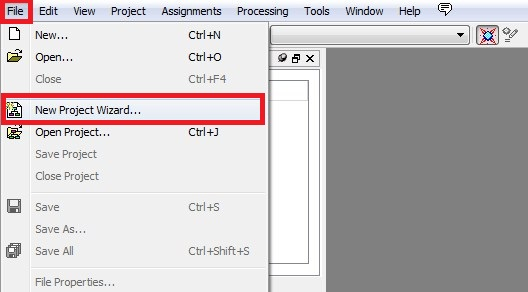
\includegraphics[scale=0.7]{1}
	\caption{UART settings}
	\label{fig:uart_settings}
\end{figure}
 
\begin{figure}[!h]
	\centering
	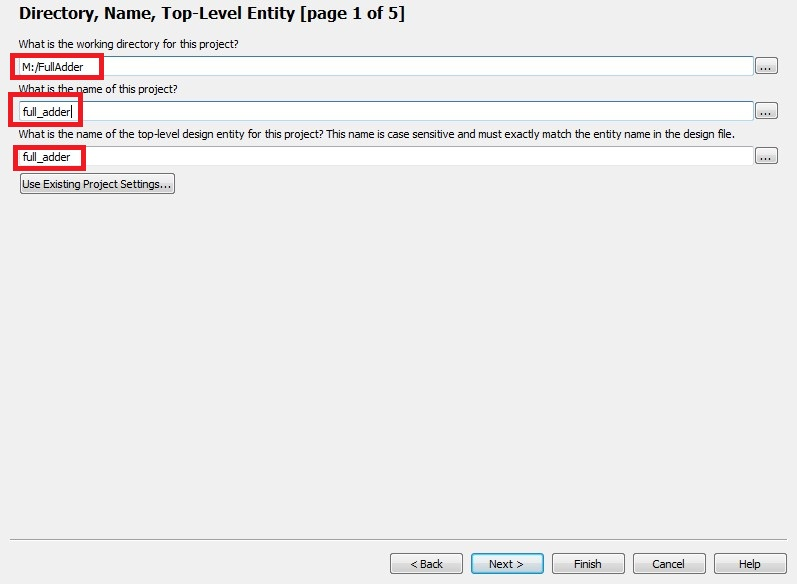
\includegraphics[scale=0.65]{2}
	\caption{Qsys connections}
	\label{fig:uart_qsys_conn}
\end{figure}

Now, add the file `Uart\_Qsys.qip' to the VHDL project. Next, create a new `Block diagram (.bdf) file and import the Qsys design to it and assign correct pin numbers to it, as shown in Fig. \ref{fig:uart_top}. Save it as `Uart\_top.bdf' and set it as `top  level entity'. Lastly, import the pin assignment file and compile the design. Finally, load the design on FPGA board. 

\begin{figure}[!h]
	\centering
	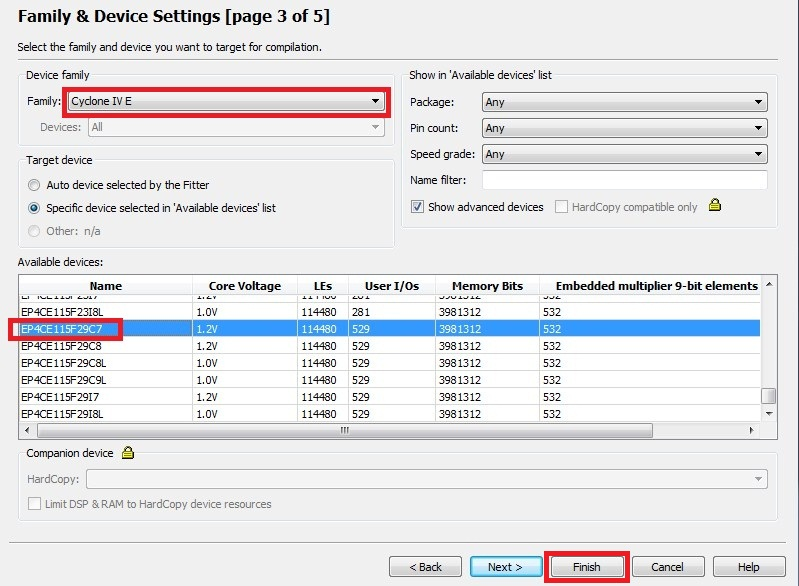
\includegraphics[scale=0.65]{3}
	\caption{Top level entity `Uart\_top.bdf'}
	\label{fig:uart_top}
\end{figure}

\section{NIOS design}
In Chapter \ref{ch:NiosOverview}, we created the `BSP' and `application' file separately for NIOS design. In this chapter, we will use the template provided with NIOS to create the design. For this, open the NIOS software and go to `Files$\rightarrow$New$\rightarrow$NIOS II Application and BSP from Template'. Next, Select the `UART\_Qsys.sopcinfo' file and `Hello World' template and provide the desired name to project e.g. UART\_comm\_app, as shown in Fig , and click `next'. In this window, enter the desired name for BSP file in the `Project name' column e.g. `UART\_comm\_bsp'; and click on Finish.  

\begin{figure}[!h]
	\centering
	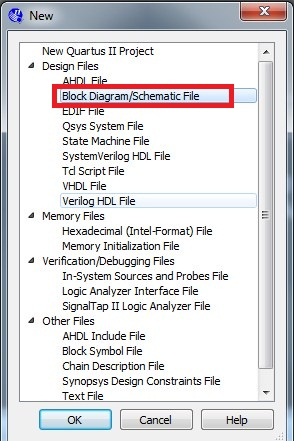
\includegraphics[scale=0.65]{4}
	\caption{Create NIOS project from template}
	\label{fig:nios_name_uart}
\end{figure}

\section{Communication through UART}
To received the data on computer, we need some software like Putty or Tera Term. In this tutorial, we are using `Tera Term software, which can be downloaded freely. Also, we need to change the UART communication settings; so that, we can get messages through UART interface (instead of JTAG-UART)  as shown next. 

Right click on `UART\_comm\_bsp' and go to `NIOS II$\rightarrow$BSP editor'; and select UART\_115200 for various communication as shown in Fig \ref{fig:nios_uart_settings}; and finally click on generate and then click on exit. Now, all the 	`printf' statements will be send to computer via UART port (instead of Jtag-uart). We can change it to JTAG-UART again, by changing UART\_115200 to JTAG-UART again. Note that, when we modify the BSP using BSP-editor, then we need to generate the system again.

\begin{figure}[!h]
	\centering
	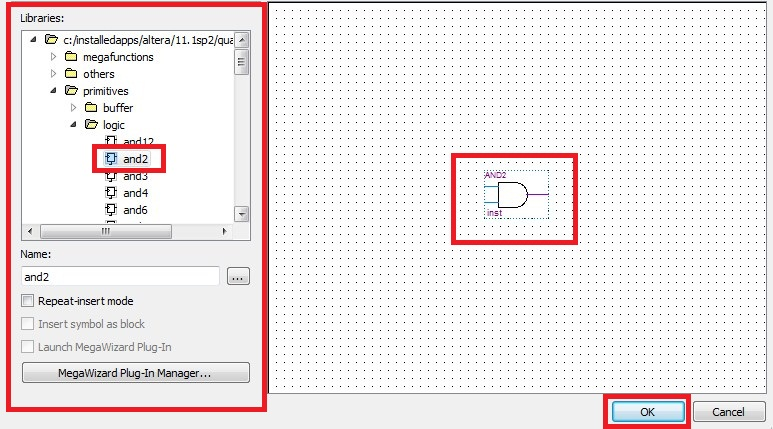
\includegraphics[scale=0.65]{5}
	\caption{UART communication settings in NIOS}
	\label{fig:nios_uart_settings}
\end{figure}

Now, open the Tera Term and select the `Serial' as shown in Fig. \ref{fig:teraTerm}. Then go to `Setup$\rightarrow$Serial Port...' and select the correct baud rate i.e. 115200 and click OK, as shown in Fig. \ref{fig:baudRateteraTerm}. 

\begin{figure}[!h]
	\centering
	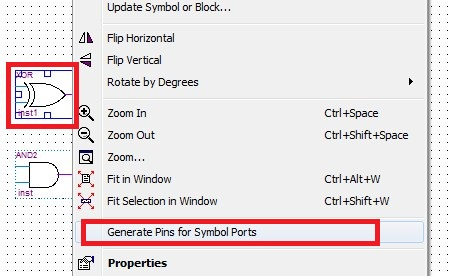
\includegraphics[scale=0.65]{6}
	\caption{Serial communication in Tera Term}
	\label{fig:teraTerm}
\end{figure}

\begin{figure}[!h]
	\centering
	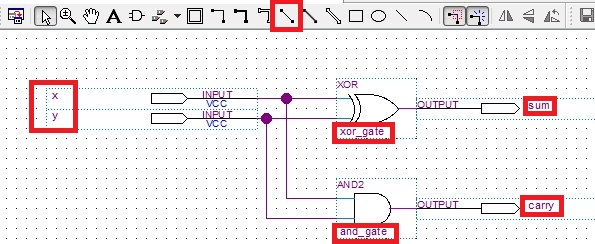
\includegraphics[scale=0.65]{7}
	\caption{Select correct baud rate}
	\label{fig:baudRateteraTerm}
\end{figure}

Finally, right click on `UART\_comm\_app' in NIOS and go to `Run As$\rightarrow$3 NIOS 2 Hardware'. Now, we can see the output on the Tera Term terminal, as shown in Fig. \ref{fig:helloTera}. 

\begin{figure}[!h]
	\centering
	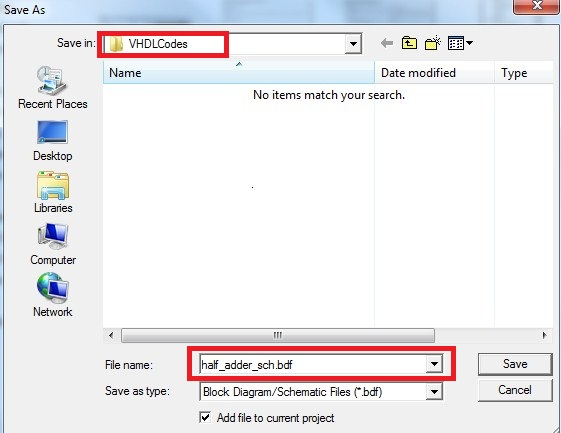
\includegraphics[scale=0.65]{8}
	\caption{`Hello from NIOS II!' on Tera Term}
	\label{fig:helloTera}
\end{figure}

\section{SDRAM Interface}
Our next aim is to generate the Sine waves using NIOS and then plot the waveforms using python. If we write the C-code in current design, then our system will report the memory issue as onchip memory is too small; therefore we need to use external memory. In this section, first, we will update the Qsys design with SDRAM interface, then we will update the Quartus design and finally add the C-code to generate the Sine waves. 

\subsection{Modify QSys}
First, Open the UART\_Qsys.qsys file in QSys software. Now, add SDRAM controller with default settings,  as shown in Fig. \ref{fig:sdram_con}. Next, connect all the ports of SDRMA as shown in Fig. \ref{fig:sdram_connections}. Then, double click the `nios2\_qsys\_0' and select `SDRAM' as reset and exception vector memory, as shown in Fig. \ref{fig:sdram_vector_memory}. 

\begin{figure}[!h]
	\centering
	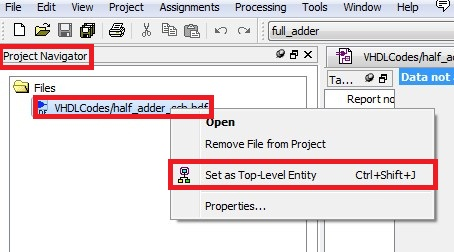
\includegraphics[scale=0.6]{9}
	\caption{SDRAM controller}
	\label{fig:sdram_con}
\end{figure}


\begin{figure}[!h]
	\centering
	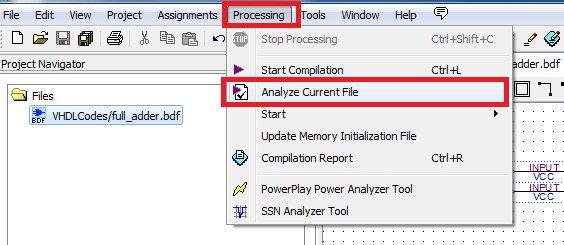
\includegraphics[scale=0.6]{10}
	\caption{SDRAM connections}
	\label{fig:sdram_connections}
\end{figure}


\begin{figure}[!h]
	\centering
	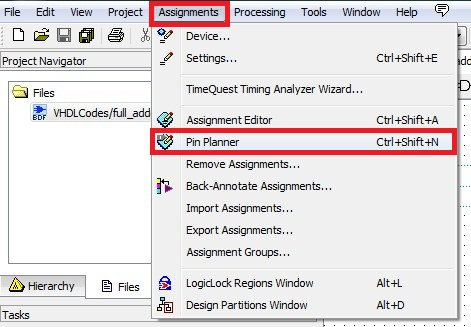
\includegraphics[scale=0.6]{11}
	\caption{Select SDRAM as vector memories}
	\label{fig:sdram_vector_memory}
\end{figure}


Next, we will add `Switches' to control the amplitude of the sine waves. For this add the PIO device of `8 bit with type input', and rename it as `switch', as shown in Fig. \ref{fig:switchForAmplitude} . Finally, go to System$\rightarrow$Assign base addresses, and generate the system. 

\begin{figure}[!h]
	\centering
	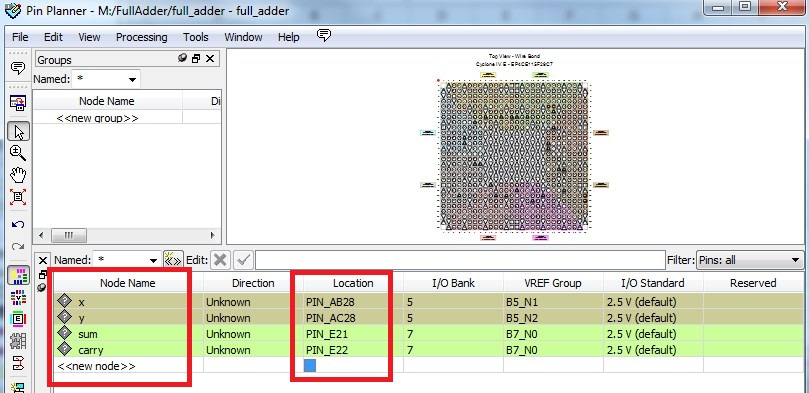
\includegraphics[scale=0.65]{12}
	\caption{Add switches for controlling the amplitude of sine waves}
	\label{fig:switchForAmplitude}
\end{figure}


\subsection{Modify Top level Quartus design}
Now, open the `Uart\_top.bdf' file in Quartus. Right click on the `Uart\_Qsys' block and select `Update symbol or block'; then select the option `Selected symbol(s) or block(s)' and press OK. It will display all the ports for `SDRAM' and switches. Next, we need to assign the correct `pin names' to these ports, as shown in Fig. \ref{fig:SDRAM_Pinassg}.  

\begin{figure}[!h]
	\centering
	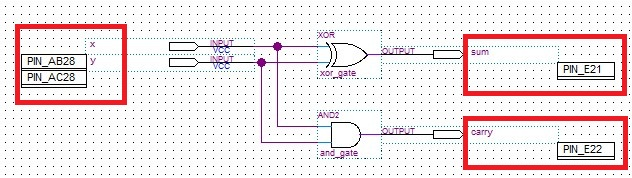
\includegraphics[scale=0.65]{13}
	\caption{Assigning Pins to SDRAM and Switches}
	\label{fig:SDRAM_Pinassg}
\end{figure}

Note that, there should be `-3 ns clock delay' for SDRAM as compare to FPGA clock, therefore we need to add the clock with `-3 ns delay'. For this, double click on the Uart\_top.bdf (anywhere in the file), and select `MegaWizard Plug-In Manager'. Then select `Create a new custom megafunction variation' in the popped-up window and click next. Now, select \textbf{ALTPLL} from \textbf{IO} in \textbf{Installed Plug-Ins} option, as shown in Fig. \ref{fig:dram_clock_altpll}, and click next. Then, follow the figures from Fig. \ref{fig:altpllCreation1} to Fig. \ref{fig:altpllCreation6} to add the ALTPLL to current design i.e. `Uart\_top.bdf'. Finally, connect the ports of this design as shown in Fig. \ref{fig:altpllCreation7}. Note that, in these connections, output of ATLPLL design is connected to `DRAM\_CLK', which is clock-port for DRAM. Lastly, compile and load the design on FPGA board. 

\begin{figure}[!h]
	\centering
	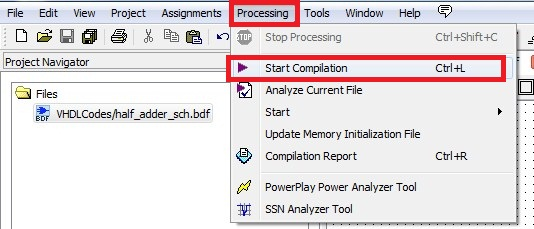
\includegraphics[scale=0.4]{14}
	\caption{ALTPLL generation}
	\label{fig:dram_clock_altpll}
\end{figure}

\begin{figure}[!h]
	\centering
	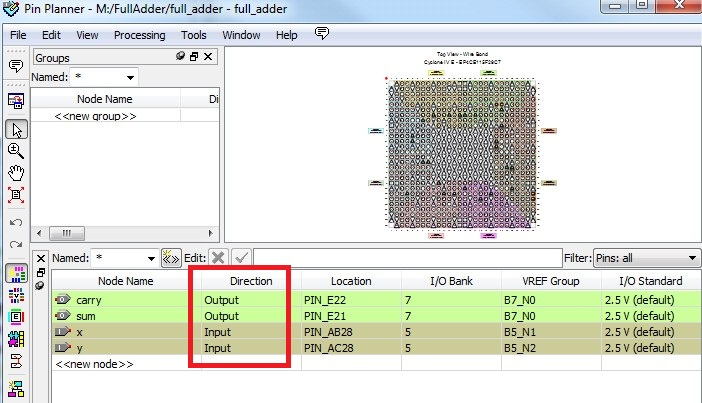
\includegraphics[scale=0.4]{15}
	\caption{ALTPLL creation, step 1}
	\label{fig:altpllCreation1}
\end{figure}

\begin{figure}[!h]
	\centering
	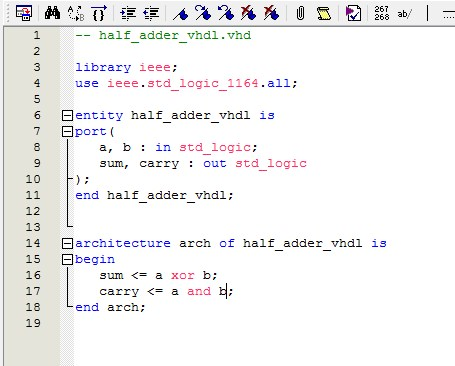
\includegraphics[scale=0.5]{16}
	\caption{ALTPLL creation, step 2}
	\label{fig:altpllCreation2}
\end{figure}

\begin{figure}[!h]
	\centering
	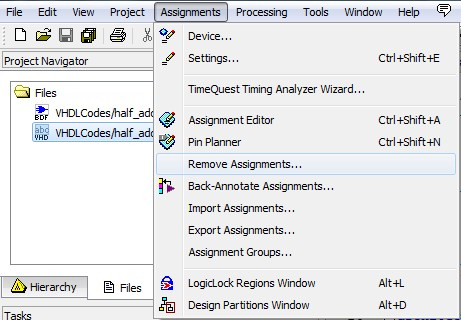
\includegraphics[scale=0.4]{17}
	\caption{ALTPLL creation, step 3}
	\label{fig:altpllCreation3}
\end{figure}

\begin{figure}[!h]
	\centering
	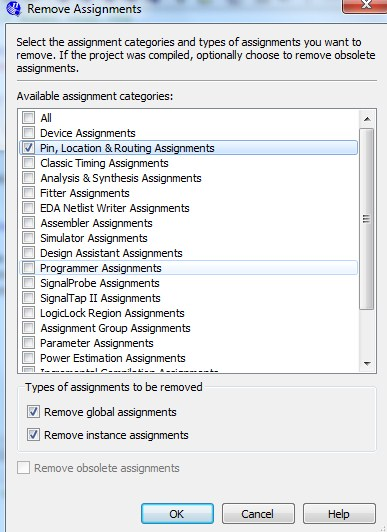
\includegraphics[scale=0.4]{18}
	\caption{ALTPLL creation, step 4}
	\label{fig:altpllCreation4}
\end{figure}

\begin{figure}[!h]
	\centering
	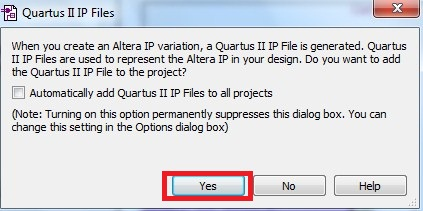
\includegraphics[scale=0.5]{19}
	\caption{ALTPLL creation, step 5}
	\label{fig:altpllCreation5}
\end{figure}

\begin{figure}[!h]
	\centering
	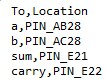
\includegraphics[scale=0.5]{20}
	\caption{ALTPLL creation, step 6}
	\label{fig:altpllCreation6}
\end{figure}

\begin{figure}[!h]
	\centering
	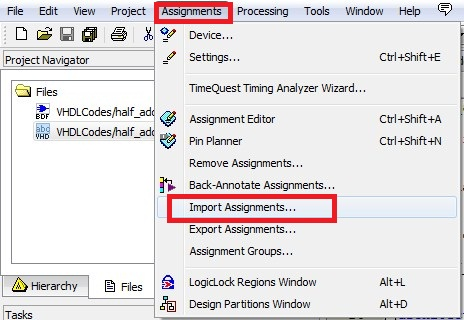
\includegraphics[scale=0.6]{21}
	\caption{Connect ALTPLL design with existing design}
	\label{fig:altpllCreation7}
\end{figure}

\subsection{Updating NIOS design}
Since, we have udpated the QSys design, therefore the corresponding .sopcinfo file is also updated. Further, BSP files depends on the .sopcinfo file, therefore we need to update the BSP as well. For this, right click on `Uart\_comm\_bsp' and go to `NIOS II$\rightarrow$BSP Editor; and update the BSP as shown in Fig. \ref{fig:updateBSPDRAM} and click on `generate' and then click `exit'. Note that, `enable' options are unchecked now, because we are using External memory, which is quite bigger than onchip-memory, so we do not need `small' size options. 

\begin{figure}[!h]
	\centering
	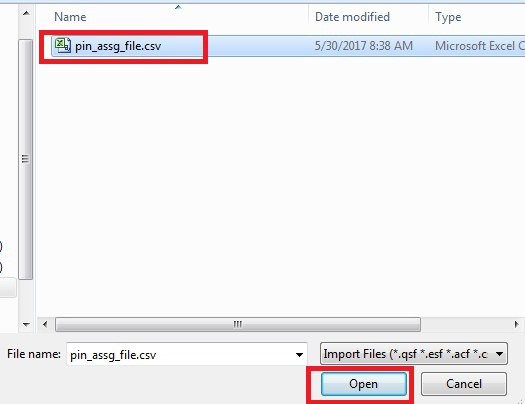
\includegraphics[scale=0.65]{22}
	\caption{Update BSP for new Qsys design}
	\label{fig:updateBSPDRAM}
\end{figure}

Now, update the `hello\_world.c' file as shown in Listing \ref{c:uart_sine_wave}. 

\lstinputlisting[
caption    = {Sin and Cos wave generation},
language = C,
label      = {c:uart_sine_wave}
]{CppCodes/hello_world.c}

In Tera Term, we can save the received values in text file as well. Next, go Files$\rightarrow$Log and select the filename at desired location to save the data e.g. `sineData.txt'. 

Finally, right click on `UART\_comm\_app' in NIOS and go to `Run As$\rightarrow$3 NIOS 2 Hardware'. Now, we can see the decimal values on the screen. If all the switches are at `0' position, then values will be `0.000' as amplitude is zero. Further, we can use any combination of 8 Switches to increase the amplitude of the sine and cosine waves. Also, result will be stored in the  `sineData.txt' file. Content of this file is shown in Fig. \ref{fig:contentLogFile}


\begin{figure}[!h]
	\centering
	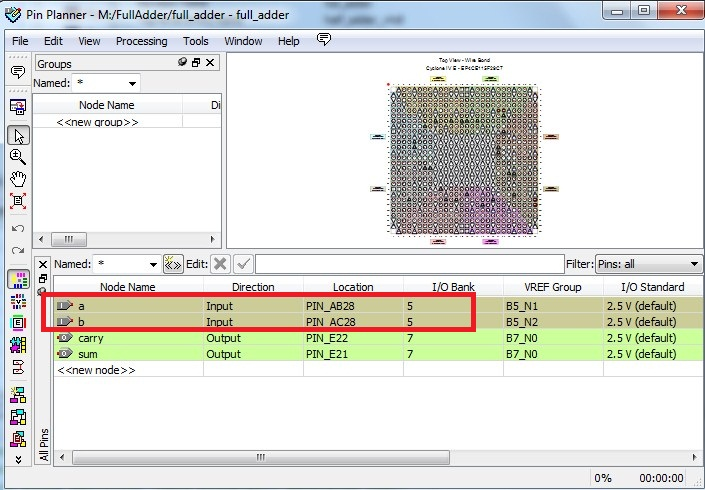
\includegraphics[scale=0.8]{23}
	\caption{Content of `sineData.txt' file}
	\label{fig:contentLogFile}
\end{figure}

\section{Live plotting the data}
In the previous section, we store the sine and cosine wave data on the `sineData.txt' using UART communication. Now, our last task is to plot this data continuously, so that it look line animation. For this save the Listing \ref{pythhon:plotLogData}, in the location where `sineData.txt' is saved. Now, open the command prompt and go to the location of python file. Finally, type \textbf{`python main.py'} and press enter. This will start plotting the waveform continuously based on the data received and stored on the `sineData.txt' file. The corresponding plots are shown in Fig. \ref{fig:plotLogFile}.

\lstinputlisting[
caption    = {Code for live plotting of logged data},
language = Python,
label      = {pythhon:plotLogData}
]{PythonCodes/main.py}

\begin{figure}[!h]
	\centering
	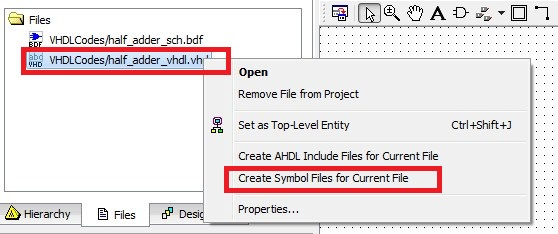
\includegraphics[scale=0.5]{24}
	\caption{Plot of `sineData.txt' file}
	\label{fig:plotLogFile}
\end{figure}


\section{Conclusion}
In this chapter, first we display the `Hello' message using UART and Tera Term. Then, SDRAM is included in the design and correspondingly all the other designs are updated i.e. Quartus and NIOS. Then, the data is stored in the text file and finally it is plotted with the help of Python programming language. 

\section{Introduction}
In this tutorial, full adder is designed with the help of half adders. Here we will learn following methods to create/implement the digital designs using Altera-Quartus software, 

\begin{enumerate}
	\item Digital design using `block schematics',
	\item Digital design using `VHDL codes',
	\item Manual pin assignment for implementation,
	\item Pin assignments using `.csv' file,
	\item Loading the design on FPGA. 
	\item Converting the `VHDL design' to `Symbols'
	\item Converting the `Block schematic' to `VHDL code' and `Symbols'. 
\end{enumerate}

If you do not have the FPGA-board, then skip the last part i.e. `loading the design on FPGA'. Simulation of the designs using `Modelsim' is discussed in Chapter \ref{ch:OverView}. 

\href{https://www.altera.com/downloads/software/quartus-ii-we/111sp2.html}{`Quartus II 11.1sp2 Web Edition'} and \href{https://www.altera.com/downloads/software/modelsim-starter/111.html}{`ModelSim-Altera Starter'} softwares are used for this tutorial, which are freely available and can be downloaded from the \href{https://www.altera.com/downloads/download-center.html}{Altera website}. All the codes can be \href{http://pythondsp.readthedocs.io/en/latest/pythondsp/toc.html}{downloaded from the website}. First line of each listing in the tutorial, is the name of the python file in the downloaded zip-folder. Also, see Appendix \ref{QuartusModelsim} to compile and synthesize the codes of the tutorial.

Note that, Altera-Modelsim-Starter version does not allow simulation of mixed design i.e. VHDL design mixed with Verilog can not be simulated. You need to buy the full edition of Altera-modelsim for this. Further, \href{https://www.aldec.com/en/products/fpga_simulation/active_hdl_student}{`Active-HDL student'} version can be downloaded for free and can be used for mixed-modeling simulation. Lastly, in Active-HDL, all the waveforms can be imported as `.vcd' format (if required); which can be used by Modelsim software as well. To use the .vcd file in Modelsim, first convert it into `.wlf' file. For this, first go to Modelsim's transcript window and then go to the desired directory (which contains the .vcd file) e.g. cd D:/VcdFiles; and then type conversion command i.e. `vcd2wlf VCD\_file\_name.vcd WLF\_file\_name.wlf. This will convert the .vcd file to .wlf file, which can be used in Modelsim to display waveforms.

\section{Creating the project} \label{sec:new_project}
\begin{enumerate}
	\item To create a new project, first open the Quartus and go to File$\rightarrow$New Project Wizard, as shown in Fig. \ref{fig:createNewProject}. 
	
	\begin{figure}[!h]
		\centering
		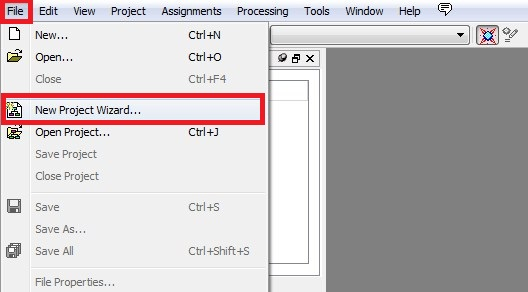
\includegraphics[scale=0.65]{1}
		\caption{Create new project}
		\label{fig:createNewProject}
	\end{figure}
	
	\item `Introduction' window will appear after this, click `next' and fill the project details as shown in Fig. \ref{fig:nameProject}. 
	
	\begin{figure}[!h]
		\centering
		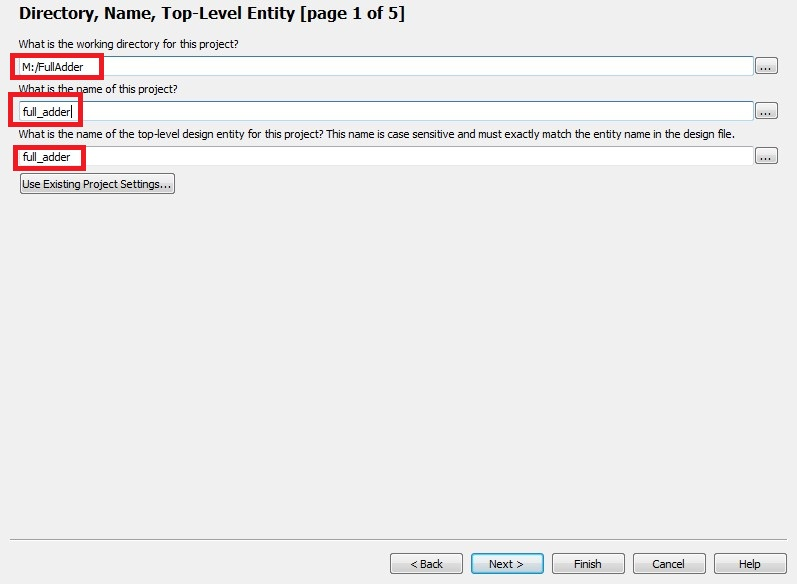
\includegraphics[scale=0.65]{2}
		\caption{Name and location of project}
		\label{fig:nameProject}
	\end{figure}
	
	\item After this, `Add files' window will appear, click on `next' here as we do not have any file to add to this project. 
	
	\item Next, `Family and Device settings' page will appear, select the proper device setting based on your FPGA board and click `Finish' as shown in Fig. \ref{fig:deviceSettings}. If you don't have FPGA board, then simply click `Finish'. 
	\begin{figure}[h]
		\centering
		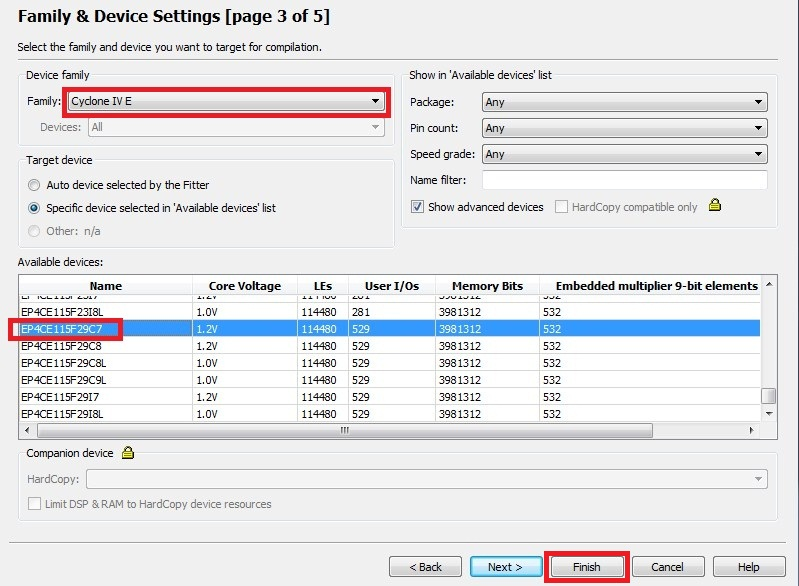
\includegraphics[scale=0.65]{3}
		\caption{Devices settings}
		\label{fig:deviceSettings}
	\end{figure}
	
	
	\item After clicking on finish, the project will be created as shown in Fig. \ref{fig:device_settings}. \textbf{Note that, the tutorials are tested on DE2-115, DE2 (cyclone-II family) or DE0-Nano boards, therefore project settings may be different for different chapters. You need to select the correct device while running the code on your system.} This can be done by double-clicking on the device name, as shown in Fig. \ref{fig:device_settings}.
	
	\begin{figure}[h]
		\centering
		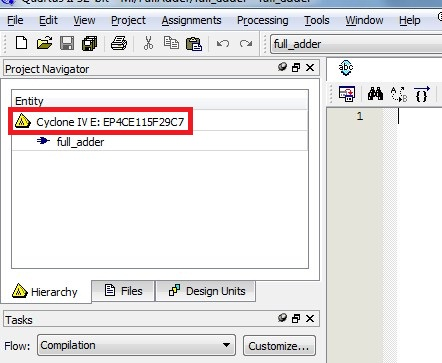
\includegraphics[scale=0.65]{device_settings}
		\caption{Updated Devices settings}
		\label{fig:device_settings}
	\end{figure}
\end{enumerate}

\section{ Digital design using `block schematics'}
Digitals design can be create using two methods i.e. using `block-schematics' and with programming language e.g. VHDL or verilog etc. Both have their own advantages in the design-process, as we will observe in the later chapters of the tutorials. 

In this section, we will create a half\_adder using block-schematics method, as shown below,

\begin{enumerate}
	
	\item For this, click on File$\rightarrow$New$\rightarrow$Block diagram/ Schematics files, as shown in Fig. \ref{fig:block_schematics}; and a blank file will be created.
	
	\begin{figure}
		\centering
		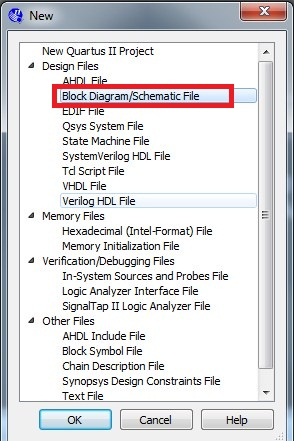
\includegraphics[scale=0.65]{4}
		\caption{Create new block schematics}
		\label{fig:block_schematics}
	\end{figure}
	
	\item Double click (anywhere) in the blank file, and a window will pop-up; select the `and' gate from this window as shown in Fig. \ref{fig:select_gate}. Similarly, select the `xor' gate. 
	
	\begin{figure}
		\centering
		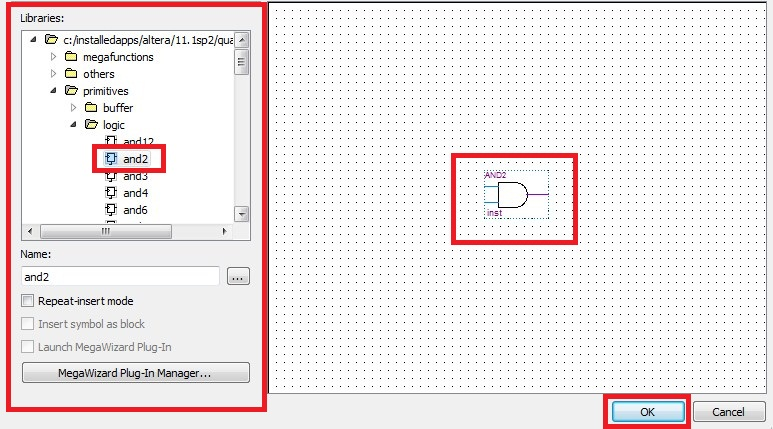
\includegraphics[scale=0.65]{5}
		\caption{Select `and' gate}
		\label{fig:select_gate}
	\end{figure}
	
	\item Next, right click on the `xor' gate and then click on `Generate Pins for Symbol Ports', as shown in Fig. \ref{fig:add_pins}. 
	
	\begin{figure}
		\centering
		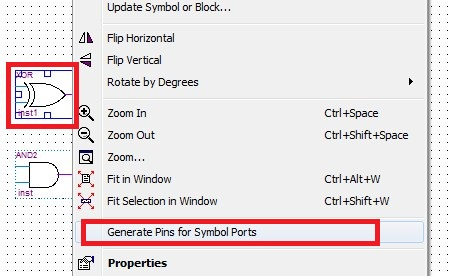
\includegraphics[scale=0.65]{6}
		\caption{Add ports}
		\label{fig:add_pins}
	\end{figure}
	
	\item Now, connect the input ports of `xor' gate with `and' gate (using mouse); then Next, right click on the `and' gate and then click on `Generate Pins for Symbol Ports'. Finally rename the input and output ports (i.e. x, y, sum and carry) as shown in Fig. \ref{fig:make_connections}. 
	
	\begin{figure}
		\centering
		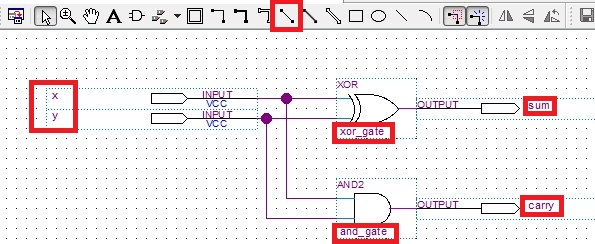
\includegraphics[scale=0.65]{7}
		\caption{Add ports}
		\label{fig:make_connections}
	\end{figure}
	
	\item Finally, save the design with name `half\_adder\_sch.bdf'. It's better to save the design in the separate folder, so that we can distinguish the user-defined and system-generated files, as shown in Fig. \ref{fig:save_project} where VHDL codes are saved inside the `VHDLCodes' folders, which is inside the main project directory. 
	
	\begin{figure}
		\centering
		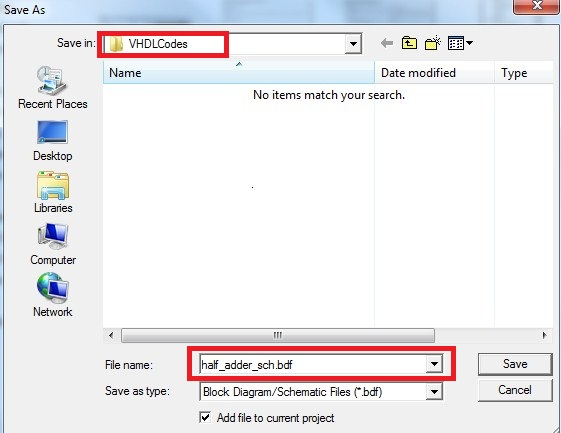
\includegraphics[scale=0.65]{8}
		\caption{Save project in separate directory i.e. VHDLCodes here}
		\label{fig:save_project}
	\end{figure}
	
	\item Since the project name is `full\_adder', where as the half adder's design name is `half\_adder\_sch.bdf' (i.e. not same as the project name), therefore we need to set this design as top level entity for compiling the project. For this, go to project navigator and right click on the `half\_adder\_sch.bdf' and set it as top level entity, as shown in Fig. \ref{fig:top_level_project}.  
	
	\begin{figure}
		\centering
		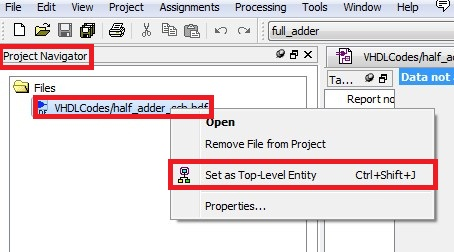
\includegraphics[scale=0.65]{9}
		\caption{Select top level entity for the project}
		\label{fig:top_level_project}
	\end{figure}
	
	\item Now, we can analyze the file as shown in Fig. \ref{fig:analyze_design}. If all the connections are correct that analysis option will not show any error. 
	
	Note that, `start compilation' option (above the Analyse option in the figure) is used when we want to generate the .sof/.pof file, to load the design on the FPGA, whereas analyze option only checks for the syntax errors. We will use `compilation' option in next section. 
	
	\begin{figure}
		\centering
		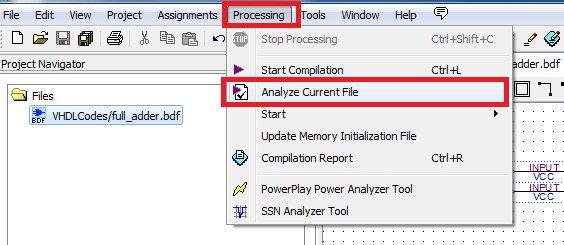
\includegraphics[scale=0.65]{10}
		\caption{Analyze the design}
		\label{fig:analyze_design}
	\end{figure}
	
\end{enumerate}

\section{Manual pin assignment and compilation} \label{sec:compile}\index{pin assignment!manual}
\textbf{Please enter correct pin location according to your FPGA board, as shown in this section. If you do not have the board, then skip this section and go to Section \ref{sec:digital_des_with_vhdl}.}
\\
\\	
Once design is analyzed, then next step is to assign the correct pin location to input and output ports. This can be done manually or using .csv file. In this section, we will assign pin manually. Follow the below steps for pin assignments, 

\begin{enumerate}
	\item First open the `Pin-planner' by clicking Assignments$\rightarrow$Pin Planner as shown in Fig. \ref{fig:pin_planner}.
	
	\begin{figure}
		\centering
		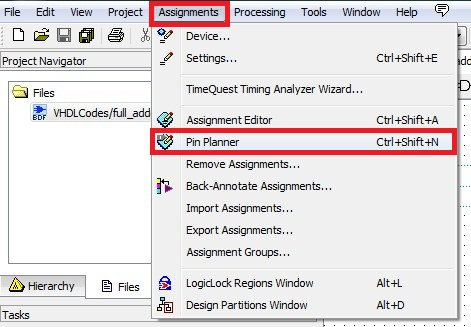
\includegraphics[scale=0.65]{11}
		\caption{Pin planner}
		\label{fig:pin_planner}
	\end{figure}
	
	\item Next, type the names of the input and output ports along with the pin-locations on the board, as shown in Fig. \ref{fig:pin_assgn}. Details of the Pin-locations are provided with the manual of the FPGA-boards e.g. in DE2-115 board, pin `PIN\_AB28' is connected with switch SW0. By assign this pin to `x', we are connecting the port `x' with switch SW0.
	
	\begin{figure}
		\centering
		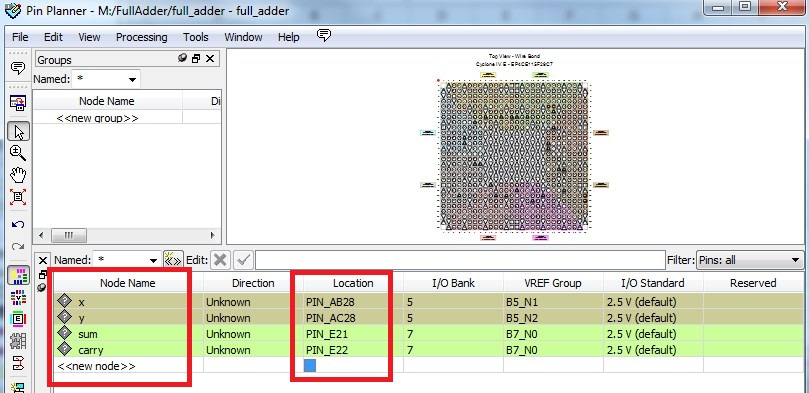
\includegraphics[scale=0.65]{12}
		\caption{Pin assignment}
		\label{fig:pin_assgn}
	\end{figure}
	
	\item After assigning the pin, analyse the design again (see Fig. \ref{fig:analyze_design}). After this, we can see the pin numbers in the `.bdf' file, as shown in Fig. \ref{fig:display_pin_assgn}.
	
	\begin{figure}
		\centering
		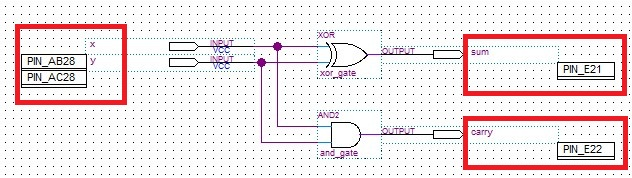
\includegraphics[scale=0.65]{13}
		\caption{Assigned pins to ports}
		\label{fig:display_pin_assgn}
	\end{figure}
	
	\item Finally, compile the design using `ctrl+L' button (or by clicking processing$\rightarrow$Start compilation, as shown in Fig. \ref{fig:start_compilation}). 
	
	\begin{figure}
		\centering
		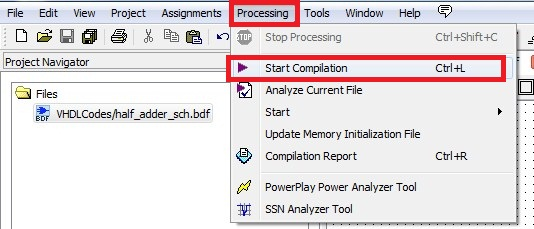
\includegraphics[scale=0.65]{14}
		\caption{Start compilation}
		\label{fig:start_compilation}
	\end{figure}	
	
	\item After successful compilation, if we see the pin-assignment again, then we will find that direction of the pin are assigned now, as shown in Fig. \ref{fig:pin_assgn_direction} (which were set to `unknown' during analysis as in Fig. \ref{fig:pin_assgn})
	
	\begin{figure}[!h]
		\centering
		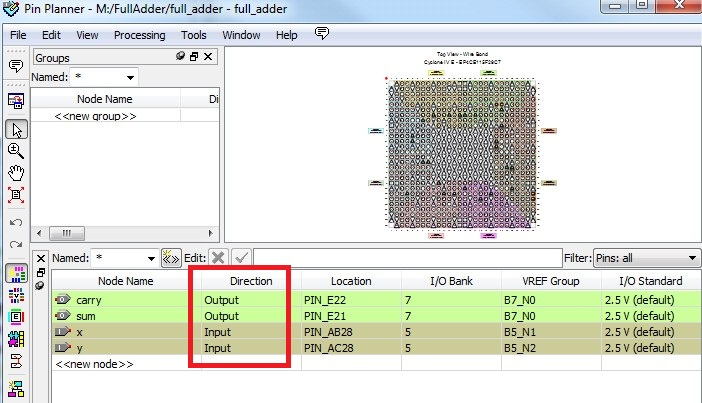
\includegraphics[scale=0.65]{15}
		\caption{Direction of the ports}
		\label{fig:pin_assgn_direction}
	\end{figure}
	
\end{enumerate}

\section{Load the design on FPGA} \label{sec:load_fpga_design}

Follow the below, steps to load the design on FPGA, 

\begin{enumerate}
	\item Connect the FPGA to computer and turn it on. 
	
	\item Full compilation process (Section \ref{sec:compile}), generates the .sof/.pof files, which can be loaded on the FPGA board. To load the design on FPGA board, go to \textbf{Tools$\rightarrow$Programmer}. And a programmer window will pop up. 
	
	\item In the programmer window (see Fig. \ref{fig:load_design}), look for two things i.e. position `1' should display `USB-BLASTER' and position `6' should display the `.sof' file. If any of this mission then follow below steps, 
	
	\begin{itemize}
		\item If USB-BLASTER is missing, then click on `Hardware setup (location 2 in Fig. \ref{fig:load_design})' and then double click on USB-BLASTER in the pop-up window (location 3). This will display the USB-BLASTER at location 4. Finally close the pop-up window. 
		
		\item If `.sof' file is not displayed at location 6, then click on `Add file...' (location 7) and select the `.sof' file from main project directory (or in output\_files folder in main project diretory).
	\end{itemize} 
	
	\item Finally click on the `start' button in Fig. \ref{fig:load_design} and check the operation of `half adder' using switches SW0 and SW1; output will be displayed on green LEDs i.e. LEDG0 and LEDG1. 
	
	\begin{figure}[!h]
		\centering
		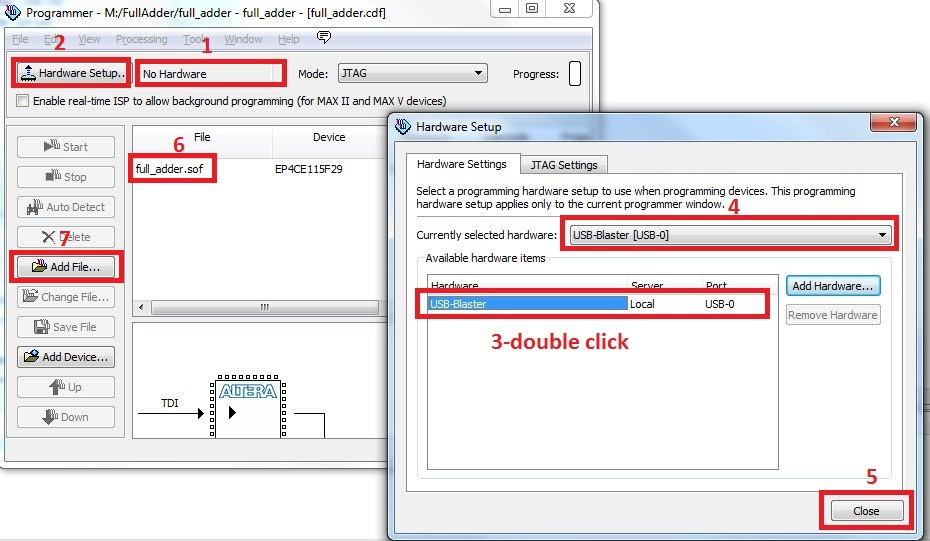
\includegraphics[width=\textwidth]{load_design}
		\caption{Load the design on FPGA}
		\label{fig:load_design}
	\end{figure}
\end{enumerate}

\section{Digital design using `VHDL codes'} \label{sec:digital_des_with_vhdl}

In this section, half adder is implemented using VHDL codes. For this, click on File$\rightarrow$New$\rightarrow$VHDL files, as shown in Fig. \ref{fig:block_schematics}; and a blank file will be created. Type the Listing \ref{vhdl:half_adder_vhdl} in this file and save it as `half\_adder\_vhdl.vhd'. 

\textbf{Now, set this design as `top level entity' (Fig. \ref{fig:top_level_project}).} We can analyze the design now, but we will do it after assigning the pins using .csv file in next section.

\lstinputlisting[
language = Vhdl,
caption    = {VHDL code for half adder},
label      = {vhdl:half_adder_vhdl}
]{half_adder_vhdl.vhd}

\section{Pin assignments using `.csv' file}\index{pin assignment!csv}
In this section, we will learn to assign the pins using .csv files. For this. Note that, we used input port as `a' and `b' in VHDL design (instead of `x' and `y' as in Fig. \ref{fig:make_connections}), so that we can observe the change in the pin assignments. 

To assign the pins using csv file, follow the below steps, 

\begin{enumerate}
	\item First type the content in Fig. \ref{fig:pin_ass_csv} in a text-file and save it as `pin\_assg\_file.csv'. 
	
	\begin{figure}[!h]
		\centering
		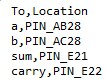
\includegraphics[scale=1]{20}
		\caption{Content of pin\_assg\_file.csv}
		\label{fig:pin_ass_csv}
	\end{figure}
	
	\item Next, click on the Assignments$\rightarrow$Import Assignments as shown in Fig. \ref{fig:import_assg}. And locate the file pin\_assg\_file.csv by clicking on the $\cdots$ button, in the popped-up window, as shown in Fig. \ref{fig:locate_assg}. 
	
	\begin{figure}
		\centering
		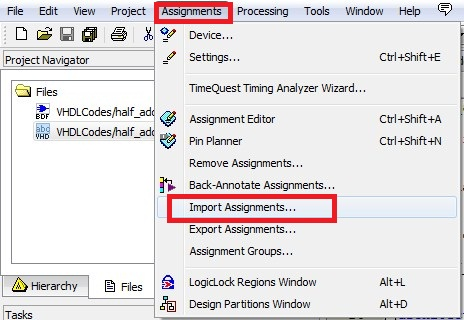
\includegraphics[scale=0.65]{21}
		\caption{Import assignments}
		\label{fig:import_assg}
	\end{figure}
	
	\begin{figure}[!h]
		\centering
		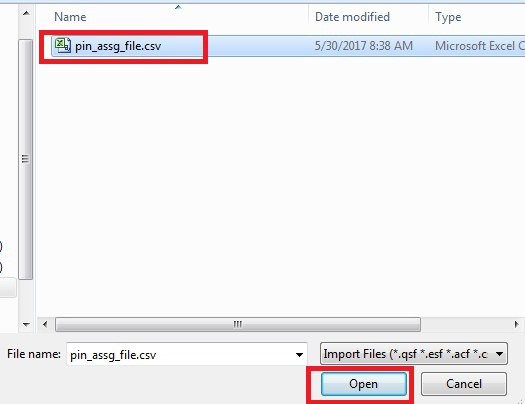
\includegraphics[scale=0.65]{22}
		\caption{Locate the csv file}
		\label{fig:locate_assg}
	\end{figure}
	
	\item Now, analyze the design (Fig. \ref{fig:analyze_design}) and then open the pin planner (Fig. \ref{fig:pin_planner}). We can see the new pin assignments as shown in Fig. \ref{fig:pin_assg_from_csv} (If proper assignments do not happen then check, whether the VHDL design is set as top level or not and import assignments again and analyze the design). 
	
	\begin{figure}
		\centering
		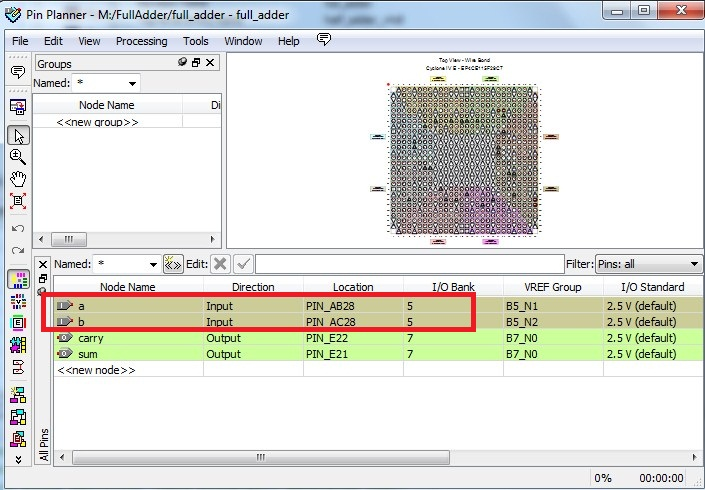
\includegraphics[scale=0.65]{23}
		\caption{Pin assignments from csv file}
		\label{fig:pin_assg_from_csv}
	\end{figure}
	
	\item Finally, compile and load and check the design as discussed in Section \ref{sec:load_fpga_design}. 
\end{enumerate}


\section{Converting the VHDL design to symbol} \label{sec:vhdl_to_symbol}
VHDL code can be converted into block schematic format,  which is quite useful for connecting various modules together. In this section, half adder's vhdl file is converted into schematic and then two half adder is connected to make a full adder. Note that, this connection can be made using VHDL code as well, which is discussed in Chapter \ref{ch:OverView}. 

Follow the below steps to create a full adder using this method,


\begin{enumerate}
	\item Right click on the `half\_adder\_vhdl.vhd' and click on `Create symbol file for current file' as shown in Fig. \ref{fig:vhdl_to_symbol}. It will create a symbol for half adder design. 
	
	\begin{figure}
		\centering
		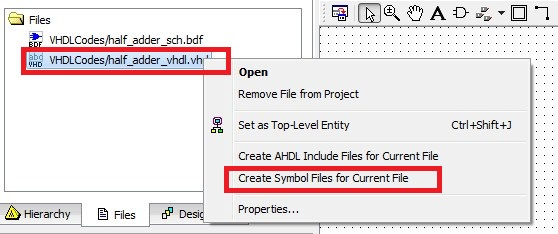
\includegraphics[scale=0.65]{24}
		\caption{Convert VHDL code to symbol}
		\label{fig:vhdl_to_symbol}
	\end{figure}
	%	
	\item Now, create a new `block schematic file' (Fig. \ref{fig:block_schematics}). 
	\item Next, double click on this file and add the half adder symbol as shown in Fig. \ref{fig:ha_symbol}.
	
	\begin{figure}
		\centering
		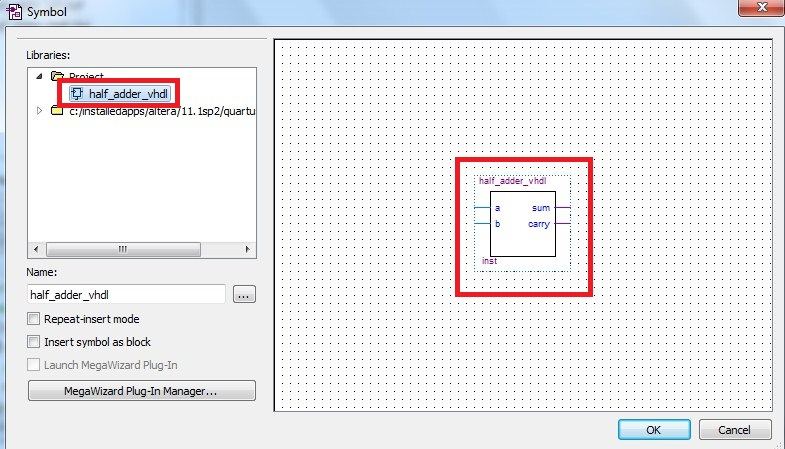
\includegraphics[scale=0.65]{25}
		\caption{Add half adder symbol}
		\label{fig:ha_symbol}
	\end{figure}
	%	
	\item Again add one more `half adder symbol' along with `or' gate and connect these components as shown in Fig. \ref{fig:fa_design}. 
	
	\begin{figure}
		\centering
		\includegraphics[scale=0.65]{26}
		\caption{Full adder using half adders}
		\label{fig:fa_design}
	\end{figure}
	
	\item Since, one more port (i.e. c) is added to the design, therefore modify the `pin\_assg\_file.csv' as shown in Fig. \ref{fig:update_pin_assg}. 
	
	\begin{figure}
		\centering
		\includegraphics[scale=1]{27}
		\caption{Full adder using half adders}
		\label{fig:update_pin_assg}
	\end{figure}
	%		
	\item Save the design as `full\_adder\_sch.bdf'. 
	\item Import the assignment again; and compile the design (see pin assignments as well for 5 ports i.e. a, b, c, sum and carry). Finally load the design on FGPA. 
\end{enumerate}

\section{Convert Block schematic to `VHDL code' and `Symbol'}

We can convert the `.bdf' file to VHDL code as well. In this section, full adder design is converted to VHDL code. For this open the file `full\_adder\_sch.bdf'. Then go to File$\rightarrow$Create/Update$\rightarrow$Create HDL Design File... as shown in Fig. \ref{fig:bdf_to_vhdl} and select the file type as `VHDL' and press OK; the file will be saved in the VHDLCodes folder (see Fig. \ref{fig:to_vhdl}). The content of the generated `VHDL' file are shown in Listing \ref{vhdl:full_adder_sch}. 

Now, we can convert this VHDL code into symbol as shown in Section \ref{sec:vhdl_to_symbol}. 

\begin{noNumBox}
	Note that, if we can to convert the `.bdf' file into symbol, then we need to convert it into VHDL code first, and then we can convert the VHDL code into symbol file. 
\end{noNumBox}

\begin{figure}[!h]
	\centering
	\includegraphics[width=\textwidth]{29}
	\caption{Convert schematic to VHDL}
	\label{fig:bdf_to_vhdl}
\end{figure}


\begin{figure}[!h]
	\centering
	\includegraphics[scale=0.65]{31}
	\caption{Select VHDL}
	\label{fig:to_vhdl}
\end{figure}

\lstinputlisting[
language = Vhdl,
caption    = {VHDL code for full adder},
label      = {vhdl:full_adder_sch}
]{full_adder_sch.vhd}

\section{Conclusion}
In this chapter, we learn to implement the design using schematic and coding methods. Also, we did the pin assignments manually as well as using csv file. Finally, we learn to convert the VHDL code into symbol file; and schematic design into VHDL code. 

\begin{noNumBox}
	Please see the Appendix \ref{NiosQuartusModelsim}  as well, where some more details about symbol connections are shown, along with the methods for using the codes provided in this tutorial. 
\end{noNumBox}

\chapter{Overview} \label{ch:OverView}
\chapterquote{That is real service where there is no thought of self at all.}{Meher Baba}

\graphicspath{{Chapters/Overview/Figures/}}
\lstinputpath{Codes-VHDL/Chapter-Overview/VHDLCodes/} %path is defined in mypreamble


\section{Introduction}
In this chapter, UART communication is discussed for NIOS design. Values of Sin(x) is generated using NIOS and the data is  received by computer using UART cable. Since, onchip memory is smaller for storing these values, therefore external memory i.e. SDRAM is used. Further, the received data is stored in a file using `Tera Term' software; finally live-plotting of data is performed using Python.  

In this chapter, we will learn following topics, 
\begin{enumerate}
	\item UART interface,
	\item Receiving the data on computer using UART communication,
	\item SDRAM interface,
	\item Saving data generated by NIOS desgin to a file using `Tera Term',
	\item Updating a existing QSys design and corresponding VHDL and NIOS design,
	\item Live-plotting of data using Python. 
\end{enumerate}

\section{UART interface}
First, create a empty project with name `UartComm' (see Section \ref{sec:new_project}). Next, open the QSys from Tools$\rightarrow$Qsys. Add `Nios Processor', `On-chip RAM (with 20k total-memory-size), `JTAG UART' and `UART (RS-232 Serial Port)' (\textbf{all with default settings}). Note that, Baud rate for UART is set to `115200' (see Fig. \ref{fig:uart_settings}), which will be used while getting the data on computer. Lastly, connect these items as shown in Fig. \ref{fig:uart_qsys_conn}; save it as `Uart\_Qsys.qsys' and finally generate the Qsys system and close the Qsys. Please see Section \ref{sec:CreateGenerateQsys}, if you have problem in generating the QSys system.

\begin{figure}[!h]
	\centering
	\includegraphics[scale=0.7]{1}
	\caption{UART settings}
	\label{fig:uart_settings}
\end{figure}
 
\begin{figure}[!h]
	\centering
	\includegraphics[scale=0.65]{2}
	\caption{Qsys connections}
	\label{fig:uart_qsys_conn}
\end{figure}

Now, add the file `Uart\_Qsys.qip' to the VHDL project. Next, create a new `Block diagram (.bdf) file and import the Qsys design to it and assign correct pin numbers to it, as shown in Fig. \ref{fig:uart_top}. Save it as `Uart\_top.bdf' and set it as `top  level entity'. Lastly, import the pin assignment file and compile the design. Finally, load the design on FPGA board. 

\begin{figure}[!h]
	\centering
	\includegraphics[scale=0.65]{3}
	\caption{Top level entity `Uart\_top.bdf'}
	\label{fig:uart_top}
\end{figure}

\section{NIOS design}
In Chapter \ref{ch:NiosOverview}, we created the `BSP' and `application' file separately for NIOS design. In this chapter, we will use the template provided with NIOS to create the design. For this, open the NIOS software and go to `Files$\rightarrow$New$\rightarrow$NIOS II Application and BSP from Template'. Next, Select the `UART\_Qsys.sopcinfo' file and `Hello World' template and provide the desired name to project e.g. UART\_comm\_app, as shown in Fig , and click `next'. In this window, enter the desired name for BSP file in the `Project name' column e.g. `UART\_comm\_bsp'; and click on Finish.  

\begin{figure}[!h]
	\centering
	\includegraphics[scale=0.65]{4}
	\caption{Create NIOS project from template}
	\label{fig:nios_name_uart}
\end{figure}

\section{Communication through UART}
To received the data on computer, we need some software like Putty or Tera Term. In this tutorial, we are using `Tera Term software, which can be downloaded freely. Also, we need to change the UART communication settings; so that, we can get messages through UART interface (instead of JTAG-UART)  as shown next. 

Right click on `UART\_comm\_bsp' and go to `NIOS II$\rightarrow$BSP editor'; and select UART\_115200 for various communication as shown in Fig \ref{fig:nios_uart_settings}; and finally click on generate and then click on exit. Now, all the 	`printf' statements will be send to computer via UART port (instead of Jtag-uart). We can change it to JTAG-UART again, by changing UART\_115200 to JTAG-UART again. Note that, when we modify the BSP using BSP-editor, then we need to generate the system again.

\begin{figure}[!h]
	\centering
	\includegraphics[scale=0.65]{5}
	\caption{UART communication settings in NIOS}
	\label{fig:nios_uart_settings}
\end{figure}

Now, open the Tera Term and select the `Serial' as shown in Fig. \ref{fig:teraTerm}. Then go to `Setup$\rightarrow$Serial Port...' and select the correct baud rate i.e. 115200 and click OK, as shown in Fig. \ref{fig:baudRateteraTerm}. 

\begin{figure}[!h]
	\centering
	\includegraphics[scale=0.65]{6}
	\caption{Serial communication in Tera Term}
	\label{fig:teraTerm}
\end{figure}

\begin{figure}[!h]
	\centering
	\includegraphics[scale=0.65]{7}
	\caption{Select correct baud rate}
	\label{fig:baudRateteraTerm}
\end{figure}

Finally, right click on `UART\_comm\_app' in NIOS and go to `Run As$\rightarrow$3 NIOS 2 Hardware'. Now, we can see the output on the Tera Term terminal, as shown in Fig. \ref{fig:helloTera}. 

\begin{figure}[!h]
	\centering
	\includegraphics[scale=0.65]{8}
	\caption{`Hello from NIOS II!' on Tera Term}
	\label{fig:helloTera}
\end{figure}

\section{SDRAM Interface}
Our next aim is to generate the Sine waves using NIOS and then plot the waveforms using python. If we write the C-code in current design, then our system will report the memory issue as onchip memory is too small; therefore we need to use external memory. In this section, first, we will update the Qsys design with SDRAM interface, then we will update the Quartus design and finally add the C-code to generate the Sine waves. 

\subsection{Modify QSys}
First, Open the UART\_Qsys.qsys file in QSys software. Now, add SDRAM controller with default settings,  as shown in Fig. \ref{fig:sdram_con}. Next, connect all the ports of SDRMA as shown in Fig. \ref{fig:sdram_connections}. Then, double click the `nios2\_qsys\_0' and select `SDRAM' as reset and exception vector memory, as shown in Fig. \ref{fig:sdram_vector_memory}. 

\begin{figure}[!h]
	\centering
	\includegraphics[scale=0.6]{9}
	\caption{SDRAM controller}
	\label{fig:sdram_con}
\end{figure}


\begin{figure}[!h]
	\centering
	\includegraphics[scale=0.6]{10}
	\caption{SDRAM connections}
	\label{fig:sdram_connections}
\end{figure}


\begin{figure}[!h]
	\centering
	\includegraphics[scale=0.6]{11}
	\caption{Select SDRAM as vector memories}
	\label{fig:sdram_vector_memory}
\end{figure}


Next, we will add `Switches' to control the amplitude of the sine waves. For this add the PIO device of `8 bit with type input', and rename it as `switch', as shown in Fig. \ref{fig:switchForAmplitude} . Finally, go to System$\rightarrow$Assign base addresses, and generate the system. 

\begin{figure}[!h]
	\centering
	\includegraphics[scale=0.65]{12}
	\caption{Add switches for controlling the amplitude of sine waves}
	\label{fig:switchForAmplitude}
\end{figure}


\subsection{Modify Top level Quartus design}
Now, open the `Uart\_top.bdf' file in Quartus. Right click on the `Uart\_Qsys' block and select `Update symbol or block'; then select the option `Selected symbol(s) or block(s)' and press OK. It will display all the ports for `SDRAM' and switches. Next, we need to assign the correct `pin names' to these ports, as shown in Fig. \ref{fig:SDRAM_Pinassg}.  

\begin{figure}[!h]
	\centering
	\includegraphics[scale=0.65]{13}
	\caption{Assigning Pins to SDRAM and Switches}
	\label{fig:SDRAM_Pinassg}
\end{figure}

Note that, there should be `-3 ns clock delay' for SDRAM as compare to FPGA clock, therefore we need to add the clock with `-3 ns delay'. For this, double click on the Uart\_top.bdf (anywhere in the file), and select `MegaWizard Plug-In Manager'. Then select `Create a new custom megafunction variation' in the popped-up window and click next. Now, select \textbf{ALTPLL} from \textbf{IO} in \textbf{Installed Plug-Ins} option, as shown in Fig. \ref{fig:dram_clock_altpll}, and click next. Then, follow the figures from Fig. \ref{fig:altpllCreation1} to Fig. \ref{fig:altpllCreation6} to add the ALTPLL to current design i.e. `Uart\_top.bdf'. Finally, connect the ports of this design as shown in Fig. \ref{fig:altpllCreation7}. Note that, in these connections, output of ATLPLL design is connected to `DRAM\_CLK', which is clock-port for DRAM. Lastly, compile and load the design on FPGA board. 

\begin{figure}[!h]
	\centering
	\includegraphics[scale=0.4]{14}
	\caption{ALTPLL generation}
	\label{fig:dram_clock_altpll}
\end{figure}

\begin{figure}[!h]
	\centering
	\includegraphics[scale=0.4]{15}
	\caption{ALTPLL creation, step 1}
	\label{fig:altpllCreation1}
\end{figure}

\begin{figure}[!h]
	\centering
	\includegraphics[scale=0.5]{16}
	\caption{ALTPLL creation, step 2}
	\label{fig:altpllCreation2}
\end{figure}

\begin{figure}[!h]
	\centering
	\includegraphics[scale=0.4]{17}
	\caption{ALTPLL creation, step 3}
	\label{fig:altpllCreation3}
\end{figure}

\begin{figure}[!h]
	\centering
	\includegraphics[scale=0.4]{18}
	\caption{ALTPLL creation, step 4}
	\label{fig:altpllCreation4}
\end{figure}

\begin{figure}[!h]
	\centering
	\includegraphics[scale=0.5]{19}
	\caption{ALTPLL creation, step 5}
	\label{fig:altpllCreation5}
\end{figure}

\begin{figure}[!h]
	\centering
	\includegraphics[scale=0.5]{20}
	\caption{ALTPLL creation, step 6}
	\label{fig:altpllCreation6}
\end{figure}

\begin{figure}[!h]
	\centering
	\includegraphics[scale=0.6]{21}
	\caption{Connect ALTPLL design with existing design}
	\label{fig:altpllCreation7}
\end{figure}

\subsection{Updating NIOS design}
Since, we have udpated the QSys design, therefore the corresponding .sopcinfo file is also updated. Further, BSP files depends on the .sopcinfo file, therefore we need to update the BSP as well. For this, right click on `Uart\_comm\_bsp' and go to `NIOS II$\rightarrow$BSP Editor; and update the BSP as shown in Fig. \ref{fig:updateBSPDRAM} and click on `generate' and then click `exit'. Note that, `enable' options are unchecked now, because we are using External memory, which is quite bigger than onchip-memory, so we do not need `small' size options. 

\begin{figure}[!h]
	\centering
	\includegraphics[scale=0.65]{22}
	\caption{Update BSP for new Qsys design}
	\label{fig:updateBSPDRAM}
\end{figure}

Now, update the `hello\_world.c' file as shown in Listing \ref{c:uart_sine_wave}. 

\lstinputlisting[
caption    = {Sin and Cos wave generation},
language = C,
label      = {c:uart_sine_wave}
]{CppCodes/hello_world.c}

In Tera Term, we can save the received values in text file as well. Next, go Files$\rightarrow$Log and select the filename at desired location to save the data e.g. `sineData.txt'. 

Finally, right click on `UART\_comm\_app' in NIOS and go to `Run As$\rightarrow$3 NIOS 2 Hardware'. Now, we can see the decimal values on the screen. If all the switches are at `0' position, then values will be `0.000' as amplitude is zero. Further, we can use any combination of 8 Switches to increase the amplitude of the sine and cosine waves. Also, result will be stored in the  `sineData.txt' file. Content of this file is shown in Fig. \ref{fig:contentLogFile}


\begin{figure}[!h]
	\centering
	\includegraphics[scale=0.8]{23}
	\caption{Content of `sineData.txt' file}
	\label{fig:contentLogFile}
\end{figure}

\section{Live plotting the data}
In the previous section, we store the sine and cosine wave data on the `sineData.txt' using UART communication. Now, our last task is to plot this data continuously, so that it look line animation. For this save the Listing \ref{pythhon:plotLogData}, in the location where `sineData.txt' is saved. Now, open the command prompt and go to the location of python file. Finally, type \textbf{`python main.py'} and press enter. This will start plotting the waveform continuously based on the data received and stored on the `sineData.txt' file. The corresponding plots are shown in Fig. \ref{fig:plotLogFile}.

\lstinputlisting[
caption    = {Code for live plotting of logged data},
language = Python,
label      = {pythhon:plotLogData}
]{PythonCodes/main.py}

\begin{figure}[!h]
	\centering
	\includegraphics[scale=0.5]{24}
	\caption{Plot of `sineData.txt' file}
	\label{fig:plotLogFile}
\end{figure}


\section{Conclusion}
In this chapter, first we display the `Hello' message using UART and Tera Term. Then, SDRAM is included in the design and correspondingly all the other designs are updated i.e. Quartus and NIOS. Then, the data is stored in the text file and finally it is plotted with the help of Python programming language. 
\section{Entity and Architecture}
In this section, we discuss `entity declaration' and `architecture body' along with three different ways of modeling i.e. `data flow', 'structural' and `behavioral' modeling. In practice, these three styles are mixed together to model a digital circuit.  

\subsection{Entity declaration}
In Fig. \ref{fig:andEx}, a simple `and' gate is shown; which is generated by Listing \ref{vhdl:andEx}. Listing \ref{vhdl:andEx} is included to understand the meaning of `entity declaration' and `architecture body'. Also in VHDL, `$--$' is used for comments; please read comments as well to understand the codes.

The entity declaration (lines 6-11) contains all the name of the input and outputs ports as shown in Listing \ref{vhdl:andEx}. Here, the design has two input ports i.e. $x$ and $y$ and one output port i.e. $z$, which are defined inside the `port' block in line 7. Name of the entity `andEx' is defined in line 6. Lastly, we need to import libraries to the listing which contains various functions e.g. library `IEEE' (line 3) contains the package `std\_logic\_1164' (line 4), in which `std\_logic' is defined. `std\_logic' is used in line 8 and 9, to define the 1-bit input and output data-types. Lastly, entity block is closed with `end' keyword in line 11. All these terms, i.e. IEEE library and packages along with data-types, are discussed in detail in Chapter \ref{ch:Datatypes}.  

\begin{figure}
	\centering
	\includegraphics[scale=0.5]{andEx}
	\caption{Circuit generated by Listing \ref{vhdl:andEx}}
	\label{fig:andEx}
\end{figure}

\lstinputlisting[
language = Vhdl,
caption    = {`and' gate example, design: \ref{fig:andEx}},
label      = {vhdl:andEx}
]{andEx.vhd}

\subsection{Architecture body}
Actual behavior of the design is defined in  the `architecture body'. In Listing \ref{vhdl:andEx}, `and' gate is implemented with `x' and `y' as input, and `z' as output. This behavior is defined in line 15. In line 13, the name of the architecture is defined as `arch' and then name of the entity is given i.e. `andEx'. Complete logic is defined between `begin' and `end' statements i.e. line 14 and 16. Further, we can define intermediate signals of the design (i.e. apart from ports) between line 13-14 as shown in next sections. Next section contains more details about architecture body along with different modeling styles. 

\section{Modeling styles}
In VHDL, the architecture can be defined in four ways as shown in this section. Two bit comparator is designed with different styles; which generates the output `1' if the numbers are equal, otherwise output is set to `0'.   

\subsection{Dataflow modeling}
In this modeling style, the relation between input and outputs are defined using signal assignments. In the other words, we do not define the structure of the design explicitly; we only define the relationships between the signals; and structure is implicitly created during synthesis process. Listing \ref{vhdl:andEx} is the example of dataflow design, where relationship between inputs and output are given in line 15. 

\begin{table}
	\centering
	\includegraphics[scale=0.7]{TableComparator1Bit}
	\caption{1 bit comparator, Listing \ref{vhdl:comparator1Bit}}
	\label{tbl:comparator1Bit}
\end{table}

\begin{table}
	\centering
	\includegraphics[scale=0.7]{TableComparator2Bit}
	\caption{2 bit comparator, Listing \ref{vhdl:comparator2Bit}}
	\label{tbl:comparator2Bit}
\end{table}

In this section, two more examples of dataflow modeling are shown i.e. `1 bit' and `2 bit' comparators; which are used to demonstrate the differences between various modeling styles in the tutorial. Table \ref{tbl:comparator1Bit} and \ref{tbl:comparator2Bit} show the truth tables of `1 bit' and `2 bit' comparators.  As the name suggests, the comparator compare the two values and sets the output `eq' to 1, when both the input values are equal; otherwise `eq' is set to zero. The corresponding boolean expressions are shown below, 

For 1 bit comparator: 
\begin{equation}
	eq = x' y' + x y
	\label{eq:1bitComparator}
\end{equation} 

For 2 bit comparator: 
\begin{equation}
eq = a'[1]a'[0]b'[1]b'[0] + a'[1]a[0]b'[1]b[0] + a[1]a'[0]b[1]b'[0] + a[1]a[0]b[1]b[0]
	\label{eq:2bitComparator}
\end{equation} 
Above two expressions are implemented using VHDL in Listing \ref{vhdl:comparator1Bit} and \ref{vhdl:comparator2Bit}, which are explained below.

\begin{explanation}[Listing \ref{vhdl:comparator1Bit}: 1 bit comparator]
	Listing \ref{vhdl:comparator1Bit} implements the 1 bit comparator based on equation \ref{eq:1bitComparator}. Two intermediate signals are defined between `architecture declaration' and `begin' statement (known as declaration section) as shown in line 14. These two signals ($s0$ and $s1$) are defined to store the values of $x'y'$ and $xy$ respectively. Values to these signals are assigned at line 16 and 17. Finally equation \ref{eq:1bitComparator} performs `or' operation on these two signals, which is done at line 19. When we compile this code using `Quartus software', it implements the code into hardware design as shown in Fig. \ref{fig:comparator1Bit}.
	
	The compilation process to generate the design is shown in Appendix \ref{QuartusModelsim}. Also, we can check the input-output relationships of this design using Modelsim, which is also discussed briefly in Appendix \ref{QuartusModelsim}.   
\end{explanation}
\lstinputlisting[
language = Vhdl,
caption    = {Comparator 1 Bit},
label      = {vhdl:comparator1Bit}
]{comparator1Bit.vhd}

\begin{noNumBox}
Note that, the statements in `dataflow modeling' and `structural modeling' (described in section \ref{sec:structureModeling}) are the concurrent statements, i.e. these statements execute in parallel. In the other words, order of statements do not affect the behavior of the circuit; e.g. if we exchange line 16 and 19 in Listing \ref{vhdl:comparator1Bit}, again we will get the Fig. \ref{fig:comparator1Bit} as implementation. 

On the other hand, statements in `behavior modeling' (described in section \ref{sec:behaviourModeling}) executes sequentially and any changes in the order of statements will change the behavior of circuit. 
\end{noNumBox}

\begin{explanation}[Fig. \ref{fig:comparator1Bit}: 1 bit comparator]
Fig. \ref{fig:comparator1Bit} is generated by Quartus software according to the VHDL code shown in Listing \ref{vhdl:comparator1Bit}. Here, $s0$ is the `and' gate with inverted inputs $x$ and $y$, which are generated according to line 16 in Listing \ref{vhdl:comparator1Bit}. Similarly,  $s1$ `and' gate is generated according to line 17. Finally output of these two gates are applied to `or' gate (named as `eq') which is defined at line 19 of the Listing \ref{vhdl:comparator1Bit}.   
\end{explanation}
\begin{figure}[!h]
	\centering
	\includegraphics[scale=0.5]{comparator1Bit}
	\caption{1 bit comparator, Listing \ref{vhdl:comparator1Bit}}
	\label{fig:comparator1Bit}
\end{figure}

\begin{explanation}[Listing \ref{vhdl:comparator2Bit}: 2 bit comparator] 
This listing implements the equation \ref{eq:2bitComparator}. Here, we are using two bit input, therefore `std\_logic\_vector' is used at line 8. `1 downto 0' sets the 1 as MSB (most significant bit) and 0 as LSB(least significant bit) i.e. the $a[1]$ and $b[1]$ are the MSB, whereas $a[0]$ and $b[0]$ are the LSB. Since we need to store four signals (lines 16-19), therefore `s' is defined as 4-bit vector in line 14. Rest of the working is same as Listing \ref{vhdl:comparator1Bit}. The implementation of this listing is shown in Fig. \ref{fig:comparator2Bit}. 
\end{explanation}
\lstinputlisting[
language = Vhdl,
caption    = {Comparator 2 Bit},
label      = {vhdl:comparator2Bit}
]{comparator2Bit.vhd}
\begin{figure}[!h]
	\centering
	\includegraphics[scale=0.5]{comparator2Bit}
	\caption{2 bit comparator, Listing \ref{vhdl:comparator2Bit}}
	\label{fig:comparator2Bit}
\end{figure}

\subsection{Structural modeling}\label{sec:structureModeling}
In previous section, we designed the 2 bit comparator based on equation \ref{eq:2bitComparator}. Further, we can design the 2 bit comparator using 1-bit comparator as well, with following steps, 
\begin{enumerate}
	\item First compare each bit of 2-bit numbers using 1-bit comparator;  i.e. compare $a[0]$ with $b[0]$ and $a[1]$ with $b[1]$ using 1-bit comparator (as shown in Table \ref{tbl:comparator2Bit}). 
	
	\item If both the values are equal, then set the output `eq' as 1, otherwise set it to zero. 
\end{enumerate}

This method is known as `structural' modeling, where we use the pre-defined designs to create the new designs (instead of implementing the `boolean' expression). This method is quite useful, because most of the large-systems are made up of various small design units. Also, it is easy to create, simulate and check the various small units instead of one large-system. Listing \ref {vhdl:comparator2BitStruct} and \ref{vhdl:comparator2BitStructComponent} are the examples of structural designs, where 1-bit comparator is used to created a 2-bit comparator.  


\begin{explanation}[Listing \ref{vhdl:comparator2BitStruct}]
	In this listing, line 6-11 defines the entity, which has two input ports of 2-bit size and one 1-bit output port. Then two signals are defined (line 14) to store the outputs of two 1-bit comparators, as discussed below.
	
	`$eq\_bit0$' and `$eq\_bit1$' in lines 16 and 18 are the names of the two 1-bit comparator used in this design. We can see these names in the resulted design, which is shown in Fig. \ref{vhdl:comparator2BitStruct}.  
	
	Next, `comparator1bit' in lines 16 and 18 is the name of entity of 1-bit comparator (Listing \ref{vhdl:comparator1Bit}). With this declaration, i.e. comparator1bit, we are calling the design of 1-bit comparator to current design. 
	
	Then, `port map' statements in lines 17 and 19, are assigning the values to the input and output port of 1-bit comparator. For example, in line 17, input ports of 1-bit comparator, i.e. $x$ and $y$, are assigned the values of $a(0)$ and $b(0)$ from this design; and the output $y$ of 1-bit comparator is stored in the signal $s0$. Further, in line 21, if signals $s0$ and $s1$ are 1 then `eq' is set to 1 using `and' gate, otherwise it will be set to 0.
	
	Lastly, `work' in lines 16 and 18, is the compilation library; where all the compiled designs are stored. The statement `work.comparator1bit' indicates to look for the `comparator1bit' entity in `work' library. Final design generated by Quartus software for Listing \ref{vhdl:comparator2BitStruct} is shown in Fig. \ref{fig:comparator2BitStruct}. 
\end{explanation}
\lstinputlisting[
language = Vhdl,
caption    = {Structure modeling using work directory},
label      = {vhdl:comparator2BitStruct}
]{comparator2BitStruct.vhd}
\begin{figure}
	\centering
	\includegraphics[scale=0.6]{comparator2BitStruct}
	\caption{2 bit comparator, Listing \ref{vhdl:comparator2BitStruct}}
	\label{fig:comparator2BitStruct}
\end{figure}
\begin{explanation}[Fig. \ref{fig:comparator2BitStruct}]
	In this figure, a[1..0] and b[1..0]  are the input bits  whereas `eq' is the output bit. Thick lines after a[1..0] and b[1..0] show that there are more than 1 bits e.g. in this case these lines have two bits. These thick lines are changed to thin lines before going to comparators; which indicates that only 1 bit is sent as input to comparator. 
	
	In `comparator1Bit: eq\_bit0', `comparator1Bit' is the name of the entity defined for 1-bit comparator (Listing \ref{vhdl:comparator1Bit}); whereas the `eq\_bit0' is the name of this entity defined in line 16 of listing \ref{vhdl:comparator2BitStruct}. Lastly outputs of two 1-bit comparator are sent to `and' gate according to line 21 in listing \ref{vhdl:comparator2BitStruct}. 
	
	Hence, from this figure we can see that the 2-bit comparator can be designed by using two 1-bit comparator. 
\end{explanation}



\begin{explanation}[Listing \ref{vhdl:comparator2BitStructComponent}]
	The working of the listing is same as Listing \ref{vhdl:comparator2BitStructComponent}, with some small differences as discussed here. 	In Listing \ref{vhdl:comparator2BitStruct}, work directory is used to find the 1-bit comparator design; whereas in Listing \ref{vhdl:comparator2BitStructComponent}, the 1-bit comparator is explicitly declared as `component' in 2-bit comparator design as shown in line 14-19. Further, in lines 22 and 24 of  Listing \ref{vhdl:comparator2BitStructComponent}, the name of the component i.e. `comparator1Bit' is defined; instead of `work.comparator1Bit' which is used in lines 16 and 18 of Listing \ref{vhdl:comparator2BitStruct}. The final design generated by Quartus software is shown in Fig. \ref{fig:comparator2BitStructComponent} which is exactly same as  Fig. \ref{fig:comparator2BitStruct}.
\end{explanation}

\lstinputlisting[
language = Vhdl,
caption    = {Structure modeling using component declaration},
label      = {vhdl:comparator2BitStructComponent}
]{comparator2BitStructComponent.vhd}
\begin{figure}
	\centering
	\includegraphics[scale=0.6]{comparator2BitStructComponent}
	\caption{2 bit comparator, Listing \ref{vhdl:comparator2BitStructComponent}}
	\label{fig:comparator2BitStructComponent}
\end{figure}

\begin{itemize}
	\item Note that, multiple architectures can be defined for one entity. For example, in this tutorial, various architectures are created for two bit comparator with different entity names; but these architectures can be saved in single file with one entity name. Then, `configuration' method can be used to select a particular architecture, which may result in complex code.   
	
	\item Throughout the tutorials, we use only single architecture for each entity, therefore `configuration' is not discussed in this tutorial. 
\end{itemize}

\begin{noNumBox}
	Remember that, all the input ports must be connected in `port map' whereas connections with output ports are optional e.g. in line 13, $eq=>s0$ is optional, if we do not need the output `eq' in the current design, then we can skip this declaration. But $x$ and $y$ are the input ports, therefore these connection can not be skipped in port mapping.	 
\end{noNumBox}
\subsection{Behavioral modeling}\label{sec:behaviourModeling}
In behavioral modeling, the `process' keyword is used and all the statements inside the process statement execute sequentially. Various conditional and loop statements can be used inside the process block as shown in Listing \ref{vhdl:comparator2BitProcess}. Further, process blocks are concurrent blocks, i.e. if an architecture body contains multiple process blocks (see Listing \ref{vhdl:comparator2BitProcess2}), then all the process blocks will execute in parallel. 

\begin{explanation}[Listing \ref{vhdl:comparator2BitProcess}: Behavioral modeling]
Entity is declared in line 6-11 which is same as previous codes. In architecture body, the `process' block is declared in line 15, which begins and ends at line 16 and 22 respectively. Therefore all the statements between line 16 to 22 will execute sequentially and Quartus Software will generate the design based on the sequences of the statements.  Any changes in sequences will result in different design.

The `process' keyword takes two argument in line 15 (known as `sensitivity list'), which indicates that the process block will be executed if and only if there are some changes in `a' and `b'. In line 17-21, the `if' statement is declared which sets the value of `eq' to 1 if both the bits are equal (line 17-18), otherwise `eq' will be set to 0 (line 19-20). Fig. \ref{fig:comparator2BitProcess} shows the design generated by the Quartus Software for this listing. `=' in line 17 is one of the condition operators, which are discussed in detail in Chapter \ref{ch:Datatypes}. Unlike python, we can not interchange single ($'$) and double quotation mark ( $''$); single quotation is used for 1-bit (i.e. $'1'$), whereas double quotation is used for more than one bits (i.e. $ ''101''$) e.g. if we use double quotation in line 18, then it will generate error during compilation.    
\end{explanation}
\lstinputlisting[
language = Vhdl,
caption    = {Behavioral modeling},
label      = {vhdl:comparator2BitProcess}
]{comparator2BitProcess.vhd}
\begin{figure}
	\centering
	\includegraphics[scale=0.5]{comparator2BitProcess}
	\caption{2 bit comparator, Listing \ref{vhdl:comparator2BitProcess}}
	\label{fig:comparator2BitProcess}
\end{figure}



\subsection{Mixed modeling}
We can mixed all the modeling styles together as shown in Listing \ref{vhdl:comparator2BitProcess2}. Here two process blocks are used in line 16 and 25, which is the behavior modeling style. Then in line 34, dataflow style is used for assigning the value to output variable `eq'.

\begin{explanation}[Listing \ref{vhdl:comparator2BitProcess2}: Mixed modeling]
	Entity is declared in line 6-11, which is same as previous listings. Two process blocks are used here. Process block at line 16 checks whether the LSB of two numbers are equal or not; if equal then signal `s0' is set to 1 otherwise it is set to 0. Similarly, the process block at line 25, sets the value of `s1' based on MSB values. Lastly, line 34 sets the output `eq' to 1 if both `s0' and `s1' are 1, otherwise it is set to 0. The design generated for this listing is shown in Fig. \ref{fig:comparator2BitProcess2}.
\end{explanation}
\lstinputlisting[
language = Vhdl,
caption    = {Behavioral modeling with multiple `process' statements},
label      = {vhdl:comparator2BitProcess2}
]{comparator2BitProcess2.vhd}
\begin{figure}
	\centering
	\includegraphics[scale=0.5]{comparator2BitProcess2}
	\caption{2 bit comparator, Listing \ref{vhdl:comparator2BitProcess2}}
	\label{fig:comparator2BitProcess2}
\end{figure}

\section{Packages}
If certain declarations are used frequently, e.g. components and functions etc., then these declaration can store in `packages' as shown in Listing \ref{vhdl:packageEx}. After this, we can import these declaration in the design as shown in Listing \ref{vhdl:comparator2BitPackage}, where the design in Listing \ref{vhdl:comparator2BitStructComponent} is rewritten using packages.

\begin{explanation}[Listing \ref{vhdl:packageEx}: Package declaration]
We define the component `compare1Bit' in Listing \ref{vhdl:comparator2BitStructComponent} for structure modeling. Suppose this component declaration is used at various other designs as well, then it's better to store it in the `package' and call the package in the designs; instead of rewriting the component-declaration in all the designs.

In Listing \ref{vhdl:packageEx}, the package is defined with name `packageEx' (line 6) and inside this package the component `compare1Bit' is defined (line 7-12), which is exactly same as Listing \ref{vhdl:comparator2BitStructComponent}. 
\end{explanation}

\lstinputlisting[
language = Vhdl,
caption    = {Package declaration},
label      = {vhdl:packageEx}
]{packageEx.vhd}

\begin{explanation}[Listing \ref{vhdl:comparator2BitPackage}]
	Next, we need to call the package (defined in Listing \ref{vhdl:packageEx}) to the current design, which can be done as shown in line 6 of Listing \ref{vhdl:comparator2BitPackage}. This line includes the packageEx in the current design. The only difference between Listing \ref{vhdl:comparator2BitPackage} and \ref{vhdl:comparator2BitStructComponent} is the component declaration at line 14-19 in Listing \ref{vhdl:comparator2BitStructComponent}, which is not done in Listing \ref{vhdl:comparator2BitPackage}, as it is imported from package at line 6. The final design generated is shown in Fig. \ref{fig:comparator2BitPackage}, which is exactly same as Fig. \ref{fig:comparator2BitStructComponent}. 
\end{explanation}
\lstinputlisting[
language = Vhdl,
caption    = {Using Packages},
label      = {vhdl:comparator2BitPackage}
]{comparator2BitPackage.vhd}
\begin{figure}
	\centering
	\includegraphics[scale=0.6]{comparator2BitPackage}
	\caption{2 bit comparator, Listing \ref{vhdl:comparator2BitPackage}}
	\label{fig:comparator2BitPackage}
\end{figure}
\section{Conclusion}
In this tutorial, various features of VHDL designs are discussed briefly. We designed the two bit comparator with four modeling styles i.e. dataflow, structural, behavioral and mixed styles. Also, differences between the generated-designs with these four methods are shown. Lastly, packages are discussed to store the common declaration in the designs. 
\chapter{Data types} \label{ch:Datatypes}
\chapterquote{The Man who works for others, without any selfish motive, really does good to himself.}{Ramakrishna Paramahansa}

\graphicspath{{Chapters/Datatypes/Figures/}}
\lstinputpath{Codes-VHDL/Chapter-Datatypes/VHDLCodes/} %path is defined in mypreamble

%\section{Introduction}
In this chapter, UART communication is discussed for NIOS design. Values of Sin(x) is generated using NIOS and the data is  received by computer using UART cable. Since, onchip memory is smaller for storing these values, therefore external memory i.e. SDRAM is used. Further, the received data is stored in a file using `Tera Term' software; finally live-plotting of data is performed using Python.  

In this chapter, we will learn following topics, 
\begin{enumerate}
	\item UART interface,
	\item Receiving the data on computer using UART communication,
	\item SDRAM interface,
	\item Saving data generated by NIOS desgin to a file using `Tera Term',
	\item Updating a existing QSys design and corresponding VHDL and NIOS design,
	\item Live-plotting of data using Python. 
\end{enumerate}

\section{UART interface}
First, create a empty project with name `UartComm' (see Section \ref{sec:new_project}). Next, open the QSys from Tools$\rightarrow$Qsys. Add `Nios Processor', `On-chip RAM (with 20k total-memory-size), `JTAG UART' and `UART (RS-232 Serial Port)' (\textbf{all with default settings}). Note that, Baud rate for UART is set to `115200' (see Fig. \ref{fig:uart_settings}), which will be used while getting the data on computer. Lastly, connect these items as shown in Fig. \ref{fig:uart_qsys_conn}; save it as `Uart\_Qsys.qsys' and finally generate the Qsys system and close the Qsys. Please see Section \ref{sec:CreateGenerateQsys}, if you have problem in generating the QSys system.

\begin{figure}[!h]
	\centering
	\includegraphics[scale=0.7]{1}
	\caption{UART settings}
	\label{fig:uart_settings}
\end{figure}
 
\begin{figure}[!h]
	\centering
	\includegraphics[scale=0.65]{2}
	\caption{Qsys connections}
	\label{fig:uart_qsys_conn}
\end{figure}

Now, add the file `Uart\_Qsys.qip' to the VHDL project. Next, create a new `Block diagram (.bdf) file and import the Qsys design to it and assign correct pin numbers to it, as shown in Fig. \ref{fig:uart_top}. Save it as `Uart\_top.bdf' and set it as `top  level entity'. Lastly, import the pin assignment file and compile the design. Finally, load the design on FPGA board. 

\begin{figure}[!h]
	\centering
	\includegraphics[scale=0.65]{3}
	\caption{Top level entity `Uart\_top.bdf'}
	\label{fig:uart_top}
\end{figure}

\section{NIOS design}
In Chapter \ref{ch:NiosOverview}, we created the `BSP' and `application' file separately for NIOS design. In this chapter, we will use the template provided with NIOS to create the design. For this, open the NIOS software and go to `Files$\rightarrow$New$\rightarrow$NIOS II Application and BSP from Template'. Next, Select the `UART\_Qsys.sopcinfo' file and `Hello World' template and provide the desired name to project e.g. UART\_comm\_app, as shown in Fig , and click `next'. In this window, enter the desired name for BSP file in the `Project name' column e.g. `UART\_comm\_bsp'; and click on Finish.  

\begin{figure}[!h]
	\centering
	\includegraphics[scale=0.65]{4}
	\caption{Create NIOS project from template}
	\label{fig:nios_name_uart}
\end{figure}

\section{Communication through UART}
To received the data on computer, we need some software like Putty or Tera Term. In this tutorial, we are using `Tera Term software, which can be downloaded freely. Also, we need to change the UART communication settings; so that, we can get messages through UART interface (instead of JTAG-UART)  as shown next. 

Right click on `UART\_comm\_bsp' and go to `NIOS II$\rightarrow$BSP editor'; and select UART\_115200 for various communication as shown in Fig \ref{fig:nios_uart_settings}; and finally click on generate and then click on exit. Now, all the 	`printf' statements will be send to computer via UART port (instead of Jtag-uart). We can change it to JTAG-UART again, by changing UART\_115200 to JTAG-UART again. Note that, when we modify the BSP using BSP-editor, then we need to generate the system again.

\begin{figure}[!h]
	\centering
	\includegraphics[scale=0.65]{5}
	\caption{UART communication settings in NIOS}
	\label{fig:nios_uart_settings}
\end{figure}

Now, open the Tera Term and select the `Serial' as shown in Fig. \ref{fig:teraTerm}. Then go to `Setup$\rightarrow$Serial Port...' and select the correct baud rate i.e. 115200 and click OK, as shown in Fig. \ref{fig:baudRateteraTerm}. 

\begin{figure}[!h]
	\centering
	\includegraphics[scale=0.65]{6}
	\caption{Serial communication in Tera Term}
	\label{fig:teraTerm}
\end{figure}

\begin{figure}[!h]
	\centering
	\includegraphics[scale=0.65]{7}
	\caption{Select correct baud rate}
	\label{fig:baudRateteraTerm}
\end{figure}

Finally, right click on `UART\_comm\_app' in NIOS and go to `Run As$\rightarrow$3 NIOS 2 Hardware'. Now, we can see the output on the Tera Term terminal, as shown in Fig. \ref{fig:helloTera}. 

\begin{figure}[!h]
	\centering
	\includegraphics[scale=0.65]{8}
	\caption{`Hello from NIOS II!' on Tera Term}
	\label{fig:helloTera}
\end{figure}

\section{SDRAM Interface}
Our next aim is to generate the Sine waves using NIOS and then plot the waveforms using python. If we write the C-code in current design, then our system will report the memory issue as onchip memory is too small; therefore we need to use external memory. In this section, first, we will update the Qsys design with SDRAM interface, then we will update the Quartus design and finally add the C-code to generate the Sine waves. 

\subsection{Modify QSys}
First, Open the UART\_Qsys.qsys file in QSys software. Now, add SDRAM controller with default settings,  as shown in Fig. \ref{fig:sdram_con}. Next, connect all the ports of SDRMA as shown in Fig. \ref{fig:sdram_connections}. Then, double click the `nios2\_qsys\_0' and select `SDRAM' as reset and exception vector memory, as shown in Fig. \ref{fig:sdram_vector_memory}. 

\begin{figure}[!h]
	\centering
	\includegraphics[scale=0.6]{9}
	\caption{SDRAM controller}
	\label{fig:sdram_con}
\end{figure}


\begin{figure}[!h]
	\centering
	\includegraphics[scale=0.6]{10}
	\caption{SDRAM connections}
	\label{fig:sdram_connections}
\end{figure}


\begin{figure}[!h]
	\centering
	\includegraphics[scale=0.6]{11}
	\caption{Select SDRAM as vector memories}
	\label{fig:sdram_vector_memory}
\end{figure}


Next, we will add `Switches' to control the amplitude of the sine waves. For this add the PIO device of `8 bit with type input', and rename it as `switch', as shown in Fig. \ref{fig:switchForAmplitude} . Finally, go to System$\rightarrow$Assign base addresses, and generate the system. 

\begin{figure}[!h]
	\centering
	\includegraphics[scale=0.65]{12}
	\caption{Add switches for controlling the amplitude of sine waves}
	\label{fig:switchForAmplitude}
\end{figure}


\subsection{Modify Top level Quartus design}
Now, open the `Uart\_top.bdf' file in Quartus. Right click on the `Uart\_Qsys' block and select `Update symbol or block'; then select the option `Selected symbol(s) or block(s)' and press OK. It will display all the ports for `SDRAM' and switches. Next, we need to assign the correct `pin names' to these ports, as shown in Fig. \ref{fig:SDRAM_Pinassg}.  

\begin{figure}[!h]
	\centering
	\includegraphics[scale=0.65]{13}
	\caption{Assigning Pins to SDRAM and Switches}
	\label{fig:SDRAM_Pinassg}
\end{figure}

Note that, there should be `-3 ns clock delay' for SDRAM as compare to FPGA clock, therefore we need to add the clock with `-3 ns delay'. For this, double click on the Uart\_top.bdf (anywhere in the file), and select `MegaWizard Plug-In Manager'. Then select `Create a new custom megafunction variation' in the popped-up window and click next. Now, select \textbf{ALTPLL} from \textbf{IO} in \textbf{Installed Plug-Ins} option, as shown in Fig. \ref{fig:dram_clock_altpll}, and click next. Then, follow the figures from Fig. \ref{fig:altpllCreation1} to Fig. \ref{fig:altpllCreation6} to add the ALTPLL to current design i.e. `Uart\_top.bdf'. Finally, connect the ports of this design as shown in Fig. \ref{fig:altpllCreation7}. Note that, in these connections, output of ATLPLL design is connected to `DRAM\_CLK', which is clock-port for DRAM. Lastly, compile and load the design on FPGA board. 

\begin{figure}[!h]
	\centering
	\includegraphics[scale=0.4]{14}
	\caption{ALTPLL generation}
	\label{fig:dram_clock_altpll}
\end{figure}

\begin{figure}[!h]
	\centering
	\includegraphics[scale=0.4]{15}
	\caption{ALTPLL creation, step 1}
	\label{fig:altpllCreation1}
\end{figure}

\begin{figure}[!h]
	\centering
	\includegraphics[scale=0.5]{16}
	\caption{ALTPLL creation, step 2}
	\label{fig:altpllCreation2}
\end{figure}

\begin{figure}[!h]
	\centering
	\includegraphics[scale=0.4]{17}
	\caption{ALTPLL creation, step 3}
	\label{fig:altpllCreation3}
\end{figure}

\begin{figure}[!h]
	\centering
	\includegraphics[scale=0.4]{18}
	\caption{ALTPLL creation, step 4}
	\label{fig:altpllCreation4}
\end{figure}

\begin{figure}[!h]
	\centering
	\includegraphics[scale=0.5]{19}
	\caption{ALTPLL creation, step 5}
	\label{fig:altpllCreation5}
\end{figure}

\begin{figure}[!h]
	\centering
	\includegraphics[scale=0.5]{20}
	\caption{ALTPLL creation, step 6}
	\label{fig:altpllCreation6}
\end{figure}

\begin{figure}[!h]
	\centering
	\includegraphics[scale=0.6]{21}
	\caption{Connect ALTPLL design with existing design}
	\label{fig:altpllCreation7}
\end{figure}

\subsection{Updating NIOS design}
Since, we have udpated the QSys design, therefore the corresponding .sopcinfo file is also updated. Further, BSP files depends on the .sopcinfo file, therefore we need to update the BSP as well. For this, right click on `Uart\_comm\_bsp' and go to `NIOS II$\rightarrow$BSP Editor; and update the BSP as shown in Fig. \ref{fig:updateBSPDRAM} and click on `generate' and then click `exit'. Note that, `enable' options are unchecked now, because we are using External memory, which is quite bigger than onchip-memory, so we do not need `small' size options. 

\begin{figure}[!h]
	\centering
	\includegraphics[scale=0.65]{22}
	\caption{Update BSP for new Qsys design}
	\label{fig:updateBSPDRAM}
\end{figure}

Now, update the `hello\_world.c' file as shown in Listing \ref{c:uart_sine_wave}. 

\lstinputlisting[
caption    = {Sin and Cos wave generation},
language = C,
label      = {c:uart_sine_wave}
]{CppCodes/hello_world.c}

In Tera Term, we can save the received values in text file as well. Next, go Files$\rightarrow$Log and select the filename at desired location to save the data e.g. `sineData.txt'. 

Finally, right click on `UART\_comm\_app' in NIOS and go to `Run As$\rightarrow$3 NIOS 2 Hardware'. Now, we can see the decimal values on the screen. If all the switches are at `0' position, then values will be `0.000' as amplitude is zero. Further, we can use any combination of 8 Switches to increase the amplitude of the sine and cosine waves. Also, result will be stored in the  `sineData.txt' file. Content of this file is shown in Fig. \ref{fig:contentLogFile}


\begin{figure}[!h]
	\centering
	\includegraphics[scale=0.8]{23}
	\caption{Content of `sineData.txt' file}
	\label{fig:contentLogFile}
\end{figure}

\section{Live plotting the data}
In the previous section, we store the sine and cosine wave data on the `sineData.txt' using UART communication. Now, our last task is to plot this data continuously, so that it look line animation. For this save the Listing \ref{pythhon:plotLogData}, in the location where `sineData.txt' is saved. Now, open the command prompt and go to the location of python file. Finally, type \textbf{`python main.py'} and press enter. This will start plotting the waveform continuously based on the data received and stored on the `sineData.txt' file. The corresponding plots are shown in Fig. \ref{fig:plotLogFile}.

\lstinputlisting[
caption    = {Code for live plotting of logged data},
language = Python,
label      = {pythhon:plotLogData}
]{PythonCodes/main.py}

\begin{figure}[!h]
	\centering
	\includegraphics[scale=0.5]{24}
	\caption{Plot of `sineData.txt' file}
	\label{fig:plotLogFile}
\end{figure}


\section{Conclusion}
In this chapter, first we display the `Hello' message using UART and Tera Term. Then, SDRAM is included in the design and correspondingly all the other designs are updated i.e. Quartus and NIOS. Then, the data is stored in the text file and finally it is plotted with the help of Python programming language. 
\section{Introduction}

In the chapter \ref{ch:OverView}, we used the data-types i.e. `std\_logic' and `std\_logic\_vector' to define `1-bit' $\&$ `2-bit' input and output ports and signals. Also, some operators e.g. `and' and `or' etc. were discussed. In this chapter, some more information is provided on these topics.

\section{Lexical rules}
VHDL is case insensitive language i.e. upper and lower case letters have same meanings. Further, 1-bit numbers are written in single quotation mark and numbers with more than 1-bit are written in double quotation mark, e.g. $'0'$ and $''01''$ are the valid notations. Also, VHDL is free formatting language (i.e. spaces can be added freely), but we use the python like approach to write the codes, as it is clear and readable. Lastly in VHDL, `$--$' is used for comments. 

\section{Library and packages}\label{sec:libPack}\index{library}
In the tutorials, we use only two packages i.e. `std\_logic\_1164' and `numeric\_std' packages, which are approved by IEEE. Further, There are various other non-IEEE-standard packages available e.g. std\_logic\_arith' etc., which allow quick and easy coding with VHDL. Since these are not standardized library therefore it may result in compatibility issues in future. 

\subsection{`std\_logic\_1164' package}
The `std\_logic\_1164' package contains the various data types e.g. `std\_logic', `std\_logic\_vector' and `integer' etc. But we can not control the size of the integer (default 32 bit size) and format (i.e. sign and unsigned) using this package. Further,  `Natural' data type is available in this package, which allows only `0' and positive integer values.

\subsection{`numeric\_std' package}
We can not perform various mathematical operations on the data type which are defined in `std\_logic\_1164' package. To perform various mathematical operations and to gain more control over integer values, `numeric\_std' package can be used. This package allows `sign' and `unsigned' integer values along with the size control. For example, if integer has values from 0-7 only, then we can define `unsigned' data type of width 3 as shown in Listing \ref{vhdl:typeConvertEx}.

\subsection{`textio' and `std\_logic\_textio' package} 
These packages are used in testbences to write and read the data to the file. These packages are discussed in Chapter \ref{ch:Testbench}.

\section{Entity and Architecture}
Although Entity and Architecture declarations are discussed in Chapter \ref{ch:OverView}; but following are the some additional information about these declarations, 

\subsection{Entity declaration}\index{entity}
Entity can have three types of ports i.e. `in', `out' and `inout' as shown in lines 3-6 in Listing \ref{vhdl:entityDeclaration}. Note that last declaration does not contain `;' at the end (see line 6). Also, types with different port names, can be defined in separate lines as shown in line 3-4. This is helpful for writing comments for different ports. 
\begin{lstlisting}[language=Vhdl, caption=Entity Declaration, label= {vhdl:entityDeclaration}]
entity entityEx is      -- entityEx is the name of entity
port(
a, b : in std_logic;  -- inputs for encoder
c : in std_logic;     -- input for decoder
d : inout std_logic;  -- inout
y, z : out std_logic  -- out (no ';' in the last declaration)
); 
end entityEx; 			    -- end entity declaration 
\end{lstlisting}

\subsection{Architecture body}\index{architecture}
Architecture declaration consists of name of the architecture and name of the entity as shown in line 1 of Listing \ref{vhdl:architectureBody}. It contains two parts i.e. `declaration section' and `body'. Declaration section is optional which is defined between architecture name and `begin' statement as shown in line 2. In declaration section signals, variables and constants etc. can be defined (line 2), whereas design-logics are defined in body (line 4-7). We already see the use of signals and design-logics in Chapter \ref{ch:OverView}; variables, constants are other data types are discussed in next section.

\begin{lstlisting}[language=Vhdl, caption=Architecture body, label= {vhdl:architectureBody}]
architecture arch_Name of entityEx is 
signal s0, s1: std_logic;  -- declaration section
begin  -- begin architecture
s0 <= (not a) and (not b);
s1 <= a and b;

z <= s0 or s1;
end arch_Name;  -- end architecture
\end{lstlisting}

\section{Data objects}\index{data objects}
In this section four types of data-objects are discussed. 
\begin{enumerate}
	\item \textbf{Signal}\index{signal}: Signals can be seen as the intermediate connections for different ports. We already saw various signals in Chapter \ref{ch:OverView}, which are used to design the 1-bit and 2-bit comparators e.g. in Listing \ref{vhdl:comparator1Bit}, the signal `s0' and `s1' are used for 1-bit comparator. 
	
	\item \textbf{Constant}\index{constant}: Constants are the name provided to a specific data-type as shown in Section \ref{sec:Constants}. As the name suggests, the value of `constant' can not be changed after defining it. 
	
	\item \textbf{Variable}\index{varaible}: Variables are defined in the process statements only and can be accessed within the `process' (i.e. the process in which it is defined).  
	
	\item \textbf{File}\index{file}: File types are used to read and write contents to files. `File type' is used with testbenches therefore it is discussed in Chapter \ref{ch:Testbench}
\end{enumerate}

\section{Data types}\index{data types}
In this section, commonly used data-types are discussed. Data types can be categorized in various ways e.g. standard/user-defined data type, scalar/composite and synthesizable/non-synthesizable etc. We categorize the data type in three ways i.e. Standard data types, user-defined scalar data types and user-defined composite data types. Since, we already saw two standard data types i.e. std\_logic and std\_logic\_vector, therefore user-defined data types are discussed first (along with examples) and then a list of standard data types are provided with some details. 

\subsection{User-defined scalar types}\index{data types!scalar}\index{scalar type}
In the tutorials, we will use following two user-defined scalar types, 
\begin{enumerate}
	\item \textbf{Integer Types}: Integers can be defined using `integer' keyword. Various operations can be performed on integer data types i.e. addition, subtraction, division and multiplication. Further, division will not include the decimal values e.g. $5/2$ will be solved as 2 instead of 2.5, as shown in listing \ref {vhdl:scalarTypeEx}.
	
	\item \textbf{Enumerated Types}: Enumerated data types have a set of user defined values, as shown in listing \ref {vhdl:scalarTypeEx}. 
	
\end{enumerate} 

\begin{explanation}[Listing \ref{vhdl:scalarTypeEx}]
	This listing contains the example of `integer' and `enumerated' data types. Since `out' port is not readable, therefore in line 9, `x' is define as `inout' port (instead of out), because we are reading the `x' in line 30 i.e `if ($x>=0$)'.
	\\ \\
	In the current explanation `a=5' and `b=2' is assumed, as shown as comment in line 8. Lines 22-25 show the results for `integer' data type. The code is simulated using Modelsim and the results are shown in Fig. \ref{fig:scalarTypeEx}.  Note that division operation does not include the decimal value as shown in line 25 and in the figure.
	\\ \\
	Enumerated data type is defined in line 17 with name `stateTypes', which has two values i.e. `posState' and `negState'. Further, stateTypes, posState and negState are the user-defined name (not the keywords). Then in line 18, the signal `currentState' of type `stateTypes' is declared. Hence, `currentState' can have only two values i.e. posState and negState. 
	
	Process block at line 28 executes whenever there is any event on `x'. Line 30 checks whether x is greater than or equal to 0 and set the value to `posState, if condition is true; otherwise value is set to `negState'. Process block at line 37 executes whenever there is any event on `currentState' signal. If `currenState' is posState, then pA is set to 1; otherwise it is set to -1. In the current example, `x' is 3, therefore currentState and pA are set to posState and 1 respectively, as shown in Fig. \ref{fig:scalarTypeEx}.
	
	
\end{explanation}

\lstinputlisting[
language = Vhdl,
caption    = {Scalar data types},
label      = {vhdl:scalarTypeEx}
]{scalarTypeEx.vhd}

\begin{figure}[!h]
	\centering
	\includegraphics[scale=0.9]{scalarTypeEx}
	\caption{Scalar datatypes}
	\label{fig:scalarTypeEx}
\end{figure}

\subsection{User-defined composite types}\index{data types!composite type}\index{composite type}
The composite data types are the collection of values. In VHDL, list with same data types is defined using `\textbf{Array}' keyword; whereas list with different data types is defined using `\textbf{Record}'. VHDL examples of array and record are shown in Listing \ref{vhdl:compositeTypeEx}.

\begin{explanation}[Listing \ref{vhdl:compositeTypeEx}]
	In line 18, the array `newArray' is defined which can store 2 values (i.e. 0 to 1) of `std\_logic' type. Line 19 creates a signal `arrValue' of newArray type. Then in line 29 and 30, values are assigned to $0^{th}$ and $1^{st}$ position of `arrValue' signal. Finally at line 32, the value is assigned to z using $\&$ operator. $\&$ is known as Concatenation operator, which is discussed in section \ref{sec:opearators}.
	\\ \\
	Similarly, the record with name `newRecord' is defined in lines 21-25, with 4 items i.e. d1, d2, v1 and v2. In line 26, the signal `recordValue' of newRecord type is defined. Then in lines 35-39, values are assigned to recordValue signal. Finally, `and' operations are performed in lines 41 and 42, which are sent to output ports i.e. rY and rZ. 
	\\ \\
	Simulation results for the listing is shown in Fig. \ref{fig:compositeTypeEx}. 
\end{explanation}
\lstinputlisting[
language = Vhdl,
caption    = {Composite data types},
label      = {vhdl:compositeTypeEx}
]{compositeTypeEx.vhd}

\begin{figure}[!h]
	\centering
	\includegraphics[scale=0.9]{compositeTypeEx}
	\caption{Composite datatypes}
	\label{fig:compositeTypeEx}
\end{figure}

\subsection{Widely used standard data type}
In this section, some widely used standard data types are discussed which are defined in two packages i.e. `std\_logic\_1164' and `numeric\_std'; whereas next section shows the remaining data types. In the below list, all are synthesizable data types except `time' which is used in testbenches. Also, these data types can be converted from one type to another (except time) as shown in Section \ref{sec:typeconversion}. 

\begin{enumerate}
	\item \textbf{std\_logic}
	\item \textbf{std\_logic\_vector}
	\item \textbf{unsigned}
	\item \textbf{signed}
	\item \textbf{integer}
	\item \textbf{natural}
	\item \textbf{time}
\end{enumerate}

\subsection{Other standard data type}
\begin{enumerate}
	\item \textbf{std\_ulogic}
	\item \textbf{std\_ulogic\_vector}
	\item \textbf{bit}
	\item \textbf{bit\_vector}
	\item \textbf{boolean}
	\item \textbf{boolean\_vector}
	\item \textbf{positive}
	\item \textbf{integer\_vector}
	\item \textbf{character}
	\item \textbf{string}
\end{enumerate}

\section{Operators}\label{sec:opearators}
In this section, various operators are discussed which are shown in Table \ref{tbl:VHDLoperators}. 

\begin{table}
	\centering
	\includegraphics[width=\textwidth]{VHDLoperators}
	\caption{VHDL operators}
	\label{tbl:VHDLoperators}
\end{table}

\subsection*{Concatenation operators}
Concatenation operator is used to combine the two or more values e.g. [$'1'{ \ }\& { \ }'0' = { \ }''$$10''$] and [$''10''{ \ }\& { \ }'0' = { \ }''$$100''$]. Further, it is used at line 32 of Listing \ref{vhdl:compositeTypeEx}. 

\subsection*{Logical operators}
We already see some logical operators in previous examples e.g. `and' and `or' etc. VHDL provides 7 logical operators i.e. \textbf{and}, \textbf{or}, \textbf{not}, \textbf{nand}, \textbf{nor}, \textbf{xor} and \textbf{xnor}.

\subsection*{Relational operators}
In previous examples, we used various relational operators to check the conditions i.e. `=' and `$>=$'. VHDL provides 6 relational operations i.e. `=', `$>$', `$<$', `$>=$' (i.e. greater or equal), `$<=$' and `/=' (i.e. not equal to). 

\section{Type conversion}\label{sec:typeconversion}
VHDL is strongly typed language; in the other words, if we declare the two numbers e.g. `101' and `111' using two different data types e.g. `std\_logic\_vector' and `unsigned', then VHDL considers these numbers as different data types and we can not perform `or' and `xor' etc. operations directly on these two numbers. We need to convert the type of the number, to perform such operations as shown in line 18 of Listing \ref{vhdl:typeConvertEx}. Various conversion functions are shown in Table \ref{tbl:TableTypeConversion}, which is known as `Type Casting'.

\begin{table}
	\centering
	\includegraphics[width=\textwidth]{TableTypeConversion}
	\caption{Type conversion}
	\label{tbl:TableTypeConversion}
\end{table}

\lstinputlisting[
language = Vhdl,
caption    = {Type conversion},
label      = {vhdl:typeConvertEx}
]{typeConvertEx.vhd}




\section{Constant and Generics}
Constant and Generics can be used to create reusable codes, along with avoiding the `hard literals' from the code as shown in following sections. 

\subsection{Constants}\label{sec:Constants}
Constants are defined in `architecture declaration' part and can not be modified in the architecture-body after declaration. In Listing \ref{vhdl:constantEx}, constant `N' is defined in line 14 with value 3. Then this value is used in line 15 and 16. Suppose we want to change the contant value to 4. Now we need to change the value from 3 to 4 in line 14 only (instead of changing everywhere in the code e.g. line 15 and 16 in this example). In this way, we can remove the `hard literal' from the codes.  

\lstinputlisting[
language = Vhdl,
caption    = {Constants},
label      = {vhdl:constantEx}
]{constantEx.vhd}

\subsection{Generics}\label{subsec:Generic}\index{generic}
Generics are defined in `entity' and can not be modified in the architecture-body. VHDL code for generic is shown in Listing \ref{vhdl:genericEx}. Further, we can override the default value of generic during component instantiation in structural modeling style as shown in Listing \ref{vhdl:genericInstantEx}. 

\begin{explanation}[Listing \ref{vhdl:genericEx}]
	In Lines 7-10, two generics are defined i.e. `N' and `M'. Then ports `a' and `b' are defined using generic `N'. The process block (lines 20-27) compares `a' and `b' and set the value of `eq' to 1 if these inputs are equal, otherwise set `eq' to 0. 
\end{explanation}
\lstinputlisting[
language = Vhdl,
caption    = {Generics},
label      = {vhdl:genericEx}
]{genericEx.vhd}

\begin{explanation}[Listing \ref{vhdl:genericInstantEx}]
	In line 8, `x' and `y' are defined as 4-bit vector. Structural modeling is used in Line 15-17, where generic mapping and port mapping is done at line 16 and 17 respectively. 
	\\ \\
	Note that, in line 16 $N=>4$ will override the default value of N i.e. N=2 in Listing \ref{vhdl:genericEx}. Also, generic `M' is not mapped, therefore default value of M will be used, which is defined in Listing \ref{vhdl:genericEx}. In this way, we can remove `hard literals' from the codes, which enhances the reusability of the designs. 
\end{explanation}
\lstinputlisting[
language = Vhdl,
caption    = {Generic instantiation},
label      = {vhdl:genericInstantEx}
]{genericInstantEx.vhd}

\section{Conclusion}
In this chapter, we saw various data objects, data types and operators. Further, the two libraries i.e. `std\_logic\_1164' and `numeric\_std' are discussed. Generics and constants are shown which can be useful in creating the reusable designs. Lastly, since VHDL is strongly typed language therefore `type casting' is used for performing operations on two different data types. 
\chapter{Dataflow Modeling} \label{ch:dataflowModeling}
\chapterquote{All action results from thought, so it is thoughts that matter.}{Sai Baba}

\graphicspath{{Chapters/Dataflow/Figures/}}
\lstinputpath{Codes-VHDL/Chapter-Dataflow/VHDLCodes} %path is defined in mypreamble


%\section{Introduction}
In this chapter, UART communication is discussed for NIOS design. Values of Sin(x) is generated using NIOS and the data is  received by computer using UART cable. Since, onchip memory is smaller for storing these values, therefore external memory i.e. SDRAM is used. Further, the received data is stored in a file using `Tera Term' software; finally live-plotting of data is performed using Python.  

In this chapter, we will learn following topics, 
\begin{enumerate}
	\item UART interface,
	\item Receiving the data on computer using UART communication,
	\item SDRAM interface,
	\item Saving data generated by NIOS desgin to a file using `Tera Term',
	\item Updating a existing QSys design and corresponding VHDL and NIOS design,
	\item Live-plotting of data using Python. 
\end{enumerate}

\section{UART interface}
First, create a empty project with name `UartComm' (see Section \ref{sec:new_project}). Next, open the QSys from Tools$\rightarrow$Qsys. Add `Nios Processor', `On-chip RAM (with 20k total-memory-size), `JTAG UART' and `UART (RS-232 Serial Port)' (\textbf{all with default settings}). Note that, Baud rate for UART is set to `115200' (see Fig. \ref{fig:uart_settings}), which will be used while getting the data on computer. Lastly, connect these items as shown in Fig. \ref{fig:uart_qsys_conn}; save it as `Uart\_Qsys.qsys' and finally generate the Qsys system and close the Qsys. Please see Section \ref{sec:CreateGenerateQsys}, if you have problem in generating the QSys system.

\begin{figure}[!h]
	\centering
	\includegraphics[scale=0.7]{1}
	\caption{UART settings}
	\label{fig:uart_settings}
\end{figure}
 
\begin{figure}[!h]
	\centering
	\includegraphics[scale=0.65]{2}
	\caption{Qsys connections}
	\label{fig:uart_qsys_conn}
\end{figure}

Now, add the file `Uart\_Qsys.qip' to the VHDL project. Next, create a new `Block diagram (.bdf) file and import the Qsys design to it and assign correct pin numbers to it, as shown in Fig. \ref{fig:uart_top}. Save it as `Uart\_top.bdf' and set it as `top  level entity'. Lastly, import the pin assignment file and compile the design. Finally, load the design on FPGA board. 

\begin{figure}[!h]
	\centering
	\includegraphics[scale=0.65]{3}
	\caption{Top level entity `Uart\_top.bdf'}
	\label{fig:uart_top}
\end{figure}

\section{NIOS design}
In Chapter \ref{ch:NiosOverview}, we created the `BSP' and `application' file separately for NIOS design. In this chapter, we will use the template provided with NIOS to create the design. For this, open the NIOS software and go to `Files$\rightarrow$New$\rightarrow$NIOS II Application and BSP from Template'. Next, Select the `UART\_Qsys.sopcinfo' file and `Hello World' template and provide the desired name to project e.g. UART\_comm\_app, as shown in Fig , and click `next'. In this window, enter the desired name for BSP file in the `Project name' column e.g. `UART\_comm\_bsp'; and click on Finish.  

\begin{figure}[!h]
	\centering
	\includegraphics[scale=0.65]{4}
	\caption{Create NIOS project from template}
	\label{fig:nios_name_uart}
\end{figure}

\section{Communication through UART}
To received the data on computer, we need some software like Putty or Tera Term. In this tutorial, we are using `Tera Term software, which can be downloaded freely. Also, we need to change the UART communication settings; so that, we can get messages through UART interface (instead of JTAG-UART)  as shown next. 

Right click on `UART\_comm\_bsp' and go to `NIOS II$\rightarrow$BSP editor'; and select UART\_115200 for various communication as shown in Fig \ref{fig:nios_uart_settings}; and finally click on generate and then click on exit. Now, all the 	`printf' statements will be send to computer via UART port (instead of Jtag-uart). We can change it to JTAG-UART again, by changing UART\_115200 to JTAG-UART again. Note that, when we modify the BSP using BSP-editor, then we need to generate the system again.

\begin{figure}[!h]
	\centering
	\includegraphics[scale=0.65]{5}
	\caption{UART communication settings in NIOS}
	\label{fig:nios_uart_settings}
\end{figure}

Now, open the Tera Term and select the `Serial' as shown in Fig. \ref{fig:teraTerm}. Then go to `Setup$\rightarrow$Serial Port...' and select the correct baud rate i.e. 115200 and click OK, as shown in Fig. \ref{fig:baudRateteraTerm}. 

\begin{figure}[!h]
	\centering
	\includegraphics[scale=0.65]{6}
	\caption{Serial communication in Tera Term}
	\label{fig:teraTerm}
\end{figure}

\begin{figure}[!h]
	\centering
	\includegraphics[scale=0.65]{7}
	\caption{Select correct baud rate}
	\label{fig:baudRateteraTerm}
\end{figure}

Finally, right click on `UART\_comm\_app' in NIOS and go to `Run As$\rightarrow$3 NIOS 2 Hardware'. Now, we can see the output on the Tera Term terminal, as shown in Fig. \ref{fig:helloTera}. 

\begin{figure}[!h]
	\centering
	\includegraphics[scale=0.65]{8}
	\caption{`Hello from NIOS II!' on Tera Term}
	\label{fig:helloTera}
\end{figure}

\section{SDRAM Interface}
Our next aim is to generate the Sine waves using NIOS and then plot the waveforms using python. If we write the C-code in current design, then our system will report the memory issue as onchip memory is too small; therefore we need to use external memory. In this section, first, we will update the Qsys design with SDRAM interface, then we will update the Quartus design and finally add the C-code to generate the Sine waves. 

\subsection{Modify QSys}
First, Open the UART\_Qsys.qsys file in QSys software. Now, add SDRAM controller with default settings,  as shown in Fig. \ref{fig:sdram_con}. Next, connect all the ports of SDRMA as shown in Fig. \ref{fig:sdram_connections}. Then, double click the `nios2\_qsys\_0' and select `SDRAM' as reset and exception vector memory, as shown in Fig. \ref{fig:sdram_vector_memory}. 

\begin{figure}[!h]
	\centering
	\includegraphics[scale=0.6]{9}
	\caption{SDRAM controller}
	\label{fig:sdram_con}
\end{figure}


\begin{figure}[!h]
	\centering
	\includegraphics[scale=0.6]{10}
	\caption{SDRAM connections}
	\label{fig:sdram_connections}
\end{figure}


\begin{figure}[!h]
	\centering
	\includegraphics[scale=0.6]{11}
	\caption{Select SDRAM as vector memories}
	\label{fig:sdram_vector_memory}
\end{figure}


Next, we will add `Switches' to control the amplitude of the sine waves. For this add the PIO device of `8 bit with type input', and rename it as `switch', as shown in Fig. \ref{fig:switchForAmplitude} . Finally, go to System$\rightarrow$Assign base addresses, and generate the system. 

\begin{figure}[!h]
	\centering
	\includegraphics[scale=0.65]{12}
	\caption{Add switches for controlling the amplitude of sine waves}
	\label{fig:switchForAmplitude}
\end{figure}


\subsection{Modify Top level Quartus design}
Now, open the `Uart\_top.bdf' file in Quartus. Right click on the `Uart\_Qsys' block and select `Update symbol or block'; then select the option `Selected symbol(s) or block(s)' and press OK. It will display all the ports for `SDRAM' and switches. Next, we need to assign the correct `pin names' to these ports, as shown in Fig. \ref{fig:SDRAM_Pinassg}.  

\begin{figure}[!h]
	\centering
	\includegraphics[scale=0.65]{13}
	\caption{Assigning Pins to SDRAM and Switches}
	\label{fig:SDRAM_Pinassg}
\end{figure}

Note that, there should be `-3 ns clock delay' for SDRAM as compare to FPGA clock, therefore we need to add the clock with `-3 ns delay'. For this, double click on the Uart\_top.bdf (anywhere in the file), and select `MegaWizard Plug-In Manager'. Then select `Create a new custom megafunction variation' in the popped-up window and click next. Now, select \textbf{ALTPLL} from \textbf{IO} in \textbf{Installed Plug-Ins} option, as shown in Fig. \ref{fig:dram_clock_altpll}, and click next. Then, follow the figures from Fig. \ref{fig:altpllCreation1} to Fig. \ref{fig:altpllCreation6} to add the ALTPLL to current design i.e. `Uart\_top.bdf'. Finally, connect the ports of this design as shown in Fig. \ref{fig:altpllCreation7}. Note that, in these connections, output of ATLPLL design is connected to `DRAM\_CLK', which is clock-port for DRAM. Lastly, compile and load the design on FPGA board. 

\begin{figure}[!h]
	\centering
	\includegraphics[scale=0.4]{14}
	\caption{ALTPLL generation}
	\label{fig:dram_clock_altpll}
\end{figure}

\begin{figure}[!h]
	\centering
	\includegraphics[scale=0.4]{15}
	\caption{ALTPLL creation, step 1}
	\label{fig:altpllCreation1}
\end{figure}

\begin{figure}[!h]
	\centering
	\includegraphics[scale=0.5]{16}
	\caption{ALTPLL creation, step 2}
	\label{fig:altpllCreation2}
\end{figure}

\begin{figure}[!h]
	\centering
	\includegraphics[scale=0.4]{17}
	\caption{ALTPLL creation, step 3}
	\label{fig:altpllCreation3}
\end{figure}

\begin{figure}[!h]
	\centering
	\includegraphics[scale=0.4]{18}
	\caption{ALTPLL creation, step 4}
	\label{fig:altpllCreation4}
\end{figure}

\begin{figure}[!h]
	\centering
	\includegraphics[scale=0.5]{19}
	\caption{ALTPLL creation, step 5}
	\label{fig:altpllCreation5}
\end{figure}

\begin{figure}[!h]
	\centering
	\includegraphics[scale=0.5]{20}
	\caption{ALTPLL creation, step 6}
	\label{fig:altpllCreation6}
\end{figure}

\begin{figure}[!h]
	\centering
	\includegraphics[scale=0.6]{21}
	\caption{Connect ALTPLL design with existing design}
	\label{fig:altpllCreation7}
\end{figure}

\subsection{Updating NIOS design}
Since, we have udpated the QSys design, therefore the corresponding .sopcinfo file is also updated. Further, BSP files depends on the .sopcinfo file, therefore we need to update the BSP as well. For this, right click on `Uart\_comm\_bsp' and go to `NIOS II$\rightarrow$BSP Editor; and update the BSP as shown in Fig. \ref{fig:updateBSPDRAM} and click on `generate' and then click `exit'. Note that, `enable' options are unchecked now, because we are using External memory, which is quite bigger than onchip-memory, so we do not need `small' size options. 

\begin{figure}[!h]
	\centering
	\includegraphics[scale=0.65]{22}
	\caption{Update BSP for new Qsys design}
	\label{fig:updateBSPDRAM}
\end{figure}

Now, update the `hello\_world.c' file as shown in Listing \ref{c:uart_sine_wave}. 

\lstinputlisting[
caption    = {Sin and Cos wave generation},
language = C,
label      = {c:uart_sine_wave}
]{CppCodes/hello_world.c}

In Tera Term, we can save the received values in text file as well. Next, go Files$\rightarrow$Log and select the filename at desired location to save the data e.g. `sineData.txt'. 

Finally, right click on `UART\_comm\_app' in NIOS and go to `Run As$\rightarrow$3 NIOS 2 Hardware'. Now, we can see the decimal values on the screen. If all the switches are at `0' position, then values will be `0.000' as amplitude is zero. Further, we can use any combination of 8 Switches to increase the amplitude of the sine and cosine waves. Also, result will be stored in the  `sineData.txt' file. Content of this file is shown in Fig. \ref{fig:contentLogFile}


\begin{figure}[!h]
	\centering
	\includegraphics[scale=0.8]{23}
	\caption{Content of `sineData.txt' file}
	\label{fig:contentLogFile}
\end{figure}

\section{Live plotting the data}
In the previous section, we store the sine and cosine wave data on the `sineData.txt' using UART communication. Now, our last task is to plot this data continuously, so that it look line animation. For this save the Listing \ref{pythhon:plotLogData}, in the location where `sineData.txt' is saved. Now, open the command prompt and go to the location of python file. Finally, type \textbf{`python main.py'} and press enter. This will start plotting the waveform continuously based on the data received and stored on the `sineData.txt' file. The corresponding plots are shown in Fig. \ref{fig:plotLogFile}.

\lstinputlisting[
caption    = {Code for live plotting of logged data},
language = Python,
label      = {pythhon:plotLogData}
]{PythonCodes/main.py}

\begin{figure}[!h]
	\centering
	\includegraphics[scale=0.5]{24}
	\caption{Plot of `sineData.txt' file}
	\label{fig:plotLogFile}
\end{figure}


\section{Conclusion}
In this chapter, first we display the `Hello' message using UART and Tera Term. Then, SDRAM is included in the design and correspondingly all the other designs are updated i.e. Quartus and NIOS. Then, the data is stored in the text file and finally it is plotted with the help of Python programming language. 

\section{Introduction}
In Chapter \ref{ch:OverView} and \ref{ch:Datatypes}, we saw various elements of VHDL language along with several examples. More specifically, Chapter \ref{ch:OverView} presented various ways to design the `comparator circuits' i.e. using dataflow modeling, structural modeling and packages etc.; and then Chapter \ref{ch:Datatypes} presented various elements of VHDL language which can be used to implement the digital designs. These two chapters are the foundation of the VHDL language, and the illustrated designs-examples were not of any particular usage (especially in Chapter \ref{ch:Datatypes}). From this chapter we will concentrate on the proper digital design using various elements of VHDL which are described in previous chapters.  

In this chapter, differences between `combinational designs' and `sequential designs' are shown. Also, various methods are discussed which are used for designing the `combinational circuit' and `sequential circuits'. Main focus of this chapter is the `combinational designs' using `Dataflow' modeling style; in which functionality of the entity is described using `concurrent statements' (without defining the structure of the design); whereas Chapter \ref{ch:behavioralModeling} will present the `behavioral modeling' which can be used to create both `sequential' and `combinational' design. 

\section{Combinational circuit and sequential circuit}\label{sec:combSeqCircuit}\index{combination circuit}\index{sequential circuit}

Digital design can be broadly categorize in two ways i.e. \textbf{combinational designs} and \textbf{sequential designs}. It is very important to understand the difference between these two designs and see the relation between these designs with various elements of VHDL. 
\begin{enumerate}
	\item \textbf{Combinational designs} : Combinational designs are the designs in which output of the system depends on present value of the inputs only. Since, the outputs depends on current inputs only, therefore `\textbf{no memory}' is required for these designs. Further, memories are nothing but the `flip flops' in the digital designs, therefore there is \textbf{no need of `flip flops'} in combination designs. In the other words, only `logic gates (i.e. and, not and xor etc.)' are required to implement the combinational designs.
	
	\item \textbf{Sequential designs} : Sequential designs are the designs in which the output depends on current inputs and previous states of the system. Since output depends on previous states, therefore `\textbf{memories}' are required for these systems. Hence, in sequential designs the `flip flops' are need along with the logic gates. 
\end{enumerate}

\begin{noNumBox}
	Remember : 
	\begin{enumerate}
		\item Only `logic gates (i.e. and, not and xor etc.)' are required to implement the combinational designs.
		\item Both `logic gates' and `flip flops' are required for implementing the sequential designs. 
		\item Lastly, the `sequential design' contains both `combinational logic' and `sequential logic', but the combinational logic can be implement using `sequential statements' only as shown in Fig. \ref{fig:combSeqBlock}; whereas the `combination logic' can be implement using `concurrent or sequential statement' in the combinational designs. These statements are discussed in Section \ref{sec:concurrentSeq}. 
	\end{enumerate}
\end{noNumBox}

\begin{figure}[!h]
	\centering
	\includegraphics[scale=0.8]{combSeqBlock}
	\caption{Block diagram of `combinational' and `sequential' designs}
	\label{fig:combSeqBlock}
\end{figure}


\section{Concurrent statements and sequential statements}\label{sec:concurrentSeq}

In Section \ref{sec:dataflowOverview}, we saw that the concurrent statements execute in parallel, i.e. the order of the statement does not matter. Whereas in Section \ref{sec:behaviourModeling} shows the example of `sequential statements' where the statements execute one by one. Following are the relationship between `statements' and `design-type', which are illustrated in Table \ref{tbl:CombSeq} as well. 

\begin{enumerate}
	\item Please note that `sequential statements' and `sequential designs' are two different things. Do not mix these together.
	\item Combinational designs can be implemented using both `sequential statements' and `concurrent statements'. 
	\item Sequential designs can be implemented using `sequential statements' only. 
	\item Sequential statements can be defined inside `process' , `function' and `procedure' block only. Further, these blocks executes concurrently e.g. if we have more than one process block then these block will execute in parallel, but statements inside each block will execute sequentially. 
	\item VHDL constructs for combinational designs are `when-else', `with-select' and `generate', which are discussed in this chapter. 
	\item VHDL constructs for sequential designs are `if', `loop', `case' and `wait', which are discussed in Chapter \ref{ch:behavioralModeling}.
\end{enumerate}

\begin{table}[!h]
	\centering
	\includegraphics[scale = 0.9]{CombSeq}
	\caption{Relationship between `design-type' and `statements'}
	\label{tbl:CombSeq}
\end{table}

\section{Delay in signal assignments}
In Chapter \ref{ch:OverView}, we saw that concurrent statements do not execute sequentially i.e. order of statements do not matter in concurrent statements. More precisely, these statements are `event triggered' statements i.e. these statements execute whenever there is any event on the signal, as discussed in Listing \ref{vhdl:deltaDelayEx} and \ref{vhdl:afterDelay}.

Remember that, lines 15 and 16 in Listing \ref{vhdl:deltaDelayEx} and \ref{vhdl:afterDelay} are the example of signal assignments. In this section, two types of delays in signal assignments, i.e. `delta delay ($\Delta t$)' and `delay using `after' statement', are discussed. 

\subsection{Delta delay}
If `no delay' or delay of `0 ns' is specified in the statement, then delta delay is assumed in the design. These two delays are shown in Listing \ref{vhdl:deltaDelayEx} which is explain below. 
\begin{explanation}[Listing \ref{vhdl:deltaDelayEx}]
	In this listing, `x' and `z' are the input and output ports respectively, whereas `s' is the signal. In line 15, delay is not defined explicitly; whereas in Line 16, 0 ns delay is defined. Hence, in both the cases `delta delay ($\Delta t$)' is assumed which is explained in next paragraph. 
	
	As explained before, concurrent statements execute whenever there is any change in the signals; therefore line 16 will be executed, when there is any change in the input `x'. This statement will execute in $\Delta t$ time. Hence, the value of signals `s' will be changed after $\Delta t$ time. Since the value of `s' is changed, therefore in next $\Delta t$ time, line 15 will execute and the value of `z' will be changed. 
	
	In the other words, the code will execute `two times' in $2\Delta t$ time to complete the signal assignments; in first $\Delta t$ time, value of `s' will change and in next $\Delta t$ time, the value of `s' will be assigned to `z'. In general, code will execute until there is no further change in the signals. Also, delta delay is very small and can not be seen in simulation results as illustrated in Fig. \ref  {fig:deltaDelayEx}.	Further, in the figure, all the values i.e. `x', `s' and `z' are changed at the same time, which indicates that delta delay is very small and can not be observed. 
	
	\begin{noNumBox}
		Note following points here, 
		\begin{enumerate}
			\item Multiple signal assignments are not allowed in VHDL, as shown in line 17 of Listing \ref{vhdl:deltaDelayEx}. Here, signal assignment for `z' is done twice i.e. line 15 and 17. If we uncomment the line 17, then model will be invalid and error will be generated. 
			\item The `after' statements in the VHDL codes are discarded by the synthesizer. But `after' keyword is very useful for writing testbenches.
			\item A buffer is added to the system for `inout port' as shown in Fig. \ref{fig:bufferInOut}. 
		\end{enumerate}	
	\end{noNumBox}
\end{explanation}

\begin{figure}[!h]
	\centering
	\includegraphics[scale=0.7]{bufferInOut}
	\caption{Buffer created for `inout port (x)'}
	\label{fig:bufferInOut}
\end{figure}

\lstinputlisting[
language = Vhdl,
caption    = {Delta delay},
label      = {vhdl:deltaDelayEx}
]{deltaDelayEx.vhd}

\begin{figure}[!h]
	\centering
	\includegraphics{deltaDelayEx}
	\caption{Delta delay}
	\label{fig:deltaDelayEx}
\end{figure}

\subsection{Delay with `after' statement}
We can assign the desired delay in the signal assignment statement as shown in lines 15 and 16 of Listing \ref{vhdl:afterDelay}. Here signal `s' is assigned after the delayed of 1 ns (line 15), then the value of `s' is assign to `z' after 1 ns (line 16). Hence the output `z' will be delay by 2 ns with respect to `x' as shown in Fig. \ref{fig:afterDelay} using vertical red lines (which show the propagation of value `1'). Also, horizontal red lines for `s' and `z' show that these signals are uninitialized for that time period (because values are assigned after 1 and 2 ns respectively). 


\lstinputlisting[
language = Vhdl,
caption    = {Specify delay using `after'},
label      = {vhdl:afterDelay}
]{afterDelay.vhd}

\begin{figure}[!h]
	\centering
	\includegraphics{afterDelay}
	\caption{Delay}
	\label{fig:afterDelay}
\end{figure}

\section{Concurrent signal assignments}
Similar to `if' statement in behavioral modeling, the `dataflow' modeling provides two signal assignments i.e. `Conditional signal assignment' and `Selected signal assignment'. In this chapter, the multiplexer is designed using these two assignments. 

Multiplexer is a combinational circuit which selects one of the many inputs with selection-lines and direct it to output. Table \ref{tbl:Multiplexer} illustrates the truth table for $4\times 1$ multiplexer. Here `i0 - i3' the input lines, whereas `s0' and `s1' are the selection line. Base on the values of `s0' and `s1', the input is sent to output line, e.g. if s0 and s1 are 0 then i0 will be sent to the output of the multiplexer.

\begin{table}[!h]
	\centering
	\includegraphics{tableMultiplexer}
	\caption{Truth table of 4$\times$1 multiplexer}
	\label{tbl:Multiplexer}
\end{table}


\subsection{Conditional signal assignment}

Syntax for conditional signal assignment is shown in lines 15-18 of Listing \ref{vhdl:multiplexerEx}, where `when' and `else' keywords are used for assigning the value to output port `y'. Conditional signal assignments are implemented using `2$\times$1' multiplexer as shown in Fig. \ref{fig:multiplexerEx}. Here, three `2$\times$1' multiplexer (i.e. y$\sim$0, y$\sim$2 and y$\sim$4) are used to design the `4$\times$1' multiplexer.

\lstinputlisting[
language = Vhdl,
caption    = {Multiplexer using Conditional signal assignment},
label      = {vhdl:multiplexerEx}
]{multiplexerEx.vhd}


\begin{figure}[!h]
	\centering
	\includegraphics[width=0.8\textwidth]{multiplexerEx}
	\caption{Multiplexer using Conditional signal assignment}
	\label{fig:multiplexerEx}
\end{figure}

Fig. \ref{fig:multiplexerExWave} shows the waveform of Listing \ref{vhdl:multiplexerEx}. Here i0, i1, i2 and i3 are set to 1, 0, 1 and 0 respectively. Then simulator is run 4 times for all the combination of `s' i.e. 00, 01, 10 and 11 respectively; and output `y' is assigned the value based on the `s' value e.g if s is `00' then y is assigned with the value of `i0' i.e. 1 etc.  

\begin{figure}[!h]
	\centering
	\includegraphics[scale=0.8]{multiplexerExWave}
	\caption{Multiplexer waveform for Listing \ref{vhdl:multiplexerEx} and \ref{vhdl:multiplexerVhdl}}
	\label{fig:multiplexerExWave}
\end{figure}



\subsection{Selected signal assignment}
Syntax for selected signal assignment is shown in lines 15-23 of Listing \ref{vhdl:multiplexerVhdl}, where `with-select' and `when' keywords are used for assigning the value to output port `y'. Unlike conditional signal statement, in selected signal assignment implements the 4$\times$1 multiplexer with 4$\times$1 multiplexer itself as shown in Fig. \ref{fig:multiplexerVhdl}, rather than with multiple 2$\times$1 multiplexer. Further, the waveforms for Listing \ref{vhdl:multiplexerVhdl} is shown in Fig. \ref{fig:multiplexerExWave}.

Note that `unaffected when others' is used in line 23.  `others' is used to avoid the error which is caused by the logics which can not be synthesized,  as mentioned in comments in lines 20-22. Further, `unaffected' is the keyword which does not allow any change in the signal.

\begin{figure}[!h]
	\centering
	\includegraphics[scale=0.4]{multiplexerVhdl}
	\caption{Multiplexer using Selected signal assignment}
	\label{fig:multiplexerVhdl}
\end{figure}

\lstinputlisting[
language = Vhdl,
caption    = {Multiplexer using Selected signal assignment},
label      = {vhdl:multiplexerVhdl}
]{multiplexerVhdl.vhd}

\section{Generate statement and problem with Loops}

`Generate statement' is used for creating loops in concurrent assignments. These loops are very different from software loops. Suppose `for i = 1 to N' is a loop, then, in software `i' will be assigned one value at a time i.e. first i=1, then next cycle i=2 and so on. Whereas in VHDL, N logic will be implement for this loop, which will execute in parallel. Also, in software, `N' cycles are required to complete the loop, whereas in VHDL the loop will execute in one cycle. 
\begin{noNumBox}
	As loops implement the design-units multiple times, therefore design may become large and sometimes can not be synthesized as well. If we do not want to execute everything in one cycle (which is almost always the case), then loops can be replaced by `case' statements and `conditional' statements as shown in section \ref{sec:ifLoop}. Further, due to these reasons, we do not use loops in the design, and hence these are not discussed in the tutorial.
\end{noNumBox}   

\section{Conclusion}
In this chapter, we saw various features of Dataflow modeling style. We discussed the delays in VHDL designs. Also, 4$\times$1 multiplexer is implemented using conditional and selected signal assignments. Further, the differences in the designs generated by these two assignments are shown using figures.
\chapter{Behavioral Modeling} \label{ch:behavioralModeling}
\chapterquote{No matter what a man does, whether his deeds serve virtue or vice, nothing lacks importance. All actions bear a kind of fruit.}{Buddha}

\graphicspath{{Chapters/BehavioralModeling/Figures/}}
\lstinputpath{Codes-VHDL/Chapter-BehavioralModeling/VHDLCodes} %path is defined in mypreamble


%\section{Introduction}
In this chapter, UART communication is discussed for NIOS design. Values of Sin(x) is generated using NIOS and the data is  received by computer using UART cable. Since, onchip memory is smaller for storing these values, therefore external memory i.e. SDRAM is used. Further, the received data is stored in a file using `Tera Term' software; finally live-plotting of data is performed using Python.  

In this chapter, we will learn following topics, 
\begin{enumerate}
	\item UART interface,
	\item Receiving the data on computer using UART communication,
	\item SDRAM interface,
	\item Saving data generated by NIOS desgin to a file using `Tera Term',
	\item Updating a existing QSys design and corresponding VHDL and NIOS design,
	\item Live-plotting of data using Python. 
\end{enumerate}

\section{UART interface}
First, create a empty project with name `UartComm' (see Section \ref{sec:new_project}). Next, open the QSys from Tools$\rightarrow$Qsys. Add `Nios Processor', `On-chip RAM (with 20k total-memory-size), `JTAG UART' and `UART (RS-232 Serial Port)' (\textbf{all with default settings}). Note that, Baud rate for UART is set to `115200' (see Fig. \ref{fig:uart_settings}), which will be used while getting the data on computer. Lastly, connect these items as shown in Fig. \ref{fig:uart_qsys_conn}; save it as `Uart\_Qsys.qsys' and finally generate the Qsys system and close the Qsys. Please see Section \ref{sec:CreateGenerateQsys}, if you have problem in generating the QSys system.

\begin{figure}[!h]
	\centering
	\includegraphics[scale=0.7]{1}
	\caption{UART settings}
	\label{fig:uart_settings}
\end{figure}
 
\begin{figure}[!h]
	\centering
	\includegraphics[scale=0.65]{2}
	\caption{Qsys connections}
	\label{fig:uart_qsys_conn}
\end{figure}

Now, add the file `Uart\_Qsys.qip' to the VHDL project. Next, create a new `Block diagram (.bdf) file and import the Qsys design to it and assign correct pin numbers to it, as shown in Fig. \ref{fig:uart_top}. Save it as `Uart\_top.bdf' and set it as `top  level entity'. Lastly, import the pin assignment file and compile the design. Finally, load the design on FPGA board. 

\begin{figure}[!h]
	\centering
	\includegraphics[scale=0.65]{3}
	\caption{Top level entity `Uart\_top.bdf'}
	\label{fig:uart_top}
\end{figure}

\section{NIOS design}
In Chapter \ref{ch:NiosOverview}, we created the `BSP' and `application' file separately for NIOS design. In this chapter, we will use the template provided with NIOS to create the design. For this, open the NIOS software and go to `Files$\rightarrow$New$\rightarrow$NIOS II Application and BSP from Template'. Next, Select the `UART\_Qsys.sopcinfo' file and `Hello World' template and provide the desired name to project e.g. UART\_comm\_app, as shown in Fig , and click `next'. In this window, enter the desired name for BSP file in the `Project name' column e.g. `UART\_comm\_bsp'; and click on Finish.  

\begin{figure}[!h]
	\centering
	\includegraphics[scale=0.65]{4}
	\caption{Create NIOS project from template}
	\label{fig:nios_name_uart}
\end{figure}

\section{Communication through UART}
To received the data on computer, we need some software like Putty or Tera Term. In this tutorial, we are using `Tera Term software, which can be downloaded freely. Also, we need to change the UART communication settings; so that, we can get messages through UART interface (instead of JTAG-UART)  as shown next. 

Right click on `UART\_comm\_bsp' and go to `NIOS II$\rightarrow$BSP editor'; and select UART\_115200 for various communication as shown in Fig \ref{fig:nios_uart_settings}; and finally click on generate and then click on exit. Now, all the 	`printf' statements will be send to computer via UART port (instead of Jtag-uart). We can change it to JTAG-UART again, by changing UART\_115200 to JTAG-UART again. Note that, when we modify the BSP using BSP-editor, then we need to generate the system again.

\begin{figure}[!h]
	\centering
	\includegraphics[scale=0.65]{5}
	\caption{UART communication settings in NIOS}
	\label{fig:nios_uart_settings}
\end{figure}

Now, open the Tera Term and select the `Serial' as shown in Fig. \ref{fig:teraTerm}. Then go to `Setup$\rightarrow$Serial Port...' and select the correct baud rate i.e. 115200 and click OK, as shown in Fig. \ref{fig:baudRateteraTerm}. 

\begin{figure}[!h]
	\centering
	\includegraphics[scale=0.65]{6}
	\caption{Serial communication in Tera Term}
	\label{fig:teraTerm}
\end{figure}

\begin{figure}[!h]
	\centering
	\includegraphics[scale=0.65]{7}
	\caption{Select correct baud rate}
	\label{fig:baudRateteraTerm}
\end{figure}

Finally, right click on `UART\_comm\_app' in NIOS and go to `Run As$\rightarrow$3 NIOS 2 Hardware'. Now, we can see the output on the Tera Term terminal, as shown in Fig. \ref{fig:helloTera}. 

\begin{figure}[!h]
	\centering
	\includegraphics[scale=0.65]{8}
	\caption{`Hello from NIOS II!' on Tera Term}
	\label{fig:helloTera}
\end{figure}

\section{SDRAM Interface}
Our next aim is to generate the Sine waves using NIOS and then plot the waveforms using python. If we write the C-code in current design, then our system will report the memory issue as onchip memory is too small; therefore we need to use external memory. In this section, first, we will update the Qsys design with SDRAM interface, then we will update the Quartus design and finally add the C-code to generate the Sine waves. 

\subsection{Modify QSys}
First, Open the UART\_Qsys.qsys file in QSys software. Now, add SDRAM controller with default settings,  as shown in Fig. \ref{fig:sdram_con}. Next, connect all the ports of SDRMA as shown in Fig. \ref{fig:sdram_connections}. Then, double click the `nios2\_qsys\_0' and select `SDRAM' as reset and exception vector memory, as shown in Fig. \ref{fig:sdram_vector_memory}. 

\begin{figure}[!h]
	\centering
	\includegraphics[scale=0.6]{9}
	\caption{SDRAM controller}
	\label{fig:sdram_con}
\end{figure}


\begin{figure}[!h]
	\centering
	\includegraphics[scale=0.6]{10}
	\caption{SDRAM connections}
	\label{fig:sdram_connections}
\end{figure}


\begin{figure}[!h]
	\centering
	\includegraphics[scale=0.6]{11}
	\caption{Select SDRAM as vector memories}
	\label{fig:sdram_vector_memory}
\end{figure}


Next, we will add `Switches' to control the amplitude of the sine waves. For this add the PIO device of `8 bit with type input', and rename it as `switch', as shown in Fig. \ref{fig:switchForAmplitude} . Finally, go to System$\rightarrow$Assign base addresses, and generate the system. 

\begin{figure}[!h]
	\centering
	\includegraphics[scale=0.65]{12}
	\caption{Add switches for controlling the amplitude of sine waves}
	\label{fig:switchForAmplitude}
\end{figure}


\subsection{Modify Top level Quartus design}
Now, open the `Uart\_top.bdf' file in Quartus. Right click on the `Uart\_Qsys' block and select `Update symbol or block'; then select the option `Selected symbol(s) or block(s)' and press OK. It will display all the ports for `SDRAM' and switches. Next, we need to assign the correct `pin names' to these ports, as shown in Fig. \ref{fig:SDRAM_Pinassg}.  

\begin{figure}[!h]
	\centering
	\includegraphics[scale=0.65]{13}
	\caption{Assigning Pins to SDRAM and Switches}
	\label{fig:SDRAM_Pinassg}
\end{figure}

Note that, there should be `-3 ns clock delay' for SDRAM as compare to FPGA clock, therefore we need to add the clock with `-3 ns delay'. For this, double click on the Uart\_top.bdf (anywhere in the file), and select `MegaWizard Plug-In Manager'. Then select `Create a new custom megafunction variation' in the popped-up window and click next. Now, select \textbf{ALTPLL} from \textbf{IO} in \textbf{Installed Plug-Ins} option, as shown in Fig. \ref{fig:dram_clock_altpll}, and click next. Then, follow the figures from Fig. \ref{fig:altpllCreation1} to Fig. \ref{fig:altpllCreation6} to add the ALTPLL to current design i.e. `Uart\_top.bdf'. Finally, connect the ports of this design as shown in Fig. \ref{fig:altpllCreation7}. Note that, in these connections, output of ATLPLL design is connected to `DRAM\_CLK', which is clock-port for DRAM. Lastly, compile and load the design on FPGA board. 

\begin{figure}[!h]
	\centering
	\includegraphics[scale=0.4]{14}
	\caption{ALTPLL generation}
	\label{fig:dram_clock_altpll}
\end{figure}

\begin{figure}[!h]
	\centering
	\includegraphics[scale=0.4]{15}
	\caption{ALTPLL creation, step 1}
	\label{fig:altpllCreation1}
\end{figure}

\begin{figure}[!h]
	\centering
	\includegraphics[scale=0.5]{16}
	\caption{ALTPLL creation, step 2}
	\label{fig:altpllCreation2}
\end{figure}

\begin{figure}[!h]
	\centering
	\includegraphics[scale=0.4]{17}
	\caption{ALTPLL creation, step 3}
	\label{fig:altpllCreation3}
\end{figure}

\begin{figure}[!h]
	\centering
	\includegraphics[scale=0.4]{18}
	\caption{ALTPLL creation, step 4}
	\label{fig:altpllCreation4}
\end{figure}

\begin{figure}[!h]
	\centering
	\includegraphics[scale=0.5]{19}
	\caption{ALTPLL creation, step 5}
	\label{fig:altpllCreation5}
\end{figure}

\begin{figure}[!h]
	\centering
	\includegraphics[scale=0.5]{20}
	\caption{ALTPLL creation, step 6}
	\label{fig:altpllCreation6}
\end{figure}

\begin{figure}[!h]
	\centering
	\includegraphics[scale=0.6]{21}
	\caption{Connect ALTPLL design with existing design}
	\label{fig:altpllCreation7}
\end{figure}

\subsection{Updating NIOS design}
Since, we have udpated the QSys design, therefore the corresponding .sopcinfo file is also updated. Further, BSP files depends on the .sopcinfo file, therefore we need to update the BSP as well. For this, right click on `Uart\_comm\_bsp' and go to `NIOS II$\rightarrow$BSP Editor; and update the BSP as shown in Fig. \ref{fig:updateBSPDRAM} and click on `generate' and then click `exit'. Note that, `enable' options are unchecked now, because we are using External memory, which is quite bigger than onchip-memory, so we do not need `small' size options. 

\begin{figure}[!h]
	\centering
	\includegraphics[scale=0.65]{22}
	\caption{Update BSP for new Qsys design}
	\label{fig:updateBSPDRAM}
\end{figure}

Now, update the `hello\_world.c' file as shown in Listing \ref{c:uart_sine_wave}. 

\lstinputlisting[
caption    = {Sin and Cos wave generation},
language = C,
label      = {c:uart_sine_wave}
]{CppCodes/hello_world.c}

In Tera Term, we can save the received values in text file as well. Next, go Files$\rightarrow$Log and select the filename at desired location to save the data e.g. `sineData.txt'. 

Finally, right click on `UART\_comm\_app' in NIOS and go to `Run As$\rightarrow$3 NIOS 2 Hardware'. Now, we can see the decimal values on the screen. If all the switches are at `0' position, then values will be `0.000' as amplitude is zero. Further, we can use any combination of 8 Switches to increase the amplitude of the sine and cosine waves. Also, result will be stored in the  `sineData.txt' file. Content of this file is shown in Fig. \ref{fig:contentLogFile}


\begin{figure}[!h]
	\centering
	\includegraphics[scale=0.8]{23}
	\caption{Content of `sineData.txt' file}
	\label{fig:contentLogFile}
\end{figure}

\section{Live plotting the data}
In the previous section, we store the sine and cosine wave data on the `sineData.txt' using UART communication. Now, our last task is to plot this data continuously, so that it look line animation. For this save the Listing \ref{pythhon:plotLogData}, in the location where `sineData.txt' is saved. Now, open the command prompt and go to the location of python file. Finally, type \textbf{`python main.py'} and press enter. This will start plotting the waveform continuously based on the data received and stored on the `sineData.txt' file. The corresponding plots are shown in Fig. \ref{fig:plotLogFile}.

\lstinputlisting[
caption    = {Code for live plotting of logged data},
language = Python,
label      = {pythhon:plotLogData}
]{PythonCodes/main.py}

\begin{figure}[!h]
	\centering
	\includegraphics[scale=0.5]{24}
	\caption{Plot of `sineData.txt' file}
	\label{fig:plotLogFile}
\end{figure}


\section{Conclusion}
In this chapter, first we display the `Hello' message using UART and Tera Term. Then, SDRAM is included in the design and correspondingly all the other designs are updated i.e. Quartus and NIOS. Then, the data is stored in the text file and finally it is plotted with the help of Python programming language. 

\section{Introduction}
In Chapter \ref{ch:OverView}, 2-bit comparator is designed using behavior modeling. In that chapter, `if' keyword was used in the `process' statement block. This chapter presents some more such keywords. 

\section{Process block}
All the statements inside the process block execute sequentially. Further, if the architecture contains more than one process block, then all the process blocks execute in parallel, i.e. process blocks are the concurrent blocks. Also, if a signal is assigned values multiple times, then only last assignments will be considered as shown in Listing \ref{vhdl:multipleAssgEx}. In the listing, value to port `z' is assigned at Lines 19 and 21. In this case, last assignment will be considered i.e. `and' gate will implemented by Line 21, as shown in Fig. \ref{fig:multipleAssgEx}

\lstinputlisting[
language = Vhdl,
caption    = {Multiple assignments to same signal},
label      = {vhdl:multipleAssgEx}
]{multipleAssgEx.vhd}

\begin{figure}
	\centering
	\includegraphics[width=0.5\textwidth]{multipleAssgEx}
	\caption{Design generated by Listing \ref{vhdl:multipleAssgEx}}
	\label{fig:multipleAssgEx}
\end{figure}

\begin{noNumBox}
	Note :
	\begin{enumerate}
		\item If values are assigned to a signal multiple times, then only last assignment will be considered in the `sequential design (Listing \ref{vhdl:multipleAssgEx})', whereas error will be generated for `concurrent design (Listing \ref{vhdl:deltaDelayEx})'. 
		\item We can write the complete design using sequential programming, but this may result in very complex hardware design, or to the design which can not be synthesized at all (see Section \ref{sec:codesizeDesignSize} also). The best way of designing is to make small units using behavioral and dataflow modeling along with FSM design (Chapter \ref{ch:FSM}), and then use the structural modeling style to create the large system. 
	\end{enumerate}
\end{noNumBox}

\section{If-else statement}
In this section, 4$\times$1 multiplexed is designed using If-else statement. We already see the working of `if' statement in Chapter \ref{ch:OverView}. In lines of 17-27 of Listing \ref{vhdl:ifEx}, `elsif' and `else' are added to `if' statement. Note that, If-else block can contain multiple `elsif' statements between one `if' and one `else' statement. Further, `null' is added in line 26 of Listing \ref{vhdl:ifEx}, whose function is same as `unaffected' in concurrent signal assignment as shown in Listing \ref{vhdl:multiplexerVhdl}. Fig. \ref{fig:ifExWave} shows the waveform generated by Modelsim for Listing \ref{vhdl:ifEx}. 

\begin{noNumBox}
	Note : 
	\begin{enumerate}
		\item The `multiplexer design' in Fig. \ref{fig:ifEx} (generated by if-else in Listing \ref{vhdl:ifEx}) is exactly same as the design in Fig. \ref{fig:multiplexerEx} (generated by when-else in Listing \ref{vhdl:multiplexerEx}).  
		
		\item Further, in Section \ref{sec:concurrentSeq}, it is said that the `combinational logic can be implemented using both the concurrent statements and the sequential statements. Note that, the multiplexer is the `combinational design' as the output depends only on current input values. And it implemented using `concurrent statements' and `sequential statements' in Listing \ref{vhdl:multiplexerEx} and Listing \ref{vhdl:ifEx} respectively. 
	\end{enumerate}
\end{noNumBox}
\lstinputlisting[
language = Vhdl,
caption    = {Multiplexer using if statement},
label      = {vhdl:ifEx}
]{ifEx.vhd}
\begin{figure}
	\centering
	\includegraphics[width=0.8\textwidth]{ifEx}
	\caption{Multiplexer using if statement, Listing \ref{vhdl:ifEx}}
	\label{fig:ifEx}
\end{figure}
\begin{figure}
	\centering
	\includegraphics[scale=1]{ifExWave}
	\caption{Waveforms of Listing \ref{vhdl:ifEx} and \ref{vhdl:caseEx}}
	\label{fig:ifExWave}
\end{figure}


\section{Case statement}
Case statement is shown in lines 17-28 of Listing \ref{vhdl:caseEx}. `s' is defined in case statement at line 17; whose value is checked using `when' keyword at lines 18 and 20 etc. The value of `y' depends on the value of `s' e.g. if `s' is ``01'', then line 20 will be true, hence value of `i1' will be assigned to `y'. 

\begin{noNumBox}
	Note that the `multiplexer design' in Fig. \ref{fig:caseEx} (generated by case in Listing \ref{vhdl:caseEx}) is exactly same as the design in Fig. \ref{fig:multiplexerVhdl} (generated by with-select in Listing \ref{vhdl:multiplexerVhdl}). 
\end{noNumBox}


\lstinputlisting[
language = Vhdl,
caption    = {Multiplexer using case statement},
label      = {vhdl:caseEx}
]{caseEx.vhd}
\begin{figure}
	\centering
	\includegraphics[scale=0.4]{caseEx}
	\caption{Multiplexer using case statement, Listing \ref{vhdl:caseEx}}
	\label{fig:caseEx}
\end{figure}

\section{Wait statement}
`Wait statement' is used to hold the system for certain time duration. It can be used in three different ways as shown below, 

\begin{enumerate}
	\item \textbf{wait until} : It is \textbf{synthesizable} statement and holds the system until the defined condition is met e.g. ``wait until clk = '1''' will hold the system until clk is `1'. 
	
	\item \textbf{wait on} : It is \textbf{synthesizable} statement and holds the system until the defined signal is changed e.g. `wait on clk' will hold the system until clk changes it's value i.e. `0' to `1' or vice-versa.
	
	\item \textbf{wait for} : It is \textbf{not synthesizable} and holds the system for the defined timed e.g. `wait for 20ns' will hold the system for 20 ns. This is used with testbenches as shown in Chapter \ref{ch:Testbench}.
\end{enumerate}

\section{Problem with Loops}

VHDL provides two loop statements i.e. `for' loop and `while' loop'. These loops are very different from software loops. Suppose `for i = 1 to N' is a loop, then, in software `i' will be assigned one value at a time i.e. first i=1, then next cycle i=2 and so on. Whereas in VHDL, N logic will be implement for this loop, which will execute in parallel. Also, in software, `N' cycles are required to complete the loop, whereas in VHDL the loop will execute in one cycle. 
\begin{noNumBox}
	As loops implement the design-units multiple times, therefore design may become large and sometimes can not be synthesized as well. If we do not want to execute everything in one cycle (which is almost always the case), then loops can be replaced by `case' statements and `conditional' statements as shown in section \ref{sec:ifLoop}. Further, due to these reasons, we do not use loops for the design. Lastly, the loops can be extremely useful in testbences, when we want to iterate through all the test-data which is shown in Listing \ref{vhdl:half_adder_lookup_tb.vhd}.  
\end{noNumBox}   

\section{Loop using `if' statement}\label{sec:ifLoop}
In Listing \ref{vhdl:ifLoop}, a loop is created using `if' statement, which counts the number upto input `x'. 

\begin{explanation}[Listing \ref{vhdl:ifLoop}]
	In the listing, two `process' blocks are used i.e. at lines 20 and 31. The process at line 20 checks whether the signal `count' value is `less or equal' to input x (line 22), and sets the currentState to `continueState'; otherwise if count is greater than the input x, then currentState is set to `stopState'.
	
	Then next process statement (line 31), increase the `count' by 1, if currentState is `continueState'; otherwise count is set to 0 for stopState. Finally count is displayed at the output through line 39. In this way, we can implement the loops using process statements. 
	
	Fig. \ref{fig:ifLoop} shows the loop generated by the listing with generic value N=1. Further,  Fig. \ref{fig:ifLoopWave} shows the count-waveforms generated by the listing with generic value N = 3.
	
	\textbf{Sensitivity list of the process block should be implemented carefully. For example, if we add `count' in the sensitivity list at line 31 of Listing  \ref{vhdl:ifLoop}, then the process block will execute infinite times. This will occur because the process block execute whenever there is any event in the signals in the sensitivity list; therefore any change in `count' will execute the block, and then this block will change the `count' value through line 34. Since `count' value is changed, therefore process block will execute again, and the loop will never exit.}
	
\end{explanation}

\lstinputlisting[
language = Vhdl,
caption    = {Loop using `if' statement},
label      = {vhdl:ifLoop}
]{ifLoop.vhd}
\begin{figure}[!h]
	\centering
	\includegraphics[width=\textwidth]{ifLoop}
	\caption{Loop using `if' statement, Listing \ref{vhdl:ifLoop} with N = 1}
	\label{fig:ifLoop}
\end{figure}

\begin{figure}[!h]
	\centering
	\includegraphics[width=\textwidth]{ifLoopWave}
	\caption{Loop using `if' statement, Listing \ref{vhdl:ifLoop} with N = 3}
	\label{fig:ifLoopWave}
\end{figure}

\begin{noNumBox}
	Note that, the design in Listing \ref{vhdl:ifLoop} is not good because of following reasons,
	\begin{enumerate}		
		\item First, the clock is used in the sensitive list, therefore it may arise race-around condition in the system. To avoid it, the system should be sensitive to only edge of the clock (i.e. positive and negative) , which is discussed in Listing \ref{vhdl:BasicDFF} using `event' keyword.
		
		\item Secondly, the process statement in Line 31, does not required the `clk' in the sensitive list. In Fig. \ref{fig:combSeqBlock}, we saw that the sequential designs contain both `combinational logic' and `sequential logic'; also the figure shows that the `clock' is required  only for `sequential logics'. But in the current design, we used clock in both `combinational logic' and `sequential logic'. Detailed discussion about FSM designs are in Chapter \ref{ch:FSM}, where such issues are raised for careful designs.  
	\end{enumerate}
	
\end{noNumBox}

\section{Unintentional memories in combinational designs}
In previous sections, we saw various statements which can be used within the process-block. Also, in Section \ref{sec:combSeqCircuit}, we discussed that the combinational designs do not have memories. Note that, processes are very easy to implement, but careful design is required, otherwise unintended memories (latches) or internal states (via feedback paths) may be created in combination designs, which is not desirable. This section shows one example of `unintentional latches' along with the precautions to avoid such errors. 

Listing \ref{vhdl:latchEx} assign the values to `large' and `small' based on the values of `a' and `b'. The design generated by the listing is shown in Fig. \ref{fig:latchEx}. Note that two latches are created in the design. Latches are introduced in the circuit, because we did not define the complete set of outputs in the conditions, e.g. we did no specify the value of `small' when `a $>$ b' at Line 17. Therefore, a latch is created to store the previous value of `small' for this condition. 

\lstinputlisting[
language = Vhdl,
caption    = {Unintentional latch},
label      = {vhdl:latchEx}
]{latchEx.vhd}

\begin{figure}[!h]
	\centering
	\includegraphics[scale=0.8]{latchEx}
	\caption{Latch generated by Listing \ref{vhdl:latchEx}}
	\label{fig:latchEx}
\end{figure}


\begin{noNumBox}
	The latches can be removed by following two simple rules which are applied in Listing \ref{vhdl:latchRemoveEx} and corresponding design in shown in Fig. \ref{fig:latchRemoveEx}, 
	\begin{enumerate}
		\item Include all the input signals related to combinational designs in the sensitivity list of process statement. 
		\item Always define the `else' block in `if statement' and `others' block in `case' statement. 
		\item Assign all outputs inside every block of statements e.g define all outputs inside every `elsif' block of `if-else' statement and inside every  `when' block of `case' statement etc. 
	\end{enumerate}
\end{noNumBox}

\lstinputlisting[
language = Vhdl,
caption    = {Remove unintentional latch},
label      = {vhdl:latchRemoveEx}
]{latchRemoveEx.vhd}

\begin{figure}
	\centering
	\includegraphics[scale=0.8]{latchRemoveEx}
	\caption{Latch removed by Listing \ref{vhdl:latchRemoveEx}}
	\label{fig:latchRemoveEx}
\end{figure}


Another method remove the unintended memories is the use of `default values' as shown in Listing \ref{vhdl:latchRemoveEx2}. Here we can defined, all the outputs at the beginning of the process statement (Lines 18-19). Then, we can overwrite the values in different statements (i.e. using multiple assignments) e.g. value of `large' is modified in Line 21. The design generated by the listing is shown in Fig. \ref{fig:latchRemoveEx2}. 

\begin{noNumBox}
	Note that, `multiple assignments' are error-prone as discussed in Listing \ref{vhdl:multipleAssgEx}. It's use should be limited to `default-value-assignments' only. Do not use it for any other purposes.   
\end{noNumBox}

\begin{figure}
	\centering
	\includegraphics[scale=0.8]{latchRemoveEx2}
	\caption{Latch removed by default-value-assignments in Listing \ref{vhdl:latchRemoveEx2}}
	\label{fig:latchRemoveEx2}
\end{figure}
\lstinputlisting[
language = Vhdl,
caption    = {Remove unintentional latch using default values},
label      = {vhdl:latchRemoveEx2}
]{latchRemoveEx2.vhd}

\section{Code-size vs design-size} \label{sec:codesizeDesignSize}
Note that, in VHDL/Verilog designs the code-size has nothing to do with the design size. Remember, the well defined design (code may be very lengthy) can be easily understood by the synthesizer and will be implemented using less number of components. 

\begin{figure}
	\centering
	\includegraphics[width=\textwidth]{squareWave}
	\caption{Generated square wave by Listing \ref{vhdl:square_wave} and \ref{vhdl:square_wave} : On-time = 2, Off-time = 4}
	\label{fig:squareWave}
\end{figure} 

Let's understand this with an example. In Listing \ref{vhdl:square_wave} and \ref{vhdl:square_wave2}, an square wave generator is implemented whose on/off duration is programmable as shown in Fig. \ref{fig:squareWave}. In Listing \ref{vhdl:square_wave}, the whole code is written in one process block, therefore the code is smaller as compare to Listing \ref{vhdl:square_wave2} where FSM approach is used to design the same circuit. The designs generated by these methods are shown in Fig. \ref{fig:square_wave} and \ref{fig:square_wave2} respectively. In these figures, we can observe that, the code is larger for the FSM approach (Listing \ref{vhdl:square_wave2}) but the resultant design is smaller than the first approach (Listing \ref{vhdl:square_wave}). 



\begin{figure}
	\centering
	\includegraphics[width=\textwidth]{square_wave}
	\caption{Design generated by Listing \ref{vhdl:square_wave}}
	\label{fig:square_wave}
\end{figure}

\begin{figure}
	\centering
	\includegraphics[width=\textwidth]{square_wave2}
	\caption{Design generated by Listing \ref{vhdl:square_wave2}}
	\label{fig:square_wave2}
\end{figure}

\begin{noNumBox}
	Remember, code-size and design-size are independent of each other. The well defined designs are implemented with less number of components. 
\end{noNumBox}
\lstinputlisting[
language = Vhdl,
caption    = {Code is small but design is large (see Fig. \ref{fig:square_wave})},
label      = {vhdl:square_wave}
]{square_wave.vhd}

\lstinputlisting[
language = Vhdl,
caption    = {FSM approach: code is lengthy but design is smaller (see Fig. \ref{fig:square_wave2})},
label      = {vhdl:square_wave2}
]{square_wave2.vhd}


\section{Conclusion}
In this chapter, various statements of behavioral modeling styles are discussed. Also, we saw the relationship between the designs generated by behavior modeling and dataflow modeling. Further, problem with loops are discussed and finally loop is implemented using `if' statement. 
\chapter{Procedures and Packages} \label{ch:Package}
\chapterquote{If anyone would be the first, he must be last of all and servant of all.}{Jesus Christ}

\graphicspath{{Chapters/Package/Figures/}}
\lstinputpath{Codes-VHDL/Chapter-Package/VHDLCodes} %path is defined in mypreamble


\section{Introduction}
In this chapter, UART communication is discussed for NIOS design. Values of Sin(x) is generated using NIOS and the data is  received by computer using UART cable. Since, onchip memory is smaller for storing these values, therefore external memory i.e. SDRAM is used. Further, the received data is stored in a file using `Tera Term' software; finally live-plotting of data is performed using Python.  

In this chapter, we will learn following topics, 
\begin{enumerate}
	\item UART interface,
	\item Receiving the data on computer using UART communication,
	\item SDRAM interface,
	\item Saving data generated by NIOS desgin to a file using `Tera Term',
	\item Updating a existing QSys design and corresponding VHDL and NIOS design,
	\item Live-plotting of data using Python. 
\end{enumerate}

\section{UART interface}
First, create a empty project with name `UartComm' (see Section \ref{sec:new_project}). Next, open the QSys from Tools$\rightarrow$Qsys. Add `Nios Processor', `On-chip RAM (with 20k total-memory-size), `JTAG UART' and `UART (RS-232 Serial Port)' (\textbf{all with default settings}). Note that, Baud rate for UART is set to `115200' (see Fig. \ref{fig:uart_settings}), which will be used while getting the data on computer. Lastly, connect these items as shown in Fig. \ref{fig:uart_qsys_conn}; save it as `Uart\_Qsys.qsys' and finally generate the Qsys system and close the Qsys. Please see Section \ref{sec:CreateGenerateQsys}, if you have problem in generating the QSys system.

\begin{figure}[!h]
	\centering
	\includegraphics[scale=0.7]{1}
	\caption{UART settings}
	\label{fig:uart_settings}
\end{figure}
 
\begin{figure}[!h]
	\centering
	\includegraphics[scale=0.65]{2}
	\caption{Qsys connections}
	\label{fig:uart_qsys_conn}
\end{figure}

Now, add the file `Uart\_Qsys.qip' to the VHDL project. Next, create a new `Block diagram (.bdf) file and import the Qsys design to it and assign correct pin numbers to it, as shown in Fig. \ref{fig:uart_top}. Save it as `Uart\_top.bdf' and set it as `top  level entity'. Lastly, import the pin assignment file and compile the design. Finally, load the design on FPGA board. 

\begin{figure}[!h]
	\centering
	\includegraphics[scale=0.65]{3}
	\caption{Top level entity `Uart\_top.bdf'}
	\label{fig:uart_top}
\end{figure}

\section{NIOS design}
In Chapter \ref{ch:NiosOverview}, we created the `BSP' and `application' file separately for NIOS design. In this chapter, we will use the template provided with NIOS to create the design. For this, open the NIOS software and go to `Files$\rightarrow$New$\rightarrow$NIOS II Application and BSP from Template'. Next, Select the `UART\_Qsys.sopcinfo' file and `Hello World' template and provide the desired name to project e.g. UART\_comm\_app, as shown in Fig , and click `next'. In this window, enter the desired name for BSP file in the `Project name' column e.g. `UART\_comm\_bsp'; and click on Finish.  

\begin{figure}[!h]
	\centering
	\includegraphics[scale=0.65]{4}
	\caption{Create NIOS project from template}
	\label{fig:nios_name_uart}
\end{figure}

\section{Communication through UART}
To received the data on computer, we need some software like Putty or Tera Term. In this tutorial, we are using `Tera Term software, which can be downloaded freely. Also, we need to change the UART communication settings; so that, we can get messages through UART interface (instead of JTAG-UART)  as shown next. 

Right click on `UART\_comm\_bsp' and go to `NIOS II$\rightarrow$BSP editor'; and select UART\_115200 for various communication as shown in Fig \ref{fig:nios_uart_settings}; and finally click on generate and then click on exit. Now, all the 	`printf' statements will be send to computer via UART port (instead of Jtag-uart). We can change it to JTAG-UART again, by changing UART\_115200 to JTAG-UART again. Note that, when we modify the BSP using BSP-editor, then we need to generate the system again.

\begin{figure}[!h]
	\centering
	\includegraphics[scale=0.65]{5}
	\caption{UART communication settings in NIOS}
	\label{fig:nios_uart_settings}
\end{figure}

Now, open the Tera Term and select the `Serial' as shown in Fig. \ref{fig:teraTerm}. Then go to `Setup$\rightarrow$Serial Port...' and select the correct baud rate i.e. 115200 and click OK, as shown in Fig. \ref{fig:baudRateteraTerm}. 

\begin{figure}[!h]
	\centering
	\includegraphics[scale=0.65]{6}
	\caption{Serial communication in Tera Term}
	\label{fig:teraTerm}
\end{figure}

\begin{figure}[!h]
	\centering
	\includegraphics[scale=0.65]{7}
	\caption{Select correct baud rate}
	\label{fig:baudRateteraTerm}
\end{figure}

Finally, right click on `UART\_comm\_app' in NIOS and go to `Run As$\rightarrow$3 NIOS 2 Hardware'. Now, we can see the output on the Tera Term terminal, as shown in Fig. \ref{fig:helloTera}. 

\begin{figure}[!h]
	\centering
	\includegraphics[scale=0.65]{8}
	\caption{`Hello from NIOS II!' on Tera Term}
	\label{fig:helloTera}
\end{figure}

\section{SDRAM Interface}
Our next aim is to generate the Sine waves using NIOS and then plot the waveforms using python. If we write the C-code in current design, then our system will report the memory issue as onchip memory is too small; therefore we need to use external memory. In this section, first, we will update the Qsys design with SDRAM interface, then we will update the Quartus design and finally add the C-code to generate the Sine waves. 

\subsection{Modify QSys}
First, Open the UART\_Qsys.qsys file in QSys software. Now, add SDRAM controller with default settings,  as shown in Fig. \ref{fig:sdram_con}. Next, connect all the ports of SDRMA as shown in Fig. \ref{fig:sdram_connections}. Then, double click the `nios2\_qsys\_0' and select `SDRAM' as reset and exception vector memory, as shown in Fig. \ref{fig:sdram_vector_memory}. 

\begin{figure}[!h]
	\centering
	\includegraphics[scale=0.6]{9}
	\caption{SDRAM controller}
	\label{fig:sdram_con}
\end{figure}


\begin{figure}[!h]
	\centering
	\includegraphics[scale=0.6]{10}
	\caption{SDRAM connections}
	\label{fig:sdram_connections}
\end{figure}


\begin{figure}[!h]
	\centering
	\includegraphics[scale=0.6]{11}
	\caption{Select SDRAM as vector memories}
	\label{fig:sdram_vector_memory}
\end{figure}


Next, we will add `Switches' to control the amplitude of the sine waves. For this add the PIO device of `8 bit with type input', and rename it as `switch', as shown in Fig. \ref{fig:switchForAmplitude} . Finally, go to System$\rightarrow$Assign base addresses, and generate the system. 

\begin{figure}[!h]
	\centering
	\includegraphics[scale=0.65]{12}
	\caption{Add switches for controlling the amplitude of sine waves}
	\label{fig:switchForAmplitude}
\end{figure}


\subsection{Modify Top level Quartus design}
Now, open the `Uart\_top.bdf' file in Quartus. Right click on the `Uart\_Qsys' block and select `Update symbol or block'; then select the option `Selected symbol(s) or block(s)' and press OK. It will display all the ports for `SDRAM' and switches. Next, we need to assign the correct `pin names' to these ports, as shown in Fig. \ref{fig:SDRAM_Pinassg}.  

\begin{figure}[!h]
	\centering
	\includegraphics[scale=0.65]{13}
	\caption{Assigning Pins to SDRAM and Switches}
	\label{fig:SDRAM_Pinassg}
\end{figure}

Note that, there should be `-3 ns clock delay' for SDRAM as compare to FPGA clock, therefore we need to add the clock with `-3 ns delay'. For this, double click on the Uart\_top.bdf (anywhere in the file), and select `MegaWizard Plug-In Manager'. Then select `Create a new custom megafunction variation' in the popped-up window and click next. Now, select \textbf{ALTPLL} from \textbf{IO} in \textbf{Installed Plug-Ins} option, as shown in Fig. \ref{fig:dram_clock_altpll}, and click next. Then, follow the figures from Fig. \ref{fig:altpllCreation1} to Fig. \ref{fig:altpllCreation6} to add the ALTPLL to current design i.e. `Uart\_top.bdf'. Finally, connect the ports of this design as shown in Fig. \ref{fig:altpllCreation7}. Note that, in these connections, output of ATLPLL design is connected to `DRAM\_CLK', which is clock-port for DRAM. Lastly, compile and load the design on FPGA board. 

\begin{figure}[!h]
	\centering
	\includegraphics[scale=0.4]{14}
	\caption{ALTPLL generation}
	\label{fig:dram_clock_altpll}
\end{figure}

\begin{figure}[!h]
	\centering
	\includegraphics[scale=0.4]{15}
	\caption{ALTPLL creation, step 1}
	\label{fig:altpllCreation1}
\end{figure}

\begin{figure}[!h]
	\centering
	\includegraphics[scale=0.5]{16}
	\caption{ALTPLL creation, step 2}
	\label{fig:altpllCreation2}
\end{figure}

\begin{figure}[!h]
	\centering
	\includegraphics[scale=0.4]{17}
	\caption{ALTPLL creation, step 3}
	\label{fig:altpllCreation3}
\end{figure}

\begin{figure}[!h]
	\centering
	\includegraphics[scale=0.4]{18}
	\caption{ALTPLL creation, step 4}
	\label{fig:altpllCreation4}
\end{figure}

\begin{figure}[!h]
	\centering
	\includegraphics[scale=0.5]{19}
	\caption{ALTPLL creation, step 5}
	\label{fig:altpllCreation5}
\end{figure}

\begin{figure}[!h]
	\centering
	\includegraphics[scale=0.5]{20}
	\caption{ALTPLL creation, step 6}
	\label{fig:altpllCreation6}
\end{figure}

\begin{figure}[!h]
	\centering
	\includegraphics[scale=0.6]{21}
	\caption{Connect ALTPLL design with existing design}
	\label{fig:altpllCreation7}
\end{figure}

\subsection{Updating NIOS design}
Since, we have udpated the QSys design, therefore the corresponding .sopcinfo file is also updated. Further, BSP files depends on the .sopcinfo file, therefore we need to update the BSP as well. For this, right click on `Uart\_comm\_bsp' and go to `NIOS II$\rightarrow$BSP Editor; and update the BSP as shown in Fig. \ref{fig:updateBSPDRAM} and click on `generate' and then click `exit'. Note that, `enable' options are unchecked now, because we are using External memory, which is quite bigger than onchip-memory, so we do not need `small' size options. 

\begin{figure}[!h]
	\centering
	\includegraphics[scale=0.65]{22}
	\caption{Update BSP for new Qsys design}
	\label{fig:updateBSPDRAM}
\end{figure}

Now, update the `hello\_world.c' file as shown in Listing \ref{c:uart_sine_wave}. 

\lstinputlisting[
caption    = {Sin and Cos wave generation},
language = C,
label      = {c:uart_sine_wave}
]{CppCodes/hello_world.c}

In Tera Term, we can save the received values in text file as well. Next, go Files$\rightarrow$Log and select the filename at desired location to save the data e.g. `sineData.txt'. 

Finally, right click on `UART\_comm\_app' in NIOS and go to `Run As$\rightarrow$3 NIOS 2 Hardware'. Now, we can see the decimal values on the screen. If all the switches are at `0' position, then values will be `0.000' as amplitude is zero. Further, we can use any combination of 8 Switches to increase the amplitude of the sine and cosine waves. Also, result will be stored in the  `sineData.txt' file. Content of this file is shown in Fig. \ref{fig:contentLogFile}


\begin{figure}[!h]
	\centering
	\includegraphics[scale=0.8]{23}
	\caption{Content of `sineData.txt' file}
	\label{fig:contentLogFile}
\end{figure}

\section{Live plotting the data}
In the previous section, we store the sine and cosine wave data on the `sineData.txt' using UART communication. Now, our last task is to plot this data continuously, so that it look line animation. For this save the Listing \ref{pythhon:plotLogData}, in the location where `sineData.txt' is saved. Now, open the command prompt and go to the location of python file. Finally, type \textbf{`python main.py'} and press enter. This will start plotting the waveform continuously based on the data received and stored on the `sineData.txt' file. The corresponding plots are shown in Fig. \ref{fig:plotLogFile}.

\lstinputlisting[
caption    = {Code for live plotting of logged data},
language = Python,
label      = {pythhon:plotLogData}
]{PythonCodes/main.py}

\begin{figure}[!h]
	\centering
	\includegraphics[scale=0.5]{24}
	\caption{Plot of `sineData.txt' file}
	\label{fig:plotLogFile}
\end{figure}


\section{Conclusion}
In this chapter, first we display the `Hello' message using UART and Tera Term. Then, SDRAM is included in the design and correspondingly all the other designs are updated i.e. Quartus and NIOS. Then, the data is stored in the text file and finally it is plotted with the help of Python programming language. 
\chapter{Verilog designs in VHDL} \label{ch:VerilogInVhdl}
\chapterquote{Finish the few duties you have at hand, and then you will have peace.}{Ramakrishna Paramahansa}

\graphicspath{{Chapters/VerilogWithVhdl/Figures/}}
\lstinputpath{Codes-VHDL/Chapter-Verilog-desings-in-Vhdl/VHDLCodes} %path is defined in mypreamble


\section{Introduction}
In this chapter, UART communication is discussed for NIOS design. Values of Sin(x) is generated using NIOS and the data is  received by computer using UART cable. Since, onchip memory is smaller for storing these values, therefore external memory i.e. SDRAM is used. Further, the received data is stored in a file using `Tera Term' software; finally live-plotting of data is performed using Python.  

In this chapter, we will learn following topics, 
\begin{enumerate}
	\item UART interface,
	\item Receiving the data on computer using UART communication,
	\item SDRAM interface,
	\item Saving data generated by NIOS desgin to a file using `Tera Term',
	\item Updating a existing QSys design and corresponding VHDL and NIOS design,
	\item Live-plotting of data using Python. 
\end{enumerate}

\section{UART interface}
First, create a empty project with name `UartComm' (see Section \ref{sec:new_project}). Next, open the QSys from Tools$\rightarrow$Qsys. Add `Nios Processor', `On-chip RAM (with 20k total-memory-size), `JTAG UART' and `UART (RS-232 Serial Port)' (\textbf{all with default settings}). Note that, Baud rate for UART is set to `115200' (see Fig. \ref{fig:uart_settings}), which will be used while getting the data on computer. Lastly, connect these items as shown in Fig. \ref{fig:uart_qsys_conn}; save it as `Uart\_Qsys.qsys' and finally generate the Qsys system and close the Qsys. Please see Section \ref{sec:CreateGenerateQsys}, if you have problem in generating the QSys system.

\begin{figure}[!h]
	\centering
	\includegraphics[scale=0.7]{1}
	\caption{UART settings}
	\label{fig:uart_settings}
\end{figure}
 
\begin{figure}[!h]
	\centering
	\includegraphics[scale=0.65]{2}
	\caption{Qsys connections}
	\label{fig:uart_qsys_conn}
\end{figure}

Now, add the file `Uart\_Qsys.qip' to the VHDL project. Next, create a new `Block diagram (.bdf) file and import the Qsys design to it and assign correct pin numbers to it, as shown in Fig. \ref{fig:uart_top}. Save it as `Uart\_top.bdf' and set it as `top  level entity'. Lastly, import the pin assignment file and compile the design. Finally, load the design on FPGA board. 

\begin{figure}[!h]
	\centering
	\includegraphics[scale=0.65]{3}
	\caption{Top level entity `Uart\_top.bdf'}
	\label{fig:uart_top}
\end{figure}

\section{NIOS design}
In Chapter \ref{ch:NiosOverview}, we created the `BSP' and `application' file separately for NIOS design. In this chapter, we will use the template provided with NIOS to create the design. For this, open the NIOS software and go to `Files$\rightarrow$New$\rightarrow$NIOS II Application and BSP from Template'. Next, Select the `UART\_Qsys.sopcinfo' file and `Hello World' template and provide the desired name to project e.g. UART\_comm\_app, as shown in Fig , and click `next'. In this window, enter the desired name for BSP file in the `Project name' column e.g. `UART\_comm\_bsp'; and click on Finish.  

\begin{figure}[!h]
	\centering
	\includegraphics[scale=0.65]{4}
	\caption{Create NIOS project from template}
	\label{fig:nios_name_uart}
\end{figure}

\section{Communication through UART}
To received the data on computer, we need some software like Putty or Tera Term. In this tutorial, we are using `Tera Term software, which can be downloaded freely. Also, we need to change the UART communication settings; so that, we can get messages through UART interface (instead of JTAG-UART)  as shown next. 

Right click on `UART\_comm\_bsp' and go to `NIOS II$\rightarrow$BSP editor'; and select UART\_115200 for various communication as shown in Fig \ref{fig:nios_uart_settings}; and finally click on generate and then click on exit. Now, all the 	`printf' statements will be send to computer via UART port (instead of Jtag-uart). We can change it to JTAG-UART again, by changing UART\_115200 to JTAG-UART again. Note that, when we modify the BSP using BSP-editor, then we need to generate the system again.

\begin{figure}[!h]
	\centering
	\includegraphics[scale=0.65]{5}
	\caption{UART communication settings in NIOS}
	\label{fig:nios_uart_settings}
\end{figure}

Now, open the Tera Term and select the `Serial' as shown in Fig. \ref{fig:teraTerm}. Then go to `Setup$\rightarrow$Serial Port...' and select the correct baud rate i.e. 115200 and click OK, as shown in Fig. \ref{fig:baudRateteraTerm}. 

\begin{figure}[!h]
	\centering
	\includegraphics[scale=0.65]{6}
	\caption{Serial communication in Tera Term}
	\label{fig:teraTerm}
\end{figure}

\begin{figure}[!h]
	\centering
	\includegraphics[scale=0.65]{7}
	\caption{Select correct baud rate}
	\label{fig:baudRateteraTerm}
\end{figure}

Finally, right click on `UART\_comm\_app' in NIOS and go to `Run As$\rightarrow$3 NIOS 2 Hardware'. Now, we can see the output on the Tera Term terminal, as shown in Fig. \ref{fig:helloTera}. 

\begin{figure}[!h]
	\centering
	\includegraphics[scale=0.65]{8}
	\caption{`Hello from NIOS II!' on Tera Term}
	\label{fig:helloTera}
\end{figure}

\section{SDRAM Interface}
Our next aim is to generate the Sine waves using NIOS and then plot the waveforms using python. If we write the C-code in current design, then our system will report the memory issue as onchip memory is too small; therefore we need to use external memory. In this section, first, we will update the Qsys design with SDRAM interface, then we will update the Quartus design and finally add the C-code to generate the Sine waves. 

\subsection{Modify QSys}
First, Open the UART\_Qsys.qsys file in QSys software. Now, add SDRAM controller with default settings,  as shown in Fig. \ref{fig:sdram_con}. Next, connect all the ports of SDRMA as shown in Fig. \ref{fig:sdram_connections}. Then, double click the `nios2\_qsys\_0' and select `SDRAM' as reset and exception vector memory, as shown in Fig. \ref{fig:sdram_vector_memory}. 

\begin{figure}[!h]
	\centering
	\includegraphics[scale=0.6]{9}
	\caption{SDRAM controller}
	\label{fig:sdram_con}
\end{figure}


\begin{figure}[!h]
	\centering
	\includegraphics[scale=0.6]{10}
	\caption{SDRAM connections}
	\label{fig:sdram_connections}
\end{figure}


\begin{figure}[!h]
	\centering
	\includegraphics[scale=0.6]{11}
	\caption{Select SDRAM as vector memories}
	\label{fig:sdram_vector_memory}
\end{figure}


Next, we will add `Switches' to control the amplitude of the sine waves. For this add the PIO device of `8 bit with type input', and rename it as `switch', as shown in Fig. \ref{fig:switchForAmplitude} . Finally, go to System$\rightarrow$Assign base addresses, and generate the system. 

\begin{figure}[!h]
	\centering
	\includegraphics[scale=0.65]{12}
	\caption{Add switches for controlling the amplitude of sine waves}
	\label{fig:switchForAmplitude}
\end{figure}


\subsection{Modify Top level Quartus design}
Now, open the `Uart\_top.bdf' file in Quartus. Right click on the `Uart\_Qsys' block and select `Update symbol or block'; then select the option `Selected symbol(s) or block(s)' and press OK. It will display all the ports for `SDRAM' and switches. Next, we need to assign the correct `pin names' to these ports, as shown in Fig. \ref{fig:SDRAM_Pinassg}.  

\begin{figure}[!h]
	\centering
	\includegraphics[scale=0.65]{13}
	\caption{Assigning Pins to SDRAM and Switches}
	\label{fig:SDRAM_Pinassg}
\end{figure}

Note that, there should be `-3 ns clock delay' for SDRAM as compare to FPGA clock, therefore we need to add the clock with `-3 ns delay'. For this, double click on the Uart\_top.bdf (anywhere in the file), and select `MegaWizard Plug-In Manager'. Then select `Create a new custom megafunction variation' in the popped-up window and click next. Now, select \textbf{ALTPLL} from \textbf{IO} in \textbf{Installed Plug-Ins} option, as shown in Fig. \ref{fig:dram_clock_altpll}, and click next. Then, follow the figures from Fig. \ref{fig:altpllCreation1} to Fig. \ref{fig:altpllCreation6} to add the ALTPLL to current design i.e. `Uart\_top.bdf'. Finally, connect the ports of this design as shown in Fig. \ref{fig:altpllCreation7}. Note that, in these connections, output of ATLPLL design is connected to `DRAM\_CLK', which is clock-port for DRAM. Lastly, compile and load the design on FPGA board. 

\begin{figure}[!h]
	\centering
	\includegraphics[scale=0.4]{14}
	\caption{ALTPLL generation}
	\label{fig:dram_clock_altpll}
\end{figure}

\begin{figure}[!h]
	\centering
	\includegraphics[scale=0.4]{15}
	\caption{ALTPLL creation, step 1}
	\label{fig:altpllCreation1}
\end{figure}

\begin{figure}[!h]
	\centering
	\includegraphics[scale=0.5]{16}
	\caption{ALTPLL creation, step 2}
	\label{fig:altpllCreation2}
\end{figure}

\begin{figure}[!h]
	\centering
	\includegraphics[scale=0.4]{17}
	\caption{ALTPLL creation, step 3}
	\label{fig:altpllCreation3}
\end{figure}

\begin{figure}[!h]
	\centering
	\includegraphics[scale=0.4]{18}
	\caption{ALTPLL creation, step 4}
	\label{fig:altpllCreation4}
\end{figure}

\begin{figure}[!h]
	\centering
	\includegraphics[scale=0.5]{19}
	\caption{ALTPLL creation, step 5}
	\label{fig:altpllCreation5}
\end{figure}

\begin{figure}[!h]
	\centering
	\includegraphics[scale=0.5]{20}
	\caption{ALTPLL creation, step 6}
	\label{fig:altpllCreation6}
\end{figure}

\begin{figure}[!h]
	\centering
	\includegraphics[scale=0.6]{21}
	\caption{Connect ALTPLL design with existing design}
	\label{fig:altpllCreation7}
\end{figure}

\subsection{Updating NIOS design}
Since, we have udpated the QSys design, therefore the corresponding .sopcinfo file is also updated. Further, BSP files depends on the .sopcinfo file, therefore we need to update the BSP as well. For this, right click on `Uart\_comm\_bsp' and go to `NIOS II$\rightarrow$BSP Editor; and update the BSP as shown in Fig. \ref{fig:updateBSPDRAM} and click on `generate' and then click `exit'. Note that, `enable' options are unchecked now, because we are using External memory, which is quite bigger than onchip-memory, so we do not need `small' size options. 

\begin{figure}[!h]
	\centering
	\includegraphics[scale=0.65]{22}
	\caption{Update BSP for new Qsys design}
	\label{fig:updateBSPDRAM}
\end{figure}

Now, update the `hello\_world.c' file as shown in Listing \ref{c:uart_sine_wave}. 

\lstinputlisting[
caption    = {Sin and Cos wave generation},
language = C,
label      = {c:uart_sine_wave}
]{CppCodes/hello_world.c}

In Tera Term, we can save the received values in text file as well. Next, go Files$\rightarrow$Log and select the filename at desired location to save the data e.g. `sineData.txt'. 

Finally, right click on `UART\_comm\_app' in NIOS and go to `Run As$\rightarrow$3 NIOS 2 Hardware'. Now, we can see the decimal values on the screen. If all the switches are at `0' position, then values will be `0.000' as amplitude is zero. Further, we can use any combination of 8 Switches to increase the amplitude of the sine and cosine waves. Also, result will be stored in the  `sineData.txt' file. Content of this file is shown in Fig. \ref{fig:contentLogFile}


\begin{figure}[!h]
	\centering
	\includegraphics[scale=0.8]{23}
	\caption{Content of `sineData.txt' file}
	\label{fig:contentLogFile}
\end{figure}

\section{Live plotting the data}
In the previous section, we store the sine and cosine wave data on the `sineData.txt' using UART communication. Now, our last task is to plot this data continuously, so that it look line animation. For this save the Listing \ref{pythhon:plotLogData}, in the location where `sineData.txt' is saved. Now, open the command prompt and go to the location of python file. Finally, type \textbf{`python main.py'} and press enter. This will start plotting the waveform continuously based on the data received and stored on the `sineData.txt' file. The corresponding plots are shown in Fig. \ref{fig:plotLogFile}.

\lstinputlisting[
caption    = {Code for live plotting of logged data},
language = Python,
label      = {pythhon:plotLogData}
]{PythonCodes/main.py}

\begin{figure}[!h]
	\centering
	\includegraphics[scale=0.5]{24}
	\caption{Plot of `sineData.txt' file}
	\label{fig:plotLogFile}
\end{figure}


\section{Conclusion}
In this chapter, first we display the `Hello' message using UART and Tera Term. Then, SDRAM is included in the design and correspondingly all the other designs are updated i.e. Quartus and NIOS. Then, the data is stored in the text file and finally it is plotted with the help of Python programming language. 

\chapter{Visual verifications of designs} \label{ch:VisualVerification}
\chapterquote{Long for what is real. You will then have no time for worrying over what may never happen.}{Meher Baba}

\graphicspath{{Chapters/VVD/Figures/}}
\lstinputpath{Codes-VHDL/Chapter-Visual-verifications-of-designs/VHDLCodes} %path is defined in mypreamble


\section{Introduction}
In this chapter, UART communication is discussed for NIOS design. Values of Sin(x) is generated using NIOS and the data is  received by computer using UART cable. Since, onchip memory is smaller for storing these values, therefore external memory i.e. SDRAM is used. Further, the received data is stored in a file using `Tera Term' software; finally live-plotting of data is performed using Python.  

In this chapter, we will learn following topics, 
\begin{enumerate}
	\item UART interface,
	\item Receiving the data on computer using UART communication,
	\item SDRAM interface,
	\item Saving data generated by NIOS desgin to a file using `Tera Term',
	\item Updating a existing QSys design and corresponding VHDL and NIOS design,
	\item Live-plotting of data using Python. 
\end{enumerate}

\section{UART interface}
First, create a empty project with name `UartComm' (see Section \ref{sec:new_project}). Next, open the QSys from Tools$\rightarrow$Qsys. Add `Nios Processor', `On-chip RAM (with 20k total-memory-size), `JTAG UART' and `UART (RS-232 Serial Port)' (\textbf{all with default settings}). Note that, Baud rate for UART is set to `115200' (see Fig. \ref{fig:uart_settings}), which will be used while getting the data on computer. Lastly, connect these items as shown in Fig. \ref{fig:uart_qsys_conn}; save it as `Uart\_Qsys.qsys' and finally generate the Qsys system and close the Qsys. Please see Section \ref{sec:CreateGenerateQsys}, if you have problem in generating the QSys system.

\begin{figure}[!h]
	\centering
	\includegraphics[scale=0.7]{1}
	\caption{UART settings}
	\label{fig:uart_settings}
\end{figure}
 
\begin{figure}[!h]
	\centering
	\includegraphics[scale=0.65]{2}
	\caption{Qsys connections}
	\label{fig:uart_qsys_conn}
\end{figure}

Now, add the file `Uart\_Qsys.qip' to the VHDL project. Next, create a new `Block diagram (.bdf) file and import the Qsys design to it and assign correct pin numbers to it, as shown in Fig. \ref{fig:uart_top}. Save it as `Uart\_top.bdf' and set it as `top  level entity'. Lastly, import the pin assignment file and compile the design. Finally, load the design on FPGA board. 

\begin{figure}[!h]
	\centering
	\includegraphics[scale=0.65]{3}
	\caption{Top level entity `Uart\_top.bdf'}
	\label{fig:uart_top}
\end{figure}

\section{NIOS design}
In Chapter \ref{ch:NiosOverview}, we created the `BSP' and `application' file separately for NIOS design. In this chapter, we will use the template provided with NIOS to create the design. For this, open the NIOS software and go to `Files$\rightarrow$New$\rightarrow$NIOS II Application and BSP from Template'. Next, Select the `UART\_Qsys.sopcinfo' file and `Hello World' template and provide the desired name to project e.g. UART\_comm\_app, as shown in Fig , and click `next'. In this window, enter the desired name for BSP file in the `Project name' column e.g. `UART\_comm\_bsp'; and click on Finish.  

\begin{figure}[!h]
	\centering
	\includegraphics[scale=0.65]{4}
	\caption{Create NIOS project from template}
	\label{fig:nios_name_uart}
\end{figure}

\section{Communication through UART}
To received the data on computer, we need some software like Putty or Tera Term. In this tutorial, we are using `Tera Term software, which can be downloaded freely. Also, we need to change the UART communication settings; so that, we can get messages through UART interface (instead of JTAG-UART)  as shown next. 

Right click on `UART\_comm\_bsp' and go to `NIOS II$\rightarrow$BSP editor'; and select UART\_115200 for various communication as shown in Fig \ref{fig:nios_uart_settings}; and finally click on generate and then click on exit. Now, all the 	`printf' statements will be send to computer via UART port (instead of Jtag-uart). We can change it to JTAG-UART again, by changing UART\_115200 to JTAG-UART again. Note that, when we modify the BSP using BSP-editor, then we need to generate the system again.

\begin{figure}[!h]
	\centering
	\includegraphics[scale=0.65]{5}
	\caption{UART communication settings in NIOS}
	\label{fig:nios_uart_settings}
\end{figure}

Now, open the Tera Term and select the `Serial' as shown in Fig. \ref{fig:teraTerm}. Then go to `Setup$\rightarrow$Serial Port...' and select the correct baud rate i.e. 115200 and click OK, as shown in Fig. \ref{fig:baudRateteraTerm}. 

\begin{figure}[!h]
	\centering
	\includegraphics[scale=0.65]{6}
	\caption{Serial communication in Tera Term}
	\label{fig:teraTerm}
\end{figure}

\begin{figure}[!h]
	\centering
	\includegraphics[scale=0.65]{7}
	\caption{Select correct baud rate}
	\label{fig:baudRateteraTerm}
\end{figure}

Finally, right click on `UART\_comm\_app' in NIOS and go to `Run As$\rightarrow$3 NIOS 2 Hardware'. Now, we can see the output on the Tera Term terminal, as shown in Fig. \ref{fig:helloTera}. 

\begin{figure}[!h]
	\centering
	\includegraphics[scale=0.65]{8}
	\caption{`Hello from NIOS II!' on Tera Term}
	\label{fig:helloTera}
\end{figure}

\section{SDRAM Interface}
Our next aim is to generate the Sine waves using NIOS and then plot the waveforms using python. If we write the C-code in current design, then our system will report the memory issue as onchip memory is too small; therefore we need to use external memory. In this section, first, we will update the Qsys design with SDRAM interface, then we will update the Quartus design and finally add the C-code to generate the Sine waves. 

\subsection{Modify QSys}
First, Open the UART\_Qsys.qsys file in QSys software. Now, add SDRAM controller with default settings,  as shown in Fig. \ref{fig:sdram_con}. Next, connect all the ports of SDRMA as shown in Fig. \ref{fig:sdram_connections}. Then, double click the `nios2\_qsys\_0' and select `SDRAM' as reset and exception vector memory, as shown in Fig. \ref{fig:sdram_vector_memory}. 

\begin{figure}[!h]
	\centering
	\includegraphics[scale=0.6]{9}
	\caption{SDRAM controller}
	\label{fig:sdram_con}
\end{figure}


\begin{figure}[!h]
	\centering
	\includegraphics[scale=0.6]{10}
	\caption{SDRAM connections}
	\label{fig:sdram_connections}
\end{figure}


\begin{figure}[!h]
	\centering
	\includegraphics[scale=0.6]{11}
	\caption{Select SDRAM as vector memories}
	\label{fig:sdram_vector_memory}
\end{figure}


Next, we will add `Switches' to control the amplitude of the sine waves. For this add the PIO device of `8 bit with type input', and rename it as `switch', as shown in Fig. \ref{fig:switchForAmplitude} . Finally, go to System$\rightarrow$Assign base addresses, and generate the system. 

\begin{figure}[!h]
	\centering
	\includegraphics[scale=0.65]{12}
	\caption{Add switches for controlling the amplitude of sine waves}
	\label{fig:switchForAmplitude}
\end{figure}


\subsection{Modify Top level Quartus design}
Now, open the `Uart\_top.bdf' file in Quartus. Right click on the `Uart\_Qsys' block and select `Update symbol or block'; then select the option `Selected symbol(s) or block(s)' and press OK. It will display all the ports for `SDRAM' and switches. Next, we need to assign the correct `pin names' to these ports, as shown in Fig. \ref{fig:SDRAM_Pinassg}.  

\begin{figure}[!h]
	\centering
	\includegraphics[scale=0.65]{13}
	\caption{Assigning Pins to SDRAM and Switches}
	\label{fig:SDRAM_Pinassg}
\end{figure}

Note that, there should be `-3 ns clock delay' for SDRAM as compare to FPGA clock, therefore we need to add the clock with `-3 ns delay'. For this, double click on the Uart\_top.bdf (anywhere in the file), and select `MegaWizard Plug-In Manager'. Then select `Create a new custom megafunction variation' in the popped-up window and click next. Now, select \textbf{ALTPLL} from \textbf{IO} in \textbf{Installed Plug-Ins} option, as shown in Fig. \ref{fig:dram_clock_altpll}, and click next. Then, follow the figures from Fig. \ref{fig:altpllCreation1} to Fig. \ref{fig:altpllCreation6} to add the ALTPLL to current design i.e. `Uart\_top.bdf'. Finally, connect the ports of this design as shown in Fig. \ref{fig:altpllCreation7}. Note that, in these connections, output of ATLPLL design is connected to `DRAM\_CLK', which is clock-port for DRAM. Lastly, compile and load the design on FPGA board. 

\begin{figure}[!h]
	\centering
	\includegraphics[scale=0.4]{14}
	\caption{ALTPLL generation}
	\label{fig:dram_clock_altpll}
\end{figure}

\begin{figure}[!h]
	\centering
	\includegraphics[scale=0.4]{15}
	\caption{ALTPLL creation, step 1}
	\label{fig:altpllCreation1}
\end{figure}

\begin{figure}[!h]
	\centering
	\includegraphics[scale=0.5]{16}
	\caption{ALTPLL creation, step 2}
	\label{fig:altpllCreation2}
\end{figure}

\begin{figure}[!h]
	\centering
	\includegraphics[scale=0.4]{17}
	\caption{ALTPLL creation, step 3}
	\label{fig:altpllCreation3}
\end{figure}

\begin{figure}[!h]
	\centering
	\includegraphics[scale=0.4]{18}
	\caption{ALTPLL creation, step 4}
	\label{fig:altpllCreation4}
\end{figure}

\begin{figure}[!h]
	\centering
	\includegraphics[scale=0.5]{19}
	\caption{ALTPLL creation, step 5}
	\label{fig:altpllCreation5}
\end{figure}

\begin{figure}[!h]
	\centering
	\includegraphics[scale=0.5]{20}
	\caption{ALTPLL creation, step 6}
	\label{fig:altpllCreation6}
\end{figure}

\begin{figure}[!h]
	\centering
	\includegraphics[scale=0.6]{21}
	\caption{Connect ALTPLL design with existing design}
	\label{fig:altpllCreation7}
\end{figure}

\subsection{Updating NIOS design}
Since, we have udpated the QSys design, therefore the corresponding .sopcinfo file is also updated. Further, BSP files depends on the .sopcinfo file, therefore we need to update the BSP as well. For this, right click on `Uart\_comm\_bsp' and go to `NIOS II$\rightarrow$BSP Editor; and update the BSP as shown in Fig. \ref{fig:updateBSPDRAM} and click on `generate' and then click `exit'. Note that, `enable' options are unchecked now, because we are using External memory, which is quite bigger than onchip-memory, so we do not need `small' size options. 

\begin{figure}[!h]
	\centering
	\includegraphics[scale=0.65]{22}
	\caption{Update BSP for new Qsys design}
	\label{fig:updateBSPDRAM}
\end{figure}

Now, update the `hello\_world.c' file as shown in Listing \ref{c:uart_sine_wave}. 

\lstinputlisting[
caption    = {Sin and Cos wave generation},
language = C,
label      = {c:uart_sine_wave}
]{CppCodes/hello_world.c}

In Tera Term, we can save the received values in text file as well. Next, go Files$\rightarrow$Log and select the filename at desired location to save the data e.g. `sineData.txt'. 

Finally, right click on `UART\_comm\_app' in NIOS and go to `Run As$\rightarrow$3 NIOS 2 Hardware'. Now, we can see the decimal values on the screen. If all the switches are at `0' position, then values will be `0.000' as amplitude is zero. Further, we can use any combination of 8 Switches to increase the amplitude of the sine and cosine waves. Also, result will be stored in the  `sineData.txt' file. Content of this file is shown in Fig. \ref{fig:contentLogFile}


\begin{figure}[!h]
	\centering
	\includegraphics[scale=0.8]{23}
	\caption{Content of `sineData.txt' file}
	\label{fig:contentLogFile}
\end{figure}

\section{Live plotting the data}
In the previous section, we store the sine and cosine wave data on the `sineData.txt' using UART communication. Now, our last task is to plot this data continuously, so that it look line animation. For this save the Listing \ref{pythhon:plotLogData}, in the location where `sineData.txt' is saved. Now, open the command prompt and go to the location of python file. Finally, type \textbf{`python main.py'} and press enter. This will start plotting the waveform continuously based on the data received and stored on the `sineData.txt' file. The corresponding plots are shown in Fig. \ref{fig:plotLogFile}.

\lstinputlisting[
caption    = {Code for live plotting of logged data},
language = Python,
label      = {pythhon:plotLogData}
]{PythonCodes/main.py}

\begin{figure}[!h]
	\centering
	\includegraphics[scale=0.5]{24}
	\caption{Plot of `sineData.txt' file}
	\label{fig:plotLogFile}
\end{figure}


\section{Conclusion}
In this chapter, first we display the `Hello' message using UART and Tera Term. Then, SDRAM is included in the design and correspondingly all the other designs are updated i.e. Quartus and NIOS. Then, the data is stored in the text file and finally it is plotted with the help of Python programming language. 

 % Visual Verifications Of Designs
\chapter{Finite state machines} \label{ch:FSM}
\chapterquote{People must give and then receive. First give and then you will have all. But instead, people want to first have all and then think of giving. This is not the right way.}{Meher Baba}

\graphicspath{{Chapters/FSM/Figures/}}
\lstinputpath{Codes-VHDL/Chapter-Finite-state-machines/VHDLCodes} %path is defined in mypreamble


%\section{Introduction}
In this chapter, UART communication is discussed for NIOS design. Values of Sin(x) is generated using NIOS and the data is  received by computer using UART cable. Since, onchip memory is smaller for storing these values, therefore external memory i.e. SDRAM is used. Further, the received data is stored in a file using `Tera Term' software; finally live-plotting of data is performed using Python.  

In this chapter, we will learn following topics, 
\begin{enumerate}
	\item UART interface,
	\item Receiving the data on computer using UART communication,
	\item SDRAM interface,
	\item Saving data generated by NIOS desgin to a file using `Tera Term',
	\item Updating a existing QSys design and corresponding VHDL and NIOS design,
	\item Live-plotting of data using Python. 
\end{enumerate}

\section{UART interface}
First, create a empty project with name `UartComm' (see Section \ref{sec:new_project}). Next, open the QSys from Tools$\rightarrow$Qsys. Add `Nios Processor', `On-chip RAM (with 20k total-memory-size), `JTAG UART' and `UART (RS-232 Serial Port)' (\textbf{all with default settings}). Note that, Baud rate for UART is set to `115200' (see Fig. \ref{fig:uart_settings}), which will be used while getting the data on computer. Lastly, connect these items as shown in Fig. \ref{fig:uart_qsys_conn}; save it as `Uart\_Qsys.qsys' and finally generate the Qsys system and close the Qsys. Please see Section \ref{sec:CreateGenerateQsys}, if you have problem in generating the QSys system.

\begin{figure}[!h]
	\centering
	\includegraphics[scale=0.7]{1}
	\caption{UART settings}
	\label{fig:uart_settings}
\end{figure}
 
\begin{figure}[!h]
	\centering
	\includegraphics[scale=0.65]{2}
	\caption{Qsys connections}
	\label{fig:uart_qsys_conn}
\end{figure}

Now, add the file `Uart\_Qsys.qip' to the VHDL project. Next, create a new `Block diagram (.bdf) file and import the Qsys design to it and assign correct pin numbers to it, as shown in Fig. \ref{fig:uart_top}. Save it as `Uart\_top.bdf' and set it as `top  level entity'. Lastly, import the pin assignment file and compile the design. Finally, load the design on FPGA board. 

\begin{figure}[!h]
	\centering
	\includegraphics[scale=0.65]{3}
	\caption{Top level entity `Uart\_top.bdf'}
	\label{fig:uart_top}
\end{figure}

\section{NIOS design}
In Chapter \ref{ch:NiosOverview}, we created the `BSP' and `application' file separately for NIOS design. In this chapter, we will use the template provided with NIOS to create the design. For this, open the NIOS software and go to `Files$\rightarrow$New$\rightarrow$NIOS II Application and BSP from Template'. Next, Select the `UART\_Qsys.sopcinfo' file and `Hello World' template and provide the desired name to project e.g. UART\_comm\_app, as shown in Fig , and click `next'. In this window, enter the desired name for BSP file in the `Project name' column e.g. `UART\_comm\_bsp'; and click on Finish.  

\begin{figure}[!h]
	\centering
	\includegraphics[scale=0.65]{4}
	\caption{Create NIOS project from template}
	\label{fig:nios_name_uart}
\end{figure}

\section{Communication through UART}
To received the data on computer, we need some software like Putty or Tera Term. In this tutorial, we are using `Tera Term software, which can be downloaded freely. Also, we need to change the UART communication settings; so that, we can get messages through UART interface (instead of JTAG-UART)  as shown next. 

Right click on `UART\_comm\_bsp' and go to `NIOS II$\rightarrow$BSP editor'; and select UART\_115200 for various communication as shown in Fig \ref{fig:nios_uart_settings}; and finally click on generate and then click on exit. Now, all the 	`printf' statements will be send to computer via UART port (instead of Jtag-uart). We can change it to JTAG-UART again, by changing UART\_115200 to JTAG-UART again. Note that, when we modify the BSP using BSP-editor, then we need to generate the system again.

\begin{figure}[!h]
	\centering
	\includegraphics[scale=0.65]{5}
	\caption{UART communication settings in NIOS}
	\label{fig:nios_uart_settings}
\end{figure}

Now, open the Tera Term and select the `Serial' as shown in Fig. \ref{fig:teraTerm}. Then go to `Setup$\rightarrow$Serial Port...' and select the correct baud rate i.e. 115200 and click OK, as shown in Fig. \ref{fig:baudRateteraTerm}. 

\begin{figure}[!h]
	\centering
	\includegraphics[scale=0.65]{6}
	\caption{Serial communication in Tera Term}
	\label{fig:teraTerm}
\end{figure}

\begin{figure}[!h]
	\centering
	\includegraphics[scale=0.65]{7}
	\caption{Select correct baud rate}
	\label{fig:baudRateteraTerm}
\end{figure}

Finally, right click on `UART\_comm\_app' in NIOS and go to `Run As$\rightarrow$3 NIOS 2 Hardware'. Now, we can see the output on the Tera Term terminal, as shown in Fig. \ref{fig:helloTera}. 

\begin{figure}[!h]
	\centering
	\includegraphics[scale=0.65]{8}
	\caption{`Hello from NIOS II!' on Tera Term}
	\label{fig:helloTera}
\end{figure}

\section{SDRAM Interface}
Our next aim is to generate the Sine waves using NIOS and then plot the waveforms using python. If we write the C-code in current design, then our system will report the memory issue as onchip memory is too small; therefore we need to use external memory. In this section, first, we will update the Qsys design with SDRAM interface, then we will update the Quartus design and finally add the C-code to generate the Sine waves. 

\subsection{Modify QSys}
First, Open the UART\_Qsys.qsys file in QSys software. Now, add SDRAM controller with default settings,  as shown in Fig. \ref{fig:sdram_con}. Next, connect all the ports of SDRMA as shown in Fig. \ref{fig:sdram_connections}. Then, double click the `nios2\_qsys\_0' and select `SDRAM' as reset and exception vector memory, as shown in Fig. \ref{fig:sdram_vector_memory}. 

\begin{figure}[!h]
	\centering
	\includegraphics[scale=0.6]{9}
	\caption{SDRAM controller}
	\label{fig:sdram_con}
\end{figure}


\begin{figure}[!h]
	\centering
	\includegraphics[scale=0.6]{10}
	\caption{SDRAM connections}
	\label{fig:sdram_connections}
\end{figure}


\begin{figure}[!h]
	\centering
	\includegraphics[scale=0.6]{11}
	\caption{Select SDRAM as vector memories}
	\label{fig:sdram_vector_memory}
\end{figure}


Next, we will add `Switches' to control the amplitude of the sine waves. For this add the PIO device of `8 bit with type input', and rename it as `switch', as shown in Fig. \ref{fig:switchForAmplitude} . Finally, go to System$\rightarrow$Assign base addresses, and generate the system. 

\begin{figure}[!h]
	\centering
	\includegraphics[scale=0.65]{12}
	\caption{Add switches for controlling the amplitude of sine waves}
	\label{fig:switchForAmplitude}
\end{figure}


\subsection{Modify Top level Quartus design}
Now, open the `Uart\_top.bdf' file in Quartus. Right click on the `Uart\_Qsys' block and select `Update symbol or block'; then select the option `Selected symbol(s) or block(s)' and press OK. It will display all the ports for `SDRAM' and switches. Next, we need to assign the correct `pin names' to these ports, as shown in Fig. \ref{fig:SDRAM_Pinassg}.  

\begin{figure}[!h]
	\centering
	\includegraphics[scale=0.65]{13}
	\caption{Assigning Pins to SDRAM and Switches}
	\label{fig:SDRAM_Pinassg}
\end{figure}

Note that, there should be `-3 ns clock delay' for SDRAM as compare to FPGA clock, therefore we need to add the clock with `-3 ns delay'. For this, double click on the Uart\_top.bdf (anywhere in the file), and select `MegaWizard Plug-In Manager'. Then select `Create a new custom megafunction variation' in the popped-up window and click next. Now, select \textbf{ALTPLL} from \textbf{IO} in \textbf{Installed Plug-Ins} option, as shown in Fig. \ref{fig:dram_clock_altpll}, and click next. Then, follow the figures from Fig. \ref{fig:altpllCreation1} to Fig. \ref{fig:altpllCreation6} to add the ALTPLL to current design i.e. `Uart\_top.bdf'. Finally, connect the ports of this design as shown in Fig. \ref{fig:altpllCreation7}. Note that, in these connections, output of ATLPLL design is connected to `DRAM\_CLK', which is clock-port for DRAM. Lastly, compile and load the design on FPGA board. 

\begin{figure}[!h]
	\centering
	\includegraphics[scale=0.4]{14}
	\caption{ALTPLL generation}
	\label{fig:dram_clock_altpll}
\end{figure}

\begin{figure}[!h]
	\centering
	\includegraphics[scale=0.4]{15}
	\caption{ALTPLL creation, step 1}
	\label{fig:altpllCreation1}
\end{figure}

\begin{figure}[!h]
	\centering
	\includegraphics[scale=0.5]{16}
	\caption{ALTPLL creation, step 2}
	\label{fig:altpllCreation2}
\end{figure}

\begin{figure}[!h]
	\centering
	\includegraphics[scale=0.4]{17}
	\caption{ALTPLL creation, step 3}
	\label{fig:altpllCreation3}
\end{figure}

\begin{figure}[!h]
	\centering
	\includegraphics[scale=0.4]{18}
	\caption{ALTPLL creation, step 4}
	\label{fig:altpllCreation4}
\end{figure}

\begin{figure}[!h]
	\centering
	\includegraphics[scale=0.5]{19}
	\caption{ALTPLL creation, step 5}
	\label{fig:altpllCreation5}
\end{figure}

\begin{figure}[!h]
	\centering
	\includegraphics[scale=0.5]{20}
	\caption{ALTPLL creation, step 6}
	\label{fig:altpllCreation6}
\end{figure}

\begin{figure}[!h]
	\centering
	\includegraphics[scale=0.6]{21}
	\caption{Connect ALTPLL design with existing design}
	\label{fig:altpllCreation7}
\end{figure}

\subsection{Updating NIOS design}
Since, we have udpated the QSys design, therefore the corresponding .sopcinfo file is also updated. Further, BSP files depends on the .sopcinfo file, therefore we need to update the BSP as well. For this, right click on `Uart\_comm\_bsp' and go to `NIOS II$\rightarrow$BSP Editor; and update the BSP as shown in Fig. \ref{fig:updateBSPDRAM} and click on `generate' and then click `exit'. Note that, `enable' options are unchecked now, because we are using External memory, which is quite bigger than onchip-memory, so we do not need `small' size options. 

\begin{figure}[!h]
	\centering
	\includegraphics[scale=0.65]{22}
	\caption{Update BSP for new Qsys design}
	\label{fig:updateBSPDRAM}
\end{figure}

Now, update the `hello\_world.c' file as shown in Listing \ref{c:uart_sine_wave}. 

\lstinputlisting[
caption    = {Sin and Cos wave generation},
language = C,
label      = {c:uart_sine_wave}
]{CppCodes/hello_world.c}

In Tera Term, we can save the received values in text file as well. Next, go Files$\rightarrow$Log and select the filename at desired location to save the data e.g. `sineData.txt'. 

Finally, right click on `UART\_comm\_app' in NIOS and go to `Run As$\rightarrow$3 NIOS 2 Hardware'. Now, we can see the decimal values on the screen. If all the switches are at `0' position, then values will be `0.000' as amplitude is zero. Further, we can use any combination of 8 Switches to increase the amplitude of the sine and cosine waves. Also, result will be stored in the  `sineData.txt' file. Content of this file is shown in Fig. \ref{fig:contentLogFile}


\begin{figure}[!h]
	\centering
	\includegraphics[scale=0.8]{23}
	\caption{Content of `sineData.txt' file}
	\label{fig:contentLogFile}
\end{figure}

\section{Live plotting the data}
In the previous section, we store the sine and cosine wave data on the `sineData.txt' using UART communication. Now, our last task is to plot this data continuously, so that it look line animation. For this save the Listing \ref{pythhon:plotLogData}, in the location where `sineData.txt' is saved. Now, open the command prompt and go to the location of python file. Finally, type \textbf{`python main.py'} and press enter. This will start plotting the waveform continuously based on the data received and stored on the `sineData.txt' file. The corresponding plots are shown in Fig. \ref{fig:plotLogFile}.

\lstinputlisting[
caption    = {Code for live plotting of logged data},
language = Python,
label      = {pythhon:plotLogData}
]{PythonCodes/main.py}

\begin{figure}[!h]
	\centering
	\includegraphics[scale=0.5]{24}
	\caption{Plot of `sineData.txt' file}
	\label{fig:plotLogFile}
\end{figure}


\section{Conclusion}
In this chapter, first we display the `Hello' message using UART and Tera Term. Then, SDRAM is included in the design and correspondingly all the other designs are updated i.e. Quartus and NIOS. Then, the data is stored in the text file and finally it is plotted with the help of Python programming language. 

\section{Introduction}
In previous chapters, we saw various examples of the combinational circuits and sequential circuits. In combinational circuits, the output depends on the current values of inputs only; whereas in sequential circuits, the output depends on the current values of the inputs along with the previously stored information. In the other words, storage elements, e.g. flip flogs or registers, are required for sequential circuits. The information stored in these elements can be seen as the states of the system. If a system transits between finite number of such internal states, then finite state machines (FSM) can be used to design the system. The FSM designed can be classified as `Moore machine' and `Mealy machine' which are discussed in this chapter.  

This chapter is organized as follows. First, Moore and Mealy designs are discussed in Section \ref{sec:MealyMooreDesign}. Then an example of these designs are shown in Section \ref{sec:FSMExample}. After this the sequential circuit designs using FSM are discussed in details. 

\section{Comparison: Mealy and Moore designs}\label{sec:MealyMooreDesign}
FMS design is known as Moore design if the output of the system depends only on the states (see Fig. \ref{fig:MooreEdgeDetector}); whereas it is known as Mealy design if the output depends on the states and external inputs (see Fig. \ref{fig:MealyEdgeDetector}). Further, a system may contain both types of designs simultaneously. Following are the few differences in Mealy and Moore design, 


\begin{enumerate}
	\item In Mealy machine, the output is available as soon as the input is changed, whereas in Moore machine, the output is available after 1 clock cycle as shown in Fig. \ref{fig:edgeDetectorWave}.
	
	\item Mealy machine requires fewer number of states as compared to Moore machine as shown in Listing \ref{vhdl:edgeDetector}. 
	
	\item Mealy machines are good for synchronous systems as discussed in the chapter, but careful design is required for asynchronous systems. Therefore, Mealy machine can be complex as compare to Moore machine. 
\end{enumerate}

\section{Example: Rising edge detector} \label{sec:FSMExample}
Rising edge detector generates a tick for the duration of one clock cycle, whenever input signal changes from 0 to 1. In this section, state diagrams of rising edge detector for Mealy and Moore designs are shown. Then rising edge detector is implemented using VHDL code. Also, outputs of these two designs are compared. 

\subsection{State diagrams: Mealy and Moore design}
Fig. \ref{fig:MealyEdgeDetector} and \ref{fig:MooreEdgeDetector} are the state diagrams for Mealy and Moore designs respectively. In Fig. \ref{fig:MealyEdgeDetector}, the output of the system is set to 1, whenever the system is in the state `zero' and value of the input signal `level' is 1; i.e. output depends on both the state and the input. Whereas in Fig. \ref{fig:MooreEdgeDetector}, the output is set to 1 whenever the system is in the state `edge' i.e. output depends only on the state of the system. 

\begin{figure}[h!]
	\centering
	\begin{subfigure}[t]{0.5\textwidth}
		\centering
		\includegraphics[scale=1]{MealyEdgeDetector}
		\caption{Mealy Design}
		\label{fig:MealyEdgeDetector}
	\end{subfigure}%
	\begin{subfigure}[t]{0.5\textwidth}
		\centering
		\includegraphics[scale=0.8]{MooreEdgeDetector}
		\caption{Moore Design}
		\label{fig:MooreEdgeDetector}
	\end{subfigure}
	
	\caption{State diagrams for Edge detector }
\end{figure}


%\begin{figure}[!h]
%	\centering
%	\includegraphics[scale=1]{MealyEdgeDetector}
%	\caption{Edge Detector with Mealy Design}
%	\label{fig:MealyEdgeDetector}
%\end{figure}
%
%\begin{figure}[!h]
%	\centering
%	\includegraphics[scale=0.8]{MooreEdgeDetector}
%	\caption{Edge Detector with Moore Design}
%	\label{fig:MooreEdgeDetector}
%\end{figure}


\subsection{Implementation}
Both Mealy and Moore designs are implemented in Listing \ref{vhdl:edgeDetector}. The listing can be seen as two parts i.e. Mealy design (Lines 36-54) and Moore design (Lines 56-80). Please read the comments for complete understanding of the code. The simulation waveforms i.e. Fig. \ref{fig:edgeDetectorWave} are discussed in next section. 
\lstinputlisting[
language = Vhdl,
caption    = {Edge detector: Mealy and Moore designs},
label      = {vhdl:edgeDetector}
]{edgeDetector.vhd}

\subsection{Outputs comparison}

In Fig. \ref{fig:edgeDetectorWave}, it can be seen that output-tick of Mealy detector is generated as soon as the `level' goes to 1, whereas Moore design generate the tick after 1 clock cycle. These two ticks are shown with the help of the two red cursors in the figure. Since, output of Mealy design is immediately available therefore it is preferred for synchronous designs. 

\begin{figure}[!h]
	\centering
	\includegraphics[width=\textwidth]{edgeDetectorWave}
	\caption{Simulation waveforms of rising edge detector in Listing \ref{vhdl:edgeDetector}}
	\label{fig:edgeDetectorWave}
\end{figure}

\subsection{Visual verification}
Listing \ref{vhdl:edgeDetector_VisualTest} can be used to verify the results on the FPGA board. Here, clock with 1 Hz frequency is used in line 19, which is defined in Listing \ref{vhdl:clockTick}. After loading the design on FPGA board, we can observe on LEDs that the output of Moore design displayed after  Mealy design, with a delay of 1 second.  

\lstinputlisting[
language = Vhdl,
caption    = {Visual verification of edge detector},
label      = {vhdl:edgeDetector_VisualTest}
]{edgeDetector_VisualTest.vhd}

\section{Synchronous and asynchronous reset}

\section{Glitches}
Glitches are the short duration pulses which are generated in the combinational circuits. These are generated when more than two inputs change their values simultaneously. Glitches can be categorized as `static glitches' and `dynamic glitches'. Static glitches are further divided into two groups i.e. `static-0' and `static-1'. `Static-0' glitch is the glitch which occurs in logic `0' signal i.e. \textbf{one short pulse} `high-pulse (logic-1)' appears in logic-0 signal (and the signal settles down). Dynamic glitch is the glitch in which \textbf{multiple short pulses} appear before the signal settles down. 

\begin{noNumBox}
 Most of the times, the glitches are not the problem in the design. Glitches create problem when it occur in the outputs, which are used as clock for the other circuits. In this case, glitches will trigger the next circuits, which will result in incorrect outputs. In such cases, it is very important to remove these glitches. In this section, the glitches are shown for three cases. Since, clocks are used in synchronous designs, therefore Section \ref{sec:glitchInsSync} is of our main interest.
 \end{noNumBox} 
  
\subsection{Combinational design in asynchronous circuit}
Table \ref{tbl:glitch_table} shows the truth-table for $2 \times 1$ multiplexer and corresponding Karnaugh map is shown in Fig. \ref{fig:glitch_sol}. Note that, the glitches occurs in the circuit, when we exclude the `red part' of the solution from the Fig. \ref{fig:glitch_sol}, which results in minimum-gate solution, but at the same time the solution is disjoint. To remove the glitch, we can add the prime-implicant in red-part as well. This solution is good, if there are few such gates are required; however if the number of inputs are very high, whose values are changing simultaneously then this solution is not practical, as we need to add large number of gates.

\begin{table}[!h]
	\centering
	\includegraphics[scale = 1]{glitch_table}
	\caption{Truth table of $2 \times 1$ Multiplexer}
	\label{tbl:glitch_table}
\end{table}

\begin{figure}[!h]
	\centering
	\includegraphics[scale = 1]{glitch_sol}
	\caption{Reason for glitches and solution}
	\label{fig:glitch_sol}
\end{figure}

\begin{figure}[!h]
	\centering
	\includegraphics[width=\textwidth]{glitches}
	\caption{Glitches in design in Listing \ref{vhdl:glitchEx}}
	\label{fig:glitches}
\end{figure}

\lstinputlisting[
language = Vhdl,
caption    = {Glitches in multiplexer},
label      = {vhdl:glitchEx}
]{glitchEx.vhd}

\subsection{Unfixable Glitch}
Listing \ref{vhdl:manchester_code} is another example of glitches in the design as shown in Fig. \ref{fig:manchesterGlitch}. Here, glitches are continuous i.e. these are occurring at every change in signal `din'. Such glitches are removed by using D-flip-flop as shown in Section \ref{sec:glitchInsSync}. \textbf{Since the output of Manchester code depends on both edges of clock (i.e. half of the output changes on $+ve$ edge and other half changes at $-ve$ edge), therefore such glitches are unfixable; as in VHDL both edges can not be connected to one D flip flop. However, the simulation can be performed with both edges connected to D flip flop as shown in Listing \ref{vhdl:manchester_code2}; where glitches are removed using D flip flop.}

\begin{figure}[!h]
	\centering
	\includegraphics[width=\textwidth]{manchesterGlitch}
	\caption{Glitches in Listing \ref{vhdl:manchester_code}}
	\label{fig:manchesterGlitch}
\end{figure}

\lstinputlisting[
language = Vhdl,
caption    = {Glitches in Manchester coding},
label      = {vhdl:manchester_code}
]{manchester_code.vhd}

\lstinputlisting[
language = Vhdl,
caption    = {Non-synthesizable solution for removing glitches},
label      = {vhdl:manchester_code2}
]{manchester_code2.vhd}

\subsection{Combinational design in synchronous circuit}\label{sec:glitchInsSync}
Combination designs in sequential circuits were discussed in Fig. \ref{fig:combSeqBlock}. The output of these combination designs can depend on states only, or on the states along with external inputs. The former is known as Moore design and latter is known as Mealy design as discussed in Section \ref{sec:MealyMooreDesign}. Since, the sequential designs are sensitive to edge of the clock, therefore the glitches can occur only at the edge of the clock. Hence, the glitches at the edge can be removed by sending the output signal through the D flip flop, as shown in Fig. \ref{fig:combSeqBlockGlitchFree}. Various VHDL templates for sequential designs are shown in Section \ref{sec:MooreTemplates} and \ref{sec:MealyTemplates}. 

\begin{figure}[!h]
	\centering
	\includegraphics[scale = 0.8]{combSeqBlockGlitchFree}
	\caption{Glitch-free sequential design using D flip flop}
	\label{fig:combSeqBlockGlitchFree}
\end{figure}


\section{Moore architecture and VHDL templates} \label{sec:MooreTemplates}
\subsection{Regular machine}
\lstinputlisting[
language = Vhdl,
caption    = {VHDL template for regular Moore FSM : separate `next\_state' and `output' logic},
label      = {vhdl:moore_regular_template}
]{moore_regular_template.vhd}

\lstinputlisting[
language = Vhdl,
caption    = {VHDL template for regular Moore FSM : combined `next\_state' and `output' logic},
label      = {vhdl:moore_regular_template2}
]{moore_regular_template2.vhd}

\subsection{Timed machine}
If the state of the design changes after certain duration, then we need to add the timer in the VHDL design defined in Listing \ref{vhdl:moore_regular_template} and \ref{vhdl:moore_regular_template}. For this, we need to add one more process-block which performs following actions, 
\begin{itemize}
	\item \textbf{Zero the timer : } The value of the timer is set to zero, whenever the state of the system changes. 
	\item \textbf{Stop the timer : } Value of the timer is incremented till the predefined `maximum value' is reached and then it should be stopped incrementing. Further, it's value should \textbf{not} be set to zero until state is changed. 
\end{itemize}

Template for timed Moore machine is shown in Listing \ref{vhdl:moore_timed_template}, which is exactly same as Listing \ref{vhdl:moore_regular_template2} except with following changes, 
\begin{enumerate}
	\item Timer related constants are added at Line 23-29.
	\item A process block is added to stop and zero the timer (Lines 44-56). 
	\item Finally, timer related conditions are included for next-state logic e.g.  Lines 67 and 69 etc.
	
\end{enumerate}

\lstinputlisting[
language = Vhdl,
caption    = {VHDL template timed Moore FSM : separate `next\_state' and `output' logic},
label      = {vhdl:moore_timed_template}
]{moore_timed_template.vhd}



\subsection{Recursive machine}

\section{Mealy architecture and VHDL templates} \label{sec:MealyTemplates}
\subsection{Regular machine}
In Mealy machines, the output is the function of current input and states, therefore the output will also defined inside the if-statements (Lines 50-51 etc.). Rest of the code is same as Listing \ref{vhdl:moore_regular_template2}. 
\lstinputlisting[
language = Vhdl,
caption    = {VHDL template for regular Mealy FSM : combined `next\_state' and `output' logic},
label      = {vhdl:mealy_regular_template}
]{mealy_regular_template.vhd}


\subsection{Timed machine}
Listing \ref{vhdl:mealy_timed_template} contains timer related changes in Listing \ref{vhdl:mealy_regular_template}. See description of Listing \ref{vhdl:moore_timed_template} for more details. 
\lstinputlisting[
language = Vhdl,
caption    = {VHDL template for timed Mealy FSM : combined `next\_state' and `output' logic},
label      = {vhdl:mealy_timed_template}
]{mealy_timed_template.vhd}



\subsection{Recursive machine}


\section{When to use FSM design}
We saw in previous sections that, once we have the state diagram for the FSM design, then the VHDL design is a straightforward process. But, it is important to understand the correct conditions for using the FSM, otherwise the circuit will become complicated unnecessary. 

\begin{enumerate}
	\item We should not use the FSM diagram, if there is only `one loop' with `zero or one control input'. `Counter' is a good example for this. A 10-bit counter has 10 states with no control input (i.e. it is free running counter). This can be easily implemented without using FSM as shown in Listing \ref{vhdl:binaryCounter}. If we implement it with FSM, then we need 10 states; and the code and corresponding design will become very large. 
	
	\item If required, then FSM can be use for `one loop' with `two or more control inputs'. 
	
	\item FSM design should be used in the cases where there are very large number of loops (especially connected loops) along with two or more controlling inputs. 
	
\end{enumerate}
\section{Conclusion}
In this chapter, Mealy and Moore designs are discussed. Also, `edge detector' is implemented using Mealy and Moore designs. This example shows that Mealy design requires fewer states than Moore design. Further, Mealy design generates the output tick as soon as the rising edge is detected; whereas Moore design generates the output tick after a delay of one clock cycle. Therefore, Mealy designs are preferred for synchronous designs. 
\chapter{Testbenches} \label{ch:Testbench}
\chapterquote{Desire for nothing except desirelessness. Hope for nothing except to rise above all hopes. Want nothing and you will have everything.}{Meher Baba}

\graphicspath{{Chapters/Testbench/Figures/}}
\lstinputpath{Codes-VHDL/Chapter-Testbenches/VHDLCodes} %path is defined in mypreamble


%\section{Introduction}
In this chapter, UART communication is discussed for NIOS design. Values of Sin(x) is generated using NIOS and the data is  received by computer using UART cable. Since, onchip memory is smaller for storing these values, therefore external memory i.e. SDRAM is used. Further, the received data is stored in a file using `Tera Term' software; finally live-plotting of data is performed using Python.  

In this chapter, we will learn following topics, 
\begin{enumerate}
	\item UART interface,
	\item Receiving the data on computer using UART communication,
	\item SDRAM interface,
	\item Saving data generated by NIOS desgin to a file using `Tera Term',
	\item Updating a existing QSys design and corresponding VHDL and NIOS design,
	\item Live-plotting of data using Python. 
\end{enumerate}

\section{UART interface}
First, create a empty project with name `UartComm' (see Section \ref{sec:new_project}). Next, open the QSys from Tools$\rightarrow$Qsys. Add `Nios Processor', `On-chip RAM (with 20k total-memory-size), `JTAG UART' and `UART (RS-232 Serial Port)' (\textbf{all with default settings}). Note that, Baud rate for UART is set to `115200' (see Fig. \ref{fig:uart_settings}), which will be used while getting the data on computer. Lastly, connect these items as shown in Fig. \ref{fig:uart_qsys_conn}; save it as `Uart\_Qsys.qsys' and finally generate the Qsys system and close the Qsys. Please see Section \ref{sec:CreateGenerateQsys}, if you have problem in generating the QSys system.

\begin{figure}[!h]
	\centering
	\includegraphics[scale=0.7]{1}
	\caption{UART settings}
	\label{fig:uart_settings}
\end{figure}
 
\begin{figure}[!h]
	\centering
	\includegraphics[scale=0.65]{2}
	\caption{Qsys connections}
	\label{fig:uart_qsys_conn}
\end{figure}

Now, add the file `Uart\_Qsys.qip' to the VHDL project. Next, create a new `Block diagram (.bdf) file and import the Qsys design to it and assign correct pin numbers to it, as shown in Fig. \ref{fig:uart_top}. Save it as `Uart\_top.bdf' and set it as `top  level entity'. Lastly, import the pin assignment file and compile the design. Finally, load the design on FPGA board. 

\begin{figure}[!h]
	\centering
	\includegraphics[scale=0.65]{3}
	\caption{Top level entity `Uart\_top.bdf'}
	\label{fig:uart_top}
\end{figure}

\section{NIOS design}
In Chapter \ref{ch:NiosOverview}, we created the `BSP' and `application' file separately for NIOS design. In this chapter, we will use the template provided with NIOS to create the design. For this, open the NIOS software and go to `Files$\rightarrow$New$\rightarrow$NIOS II Application and BSP from Template'. Next, Select the `UART\_Qsys.sopcinfo' file and `Hello World' template and provide the desired name to project e.g. UART\_comm\_app, as shown in Fig , and click `next'. In this window, enter the desired name for BSP file in the `Project name' column e.g. `UART\_comm\_bsp'; and click on Finish.  

\begin{figure}[!h]
	\centering
	\includegraphics[scale=0.65]{4}
	\caption{Create NIOS project from template}
	\label{fig:nios_name_uart}
\end{figure}

\section{Communication through UART}
To received the data on computer, we need some software like Putty or Tera Term. In this tutorial, we are using `Tera Term software, which can be downloaded freely. Also, we need to change the UART communication settings; so that, we can get messages through UART interface (instead of JTAG-UART)  as shown next. 

Right click on `UART\_comm\_bsp' and go to `NIOS II$\rightarrow$BSP editor'; and select UART\_115200 for various communication as shown in Fig \ref{fig:nios_uart_settings}; and finally click on generate and then click on exit. Now, all the 	`printf' statements will be send to computer via UART port (instead of Jtag-uart). We can change it to JTAG-UART again, by changing UART\_115200 to JTAG-UART again. Note that, when we modify the BSP using BSP-editor, then we need to generate the system again.

\begin{figure}[!h]
	\centering
	\includegraphics[scale=0.65]{5}
	\caption{UART communication settings in NIOS}
	\label{fig:nios_uart_settings}
\end{figure}

Now, open the Tera Term and select the `Serial' as shown in Fig. \ref{fig:teraTerm}. Then go to `Setup$\rightarrow$Serial Port...' and select the correct baud rate i.e. 115200 and click OK, as shown in Fig. \ref{fig:baudRateteraTerm}. 

\begin{figure}[!h]
	\centering
	\includegraphics[scale=0.65]{6}
	\caption{Serial communication in Tera Term}
	\label{fig:teraTerm}
\end{figure}

\begin{figure}[!h]
	\centering
	\includegraphics[scale=0.65]{7}
	\caption{Select correct baud rate}
	\label{fig:baudRateteraTerm}
\end{figure}

Finally, right click on `UART\_comm\_app' in NIOS and go to `Run As$\rightarrow$3 NIOS 2 Hardware'. Now, we can see the output on the Tera Term terminal, as shown in Fig. \ref{fig:helloTera}. 

\begin{figure}[!h]
	\centering
	\includegraphics[scale=0.65]{8}
	\caption{`Hello from NIOS II!' on Tera Term}
	\label{fig:helloTera}
\end{figure}

\section{SDRAM Interface}
Our next aim is to generate the Sine waves using NIOS and then plot the waveforms using python. If we write the C-code in current design, then our system will report the memory issue as onchip memory is too small; therefore we need to use external memory. In this section, first, we will update the Qsys design with SDRAM interface, then we will update the Quartus design and finally add the C-code to generate the Sine waves. 

\subsection{Modify QSys}
First, Open the UART\_Qsys.qsys file in QSys software. Now, add SDRAM controller with default settings,  as shown in Fig. \ref{fig:sdram_con}. Next, connect all the ports of SDRMA as shown in Fig. \ref{fig:sdram_connections}. Then, double click the `nios2\_qsys\_0' and select `SDRAM' as reset and exception vector memory, as shown in Fig. \ref{fig:sdram_vector_memory}. 

\begin{figure}[!h]
	\centering
	\includegraphics[scale=0.6]{9}
	\caption{SDRAM controller}
	\label{fig:sdram_con}
\end{figure}


\begin{figure}[!h]
	\centering
	\includegraphics[scale=0.6]{10}
	\caption{SDRAM connections}
	\label{fig:sdram_connections}
\end{figure}


\begin{figure}[!h]
	\centering
	\includegraphics[scale=0.6]{11}
	\caption{Select SDRAM as vector memories}
	\label{fig:sdram_vector_memory}
\end{figure}


Next, we will add `Switches' to control the amplitude of the sine waves. For this add the PIO device of `8 bit with type input', and rename it as `switch', as shown in Fig. \ref{fig:switchForAmplitude} . Finally, go to System$\rightarrow$Assign base addresses, and generate the system. 

\begin{figure}[!h]
	\centering
	\includegraphics[scale=0.65]{12}
	\caption{Add switches for controlling the amplitude of sine waves}
	\label{fig:switchForAmplitude}
\end{figure}


\subsection{Modify Top level Quartus design}
Now, open the `Uart\_top.bdf' file in Quartus. Right click on the `Uart\_Qsys' block and select `Update symbol or block'; then select the option `Selected symbol(s) or block(s)' and press OK. It will display all the ports for `SDRAM' and switches. Next, we need to assign the correct `pin names' to these ports, as shown in Fig. \ref{fig:SDRAM_Pinassg}.  

\begin{figure}[!h]
	\centering
	\includegraphics[scale=0.65]{13}
	\caption{Assigning Pins to SDRAM and Switches}
	\label{fig:SDRAM_Pinassg}
\end{figure}

Note that, there should be `-3 ns clock delay' for SDRAM as compare to FPGA clock, therefore we need to add the clock with `-3 ns delay'. For this, double click on the Uart\_top.bdf (anywhere in the file), and select `MegaWizard Plug-In Manager'. Then select `Create a new custom megafunction variation' in the popped-up window and click next. Now, select \textbf{ALTPLL} from \textbf{IO} in \textbf{Installed Plug-Ins} option, as shown in Fig. \ref{fig:dram_clock_altpll}, and click next. Then, follow the figures from Fig. \ref{fig:altpllCreation1} to Fig. \ref{fig:altpllCreation6} to add the ALTPLL to current design i.e. `Uart\_top.bdf'. Finally, connect the ports of this design as shown in Fig. \ref{fig:altpllCreation7}. Note that, in these connections, output of ATLPLL design is connected to `DRAM\_CLK', which is clock-port for DRAM. Lastly, compile and load the design on FPGA board. 

\begin{figure}[!h]
	\centering
	\includegraphics[scale=0.4]{14}
	\caption{ALTPLL generation}
	\label{fig:dram_clock_altpll}
\end{figure}

\begin{figure}[!h]
	\centering
	\includegraphics[scale=0.4]{15}
	\caption{ALTPLL creation, step 1}
	\label{fig:altpllCreation1}
\end{figure}

\begin{figure}[!h]
	\centering
	\includegraphics[scale=0.5]{16}
	\caption{ALTPLL creation, step 2}
	\label{fig:altpllCreation2}
\end{figure}

\begin{figure}[!h]
	\centering
	\includegraphics[scale=0.4]{17}
	\caption{ALTPLL creation, step 3}
	\label{fig:altpllCreation3}
\end{figure}

\begin{figure}[!h]
	\centering
	\includegraphics[scale=0.4]{18}
	\caption{ALTPLL creation, step 4}
	\label{fig:altpllCreation4}
\end{figure}

\begin{figure}[!h]
	\centering
	\includegraphics[scale=0.5]{19}
	\caption{ALTPLL creation, step 5}
	\label{fig:altpllCreation5}
\end{figure}

\begin{figure}[!h]
	\centering
	\includegraphics[scale=0.5]{20}
	\caption{ALTPLL creation, step 6}
	\label{fig:altpllCreation6}
\end{figure}

\begin{figure}[!h]
	\centering
	\includegraphics[scale=0.6]{21}
	\caption{Connect ALTPLL design with existing design}
	\label{fig:altpllCreation7}
\end{figure}

\subsection{Updating NIOS design}
Since, we have udpated the QSys design, therefore the corresponding .sopcinfo file is also updated. Further, BSP files depends on the .sopcinfo file, therefore we need to update the BSP as well. For this, right click on `Uart\_comm\_bsp' and go to `NIOS II$\rightarrow$BSP Editor; and update the BSP as shown in Fig. \ref{fig:updateBSPDRAM} and click on `generate' and then click `exit'. Note that, `enable' options are unchecked now, because we are using External memory, which is quite bigger than onchip-memory, so we do not need `small' size options. 

\begin{figure}[!h]
	\centering
	\includegraphics[scale=0.65]{22}
	\caption{Update BSP for new Qsys design}
	\label{fig:updateBSPDRAM}
\end{figure}

Now, update the `hello\_world.c' file as shown in Listing \ref{c:uart_sine_wave}. 

\lstinputlisting[
caption    = {Sin and Cos wave generation},
language = C,
label      = {c:uart_sine_wave}
]{CppCodes/hello_world.c}

In Tera Term, we can save the received values in text file as well. Next, go Files$\rightarrow$Log and select the filename at desired location to save the data e.g. `sineData.txt'. 

Finally, right click on `UART\_comm\_app' in NIOS and go to `Run As$\rightarrow$3 NIOS 2 Hardware'. Now, we can see the decimal values on the screen. If all the switches are at `0' position, then values will be `0.000' as amplitude is zero. Further, we can use any combination of 8 Switches to increase the amplitude of the sine and cosine waves. Also, result will be stored in the  `sineData.txt' file. Content of this file is shown in Fig. \ref{fig:contentLogFile}


\begin{figure}[!h]
	\centering
	\includegraphics[scale=0.8]{23}
	\caption{Content of `sineData.txt' file}
	\label{fig:contentLogFile}
\end{figure}

\section{Live plotting the data}
In the previous section, we store the sine and cosine wave data on the `sineData.txt' using UART communication. Now, our last task is to plot this data continuously, so that it look line animation. For this save the Listing \ref{pythhon:plotLogData}, in the location where `sineData.txt' is saved. Now, open the command prompt and go to the location of python file. Finally, type \textbf{`python main.py'} and press enter. This will start plotting the waveform continuously based on the data received and stored on the `sineData.txt' file. The corresponding plots are shown in Fig. \ref{fig:plotLogFile}.

\lstinputlisting[
caption    = {Code for live plotting of logged data},
language = Python,
label      = {pythhon:plotLogData}
]{PythonCodes/main.py}

\begin{figure}[!h]
	\centering
	\includegraphics[scale=0.5]{24}
	\caption{Plot of `sineData.txt' file}
	\label{fig:plotLogFile}
\end{figure}


\section{Conclusion}
In this chapter, first we display the `Hello' message using UART and Tera Term. Then, SDRAM is included in the design and correspondingly all the other designs are updated i.e. Quartus and NIOS. Then, the data is stored in the text file and finally it is plotted with the help of Python programming language. 

\section{Introduction}

In previous chapters, we generated the simulation waveforms using modelsim, by providing the input signal values manually; if the number of input signals are very large and/or we have to perform simulation several times, then this process can be quite complex, time consuming and irritating. Suppose input is of 10 bit, and we want to test all the possible values of input i.e. $2^{10}-1$, then it is impossible to do it manually. In such cases, testbenches are very useful; also, tested design more reliable and prefer by the other clients as well. Further, with the help of testbenches, we can generate results in the form of csv (comma separated file), which can be used by other softwares for further analysis e.g. Python, Excel and Matlab etc.  

\textbf{Since testbenches are used for simulation purpose only (not for synthesis), therefore full range of VHDL constructs can be used e.g. keywords `assert', `report' and `for loops' etc. can be used for writing testbenches.}

\textbf{Modelsim-project is created in this chapter for simulations}, which allows the relative path to the files with respect to project directory as shown in Section \ref{sec_read_data_from_file}. Simulation can be run without creating the project, but we need to provide the full path of the files as shown in Lines 30-34 of Listing \ref{vhdl:read_file_ex.vhd}. 

Lastly, mixed modeling is not supported by Altera-Modelsim-starter version, i.e. Verilog designs with VHDL and vice-versa can not be compiled in this version of Modelsim. 

\section{Testbench for combinational circuits}

In this section, various testbenches for combinational circuits are shown, whereas testbenches for sequential circuits are discussed in next section. For simplicity of the codes and better understanding, a simple half adder circuit is tested using various simulation methods. 

\subsection{Half adder}
Listing \ref{vhdl:half_adder.vhd} shows the VHDL code for the half adder which is tested using different ways, 

\lstinputlisting[
language = Vhdl,
caption    = {Half adder},
label      = {vhdl:half_adder.vhd}
]{half_adder.vhd}


\subsection{Simple testbench}

Note that, testbenches are written in separate VHDL files as shown in Listing \ref{vhdl:half_adder_simple_tb.vhd}. Simplest way to write a testbench, is to invoke the `design for testing' in the testbench and provide all the input values in the file,  as explained below, 

\begin{explanation}[Listing \ref{vhdl:half_adder_simple_tb.vhd}]
	In this listing, a testbench with name `half\_adder\_simple\_tb' is defined at Lines 7-8. Note that, entity of testbench is always empty i.e. no ports are defined in the entity (see Lines 7-8). Then 4 signals are defined i.e. a, b, sum and carry (Lines 11-12) inside the architecture body; these signals are then connected to actual half adder design using structural modeling (see Line 15). Lastly, different values are assigned to input signals e.g. `a' and `b' at lines 16 and 17 respectively. 
	
	In Line 22, value of `a' is 0 initially (at 0 ns), then it changes to `1' at 20 ns and again changes to `0' \textbf{at} 40 ns (\textbf{do not confuse with after 40 ns, as after 40 ns is with respect to 0 ns, not with respect to 20 ns}). Similarly, the values of `a' becomes `0' and `1' \textbf{at} 40 and 60 ns respectively. In the same way value of `b' is initially `0' and change to `1' at 40 ns at Line 23. In this way 4 possible combination are generated for two bits (`ab') i.e. 00, 01, 10 and 11 as shown in Fig. \ref{fig:half_adder_simple_tb}; also corresponding outputs, i.e. sum and carry, are shown in the figure. 
	
	\textbf{To generate the waveform, first compile the `half\_adder.vhd and then `half\_adder\_simple\_tb.vhd' (or compile both the file simultaneously.). Then simulate the half\_adder\_simple\_tb.vhd file. Finally, click on `run all' button (which will run the simulation to maximum time i.e. 60 ns here at Line 22)and then click then `zoom full' button (to fit the waveform on the screen), as shown in Fig. \ref{fig:half_adder_simple_tb}.}
\end{explanation}

\textbf{Problem: } Although, the testbench is very simple, but input patterns are not readable. By using the \textbf{process statement} in the testbench, we can make input patterns more readable along with inclusion  of various other features e.g. report generation etc., as shown in next section. 

\lstinputlisting[
language = Vhdl,
caption    = {Simple testbench for half adder},
label      = {vhdl:half_adder_simple_tb.vhd}
]{half_adder_simple_tb.vhd}

\begin{figure}[!h]
	\centering
	\includegraphics[scale=0.6]{half_adder_simple_tb}
	\caption{Simulation results for Listing \ref{vhdl:half_adder_simple_tb.vhd}}
	\label{fig:half_adder_simple_tb}
\end{figure}


\subsection{Testbench with process statement} \label{sec:tb_with_process_statement}
In Listing \ref{vhdl:half_adder_process_tb.vhd}, process statement is used in the testbench; which includes the input values along with the corresponding output values.  If the specified outputs are not matched with the output generated by half-adder, then errors will be generated. \textbf{Note that, process statement is written without the sensitivity list.}

\begin{explanation}[Listing \ref{vhdl:half_adder_process_tb.vhd}]
	The listing is same as previous listing till Line 15, and then process statement is used to define the input patterns, which can be seen at lines 20-21 (00),  27-28 (01), 33-34 (10) and 39-40 (11). Further, expected outputs are shown below these lines e.g. line 23 shows that the sum is 0 and carry is 0 for input 00; and if the generated output is different from these values, e.g. error is generated by line 50 for input pattern 01 as shown in Fig. \ref{fig:half_adder_process_error_tb}; as sum generated by half\_adder for line 46-47 is 1, whereas expected sum is defined as 0 for this combination at line 49. Note that, the adder output is correct, whereas the expected value is entered incorrectly; and error is displayed on `transcript window' of modelsim. 
	
	Also, `period' is defined as 20 ns at Line 18; and then used after each input values e.g line 22, which indicates that input will be displayed for 20 ns before going to next input values (see in Fig. \ref{fig:half_adder_process_error_tb}).
\end{explanation}

\lstinputlisting[
language = Vhdl,
caption    = {Testbench with process statement},
label      = {vhdl:half_adder_process_tb.vhd}
]{half_adder_process_tb.vhd}

\begin{figure}[!h]
	\centering
	\includegraphics[scale=0.8]{half_adder_process_tb}
	\caption{Simulation results for Listing \ref{vhdl:half_adder_process_tb.vhd}}
	\label{fig:half_adder_process_tb}
\end{figure}

\begin{figure}[!h]
	\centering
	\includegraphics[scale=0.9]{half_adder_process_error_tb}
	\caption{Error generated by Listing \ref{vhdl:half_adder_process_tb.vhd}}
	\label{fig:half_adder_process_error_tb}
\end{figure}

\subsection{Testbench with look-up table}

The inputs patterns can be defined in the form of look-table as well as shown in Listing \ref{vhdl:half_adder_lookup_tb.vhd}, instead of define separately at different location as done in Listing \ref {vhdl:half_adder_process_tb.vhd} e.g. at lines 20 and 27 etc. 

\begin{explanation}[Listing \ref{vhdl:half_adder_lookup_tb.vhd}]
	Basic concept of this Listing is similar to Listing \ref {vhdl:half_adder_process_tb.vhd} but written in different style. Testbench with lookup table can be  written using three steps as shown below, 
	
	\begin{enumerate}
		\item \textbf{Define record : } First we need to define a record which contains the all the possible columns in the look table. Here, there are four possible columns i.e. a, b, sum and carry, which are defined in record at Lines 15-18. 
		
		\item \textbf{Create lookup table : }  Next, we need to define the lookup table values, which is done at Lines 20-28. Here positional method is used for assigning the values to columns (see line 22-27); further, name-association method can also be used as shown in the comment at Line 23. 
		
		\item \textbf{Assign values to signals : } Then the values of the lookup table need to be assigned to half\_adder entity (one by one). For this `for loop' is used at line 35, which assigns the values of ``test-vector's 'a' and 'b' '' to signal `a' and `b' (see comment at Line 36 for better understanding). Similarly, expected values of sum and carry are generated at Lines 41-44. Lastly, report is generated for wrong outputs at Lines 46-50. 
		\\
		\\
		The simulations results and reported-error are shown in Fig. \ref{fig:half_adder_lookup_tb} and Fig. \ref{fig:half_adder_lookup_error_tb} respectively. 
	\end{enumerate}
\end{explanation}

\lstinputlisting[
language = Vhdl,
caption    = {Testbench with look-up table},
label      = {vhdl:half_adder_lookup_tb.vhd}
]{half_adder_lookup_tb.vhd}

\begin{figure}[!h]
	\centering
	\includegraphics[scale=0.6]{half_adder_lookup_tb}
	\caption{Simulation results for Listing \ref{vhdl:half_adder_lookup_tb.vhd}}
	\label{fig:half_adder_lookup_tb}
\end{figure}

\begin{figure}[!h]
	\centering
	\includegraphics[scale=0.9]{half_adder_lookup_error_tb}
	\caption{Error generated by Listing \ref{vhdl:half_adder_lookup_tb.vhd}}
	\label{fig:half_adder_lookup_error_tb}
\end{figure}

\subsection{Read data from file} \label{sec_read_data_from_file}

In this section, data from file `read\_file\_ex.txt' is read and displayed in simulation results. Date stored in the file is shown in Fig. \ref{fig:read_file_table_ex}. 

\begin{figure}[!h]
	\centering
	\includegraphics[scale=0.9]{read_file_table_ex}
	\caption{Data in file  `read\_file\_ex.txt'}
	\label{fig:read_file_table_ex}
\end{figure}

\begin{explanation}[Listing \ref{vhdl:read_file_ex.vhd}]
	To read the file, first we need to define a buffer of type `text', which can store the values of the file in it, as shown in Line 17; file is open in read-mode and values are stored in this buffer at Line 32.  
	
	Next, we need to define the variable to read the value from the buffer. Since there are 4 types of values (i.e. a, b, c and spaces) in file `read\_file\_ex.txt', therefore we need to define 4 variables to store them, as shown in Line 24-26. Since, variable c is of 2 bit, therefore Line 25 is 2-bit vector; further, for spaces, variable of character type is defined at Line 26. 
	
	Then, values are read and store in the variables at Lines 36-42. Lastly, these values are assigned to appropriate signals at Lines 45-47. Finally, file is closed at Line 52. The simulation results of the listing are show in Fig. \ref{fig:read_file_ex}. 
\end{explanation}

\lstinputlisting[
language = Vhdl,
caption    = {Read data from file},
label      = {vhdl:read_file_ex.vhd}
]{read_file_ex.vhd}

\begin{figure}[!h]
	\centering
	\includegraphics[scale=0.9]{read_file_ex}
	\caption{Simulation results of Listing \ref{vhdl:read_file_ex.vhd} }
	\label{fig:read_file_ex}
\end{figure}


\subsection{Write data to file}\label{sec:writedatafile}

In this part, different types of values are defined in Listing \ref{vhdl:write_file_ex.vhd} and then stored in the file. Here, only `write\_mode' is used for writing the data to file (not the `append\_mode'). 

\begin{explanation}[Listing \ref{vhdl:write_file_ex.vhd}]
	To write the data to the file, first we need to define a buffer, which will load the file on the simulation environment for writing the data during simulation,  as shown in Line 15 (buffer-defined) and Line 27 (load the file to buffer). 
	
	Next, we need to define a variable, which will store the values to write into the buffer, as shown in Line 19. In the listing, this variable stores three types of value i.e. strings (Lines 31 and 34 etc.), signal `a' (Line 35) and variable `b' (Line 37). 
	
	Note that, two keyword are used for writing the data into the file i.e. `write' and `writeline'. `write' keyword store the values in the `write\_col\_to\_output\_buf' and `writeline' writes the values in the file. Remember that, all the `write' statements before the `writeline' will be written in same line e.g. Lines 34-37 will be written in same line as shown in Fig. \ref{fig:write_file_table_ex}. Lastly, the simulation result for the listing is shown in Fig. \ref{fig:write_file_ex}. 
\end{explanation}


\lstinputlisting[
language = Vhdl,
caption    = {Write data to file},
label      = {vhdl:write_file_ex.vhd}
]{write_file_ex.vhd}


\begin{figure}[!h]
	\centering
	\includegraphics[scale=0.9]{write_file_table_ex}
	\caption{Data in file  `write\_file\_ex.txt'}
	\label{fig:write_file_table_ex}
\end{figure}

\begin{figure}[!h]
	\centering
	\includegraphics[scale=0.9]{write_file_ex}
	\caption{Simulation results of Listing \ref{vhdl:write_file_ex.vhd} }
	\label{fig:write_file_ex}
\end{figure}


\subsection{Half adder testing using CSV file}
In this section, both read and write operations are performed in Listing \ref{vhdl:read_write_file_ex.vhd}. Further, csv file is used for read and write operations. Content of input and output files are shown in Fig. \ref{fig:half_adder_input} and Fig. \ref{fig:half_adder_output} respectively. 

Please read Listing \ref{vhdl:read_file_ex.vhd} and Listing \ref{vhdl:write_file_ex.vhd} to understand this part, as only these two listings are merged together here. 

\textbf{Addition features added to listing are shown below, }
\begin{enumerate}
	\item Lines 63-64 are added to skip the header row, i.e. any row which does not start with boolean-number(see line 42).
	\item  Also, error will be reported for value `b' if it is not the boolean. Similarly, this functionality can be added to other values as well.
	\item Lastly, errors are reported in CSV file at Lines 96-109. This can be seen in Fig \ref{fig:half_adder_output}. It's always easier to find the location of error using csv file as compare to simulation waveforms (try to find the errors using Fig \ref{fig:half_adder_output} and compare it with Table \ref{fig:half_adder_output}).  
	
\end{enumerate}

\lstinputlisting[
language = Vhdl,
caption    = {Half adder testing using CSV file},
label      = {vhdl:read_write_file_ex.vhd}
]{read_write_file_ex.vhd}


\begin{figure}[!h]
	\centering
	\includegraphics[scale=0.7]{read_write_file_ex}
	\caption{Simulation results of Listing \ref{vhdl:read_write_file_ex.vhd}}
	\label{fig:read_write_file_ex}
\end{figure}

\begin{figure}[!h]
	\centering
	\includegraphics[scale=0.9]{half_adder_input}
	\caption{Content of input file `half\_adder\_input.csv'}
	\label{fig:half_adder_input}
\end{figure}

\begin{figure}[!h]
	\centering
	\includegraphics[scale=0.9]{half_adder_output}
	\caption{Content of input file `half\_adder\_output.csv'}
	\label{fig:half_adder_output}
\end{figure}


\section{Testbench for sequential circuits}

In Section \ref{sec:tb_with_process_statement}, we saw the use of process statement for writing the testbench for combination circuits. But, in the case of sequential circuits, we need clock and reset signals; hence two additional blocks are required. Since, clock is generated for complete simulation process, therefore it is defined inside the separate process statement. Whereas, reset signal is required only at the beginning of the operations, hence it is not defined inside the process statement. Rest of the procedures/methods for writing the testbenches for sequential circuits are same as the testbenches of the combinational circuits. 

\subsection{Simulation with infinite duration}
In this section, we have created a testbench which will not stop automatically i.e. if we press the `run all' button then the simulation will run forever, therefore we need to press the `run' button as shown in Fig. \ref{fig:modMCounter_tb}.
\begin{explanation}[Listing \ref{vhdl:modMCounter_tb.vhd}]
	Listing \ref{vhdl:modMCounter_tb.vhd} is the testbench for mod-M counter, which is discussed in Section \ref{sec:ModMCounter}. Here `clk' signal is generated in the separate process block i.e. Lines 27-33; in this way, clock signal will be available throughout the simulation process. Further, reset signal is set to `1' in the beginning and then set to `0' in next clock cycle (Line 37). If there are further, inputs signals, then those signals can be defined in separate process statement, as discussed in combination circuits' testbenches. 
	
	The simulation results are shown in Fig. \ref{fig:modMCounter_tb}, where counter values goes from 0 to 9 as M is set to 10 (i.e. A in hexadecimal). Further, use `run' button for simulating the sequential circuits (instead of run-all), as shown in the figure. 
\end{explanation}


\lstinputlisting[
language = Vhdl,
caption    = {Testbench with infinite duration for modMCounter.vhd},
label      = {vhdl:modMCounter_tb.vhd}
]{modMCounter_tb.vhd}

\begin{figure}[!h]
	\centering
	\includegraphics[scale=0.75]{modMCounter_tb}
	\caption{Simulation results of Listing \ref{vhdl:modMCounter_tb.vhd}}
	\label{fig:modMCounter_tb}
\end{figure}

\subsection{Simulation for finite duration and save data}
To run the simulation for the finite duration, we need to provide the `number of clocks' for which we want to run the simulation, as shown in Line 23 of Listing \ref{vhdl:modMCounter_tb2}. Then at Lines 47-52 are added to close the file after desired number of clocks i.e. `num\_of\_clocks'. Also, the data is saved into the file, which is discussed in Section \ref{sec:writedatafile}. Now, if we press the \textbf{run all} button, then the simulator will stop after `num\_of\_clocks' cycles. \textbf{Note that, if the data is in `signed or unsigned' format, then it can not be saved into the file. We need to change the data into other format e.g. `integer', `natural' or `std\_logic\_vector' etc. before saving it into the file, as shown in Line 73}. The simulation waveforms and saved results are shown in Fig. \ref{fig:modMCounter_sim_tb2} and \ref{fig:modMCounter_file_tb2} respectively.

\begin{figure}[!h]
	\centering
	\includegraphics[width=\textwidth]{modMCounter_sim_tb2}
	\caption{Simulation results of Listing \ref{vhdl:modMCounter_tb2}}
	\label{fig:modMCounter_sim_tb2}
\end{figure}

\begin{figure}[!h]
	\centering
	\includegraphics[scale=1]{modMCounter_file_tb2}
	\caption{Partial view of saved data by Listing \ref{vhdl:modMCounter_tb2}}
	\label{fig:modMCounter_file_tb2}
\end{figure}

\lstinputlisting[
language = Vhdl,
caption    = {Testbench with finite duration for modMCounter.vhd},
label      = {vhdl:modMCounter_tb2}
]{modMCounter_tb2.vhd}


\section{Conclusion}
In this chapter, we learn to write testbenches with different styles for combinational circuits. We saw the methods by which inputs can be read from the file and the outputs can be written in the file. Simulation results and expected results are compared and saved in the csv file and displayed as simulation waveforms; which demonstrated that locating the errors in csv files is easier than the simulation waveforms. Further, we saw the simulation of sequential circuits as well, which is slightly different from combination circuits; but all the methods of combinational circuit simulations can be applied to sequential circuits as well. 
\chapter{Design examples} \label{ch:ExamplesBasicDesigns}
\chapterquote{The only real renunciation is that which abandons, in the midst of worldly duties, all selfish thoughts and desires.}{Meher Baba}

\graphicspath{{Chapters/DesignExamples/Figures/}}
\lstinputpath{Codes-VHDL/Chapter-Design-Examples/VHDLCodes} %path is defined in mypreamble


%\section{Introduction}
In this chapter, UART communication is discussed for NIOS design. Values of Sin(x) is generated using NIOS and the data is  received by computer using UART cable. Since, onchip memory is smaller for storing these values, therefore external memory i.e. SDRAM is used. Further, the received data is stored in a file using `Tera Term' software; finally live-plotting of data is performed using Python.  

In this chapter, we will learn following topics, 
\begin{enumerate}
	\item UART interface,
	\item Receiving the data on computer using UART communication,
	\item SDRAM interface,
	\item Saving data generated by NIOS desgin to a file using `Tera Term',
	\item Updating a existing QSys design and corresponding VHDL and NIOS design,
	\item Live-plotting of data using Python. 
\end{enumerate}

\section{UART interface}
First, create a empty project with name `UartComm' (see Section \ref{sec:new_project}). Next, open the QSys from Tools$\rightarrow$Qsys. Add `Nios Processor', `On-chip RAM (with 20k total-memory-size), `JTAG UART' and `UART (RS-232 Serial Port)' (\textbf{all with default settings}). Note that, Baud rate for UART is set to `115200' (see Fig. \ref{fig:uart_settings}), which will be used while getting the data on computer. Lastly, connect these items as shown in Fig. \ref{fig:uart_qsys_conn}; save it as `Uart\_Qsys.qsys' and finally generate the Qsys system and close the Qsys. Please see Section \ref{sec:CreateGenerateQsys}, if you have problem in generating the QSys system.

\begin{figure}[!h]
	\centering
	\includegraphics[scale=0.7]{1}
	\caption{UART settings}
	\label{fig:uart_settings}
\end{figure}
 
\begin{figure}[!h]
	\centering
	\includegraphics[scale=0.65]{2}
	\caption{Qsys connections}
	\label{fig:uart_qsys_conn}
\end{figure}

Now, add the file `Uart\_Qsys.qip' to the VHDL project. Next, create a new `Block diagram (.bdf) file and import the Qsys design to it and assign correct pin numbers to it, as shown in Fig. \ref{fig:uart_top}. Save it as `Uart\_top.bdf' and set it as `top  level entity'. Lastly, import the pin assignment file and compile the design. Finally, load the design on FPGA board. 

\begin{figure}[!h]
	\centering
	\includegraphics[scale=0.65]{3}
	\caption{Top level entity `Uart\_top.bdf'}
	\label{fig:uart_top}
\end{figure}

\section{NIOS design}
In Chapter \ref{ch:NiosOverview}, we created the `BSP' and `application' file separately for NIOS design. In this chapter, we will use the template provided with NIOS to create the design. For this, open the NIOS software and go to `Files$\rightarrow$New$\rightarrow$NIOS II Application and BSP from Template'. Next, Select the `UART\_Qsys.sopcinfo' file and `Hello World' template and provide the desired name to project e.g. UART\_comm\_app, as shown in Fig , and click `next'. In this window, enter the desired name for BSP file in the `Project name' column e.g. `UART\_comm\_bsp'; and click on Finish.  

\begin{figure}[!h]
	\centering
	\includegraphics[scale=0.65]{4}
	\caption{Create NIOS project from template}
	\label{fig:nios_name_uart}
\end{figure}

\section{Communication through UART}
To received the data on computer, we need some software like Putty or Tera Term. In this tutorial, we are using `Tera Term software, which can be downloaded freely. Also, we need to change the UART communication settings; so that, we can get messages through UART interface (instead of JTAG-UART)  as shown next. 

Right click on `UART\_comm\_bsp' and go to `NIOS II$\rightarrow$BSP editor'; and select UART\_115200 for various communication as shown in Fig \ref{fig:nios_uart_settings}; and finally click on generate and then click on exit. Now, all the 	`printf' statements will be send to computer via UART port (instead of Jtag-uart). We can change it to JTAG-UART again, by changing UART\_115200 to JTAG-UART again. Note that, when we modify the BSP using BSP-editor, then we need to generate the system again.

\begin{figure}[!h]
	\centering
	\includegraphics[scale=0.65]{5}
	\caption{UART communication settings in NIOS}
	\label{fig:nios_uart_settings}
\end{figure}

Now, open the Tera Term and select the `Serial' as shown in Fig. \ref{fig:teraTerm}. Then go to `Setup$\rightarrow$Serial Port...' and select the correct baud rate i.e. 115200 and click OK, as shown in Fig. \ref{fig:baudRateteraTerm}. 

\begin{figure}[!h]
	\centering
	\includegraphics[scale=0.65]{6}
	\caption{Serial communication in Tera Term}
	\label{fig:teraTerm}
\end{figure}

\begin{figure}[!h]
	\centering
	\includegraphics[scale=0.65]{7}
	\caption{Select correct baud rate}
	\label{fig:baudRateteraTerm}
\end{figure}

Finally, right click on `UART\_comm\_app' in NIOS and go to `Run As$\rightarrow$3 NIOS 2 Hardware'. Now, we can see the output on the Tera Term terminal, as shown in Fig. \ref{fig:helloTera}. 

\begin{figure}[!h]
	\centering
	\includegraphics[scale=0.65]{8}
	\caption{`Hello from NIOS II!' on Tera Term}
	\label{fig:helloTera}
\end{figure}

\section{SDRAM Interface}
Our next aim is to generate the Sine waves using NIOS and then plot the waveforms using python. If we write the C-code in current design, then our system will report the memory issue as onchip memory is too small; therefore we need to use external memory. In this section, first, we will update the Qsys design with SDRAM interface, then we will update the Quartus design and finally add the C-code to generate the Sine waves. 

\subsection{Modify QSys}
First, Open the UART\_Qsys.qsys file in QSys software. Now, add SDRAM controller with default settings,  as shown in Fig. \ref{fig:sdram_con}. Next, connect all the ports of SDRMA as shown in Fig. \ref{fig:sdram_connections}. Then, double click the `nios2\_qsys\_0' and select `SDRAM' as reset and exception vector memory, as shown in Fig. \ref{fig:sdram_vector_memory}. 

\begin{figure}[!h]
	\centering
	\includegraphics[scale=0.6]{9}
	\caption{SDRAM controller}
	\label{fig:sdram_con}
\end{figure}


\begin{figure}[!h]
	\centering
	\includegraphics[scale=0.6]{10}
	\caption{SDRAM connections}
	\label{fig:sdram_connections}
\end{figure}


\begin{figure}[!h]
	\centering
	\includegraphics[scale=0.6]{11}
	\caption{Select SDRAM as vector memories}
	\label{fig:sdram_vector_memory}
\end{figure}


Next, we will add `Switches' to control the amplitude of the sine waves. For this add the PIO device of `8 bit with type input', and rename it as `switch', as shown in Fig. \ref{fig:switchForAmplitude} . Finally, go to System$\rightarrow$Assign base addresses, and generate the system. 

\begin{figure}[!h]
	\centering
	\includegraphics[scale=0.65]{12}
	\caption{Add switches for controlling the amplitude of sine waves}
	\label{fig:switchForAmplitude}
\end{figure}


\subsection{Modify Top level Quartus design}
Now, open the `Uart\_top.bdf' file in Quartus. Right click on the `Uart\_Qsys' block and select `Update symbol or block'; then select the option `Selected symbol(s) or block(s)' and press OK. It will display all the ports for `SDRAM' and switches. Next, we need to assign the correct `pin names' to these ports, as shown in Fig. \ref{fig:SDRAM_Pinassg}.  

\begin{figure}[!h]
	\centering
	\includegraphics[scale=0.65]{13}
	\caption{Assigning Pins to SDRAM and Switches}
	\label{fig:SDRAM_Pinassg}
\end{figure}

Note that, there should be `-3 ns clock delay' for SDRAM as compare to FPGA clock, therefore we need to add the clock with `-3 ns delay'. For this, double click on the Uart\_top.bdf (anywhere in the file), and select `MegaWizard Plug-In Manager'. Then select `Create a new custom megafunction variation' in the popped-up window and click next. Now, select \textbf{ALTPLL} from \textbf{IO} in \textbf{Installed Plug-Ins} option, as shown in Fig. \ref{fig:dram_clock_altpll}, and click next. Then, follow the figures from Fig. \ref{fig:altpllCreation1} to Fig. \ref{fig:altpllCreation6} to add the ALTPLL to current design i.e. `Uart\_top.bdf'. Finally, connect the ports of this design as shown in Fig. \ref{fig:altpllCreation7}. Note that, in these connections, output of ATLPLL design is connected to `DRAM\_CLK', which is clock-port for DRAM. Lastly, compile and load the design on FPGA board. 

\begin{figure}[!h]
	\centering
	\includegraphics[scale=0.4]{14}
	\caption{ALTPLL generation}
	\label{fig:dram_clock_altpll}
\end{figure}

\begin{figure}[!h]
	\centering
	\includegraphics[scale=0.4]{15}
	\caption{ALTPLL creation, step 1}
	\label{fig:altpllCreation1}
\end{figure}

\begin{figure}[!h]
	\centering
	\includegraphics[scale=0.5]{16}
	\caption{ALTPLL creation, step 2}
	\label{fig:altpllCreation2}
\end{figure}

\begin{figure}[!h]
	\centering
	\includegraphics[scale=0.4]{17}
	\caption{ALTPLL creation, step 3}
	\label{fig:altpllCreation3}
\end{figure}

\begin{figure}[!h]
	\centering
	\includegraphics[scale=0.4]{18}
	\caption{ALTPLL creation, step 4}
	\label{fig:altpllCreation4}
\end{figure}

\begin{figure}[!h]
	\centering
	\includegraphics[scale=0.5]{19}
	\caption{ALTPLL creation, step 5}
	\label{fig:altpllCreation5}
\end{figure}

\begin{figure}[!h]
	\centering
	\includegraphics[scale=0.5]{20}
	\caption{ALTPLL creation, step 6}
	\label{fig:altpllCreation6}
\end{figure}

\begin{figure}[!h]
	\centering
	\includegraphics[scale=0.6]{21}
	\caption{Connect ALTPLL design with existing design}
	\label{fig:altpllCreation7}
\end{figure}

\subsection{Updating NIOS design}
Since, we have udpated the QSys design, therefore the corresponding .sopcinfo file is also updated. Further, BSP files depends on the .sopcinfo file, therefore we need to update the BSP as well. For this, right click on `Uart\_comm\_bsp' and go to `NIOS II$\rightarrow$BSP Editor; and update the BSP as shown in Fig. \ref{fig:updateBSPDRAM} and click on `generate' and then click `exit'. Note that, `enable' options are unchecked now, because we are using External memory, which is quite bigger than onchip-memory, so we do not need `small' size options. 

\begin{figure}[!h]
	\centering
	\includegraphics[scale=0.65]{22}
	\caption{Update BSP for new Qsys design}
	\label{fig:updateBSPDRAM}
\end{figure}

Now, update the `hello\_world.c' file as shown in Listing \ref{c:uart_sine_wave}. 

\lstinputlisting[
caption    = {Sin and Cos wave generation},
language = C,
label      = {c:uart_sine_wave}
]{CppCodes/hello_world.c}

In Tera Term, we can save the received values in text file as well. Next, go Files$\rightarrow$Log and select the filename at desired location to save the data e.g. `sineData.txt'. 

Finally, right click on `UART\_comm\_app' in NIOS and go to `Run As$\rightarrow$3 NIOS 2 Hardware'. Now, we can see the decimal values on the screen. If all the switches are at `0' position, then values will be `0.000' as amplitude is zero. Further, we can use any combination of 8 Switches to increase the amplitude of the sine and cosine waves. Also, result will be stored in the  `sineData.txt' file. Content of this file is shown in Fig. \ref{fig:contentLogFile}


\begin{figure}[!h]
	\centering
	\includegraphics[scale=0.8]{23}
	\caption{Content of `sineData.txt' file}
	\label{fig:contentLogFile}
\end{figure}

\section{Live plotting the data}
In the previous section, we store the sine and cosine wave data on the `sineData.txt' using UART communication. Now, our last task is to plot this data continuously, so that it look line animation. For this save the Listing \ref{pythhon:plotLogData}, in the location where `sineData.txt' is saved. Now, open the command prompt and go to the location of python file. Finally, type \textbf{`python main.py'} and press enter. This will start plotting the waveform continuously based on the data received and stored on the `sineData.txt' file. The corresponding plots are shown in Fig. \ref{fig:plotLogFile}.

\lstinputlisting[
caption    = {Code for live plotting of logged data},
language = Python,
label      = {pythhon:plotLogData}
]{PythonCodes/main.py}

\begin{figure}[!h]
	\centering
	\includegraphics[scale=0.5]{24}
	\caption{Plot of `sineData.txt' file}
	\label{fig:plotLogFile}
\end{figure}


\section{Conclusion}
In this chapter, first we display the `Hello' message using UART and Tera Term. Then, SDRAM is included in the design and correspondingly all the other designs are updated i.e. Quartus and NIOS. Then, the data is stored in the text file and finally it is plotted with the help of Python programming language. 

\section{Introduction}
In previous chapters, some simple designs were introduces e.g. mod-m counter and flip-flops etc. to introduce the VHDL programming. In this chapter various examples are added, which can be used to implement or emulate a system on the FPGA board. 

All the design files are provided inside the `VHDLCodes' folder inside the main project directory; which can be used to implement the design using some other software as well. Each section shows the list of VHDL-files require to implement the design in that section. Lastly, all designs are tested using \textbf{Modelsim} and on \textbf{Altera-DE2 FPGA board}. Set a desired design as `top-level entity' to implement or simulate it. 

\section{Random number generator}
In this section, random number generator is implemented using linear feedback shift register. VHDL files required for this example are listed below, 
\begin{enumerate}
	\item rand\_num\_generator.vhd
	\item rand\_num\_generator\_visualTest.vhd
	\item clockTick.vhd
	\item modMCounter.vhd
\end{enumerate}
Note that, `clockTick.vhd' and `modMCounter.vhd' are discussed in Chapter \ref{ch:VisualVerification}.

\subsection{Linear feedback shift register (LFSR)}
Long LFSR can be used as `\textbf{pseudo-random number generator}'.  These random numbers are generated based on initial values to LFSR. The sequences of random number can be predicted if the initial value is known. However, if LFSR is quite long (i.e. large number of initial values are possible), then the generated numbers can be considered as random numbers for practical purposes.  

LFSR polynomial are written as \textbf{${{\mathbf{x}}^{\mathbf{3}}}{\mathbf{ + }}{{\mathbf{x}}^{\mathbf{2}}}{\mathbf{ + 1}}$}, which indicates that the feedback is provided through output of `\textbf{xor}' gate whose  inputs are connected to positions \textbf{3}, \textbf{2} and \textbf{0} of LFSR. Some of the polynomials are listed in Table \ref{tbl:polynomial}.


\begin{table}[!h]
	\centering
	\caption{List of feedback polynomials}
	\label{tbl:polynomial}
	\begin{tabular} {|c |c |}
		\hline
		\textbf{Number of bits} & \textbf{Feedback polynomial} \\ \hline
		3    & ${x^3} + {x^2} + 1$ \\ \hline
		4    & ${x^4} + {x^3} + 1$ \\ \hline
		5    & ${x^5} + {x^3} + 1$ \\ \hline
		6    & ${x^6} + {x^5} + 1$ \\ \hline
		7    & ${x^7} + {x^6} + 1$ \\ \hline
		9    & ${x^9} + {x^5} + 1$ \\ \hline
		10   & ${x^{10}} + {x^7} + 1$ \\ \hline
		11   & ${x^{11}} + {x^9} + 1$ \\ \hline
		15   & ${x^{15}} + {x^{14}} + 1$ \\ \hline
		17   & ${x^{17}} + {x^{14}} + 1$ \\ \hline
		18   & ${x^{18}} + {x^{11}} + 1$ \\ \hline
	\end{tabular}
\end{table}

Random numbers are generated using LFSR in Listing \ref{vhdl:rand_num_generator}. The code implements the design for 3 bit LFSR, which can be modified for LFSR with higher number of bits as shown below,  
\begin{explanation}[Listing \ref{vhdl:rand_num_generator}]
	The listing is currently set according to 3 bit LFSR i.e. N = 3 in Line 16.  `q' is the output of LFSR, which is random in nature. Lines 29-32 sets the initial value for LFSR to 1 during reset operations. Note that, LFSR can not have `0' as initial values. Feedback polynomial is implemented at Line 41. Line 52 shifts the last N bits (i.e. N to 1) to the right by 1 bit and the $N^{th}$ bit is feed with `feedback\_value' and stored in `r\_next' signal. In next clock cycle, value of r\_next is assigned to r\_reg through Line 34. Lastly, the value r\_reg is avalaible to output port from Line 53.
	
	Simulation results are shown in Fig. \ref{fig:rand_num_generator}. Here, we can see that total 7 different numbers are generated by LFSR, which can be seen between two cursors in the figure.  Further, q values are represented in `hexadecimal format' which are same as r\_reg values in `binary format'. 
	
	\textbf{Note that, in Fig. \ref{fig:rand_num_generator}, the generated sequence contains `8, C, 6, B, 5, 2 and 1'; and if we initialize the system with any of these values, outputs will contain same set of numbers again. But, if we initialize the system with `3' (which is not the set), then the generate sequences will be entirely different.}
	
	\begin{figure}[!h]
		\centering
		\includegraphics[width=\textwidth]{rand_num_generator}
		\caption{Random number generation with N = 3}
		\label{fig:rand_num_generator}
	\end{figure}
	
	To modify the feedback polynomial, first insert the correct number of bits (i.e. N) in  Line 16. Next, modify the feedback\_value at line 41, according to new value of `N'.\textbf{ Note that maximum-length for a polynomial is defined as $2^N-1$, but not all the polynomials generate maximum length; e.g. N = 5 generates total 28 sequences (not 31) before repetition as shown in Fig. \ref{fig:rand_num_generatorN5}. }
	\begin{noNumBox}
		Distributions using LFSR: 
		\begin{enumerate}
			\item Even number polynomial should be used for generating the `Uniformly distributed numbers', as it does not miss any number from the sequences. 
			\item Then, the uniformly distributed numbers can be used to generate the `Gaussian distribution' using `center limit theorem'. 
		\end{enumerate}
	\end{noNumBox}
	
	\begin{figure}[!h]
		\centering
		\includegraphics[width=\textwidth]{rand_num_generatorN5}
		\caption{Total sequences are 28 (not 31) for N = 5}
		\label{fig:rand_num_generatorN5}
	\end{figure}
\end{explanation}


\lstinputlisting[
language = Vhdl,
caption    = {Random number generation with LFSR},
label      = {vhdl:rand_num_generator}
]{rand_num_generator.vhd}

\subsection{Visual test}
Listing \ref{vhdl:rand_num_generator_visualTest} can be used to test the Listing \ref{vhdl:rand_num_generator} on the FPGA board. Here, 1 second clock pulse is used to visualize the output patterns. Please read Chapter \ref{ch:VisualVerification} for better understanding of the listing. Note that,  N = 3 is set in Line 13 according to Listing \ref{vhdl:rand_num_generator}.

For displaying outputs on FPGA board, set reset to 1 and then to 0. Then LEDs will blink to display the generated bit patterns by LFSR; which are shown in Fig. \ref{fig:rand_num_generator}. 

\lstinputlisting[
language = Vhdl,
caption    = {Visual test : Random number generation with LFSR},
label      = {vhdl:rand_num_generator_visualTest}
]{rand_num_generator_visualTest.vhd}


\section{Shift register}\label{sec:shiftrg}
Shift register are the registers which  are used to shift the stored bit in one or both directions. In this section, shift register is implemented which can be used for shifting data in both direction. Further it can be used as parallel to serial converter or serial to parallel converter. VHDL files required for this example are listed below, 
\begin{enumerate}
	\item shift\_register.vhd
	\item shift\_register\_visualTest.vhd
	\item clockTick.vhd
	\item modMCounter.vhd
\end{enumerate}
Note that, `clockTick.vhd' and `modMCounter.vhd' are discussed in Chapter \ref{ch:VisualVerification}.

\subsection{Bidirectional shift register}
Listing \ref{vhdl:shift_register} implements the bidirectional shift register which is explained below, 

\begin{explanation}[Listing \ref{vhdl:shift_register}]
	In the listing, the `ctrl' port is used for `shifting', `loading' and `reading' data operation. Lines 32-39 clear the shift register during reset operation, otherwise go to the next state. 
	
	Lines 41-53 performs various operations based on `ctrl' values. Note that, to perform right shift (Line 47), data is continuously provided from last port i.e. (data(N-1)); whereas for left shift (Line 49) data is provided from first port i.e. (data(0)). 
	
	Next, ctrl=``00'' is provided for reading the data. It can be used for serial to parallel conversion i.e. when all the bits are shifted and register is full; then set ctrl to ``00'' and read the data, after that set ctrl to ``01'' or ``10'' for getting next set of bits. 
	
	Similarly, for parallel to serial converter, first load the data using ctrl=``11''; and then perform the shift operation until all the bits are read and then again load the data. Note that, in this case, last bit propagates (i.e. data(N-1) for right shift or data(0) for left shift) during shifting; which is actually designed for serial to parallel converter. But this will affect the working of parallel to serial converter, as we will set ctrl to ``11'', when all the data is shifted, therefore all the register which were filled by values from last port, will be overwritten by the new parallel data. 
	
	Lastly, data is available on the output port `q\_reg' from Line 55. For, parallel to serial converter, use ony one pin of `q\_reg' i.e. q\_reg(0) for right shift or q(N-1) for left shift; whereas for serial to parallel conversion, complete  `q\_reg' should be read.
	
	Fig. \ref{fig:shift_register} shows the shifting operation performed by the listing. Here first data ( i.e. 00110000) is loaded with ctrl=``11''. Then shifted to right after first cursor and later to the left i.e. after second cursor.
	
	\begin{figure}[!h]
		\centering
		\includegraphics[width=\textwidth]{shift_register}
		\caption{Right and left shifting operations}
		\label{fig:shift_register}
	\end{figure}	 
\end{explanation}

\lstinputlisting[
language = Vhdl,
caption    = {Bidirectional shift register},
label      = {vhdl:shift_register}
]{shift_register.vhd}

\subsection{Visual test}

Listing \ref{vhdl:shift_register_visualTest} can be used to test the Listing \ref{vhdl:shift_register} on the FPGA board. Here, 1 second clock pulse is used to visualize the output patterns. Here, outputs (i.e. q\_reg) are displayed on LEDR; whereas `shifting-control (i.e. ctrl)' and data-load (i.e. data) operations are performed using SW[16:15] and SW[7:0] respectively. Here, we can see the shifting of LEDR pattern towards right or left based on SW[16:15] combination. Please read Chapter \ref{ch:VisualVerification} for better understanding of the listing.

\lstinputlisting[
language = Vhdl,
caption    = {Visual test : bidirectional shift register},
label      = {vhdl:shift_register_visualTest}
]{shift_register_visualTest.vhd}

\subsection{Parallel to serial converter}
If data is loaded first (i.e. ctrl = ``11''), and later shift operation is performed (i.e.. ctrl = ``01'' or ``10''); then Listing \ref{vhdl:shift_register} will work as `parallel to serial converter'. In Listing \ref{vhdl:parallel_to_serial} shows the parallel to serial converter which is tested in Listing \ref{vhdl:parallel_and_serial_top_visual_v1}.

\lstinputlisting[
language = Vhdl,
caption    = {Parallel to serial converter},
label      = {vhdl:parallel_to_serial}
]{parallel_to_serial.vhd}


\subsection{Serial to parallel converter}
If shifting is performed first (i.e.. ctrl = ``01'' or ``10''), and later data is read (i.e. ctrl = ``00''); then Listing \ref{vhdl:shift_register} will work as `serial to parallel converter'. In Listing \ref{vhdl:serial_to_parallel} shows the serial to parallel converter which is tested in Listing \ref{vhdl:parallel_and_serial_top_visual_v1}.

\lstinputlisting[
language = Vhdl,
caption    = {Serial to parallel converter},
label      = {vhdl:serial_to_parallel}
]{serial_to_parallel.vhd}

\subsection{Top level connection between serial and parallel converters}
In Listing \ref{vhdl:parallel_and_serial_top_v1}, the parallel-counter-data is converted into serial data using Listing \ref{vhdl:parallel_to_serial}. Then received serial data is converted back to parallel data by Listing \ref{vhdl:serial_to_parallel}. The simulation results are shown in Fig. \ref{fig:parallel_and_serial_top_v1}

\lstinputlisting[
language = Vhdl,
caption    = {Connection between serial and parallel converters},
label      = {vhdl:parallel_and_serial_top_v1}
]{parallel_and_serial_top_v1.vhd}

\begin{figure}[!h]
	\centering
	\includegraphics[width=\textwidth]{parallel_and_serial_top_v1}
	\caption{Simulation results for Listing \ref{vhdl:parallel_and_serial_top_v1}}
	\label{fig:parallel_and_serial_top_v1}
\end{figure}

\subsection{Visual test for serial and parallel converters}
In Listing \ref{vhdl:parallel_and_serial_top_visual_v1}, the reduced clock-rate is applied to Listing \ref{vhdl:parallel_and_serial_top_v1}, so that output can be seen on LEDs. Here, generated counter outputs are displayed on LEDG, whereas the received outputs (i.e. after conversion) are displayed on LEDG. 

\lstinputlisting[
language = Vhdl,
caption    = {Visual test for serial and parallel converters},
label      = {vhdl:parallel_and_serial_top_visual_v1}
]{parallel_and_serial_top_visual_v1.vhd}

\section{Random access memory (RAM)}\label{sec:RAM}
RAM is memory cells which are used to store or retrieve the data. Further, FPGA chips have separate RAM modules which can be used to design memories of different sizes and types, as shown in this section. VHDL files required for this example are listed below, 
\begin{enumerate}
	\item single\_port\_RAM.vhd
	\item single\_port\_RAM\_visualTest.vhd
	\item dual\_port\_RAM.vhd
	\item dual\_port\_RAM\_visualTest.vhd
\end{enumerate}

\subsection{Single port RAM}
Single port RAM has one input port (i.e. address line) which is used for both storing and retrieving the data, as shown in Fig. \ref{fig:single_port_RAM}. Here `addr[1:0]' port is used for both `read' and `write' operations. Listing \ref{vhdl:single_port_RAM} is used to generate this design. 
\begin{figure}[!h]
	\centering
	\includegraphics[scale=0.8]{single_port_RAM}
	\caption{RTL view : Single port RAM (Listing \ref{vhdl:single_port_RAM})}
	\label{fig:single_port_RAM}
\end{figure}

\begin{explanation}[Listing \ref{vhdl:single_port_RAM}]
	In the listing port `addr' (Line 31) is 2 bit wide as `addr\_width' is set to 2 (Line 24). Therefore, total `4 elements (i.e. $2^2$)' can be stored in the RAM. Further, `din' port (Line 32) is 3 bit wide as `data\_width' is set to 3 (Line 25); which means the data should be 3 bit wide. \textbf{In summary, current RAM-designs can store `4 elements' in it and each elements should be 3-bit wide.}
	
	Write enable (we) port should be high and low for storing and retrieving the data respectively. `din' port is used to write the data in the memory; whereas `dout' port is used for reading the data from the memory. In Lines 43-48, the write operation is performed on rising edge of the clock; whereas read operation is performed at Line 53. 
	
	Note that, `ram\_type' (Line 38) is created using integer array (as `addr\_width' is integer at Line 2); whereas `addr' port is of `std\_logic\_vector' type (Line 31). Therefore, type conversion is required during write and read operations at Lines 46 and 53 respectively. Further, the type `std\_logic\_vector' can not be converted directly to `integer', therefore it is converted to `unsigned' type before converting to `integer'. 
	
	Lastly, Fig. \ref{fig:single_port_RAM_Wave} shows the simulation results for the design. Here, `we' is set to 1 after first cursor and the data is written at three different addresses (not 4). Next, `we' is set to 0 after second cursor and read operations are performed for all addresses. Since, no values is stored for address `10', therefore dout is displayed as `UUU' for this address as shown after third cursor. 
	\begin{figure}[!h]
		\centering
		\includegraphics[scale=0.75]{single_port_RAM_Wave}
		\caption{Simulation results : Single port RAM (Listing \ref{vhdl:single_port_RAM})}
		\label{fig:single_port_RAM_Wave}
	\end{figure}
\end{explanation}

\lstinputlisting[
language = Vhdl,
caption    = {Single port RAM},
label      = {vhdl:single_port_RAM}
]{single_port_RAM.vhd}

\subsection{Visual test : single port RAM}
Listing \ref{vhdl:single_port_RAM_visualTest} can be use to test the Listing \ref{vhdl:single_port_RAM} on FPGA board. Different combination of switches can be used to store and retrieve the data from RAM. These data will be displayed on LEDs during read operations. 

\lstinputlisting[
language = Vhdl,
caption    = {Visual test : single port RAM},
label      = {vhdl:single_port_RAM_visualTest}
]{single_port_RAM_visualTest.vhd}

\subsection{Dual port RAM}
In single port RAM, the same `addr' port is used for read and write operations; whereas in dual port RAM dedicated address lines are provided for read and write operations i.e. `addr\_rd' and `addr\_wr' respectively, as shown in Fig. \ref{fig:dual_port_RAM}. Also, the listing can be further modified to allow read and write operation through both the ports. 

\begin{figure}[!h]
	\centering
	\includegraphics[scale=0.75]{dual_port_RAM}
	\caption{Dual port RAM}
	\label{fig:dual_port_RAM}
\end{figure}

Listing \ref{vhdl:dual_port_RAM} is used to implement Fig. \ref{fig:dual_port_RAM}, which is same as Listing \ref{vhdl:single_port_RAM} with three changes. First, two address ports are used at Line 32 (i.e. `addr\_rd' and `addr\_wr') instead of one. Next, `addr\_wr' is used to write the data at Line 47; whereas `addr\_rd' data is used to retrieve the data at Line 54. Hence, read and write operation can be performed simultaneously using these two address lines.

Fig. \ref{fig:dual_port_RAM_wave} shows the simulation results for dual port RAM. Here, on the first cursor, `011' is written at address `01'. On next cursor, this value is read along with writing operation as location `10'. Lastly, last two cursor shows that if read and write operation is performed simultaneously on one address e.g. `01', then new data will be available at `dout' port after one clock cycle. 
\begin{figure}[!h]
	\centering
	\includegraphics[width=\textwidth]{dual_port_RAM_wave}
	\caption{Simulation results : Dual port RAM (Listing \ref{vhdl:dual_port_RAM})}
	\label{fig:dual_port_RAM_wave}
\end{figure}

\lstinputlisting[
language = Vhdl,
caption    = {Dual port RAM},
label      = {vhdl:dual_port_RAM}
]{dual_port_RAM.vhd}

\subsection{Visual test : dual port RAM}
Listing \ref{vhdl:dual_port_RAM_visualTest} can be use to test the Listing \ref{vhdl:dual_port_RAM} on FPGA board. Different combination of switches can be used to store and retrieve the data from RAM. These data will be displayed on LEDs during read operations. 
\lstinputlisting[
language = Vhdl,
caption    = {Visual test : dual port RAM},
label      = {vhdl:dual_port_RAM_visualTest}
]{dual_port_RAM_visualTest.vhd}

\section{Read only memory (ROM)}
ROMs are the devices which are used to store information permanently. In this section, ROM is implemented on FPGA to store the display-pattern for seven-segment device, which is explained in Section \ref{sec:sevenSegmentDisplay}. VHDL files required for this example are listed below, 
\begin{enumerate}
	\item ROM\_sevenSegment.vhd
	\item ROM\_sevenSegment\_visualTest.vhd
\end{enumerate}

\subsection{ROM implementation using RAM (block ROM)} \label{sec:ROMusingRAM}
Listing \ref{vhdl:ROM_sevenSegment} implements the ROM using a block of RAM, which stores the seven-segment display pattern in it. Fig. \ref{fig:ROM_using_RAM} shows the RTL view of the listing, where ROM is implemented using synchronous RAM (denoted by `SYNC RAM' in the figure). 

Note that, the `write enable (WE)' port is not provided in the implementation, therefore `WE' is set to `0' permanently (see Fig. \ref{fig:ROM_using_RAM}); hence, new data can not be written in the RAM. And data stored during initialization of RAM will be stored permanently. Therefore, the RAM can be considered as ROM. This implementation of ROM is also referred as `block ROM'. 

\begin{figure}[!h]
	\centering
	\includegraphics[scale=0.6]{ROM_using_RAM}
	\caption{RTL view : block ROM (Listing \ref{vhdl:ROM_sevenSegment})}
	\label{fig:ROM_using_RAM}
\end{figure}

\begin{explanation}[Listing \ref{vhdl:ROM_sevenSegment}]
	Data from the ROM is accessed through address line; therefore two ports are provided in the design i.e. addr and data (Lines 27-28). `addr\_width' (Line 22) is the number of addresses, which corresponds to total number elements to be stored. Further, `addr\_bits' (Line 23) is also defined, which is the minimum number of bits required to represent the total number of addresses i.e. `addr\_width'. Lastly, `data\_width' is declared at Line 24, which defines the number of bits in each element.
	
	Line 34 defines the ROM type (named as rom\_type) i.e. ROM has 16 elements (i.e. addr\_width) and each element contains 7 bits (i.e. data\_width). Next in Line 36, a ROM is created (named as sevenSegment\_ROM) of type `rom\_type'; and patterns for seven-segment display are inserted in Lines 37-52 (see Section \ref{sec:sevenSegmentDisplay} for details). These values are stored sequentially in ROM i.e. patterns 0, A and F are stored at location 0, 10 and 15 respectively. 
	
	Note that, ROM is created using `integer' data type (see Line 22 and 34); whereas address line `addr' has type `std\_logic\_vector'. Therefore, to read the memory location, the `addr' value must be changed to `integer' which is done at Line 55. Since `std\_logic\_vector' can not be converted directly to integer, therefore it is changed to `unsigned' first, and then converted to `integer'. 
	
	In summary, input `addr' is the `binary' address, which is converted into ``integer' format. Then ROM element is accessed based on this `integer' address, which is finally provided at the output port i.e. `data'. Fig. \ref{fig:ROM_sevenSegment} shows the retrieved `data' values from the ROM for different `addr' values e.g. last waveform presents that `addr' is `1111' and the corresponding `data' value is `0111000'. 
	
	\begin{figure}[!h]
		\centering
		\includegraphics[scale=0.75]{ROM_sevenSegment}
		\caption{Retrieving data from ROM}
		\label{fig:ROM_sevenSegment}
	\end{figure}
\end{explanation}

\lstinputlisting[
language = Vhdl,
caption    = {seven segment display pattern stored in ROM},
label      = {vhdl:ROM_sevenSegment}
]{ROM_sevenSegment.vhd}


\subsection{ROM implementation logic cells (distributed ROM)}
Note that, in Line 36 of Listing \ref{vhdl:ROM_sevenSegment}, the `signal' keywords is used for `sevenSegment\_ROM', which stores the \textbf{constant} values in Lines 37-52. \textbf{If the `signal' keyword is replaced by `constant', then the design will be implemented using logical cells i.e. with `Mux' as presented in Fig. \ref{fig:ROM_using_logic_cells} (instead of block RAM).}. This design is referred as `distributed ROM'. 

\begin{figure}[!h]
	\centering
	\includegraphics[scale=0.7]{ROM_using_logic_cells}
	\caption{Partial RTL view : distributed ROM  (modified Listing \ref{vhdl:ROM_sevenSegment})}
	\label{fig:ROM_using_logic_cells}
\end{figure}

\subsection{Distributed ROM vs Block ROM}

Note that, Fig. \ref{fig:ROM_using_logic_cells} illustrate that large number of logical cells are required for distributed ROM implementation; hence it may result in lack of resources for implementing other logical designs. 

Further, block RAM is the memory module which is embedded in the FPGA device.  Therefore, ROM implementation using RAM does not use the regular logic cells; hence block ROM is the preferred way to implement the ROM as discussed in \ref{sec:ROMusingRAM}. 


\subsection{Visual test}
Listing \ref{vhdl:ROM_sevenSegment_visualTest} is provided the input `addr' through switches `SW' (Line 20) and then output is from Listing \ref{vhdl:ROM_sevenSegment} is received to signal `data' (Lines 31-32); which is finally displayed on seven segment display devices (Line 34) and LEDs (Line 35). Here, we can see the switch value on the seven-segment display devices along with the ROM content on LEDs; e.g. if SW value is `011' then `3' will be displayed on seven-segment display and `0000110' will be displayed on LEDs. 
\lstinputlisting[
language = Vhdl,
caption    = {Display ROM data on seven segment display and LEDs },
label      = {vhdl:ROM_sevenSegment_visualTest}
]{ROM_sevenSegment_visualTest.vhd}

\subsection{Defining ROM contents in file} \index{.mif file}\index{.cgf file}
We can define the content of the ROM in the separate file and then read this file using VHDL code. Please note following items about this style,
\begin{enumerate}
	\item The code will become \textbf{device specific} because Altera devices support the `.mif' files whereas Xilinx devices support the `.CGF' files, which have different formats for storing the ROM contents.
	\item Design \textbf{can not be simulated directly} using Modelsim. 
	\\
\end{enumerate}
Since, we are using `Quartus software' in this tutorial, therefore `.mif' files are discussed in this section. ROM data is defined in `seven\_seg\_data.mif' file as shown in Listing \ref{vhdl:seven_seg_data.mif}. In `.mif' file, the comments are written between two `\%  \%' signs (both single line e.g. Line 1 and multiline e.g. Lines 8-12). Further, we need to define certain parameters i.e. data and address types (see comments for details). Lastly, at Line 18, we set the values at all the addresses as `0' and then values are assigned at each address. This can be useful, when we want to store data at fewer locations. 
\\
\\
Next, Listing \ref{vhdl:ROM_sevenSegment_mif} is same as the Listing \ref{vhdl:ROM_sevenSegment} except Lines 35-41 where ROM data is read from the `.mif file', instead of defining in the same file. Please read the comments for understand these lines. 
\\
\\
Finally, Listing \ref{vhdl:ROM_sevenSegment_mif_visualTest} is exactly same as Listing \ref{vhdl:ROM_sevenSegment_visualTest} except Listing \ref{vhdl:ROM_sevenSegment_mif} is instantiated at Line 31.

\lstinputlisting[
language = Matlab,
keywordstyle=\color{black}\bfseries,
commentstyle=\color{black},
caption    = {ROM data stored in `.mif file'},
label      = {vhdl:seven_seg_data.mif}
]{seven_seg_data.mif}

\lstinputlisting[
language = Vhdl,
caption    = {VHDL code to read `.mif' file},
label      = {vhdl:ROM_sevenSegment_mif}
]{ROM_sevenSegment_mif.vhd}

\lstinputlisting[
language = Vhdl,
caption    = {Top level design for Listing \ref{vhdl:ROM_sevenSegment_mif}},
label      = {vhdl:ROM_sevenSegment_mif_visualTest}
]{ROM_sevenSegment_mif_visualTest.vhd}

\section{LCD interface}\label{sec:LCDinterface}\index{LCD}\index{seven segment device}\index{function}
In this section, a package is defined in Listing \ref{vhdl:LCD_SSD_display_pkg} which converts the binary data into seven-segment-display-format and lcd-data-format. 

\subsection{Example 1}
In Listing \ref{vhdl:LCD_SSD_display}, this package is used to display the value provided by the switches on the seven-segment device and on the LCD. Further, the counting-pattern is also displayed on the LCD screen. The ASCII-values are shown in Fig. \ref{fig:asciiValues} which are used for displaying values on LCD screen. \textbf{Note that, a clock divider is implemented in the design at Lines 85-100}. Please see the comments for more details. 

\index{ASCII values}
\begin{figure}[!h]
	\centering
	\includegraphics[width=\textwidth]{asciiValues}
	\caption{Chart : ASCII values }
	\label{fig:asciiValues}
\end{figure}

\lstinputlisting[
language = Vhdl,
caption    = {Package for converting binary-format into seven-segment and ASCII format},
label      = {vhdl:LCD_SSD_display_pkg}
]{LCD_SSD_display_pkg.vhd}

\lstinputlisting[
language = Vhdl,
caption    = {LCD and seven-segment display},
label      = {vhdl:LCD_SSD_display}
]{LCD_SSD_display.vhd}

\subsection{Example 2}

In Listing \ref{vhdl:LCD_SSD_display}, we used the the `mod' and `division' operation to display the integer values on the LCD. Note that, the division operation requires lots of hardware and for large integer values it can not be synthesized as well. Therefore it is better to display the number in `Hexadecimal' format as shown in Listing \ref{vhdl:LCD_BER_display}. Note that, the binary format is not suitable as well, as it will need large number of characters to display the values on LCD. 

Further, in Listing  \ref{vhdl:LCD_BER_display} the message format is defined, but the actual values are obtained from the Listing \ref{vhdl:LCD_BER_display_top}. In this way, we can separate the `calculation' and `displaying' designs, which is more manageable than previous case. 

\lstinputlisting[
language = Vhdl,
caption    = {Message displayed on the LCD},
label      = {vhdl:LCD_BER_display}
]{LCD_BER_display.vhd}

\lstinputlisting[
language = Vhdl,
caption    = {Top level entity which provides the values to Listing \ref{vhdl:LCD_BER_display}},
label      = {vhdl:LCD_BER_display_top}
]{LCD_BER_display_top.vhd}

\subsection{Example 3 : Error counting}
In Listing \ref{vhdl:LCD_BER_display_top}, we if we change the position of the switches, then corresponding values are shown in the LCD display. In this section, we will use two switches where one switch will act as transmitted signal and second switch will act as detected signal. If the two values are different, then error-count and transmitted-bit-count will increase; but if both the values are same then only bit-count will increase (and error-count will remain constant as there is not error). 

For this, first we need to design a error-count circuit as shown in Listing \ref{vhdl:error_counter_v1}. Next, we integrated Listing \ref{vhdl:error_counter_v1} and Listing \ref{vhdl:LCD_SSD_display} in one listing i.e. Listing \ref{vhdl:error_lcd_connection_v1}; this is done so that we need to instantiate only one design to count and display the errors. In the other words, the main design should send the transmitted and detected bit patterns to Listing \ref{vhdl:error_lcd_connection_v1} and the rest of the job, i.e. error calculation and error display, will be performed by the Listing \ref{vhdl:error_lcd_connection_v1}, as discussed in next paragraph.

Finally a top level design is created in Listing \ref{vhdl:error_lcd_connection_test_v1}, which sends the transmitted and detected bit patterns (using SW) to the Listing \ref{vhdl:error_lcd_connection_v1}. If both switches are at the same position then only transmitted-bit-count will increase, otherwise both error-count and transmitted-bit-count will increase.  And the counting will stop when the maximum number of errors will be reached.

\begin{noNumBox}
	Note that, different clock-rates are used for LCD-display and error-calculation, as both the design needs different frequency of operations. Also, `reset\_n' is used in the design which is (KEY(3)) on the DE2 board. This is also important because the SW switches of the DE2 board are not implemented with debouncing circuits, therefore if the error calculation are performed on high clock rate (in actual system, not in the current design), then 200 errors will be detected on the reset operation itself. Further, it is better to use `KEY' for reset operations in all the cases. Also, by default `KEY' is set to high position, therefore `not' operation is required as shown in Line 28 of Listing \ref{vhdl:error_lcd_connection_test_v1}. 
\end{noNumBox}

\lstinputlisting[
language = Vhdl,
caption    = {Counts the error},
label      = {vhdl:error_counter_v1}
]{error_counter_v1.vhd}

\lstinputlisting[
language = Vhdl,
caption    = {Connect error-counting and LCD-display in one design},
label      = {vhdl:error_lcd_connection_v1}
]{error_lcd_connection_v1.vhd}

\lstinputlisting[
language = Vhdl,
caption    = {Top level design which sends the transmitted and detected bit pattern},
label      = {vhdl:error_lcd_connection_test_v1}
]{error_lcd_connection_test_v1.vhd}



\section{VGA interface}
In this section, VGA interface is crated for FPGA devices. VHDL files required for this example are listed below, 
\begin{enumerate}
	\item sync\_VGA.vhd
	\item sync\_VGA\_visualTest.vhd
	\item sync\_VGA\_visualTest2.vhd
	\item clockTick.vhd
	\item modMCounter.vhd
\end{enumerate}
Note that, `clockTick.vhd' and `modMCounter.vhd' are discussed in Chapter \ref{ch:VisualVerification}.



\subsection{Synchronization circuit}
To display the data generated from FPGA on the VGA screen, we need to send synchronization signal along with some other signals e.g. horizontal synchronization signal, vertical synchronization signals and 25 MHz VGA clock etc. Listing \ref{vhdl:sync_VGA} generates a synchronization circuit to display the data on the VGA screen.   
\lstinputlisting[
language = Vhdl,
caption    = {VGA synchronization circuit},
label      = {vhdl:sync_VGA}
]{sync_VGA.vhd}

\subsection{Visual test : change screen color with switches}
Listing \ref{vhdl:sync_VGA_visualTest} can be used to test Listing \ref{vhdl:sync_VGA}. The color of the screen will be change according to combination of switches. 

\lstinputlisting[
language = Vhdl,
caption    = {Change screen color with switches},
label      = {vhdl:sync_VGA_visualTest}
]{sync_VGA_visualTest.vhd}

\subsection{Visual test : display different colors on screen}
Listing \ref{vhdl:sync_VGA_visualTest2} displays four different colors on the screen as shown in Fig. \ref{fig:sync_VGA_visualTest2}. 

\begin{figure}[!h]
	\centering
	\includegraphics[scale=0.2]{sync_VGA_visualTest2}
	\caption{Screen with four different colors (Listing \ref{vhdl:sync_VGA_visualTest2})}
	\label{fig:sync_VGA_visualTest2}
\end{figure}

\lstinputlisting[
language = Vhdl,
caption    = {Display different colors on screen},
label      = {vhdl:sync_VGA_visualTest2}
]{sync_VGA_visualTest2.vhd}

\chapter{Simulate and implement SoPC design} \label{ch:NiosOverview}
\chapterquote{Do not be angry with him who backbites you, but be pleased, for thereby he serves you by diminishing the load of your sanskaras; also pity him because he increases his own load of sanskaras.}{Meher Baba}

\graphicspath{{Chapters/NiosOverview/Figures/}}
\lstinputpath{Codes-VHDL/Chapter-Simulate-and-implement-SoPC} %path is defined in mypreamble


\section{Introduction}
In this chapter, UART communication is discussed for NIOS design. Values of Sin(x) is generated using NIOS and the data is  received by computer using UART cable. Since, onchip memory is smaller for storing these values, therefore external memory i.e. SDRAM is used. Further, the received data is stored in a file using `Tera Term' software; finally live-plotting of data is performed using Python.  

In this chapter, we will learn following topics, 
\begin{enumerate}
	\item UART interface,
	\item Receiving the data on computer using UART communication,
	\item SDRAM interface,
	\item Saving data generated by NIOS desgin to a file using `Tera Term',
	\item Updating a existing QSys design and corresponding VHDL and NIOS design,
	\item Live-plotting of data using Python. 
\end{enumerate}

\section{UART interface}
First, create a empty project with name `UartComm' (see Section \ref{sec:new_project}). Next, open the QSys from Tools$\rightarrow$Qsys. Add `Nios Processor', `On-chip RAM (with 20k total-memory-size), `JTAG UART' and `UART (RS-232 Serial Port)' (\textbf{all with default settings}). Note that, Baud rate for UART is set to `115200' (see Fig. \ref{fig:uart_settings}), which will be used while getting the data on computer. Lastly, connect these items as shown in Fig. \ref{fig:uart_qsys_conn}; save it as `Uart\_Qsys.qsys' and finally generate the Qsys system and close the Qsys. Please see Section \ref{sec:CreateGenerateQsys}, if you have problem in generating the QSys system.

\begin{figure}[!h]
	\centering
	\includegraphics[scale=0.7]{1}
	\caption{UART settings}
	\label{fig:uart_settings}
\end{figure}
 
\begin{figure}[!h]
	\centering
	\includegraphics[scale=0.65]{2}
	\caption{Qsys connections}
	\label{fig:uart_qsys_conn}
\end{figure}

Now, add the file `Uart\_Qsys.qip' to the VHDL project. Next, create a new `Block diagram (.bdf) file and import the Qsys design to it and assign correct pin numbers to it, as shown in Fig. \ref{fig:uart_top}. Save it as `Uart\_top.bdf' and set it as `top  level entity'. Lastly, import the pin assignment file and compile the design. Finally, load the design on FPGA board. 

\begin{figure}[!h]
	\centering
	\includegraphics[scale=0.65]{3}
	\caption{Top level entity `Uart\_top.bdf'}
	\label{fig:uart_top}
\end{figure}

\section{NIOS design}
In Chapter \ref{ch:NiosOverview}, we created the `BSP' and `application' file separately for NIOS design. In this chapter, we will use the template provided with NIOS to create the design. For this, open the NIOS software and go to `Files$\rightarrow$New$\rightarrow$NIOS II Application and BSP from Template'. Next, Select the `UART\_Qsys.sopcinfo' file and `Hello World' template and provide the desired name to project e.g. UART\_comm\_app, as shown in Fig , and click `next'. In this window, enter the desired name for BSP file in the `Project name' column e.g. `UART\_comm\_bsp'; and click on Finish.  

\begin{figure}[!h]
	\centering
	\includegraphics[scale=0.65]{4}
	\caption{Create NIOS project from template}
	\label{fig:nios_name_uart}
\end{figure}

\section{Communication through UART}
To received the data on computer, we need some software like Putty or Tera Term. In this tutorial, we are using `Tera Term software, which can be downloaded freely. Also, we need to change the UART communication settings; so that, we can get messages through UART interface (instead of JTAG-UART)  as shown next. 

Right click on `UART\_comm\_bsp' and go to `NIOS II$\rightarrow$BSP editor'; and select UART\_115200 for various communication as shown in Fig \ref{fig:nios_uart_settings}; and finally click on generate and then click on exit. Now, all the 	`printf' statements will be send to computer via UART port (instead of Jtag-uart). We can change it to JTAG-UART again, by changing UART\_115200 to JTAG-UART again. Note that, when we modify the BSP using BSP-editor, then we need to generate the system again.

\begin{figure}[!h]
	\centering
	\includegraphics[scale=0.65]{5}
	\caption{UART communication settings in NIOS}
	\label{fig:nios_uart_settings}
\end{figure}

Now, open the Tera Term and select the `Serial' as shown in Fig. \ref{fig:teraTerm}. Then go to `Setup$\rightarrow$Serial Port...' and select the correct baud rate i.e. 115200 and click OK, as shown in Fig. \ref{fig:baudRateteraTerm}. 

\begin{figure}[!h]
	\centering
	\includegraphics[scale=0.65]{6}
	\caption{Serial communication in Tera Term}
	\label{fig:teraTerm}
\end{figure}

\begin{figure}[!h]
	\centering
	\includegraphics[scale=0.65]{7}
	\caption{Select correct baud rate}
	\label{fig:baudRateteraTerm}
\end{figure}

Finally, right click on `UART\_comm\_app' in NIOS and go to `Run As$\rightarrow$3 NIOS 2 Hardware'. Now, we can see the output on the Tera Term terminal, as shown in Fig. \ref{fig:helloTera}. 

\begin{figure}[!h]
	\centering
	\includegraphics[scale=0.65]{8}
	\caption{`Hello from NIOS II!' on Tera Term}
	\label{fig:helloTera}
\end{figure}

\section{SDRAM Interface}
Our next aim is to generate the Sine waves using NIOS and then plot the waveforms using python. If we write the C-code in current design, then our system will report the memory issue as onchip memory is too small; therefore we need to use external memory. In this section, first, we will update the Qsys design with SDRAM interface, then we will update the Quartus design and finally add the C-code to generate the Sine waves. 

\subsection{Modify QSys}
First, Open the UART\_Qsys.qsys file in QSys software. Now, add SDRAM controller with default settings,  as shown in Fig. \ref{fig:sdram_con}. Next, connect all the ports of SDRMA as shown in Fig. \ref{fig:sdram_connections}. Then, double click the `nios2\_qsys\_0' and select `SDRAM' as reset and exception vector memory, as shown in Fig. \ref{fig:sdram_vector_memory}. 

\begin{figure}[!h]
	\centering
	\includegraphics[scale=0.6]{9}
	\caption{SDRAM controller}
	\label{fig:sdram_con}
\end{figure}


\begin{figure}[!h]
	\centering
	\includegraphics[scale=0.6]{10}
	\caption{SDRAM connections}
	\label{fig:sdram_connections}
\end{figure}


\begin{figure}[!h]
	\centering
	\includegraphics[scale=0.6]{11}
	\caption{Select SDRAM as vector memories}
	\label{fig:sdram_vector_memory}
\end{figure}


Next, we will add `Switches' to control the amplitude of the sine waves. For this add the PIO device of `8 bit with type input', and rename it as `switch', as shown in Fig. \ref{fig:switchForAmplitude} . Finally, go to System$\rightarrow$Assign base addresses, and generate the system. 

\begin{figure}[!h]
	\centering
	\includegraphics[scale=0.65]{12}
	\caption{Add switches for controlling the amplitude of sine waves}
	\label{fig:switchForAmplitude}
\end{figure}


\subsection{Modify Top level Quartus design}
Now, open the `Uart\_top.bdf' file in Quartus. Right click on the `Uart\_Qsys' block and select `Update symbol or block'; then select the option `Selected symbol(s) or block(s)' and press OK. It will display all the ports for `SDRAM' and switches. Next, we need to assign the correct `pin names' to these ports, as shown in Fig. \ref{fig:SDRAM_Pinassg}.  

\begin{figure}[!h]
	\centering
	\includegraphics[scale=0.65]{13}
	\caption{Assigning Pins to SDRAM and Switches}
	\label{fig:SDRAM_Pinassg}
\end{figure}

Note that, there should be `-3 ns clock delay' for SDRAM as compare to FPGA clock, therefore we need to add the clock with `-3 ns delay'. For this, double click on the Uart\_top.bdf (anywhere in the file), and select `MegaWizard Plug-In Manager'. Then select `Create a new custom megafunction variation' in the popped-up window and click next. Now, select \textbf{ALTPLL} from \textbf{IO} in \textbf{Installed Plug-Ins} option, as shown in Fig. \ref{fig:dram_clock_altpll}, and click next. Then, follow the figures from Fig. \ref{fig:altpllCreation1} to Fig. \ref{fig:altpllCreation6} to add the ALTPLL to current design i.e. `Uart\_top.bdf'. Finally, connect the ports of this design as shown in Fig. \ref{fig:altpllCreation7}. Note that, in these connections, output of ATLPLL design is connected to `DRAM\_CLK', which is clock-port for DRAM. Lastly, compile and load the design on FPGA board. 

\begin{figure}[!h]
	\centering
	\includegraphics[scale=0.4]{14}
	\caption{ALTPLL generation}
	\label{fig:dram_clock_altpll}
\end{figure}

\begin{figure}[!h]
	\centering
	\includegraphics[scale=0.4]{15}
	\caption{ALTPLL creation, step 1}
	\label{fig:altpllCreation1}
\end{figure}

\begin{figure}[!h]
	\centering
	\includegraphics[scale=0.5]{16}
	\caption{ALTPLL creation, step 2}
	\label{fig:altpllCreation2}
\end{figure}

\begin{figure}[!h]
	\centering
	\includegraphics[scale=0.4]{17}
	\caption{ALTPLL creation, step 3}
	\label{fig:altpllCreation3}
\end{figure}

\begin{figure}[!h]
	\centering
	\includegraphics[scale=0.4]{18}
	\caption{ALTPLL creation, step 4}
	\label{fig:altpllCreation4}
\end{figure}

\begin{figure}[!h]
	\centering
	\includegraphics[scale=0.5]{19}
	\caption{ALTPLL creation, step 5}
	\label{fig:altpllCreation5}
\end{figure}

\begin{figure}[!h]
	\centering
	\includegraphics[scale=0.5]{20}
	\caption{ALTPLL creation, step 6}
	\label{fig:altpllCreation6}
\end{figure}

\begin{figure}[!h]
	\centering
	\includegraphics[scale=0.6]{21}
	\caption{Connect ALTPLL design with existing design}
	\label{fig:altpllCreation7}
\end{figure}

\subsection{Updating NIOS design}
Since, we have udpated the QSys design, therefore the corresponding .sopcinfo file is also updated. Further, BSP files depends on the .sopcinfo file, therefore we need to update the BSP as well. For this, right click on `Uart\_comm\_bsp' and go to `NIOS II$\rightarrow$BSP Editor; and update the BSP as shown in Fig. \ref{fig:updateBSPDRAM} and click on `generate' and then click `exit'. Note that, `enable' options are unchecked now, because we are using External memory, which is quite bigger than onchip-memory, so we do not need `small' size options. 

\begin{figure}[!h]
	\centering
	\includegraphics[scale=0.65]{22}
	\caption{Update BSP for new Qsys design}
	\label{fig:updateBSPDRAM}
\end{figure}

Now, update the `hello\_world.c' file as shown in Listing \ref{c:uart_sine_wave}. 

\lstinputlisting[
caption    = {Sin and Cos wave generation},
language = C,
label      = {c:uart_sine_wave}
]{CppCodes/hello_world.c}

In Tera Term, we can save the received values in text file as well. Next, go Files$\rightarrow$Log and select the filename at desired location to save the data e.g. `sineData.txt'. 

Finally, right click on `UART\_comm\_app' in NIOS and go to `Run As$\rightarrow$3 NIOS 2 Hardware'. Now, we can see the decimal values on the screen. If all the switches are at `0' position, then values will be `0.000' as amplitude is zero. Further, we can use any combination of 8 Switches to increase the amplitude of the sine and cosine waves. Also, result will be stored in the  `sineData.txt' file. Content of this file is shown in Fig. \ref{fig:contentLogFile}


\begin{figure}[!h]
	\centering
	\includegraphics[scale=0.8]{23}
	\caption{Content of `sineData.txt' file}
	\label{fig:contentLogFile}
\end{figure}

\section{Live plotting the data}
In the previous section, we store the sine and cosine wave data on the `sineData.txt' using UART communication. Now, our last task is to plot this data continuously, so that it look line animation. For this save the Listing \ref{pythhon:plotLogData}, in the location where `sineData.txt' is saved. Now, open the command prompt and go to the location of python file. Finally, type \textbf{`python main.py'} and press enter. This will start plotting the waveform continuously based on the data received and stored on the `sineData.txt' file. The corresponding plots are shown in Fig. \ref{fig:plotLogFile}.

\lstinputlisting[
caption    = {Code for live plotting of logged data},
language = Python,
label      = {pythhon:plotLogData}
]{PythonCodes/main.py}

\begin{figure}[!h]
	\centering
	\includegraphics[scale=0.5]{24}
	\caption{Plot of `sineData.txt' file}
	\label{fig:plotLogFile}
\end{figure}


\section{Conclusion}
In this chapter, first we display the `Hello' message using UART and Tera Term. Then, SDRAM is included in the design and correspondingly all the other designs are updated i.e. Quartus and NIOS. Then, the data is stored in the text file and finally it is plotted with the help of Python programming language. 

\chapter{Reading data from peripherals} \label{ch:ReadSwitch}
\chapterquote{The greatest error of a man is to think that he is weak by nature, evil by nature. Every man is divine and strong in his real nature. What are weak and evil are his habits, his desires and thoughts, but not himself.}{Ramana Maharshi}

\graphicspath{{Chapters/NiosReadSwitch/Figures/}}
\lstinputpath{Codes-VHDL/Chapter-Reading-Data-From-Peripherals} %path is defined in mypreamble


\section{Introduction}
In this chapter, UART communication is discussed for NIOS design. Values of Sin(x) is generated using NIOS and the data is  received by computer using UART cable. Since, onchip memory is smaller for storing these values, therefore external memory i.e. SDRAM is used. Further, the received data is stored in a file using `Tera Term' software; finally live-plotting of data is performed using Python.  

In this chapter, we will learn following topics, 
\begin{enumerate}
	\item UART interface,
	\item Receiving the data on computer using UART communication,
	\item SDRAM interface,
	\item Saving data generated by NIOS desgin to a file using `Tera Term',
	\item Updating a existing QSys design and corresponding VHDL and NIOS design,
	\item Live-plotting of data using Python. 
\end{enumerate}

\section{UART interface}
First, create a empty project with name `UartComm' (see Section \ref{sec:new_project}). Next, open the QSys from Tools$\rightarrow$Qsys. Add `Nios Processor', `On-chip RAM (with 20k total-memory-size), `JTAG UART' and `UART (RS-232 Serial Port)' (\textbf{all with default settings}). Note that, Baud rate for UART is set to `115200' (see Fig. \ref{fig:uart_settings}), which will be used while getting the data on computer. Lastly, connect these items as shown in Fig. \ref{fig:uart_qsys_conn}; save it as `Uart\_Qsys.qsys' and finally generate the Qsys system and close the Qsys. Please see Section \ref{sec:CreateGenerateQsys}, if you have problem in generating the QSys system.

\begin{figure}[!h]
	\centering
	\includegraphics[scale=0.7]{1}
	\caption{UART settings}
	\label{fig:uart_settings}
\end{figure}
 
\begin{figure}[!h]
	\centering
	\includegraphics[scale=0.65]{2}
	\caption{Qsys connections}
	\label{fig:uart_qsys_conn}
\end{figure}

Now, add the file `Uart\_Qsys.qip' to the VHDL project. Next, create a new `Block diagram (.bdf) file and import the Qsys design to it and assign correct pin numbers to it, as shown in Fig. \ref{fig:uart_top}. Save it as `Uart\_top.bdf' and set it as `top  level entity'. Lastly, import the pin assignment file and compile the design. Finally, load the design on FPGA board. 

\begin{figure}[!h]
	\centering
	\includegraphics[scale=0.65]{3}
	\caption{Top level entity `Uart\_top.bdf'}
	\label{fig:uart_top}
\end{figure}

\section{NIOS design}
In Chapter \ref{ch:NiosOverview}, we created the `BSP' and `application' file separately for NIOS design. In this chapter, we will use the template provided with NIOS to create the design. For this, open the NIOS software and go to `Files$\rightarrow$New$\rightarrow$NIOS II Application and BSP from Template'. Next, Select the `UART\_Qsys.sopcinfo' file and `Hello World' template and provide the desired name to project e.g. UART\_comm\_app, as shown in Fig , and click `next'. In this window, enter the desired name for BSP file in the `Project name' column e.g. `UART\_comm\_bsp'; and click on Finish.  

\begin{figure}[!h]
	\centering
	\includegraphics[scale=0.65]{4}
	\caption{Create NIOS project from template}
	\label{fig:nios_name_uart}
\end{figure}

\section{Communication through UART}
To received the data on computer, we need some software like Putty or Tera Term. In this tutorial, we are using `Tera Term software, which can be downloaded freely. Also, we need to change the UART communication settings; so that, we can get messages through UART interface (instead of JTAG-UART)  as shown next. 

Right click on `UART\_comm\_bsp' and go to `NIOS II$\rightarrow$BSP editor'; and select UART\_115200 for various communication as shown in Fig \ref{fig:nios_uart_settings}; and finally click on generate and then click on exit. Now, all the 	`printf' statements will be send to computer via UART port (instead of Jtag-uart). We can change it to JTAG-UART again, by changing UART\_115200 to JTAG-UART again. Note that, when we modify the BSP using BSP-editor, then we need to generate the system again.

\begin{figure}[!h]
	\centering
	\includegraphics[scale=0.65]{5}
	\caption{UART communication settings in NIOS}
	\label{fig:nios_uart_settings}
\end{figure}

Now, open the Tera Term and select the `Serial' as shown in Fig. \ref{fig:teraTerm}. Then go to `Setup$\rightarrow$Serial Port...' and select the correct baud rate i.e. 115200 and click OK, as shown in Fig. \ref{fig:baudRateteraTerm}. 

\begin{figure}[!h]
	\centering
	\includegraphics[scale=0.65]{6}
	\caption{Serial communication in Tera Term}
	\label{fig:teraTerm}
\end{figure}

\begin{figure}[!h]
	\centering
	\includegraphics[scale=0.65]{7}
	\caption{Select correct baud rate}
	\label{fig:baudRateteraTerm}
\end{figure}

Finally, right click on `UART\_comm\_app' in NIOS and go to `Run As$\rightarrow$3 NIOS 2 Hardware'. Now, we can see the output on the Tera Term terminal, as shown in Fig. \ref{fig:helloTera}. 

\begin{figure}[!h]
	\centering
	\includegraphics[scale=0.65]{8}
	\caption{`Hello from NIOS II!' on Tera Term}
	\label{fig:helloTera}
\end{figure}

\section{SDRAM Interface}
Our next aim is to generate the Sine waves using NIOS and then plot the waveforms using python. If we write the C-code in current design, then our system will report the memory issue as onchip memory is too small; therefore we need to use external memory. In this section, first, we will update the Qsys design with SDRAM interface, then we will update the Quartus design and finally add the C-code to generate the Sine waves. 

\subsection{Modify QSys}
First, Open the UART\_Qsys.qsys file in QSys software. Now, add SDRAM controller with default settings,  as shown in Fig. \ref{fig:sdram_con}. Next, connect all the ports of SDRMA as shown in Fig. \ref{fig:sdram_connections}. Then, double click the `nios2\_qsys\_0' and select `SDRAM' as reset and exception vector memory, as shown in Fig. \ref{fig:sdram_vector_memory}. 

\begin{figure}[!h]
	\centering
	\includegraphics[scale=0.6]{9}
	\caption{SDRAM controller}
	\label{fig:sdram_con}
\end{figure}


\begin{figure}[!h]
	\centering
	\includegraphics[scale=0.6]{10}
	\caption{SDRAM connections}
	\label{fig:sdram_connections}
\end{figure}


\begin{figure}[!h]
	\centering
	\includegraphics[scale=0.6]{11}
	\caption{Select SDRAM as vector memories}
	\label{fig:sdram_vector_memory}
\end{figure}


Next, we will add `Switches' to control the amplitude of the sine waves. For this add the PIO device of `8 bit with type input', and rename it as `switch', as shown in Fig. \ref{fig:switchForAmplitude} . Finally, go to System$\rightarrow$Assign base addresses, and generate the system. 

\begin{figure}[!h]
	\centering
	\includegraphics[scale=0.65]{12}
	\caption{Add switches for controlling the amplitude of sine waves}
	\label{fig:switchForAmplitude}
\end{figure}


\subsection{Modify Top level Quartus design}
Now, open the `Uart\_top.bdf' file in Quartus. Right click on the `Uart\_Qsys' block and select `Update symbol or block'; then select the option `Selected symbol(s) or block(s)' and press OK. It will display all the ports for `SDRAM' and switches. Next, we need to assign the correct `pin names' to these ports, as shown in Fig. \ref{fig:SDRAM_Pinassg}.  

\begin{figure}[!h]
	\centering
	\includegraphics[scale=0.65]{13}
	\caption{Assigning Pins to SDRAM and Switches}
	\label{fig:SDRAM_Pinassg}
\end{figure}

Note that, there should be `-3 ns clock delay' for SDRAM as compare to FPGA clock, therefore we need to add the clock with `-3 ns delay'. For this, double click on the Uart\_top.bdf (anywhere in the file), and select `MegaWizard Plug-In Manager'. Then select `Create a new custom megafunction variation' in the popped-up window and click next. Now, select \textbf{ALTPLL} from \textbf{IO} in \textbf{Installed Plug-Ins} option, as shown in Fig. \ref{fig:dram_clock_altpll}, and click next. Then, follow the figures from Fig. \ref{fig:altpllCreation1} to Fig. \ref{fig:altpllCreation6} to add the ALTPLL to current design i.e. `Uart\_top.bdf'. Finally, connect the ports of this design as shown in Fig. \ref{fig:altpllCreation7}. Note that, in these connections, output of ATLPLL design is connected to `DRAM\_CLK', which is clock-port for DRAM. Lastly, compile and load the design on FPGA board. 

\begin{figure}[!h]
	\centering
	\includegraphics[scale=0.4]{14}
	\caption{ALTPLL generation}
	\label{fig:dram_clock_altpll}
\end{figure}

\begin{figure}[!h]
	\centering
	\includegraphics[scale=0.4]{15}
	\caption{ALTPLL creation, step 1}
	\label{fig:altpllCreation1}
\end{figure}

\begin{figure}[!h]
	\centering
	\includegraphics[scale=0.5]{16}
	\caption{ALTPLL creation, step 2}
	\label{fig:altpllCreation2}
\end{figure}

\begin{figure}[!h]
	\centering
	\includegraphics[scale=0.4]{17}
	\caption{ALTPLL creation, step 3}
	\label{fig:altpllCreation3}
\end{figure}

\begin{figure}[!h]
	\centering
	\includegraphics[scale=0.4]{18}
	\caption{ALTPLL creation, step 4}
	\label{fig:altpllCreation4}
\end{figure}

\begin{figure}[!h]
	\centering
	\includegraphics[scale=0.5]{19}
	\caption{ALTPLL creation, step 5}
	\label{fig:altpllCreation5}
\end{figure}

\begin{figure}[!h]
	\centering
	\includegraphics[scale=0.5]{20}
	\caption{ALTPLL creation, step 6}
	\label{fig:altpllCreation6}
\end{figure}

\begin{figure}[!h]
	\centering
	\includegraphics[scale=0.6]{21}
	\caption{Connect ALTPLL design with existing design}
	\label{fig:altpllCreation7}
\end{figure}

\subsection{Updating NIOS design}
Since, we have udpated the QSys design, therefore the corresponding .sopcinfo file is also updated. Further, BSP files depends on the .sopcinfo file, therefore we need to update the BSP as well. For this, right click on `Uart\_comm\_bsp' and go to `NIOS II$\rightarrow$BSP Editor; and update the BSP as shown in Fig. \ref{fig:updateBSPDRAM} and click on `generate' and then click `exit'. Note that, `enable' options are unchecked now, because we are using External memory, which is quite bigger than onchip-memory, so we do not need `small' size options. 

\begin{figure}[!h]
	\centering
	\includegraphics[scale=0.65]{22}
	\caption{Update BSP for new Qsys design}
	\label{fig:updateBSPDRAM}
\end{figure}

Now, update the `hello\_world.c' file as shown in Listing \ref{c:uart_sine_wave}. 

\lstinputlisting[
caption    = {Sin and Cos wave generation},
language = C,
label      = {c:uart_sine_wave}
]{CppCodes/hello_world.c}

In Tera Term, we can save the received values in text file as well. Next, go Files$\rightarrow$Log and select the filename at desired location to save the data e.g. `sineData.txt'. 

Finally, right click on `UART\_comm\_app' in NIOS and go to `Run As$\rightarrow$3 NIOS 2 Hardware'. Now, we can see the decimal values on the screen. If all the switches are at `0' position, then values will be `0.000' as amplitude is zero. Further, we can use any combination of 8 Switches to increase the amplitude of the sine and cosine waves. Also, result will be stored in the  `sineData.txt' file. Content of this file is shown in Fig. \ref{fig:contentLogFile}


\begin{figure}[!h]
	\centering
	\includegraphics[scale=0.8]{23}
	\caption{Content of `sineData.txt' file}
	\label{fig:contentLogFile}
\end{figure}

\section{Live plotting the data}
In the previous section, we store the sine and cosine wave data on the `sineData.txt' using UART communication. Now, our last task is to plot this data continuously, so that it look line animation. For this save the Listing \ref{pythhon:plotLogData}, in the location where `sineData.txt' is saved. Now, open the command prompt and go to the location of python file. Finally, type \textbf{`python main.py'} and press enter. This will start plotting the waveform continuously based on the data received and stored on the `sineData.txt' file. The corresponding plots are shown in Fig. \ref{fig:plotLogFile}.

\lstinputlisting[
caption    = {Code for live plotting of logged data},
language = Python,
label      = {pythhon:plotLogData}
]{PythonCodes/main.py}

\begin{figure}[!h]
	\centering
	\includegraphics[scale=0.5]{24}
	\caption{Plot of `sineData.txt' file}
	\label{fig:plotLogFile}
\end{figure}


\section{Conclusion}
In this chapter, first we display the `Hello' message using UART and Tera Term. Then, SDRAM is included in the design and correspondingly all the other designs are updated i.e. Quartus and NIOS. Then, the data is stored in the text file and finally it is plotted with the help of Python programming language. 

\chapter{UART, SDRAM and Python} \label{ch:UartSdramPython}
\chapterquote{Always be in readiness to serve the cause of humanity. Select the kind of work you are qualified to do by your individual aptitude and abilities. And whatever service you can render must faithfully be carried out.}{Meher Baba}

\graphicspath{{Chapters/UartSdramPython/Figures/}}
\lstinputpath{Codes-VHDL/Chapter-UART-SDRAM-and-Python} %path is defined in mypreamble


\section{Introduction}
In this chapter, UART communication is discussed for NIOS design. Values of Sin(x) is generated using NIOS and the data is  received by computer using UART cable. Since, onchip memory is smaller for storing these values, therefore external memory i.e. SDRAM is used. Further, the received data is stored in a file using `Tera Term' software; finally live-plotting of data is performed using Python.  

In this chapter, we will learn following topics, 
\begin{enumerate}
	\item UART interface,
	\item Receiving the data on computer using UART communication,
	\item SDRAM interface,
	\item Saving data generated by NIOS desgin to a file using `Tera Term',
	\item Updating a existing QSys design and corresponding VHDL and NIOS design,
	\item Live-plotting of data using Python. 
\end{enumerate}

\section{UART interface}
First, create a empty project with name `UartComm' (see Section \ref{sec:new_project}). Next, open the QSys from Tools$\rightarrow$Qsys. Add `Nios Processor', `On-chip RAM (with 20k total-memory-size), `JTAG UART' and `UART (RS-232 Serial Port)' (\textbf{all with default settings}). Note that, Baud rate for UART is set to `115200' (see Fig. \ref{fig:uart_settings}), which will be used while getting the data on computer. Lastly, connect these items as shown in Fig. \ref{fig:uart_qsys_conn}; save it as `Uart\_Qsys.qsys' and finally generate the Qsys system and close the Qsys. Please see Section \ref{sec:CreateGenerateQsys}, if you have problem in generating the QSys system.

\begin{figure}[!h]
	\centering
	\includegraphics[scale=0.7]{1}
	\caption{UART settings}
	\label{fig:uart_settings}
\end{figure}
 
\begin{figure}[!h]
	\centering
	\includegraphics[scale=0.65]{2}
	\caption{Qsys connections}
	\label{fig:uart_qsys_conn}
\end{figure}

Now, add the file `Uart\_Qsys.qip' to the VHDL project. Next, create a new `Block diagram (.bdf) file and import the Qsys design to it and assign correct pin numbers to it, as shown in Fig. \ref{fig:uart_top}. Save it as `Uart\_top.bdf' and set it as `top  level entity'. Lastly, import the pin assignment file and compile the design. Finally, load the design on FPGA board. 

\begin{figure}[!h]
	\centering
	\includegraphics[scale=0.65]{3}
	\caption{Top level entity `Uart\_top.bdf'}
	\label{fig:uart_top}
\end{figure}

\section{NIOS design}
In Chapter \ref{ch:NiosOverview}, we created the `BSP' and `application' file separately for NIOS design. In this chapter, we will use the template provided with NIOS to create the design. For this, open the NIOS software and go to `Files$\rightarrow$New$\rightarrow$NIOS II Application and BSP from Template'. Next, Select the `UART\_Qsys.sopcinfo' file and `Hello World' template and provide the desired name to project e.g. UART\_comm\_app, as shown in Fig , and click `next'. In this window, enter the desired name for BSP file in the `Project name' column e.g. `UART\_comm\_bsp'; and click on Finish.  

\begin{figure}[!h]
	\centering
	\includegraphics[scale=0.65]{4}
	\caption{Create NIOS project from template}
	\label{fig:nios_name_uart}
\end{figure}

\section{Communication through UART}
To received the data on computer, we need some software like Putty or Tera Term. In this tutorial, we are using `Tera Term software, which can be downloaded freely. Also, we need to change the UART communication settings; so that, we can get messages through UART interface (instead of JTAG-UART)  as shown next. 

Right click on `UART\_comm\_bsp' and go to `NIOS II$\rightarrow$BSP editor'; and select UART\_115200 for various communication as shown in Fig \ref{fig:nios_uart_settings}; and finally click on generate and then click on exit. Now, all the 	`printf' statements will be send to computer via UART port (instead of Jtag-uart). We can change it to JTAG-UART again, by changing UART\_115200 to JTAG-UART again. Note that, when we modify the BSP using BSP-editor, then we need to generate the system again.

\begin{figure}[!h]
	\centering
	\includegraphics[scale=0.65]{5}
	\caption{UART communication settings in NIOS}
	\label{fig:nios_uart_settings}
\end{figure}

Now, open the Tera Term and select the `Serial' as shown in Fig. \ref{fig:teraTerm}. Then go to `Setup$\rightarrow$Serial Port...' and select the correct baud rate i.e. 115200 and click OK, as shown in Fig. \ref{fig:baudRateteraTerm}. 

\begin{figure}[!h]
	\centering
	\includegraphics[scale=0.65]{6}
	\caption{Serial communication in Tera Term}
	\label{fig:teraTerm}
\end{figure}

\begin{figure}[!h]
	\centering
	\includegraphics[scale=0.65]{7}
	\caption{Select correct baud rate}
	\label{fig:baudRateteraTerm}
\end{figure}

Finally, right click on `UART\_comm\_app' in NIOS and go to `Run As$\rightarrow$3 NIOS 2 Hardware'. Now, we can see the output on the Tera Term terminal, as shown in Fig. \ref{fig:helloTera}. 

\begin{figure}[!h]
	\centering
	\includegraphics[scale=0.65]{8}
	\caption{`Hello from NIOS II!' on Tera Term}
	\label{fig:helloTera}
\end{figure}

\section{SDRAM Interface}
Our next aim is to generate the Sine waves using NIOS and then plot the waveforms using python. If we write the C-code in current design, then our system will report the memory issue as onchip memory is too small; therefore we need to use external memory. In this section, first, we will update the Qsys design with SDRAM interface, then we will update the Quartus design and finally add the C-code to generate the Sine waves. 

\subsection{Modify QSys}
First, Open the UART\_Qsys.qsys file in QSys software. Now, add SDRAM controller with default settings,  as shown in Fig. \ref{fig:sdram_con}. Next, connect all the ports of SDRMA as shown in Fig. \ref{fig:sdram_connections}. Then, double click the `nios2\_qsys\_0' and select `SDRAM' as reset and exception vector memory, as shown in Fig. \ref{fig:sdram_vector_memory}. 

\begin{figure}[!h]
	\centering
	\includegraphics[scale=0.6]{9}
	\caption{SDRAM controller}
	\label{fig:sdram_con}
\end{figure}


\begin{figure}[!h]
	\centering
	\includegraphics[scale=0.6]{10}
	\caption{SDRAM connections}
	\label{fig:sdram_connections}
\end{figure}


\begin{figure}[!h]
	\centering
	\includegraphics[scale=0.6]{11}
	\caption{Select SDRAM as vector memories}
	\label{fig:sdram_vector_memory}
\end{figure}


Next, we will add `Switches' to control the amplitude of the sine waves. For this add the PIO device of `8 bit with type input', and rename it as `switch', as shown in Fig. \ref{fig:switchForAmplitude} . Finally, go to System$\rightarrow$Assign base addresses, and generate the system. 

\begin{figure}[!h]
	\centering
	\includegraphics[scale=0.65]{12}
	\caption{Add switches for controlling the amplitude of sine waves}
	\label{fig:switchForAmplitude}
\end{figure}


\subsection{Modify Top level Quartus design}
Now, open the `Uart\_top.bdf' file in Quartus. Right click on the `Uart\_Qsys' block and select `Update symbol or block'; then select the option `Selected symbol(s) or block(s)' and press OK. It will display all the ports for `SDRAM' and switches. Next, we need to assign the correct `pin names' to these ports, as shown in Fig. \ref{fig:SDRAM_Pinassg}.  

\begin{figure}[!h]
	\centering
	\includegraphics[scale=0.65]{13}
	\caption{Assigning Pins to SDRAM and Switches}
	\label{fig:SDRAM_Pinassg}
\end{figure}

Note that, there should be `-3 ns clock delay' for SDRAM as compare to FPGA clock, therefore we need to add the clock with `-3 ns delay'. For this, double click on the Uart\_top.bdf (anywhere in the file), and select `MegaWizard Plug-In Manager'. Then select `Create a new custom megafunction variation' in the popped-up window and click next. Now, select \textbf{ALTPLL} from \textbf{IO} in \textbf{Installed Plug-Ins} option, as shown in Fig. \ref{fig:dram_clock_altpll}, and click next. Then, follow the figures from Fig. \ref{fig:altpllCreation1} to Fig. \ref{fig:altpllCreation6} to add the ALTPLL to current design i.e. `Uart\_top.bdf'. Finally, connect the ports of this design as shown in Fig. \ref{fig:altpllCreation7}. Note that, in these connections, output of ATLPLL design is connected to `DRAM\_CLK', which is clock-port for DRAM. Lastly, compile and load the design on FPGA board. 

\begin{figure}[!h]
	\centering
	\includegraphics[scale=0.4]{14}
	\caption{ALTPLL generation}
	\label{fig:dram_clock_altpll}
\end{figure}

\begin{figure}[!h]
	\centering
	\includegraphics[scale=0.4]{15}
	\caption{ALTPLL creation, step 1}
	\label{fig:altpllCreation1}
\end{figure}

\begin{figure}[!h]
	\centering
	\includegraphics[scale=0.5]{16}
	\caption{ALTPLL creation, step 2}
	\label{fig:altpllCreation2}
\end{figure}

\begin{figure}[!h]
	\centering
	\includegraphics[scale=0.4]{17}
	\caption{ALTPLL creation, step 3}
	\label{fig:altpllCreation3}
\end{figure}

\begin{figure}[!h]
	\centering
	\includegraphics[scale=0.4]{18}
	\caption{ALTPLL creation, step 4}
	\label{fig:altpllCreation4}
\end{figure}

\begin{figure}[!h]
	\centering
	\includegraphics[scale=0.5]{19}
	\caption{ALTPLL creation, step 5}
	\label{fig:altpllCreation5}
\end{figure}

\begin{figure}[!h]
	\centering
	\includegraphics[scale=0.5]{20}
	\caption{ALTPLL creation, step 6}
	\label{fig:altpllCreation6}
\end{figure}

\begin{figure}[!h]
	\centering
	\includegraphics[scale=0.6]{21}
	\caption{Connect ALTPLL design with existing design}
	\label{fig:altpllCreation7}
\end{figure}

\subsection{Updating NIOS design}
Since, we have udpated the QSys design, therefore the corresponding .sopcinfo file is also updated. Further, BSP files depends on the .sopcinfo file, therefore we need to update the BSP as well. For this, right click on `Uart\_comm\_bsp' and go to `NIOS II$\rightarrow$BSP Editor; and update the BSP as shown in Fig. \ref{fig:updateBSPDRAM} and click on `generate' and then click `exit'. Note that, `enable' options are unchecked now, because we are using External memory, which is quite bigger than onchip-memory, so we do not need `small' size options. 

\begin{figure}[!h]
	\centering
	\includegraphics[scale=0.65]{22}
	\caption{Update BSP for new Qsys design}
	\label{fig:updateBSPDRAM}
\end{figure}

Now, update the `hello\_world.c' file as shown in Listing \ref{c:uart_sine_wave}. 

\lstinputlisting[
caption    = {Sin and Cos wave generation},
language = C,
label      = {c:uart_sine_wave}
]{CppCodes/hello_world.c}

In Tera Term, we can save the received values in text file as well. Next, go Files$\rightarrow$Log and select the filename at desired location to save the data e.g. `sineData.txt'. 

Finally, right click on `UART\_comm\_app' in NIOS and go to `Run As$\rightarrow$3 NIOS 2 Hardware'. Now, we can see the decimal values on the screen. If all the switches are at `0' position, then values will be `0.000' as amplitude is zero. Further, we can use any combination of 8 Switches to increase the amplitude of the sine and cosine waves. Also, result will be stored in the  `sineData.txt' file. Content of this file is shown in Fig. \ref{fig:contentLogFile}


\begin{figure}[!h]
	\centering
	\includegraphics[scale=0.8]{23}
	\caption{Content of `sineData.txt' file}
	\label{fig:contentLogFile}
\end{figure}

\section{Live plotting the data}
In the previous section, we store the sine and cosine wave data on the `sineData.txt' using UART communication. Now, our last task is to plot this data continuously, so that it look line animation. For this save the Listing \ref{pythhon:plotLogData}, in the location where `sineData.txt' is saved. Now, open the command prompt and go to the location of python file. Finally, type \textbf{`python main.py'} and press enter. This will start plotting the waveform continuously based on the data received and stored on the `sineData.txt' file. The corresponding plots are shown in Fig. \ref{fig:plotLogFile}.

\lstinputlisting[
caption    = {Code for live plotting of logged data},
language = Python,
label      = {pythhon:plotLogData}
]{PythonCodes/main.py}

\begin{figure}[!h]
	\centering
	\includegraphics[scale=0.5]{24}
	\caption{Plot of `sineData.txt' file}
	\label{fig:plotLogFile}
\end{figure}


\section{Conclusion}
In this chapter, first we display the `Hello' message using UART and Tera Term. Then, SDRAM is included in the design and correspondingly all the other designs are updated i.e. Quartus and NIOS. Then, the data is stored in the text file and finally it is plotted with the help of Python programming language. 

\chapter{Adding custom peripherals} \label{ch:AddCustomPeripheral}
\chapterquote{Your own Self-Realization is the greatest service you can render to the world.}{Ramana Maharshi}

\graphicspath{{Chapters/NiosCustomIO/Figures/}}
\lstinputpath{Codes-VHDL/Chapter-Adding-Custom-Peripheral} %path is defined in mypreamble


\section{Introduction}
In this chapter, UART communication is discussed for NIOS design. Values of Sin(x) is generated using NIOS and the data is  received by computer using UART cable. Since, onchip memory is smaller for storing these values, therefore external memory i.e. SDRAM is used. Further, the received data is stored in a file using `Tera Term' software; finally live-plotting of data is performed using Python.  

In this chapter, we will learn following topics, 
\begin{enumerate}
	\item UART interface,
	\item Receiving the data on computer using UART communication,
	\item SDRAM interface,
	\item Saving data generated by NIOS desgin to a file using `Tera Term',
	\item Updating a existing QSys design and corresponding VHDL and NIOS design,
	\item Live-plotting of data using Python. 
\end{enumerate}

\section{UART interface}
First, create a empty project with name `UartComm' (see Section \ref{sec:new_project}). Next, open the QSys from Tools$\rightarrow$Qsys. Add `Nios Processor', `On-chip RAM (with 20k total-memory-size), `JTAG UART' and `UART (RS-232 Serial Port)' (\textbf{all with default settings}). Note that, Baud rate for UART is set to `115200' (see Fig. \ref{fig:uart_settings}), which will be used while getting the data on computer. Lastly, connect these items as shown in Fig. \ref{fig:uart_qsys_conn}; save it as `Uart\_Qsys.qsys' and finally generate the Qsys system and close the Qsys. Please see Section \ref{sec:CreateGenerateQsys}, if you have problem in generating the QSys system.

\begin{figure}[!h]
	\centering
	\includegraphics[scale=0.7]{1}
	\caption{UART settings}
	\label{fig:uart_settings}
\end{figure}
 
\begin{figure}[!h]
	\centering
	\includegraphics[scale=0.65]{2}
	\caption{Qsys connections}
	\label{fig:uart_qsys_conn}
\end{figure}

Now, add the file `Uart\_Qsys.qip' to the VHDL project. Next, create a new `Block diagram (.bdf) file and import the Qsys design to it and assign correct pin numbers to it, as shown in Fig. \ref{fig:uart_top}. Save it as `Uart\_top.bdf' and set it as `top  level entity'. Lastly, import the pin assignment file and compile the design. Finally, load the design on FPGA board. 

\begin{figure}[!h]
	\centering
	\includegraphics[scale=0.65]{3}
	\caption{Top level entity `Uart\_top.bdf'}
	\label{fig:uart_top}
\end{figure}

\section{NIOS design}
In Chapter \ref{ch:NiosOverview}, we created the `BSP' and `application' file separately for NIOS design. In this chapter, we will use the template provided with NIOS to create the design. For this, open the NIOS software and go to `Files$\rightarrow$New$\rightarrow$NIOS II Application and BSP from Template'. Next, Select the `UART\_Qsys.sopcinfo' file and `Hello World' template and provide the desired name to project e.g. UART\_comm\_app, as shown in Fig , and click `next'. In this window, enter the desired name for BSP file in the `Project name' column e.g. `UART\_comm\_bsp'; and click on Finish.  

\begin{figure}[!h]
	\centering
	\includegraphics[scale=0.65]{4}
	\caption{Create NIOS project from template}
	\label{fig:nios_name_uart}
\end{figure}

\section{Communication through UART}
To received the data on computer, we need some software like Putty or Tera Term. In this tutorial, we are using `Tera Term software, which can be downloaded freely. Also, we need to change the UART communication settings; so that, we can get messages through UART interface (instead of JTAG-UART)  as shown next. 

Right click on `UART\_comm\_bsp' and go to `NIOS II$\rightarrow$BSP editor'; and select UART\_115200 for various communication as shown in Fig \ref{fig:nios_uart_settings}; and finally click on generate and then click on exit. Now, all the 	`printf' statements will be send to computer via UART port (instead of Jtag-uart). We can change it to JTAG-UART again, by changing UART\_115200 to JTAG-UART again. Note that, when we modify the BSP using BSP-editor, then we need to generate the system again.

\begin{figure}[!h]
	\centering
	\includegraphics[scale=0.65]{5}
	\caption{UART communication settings in NIOS}
	\label{fig:nios_uart_settings}
\end{figure}

Now, open the Tera Term and select the `Serial' as shown in Fig. \ref{fig:teraTerm}. Then go to `Setup$\rightarrow$Serial Port...' and select the correct baud rate i.e. 115200 and click OK, as shown in Fig. \ref{fig:baudRateteraTerm}. 

\begin{figure}[!h]
	\centering
	\includegraphics[scale=0.65]{6}
	\caption{Serial communication in Tera Term}
	\label{fig:teraTerm}
\end{figure}

\begin{figure}[!h]
	\centering
	\includegraphics[scale=0.65]{7}
	\caption{Select correct baud rate}
	\label{fig:baudRateteraTerm}
\end{figure}

Finally, right click on `UART\_comm\_app' in NIOS and go to `Run As$\rightarrow$3 NIOS 2 Hardware'. Now, we can see the output on the Tera Term terminal, as shown in Fig. \ref{fig:helloTera}. 

\begin{figure}[!h]
	\centering
	\includegraphics[scale=0.65]{8}
	\caption{`Hello from NIOS II!' on Tera Term}
	\label{fig:helloTera}
\end{figure}

\section{SDRAM Interface}
Our next aim is to generate the Sine waves using NIOS and then plot the waveforms using python. If we write the C-code in current design, then our system will report the memory issue as onchip memory is too small; therefore we need to use external memory. In this section, first, we will update the Qsys design with SDRAM interface, then we will update the Quartus design and finally add the C-code to generate the Sine waves. 

\subsection{Modify QSys}
First, Open the UART\_Qsys.qsys file in QSys software. Now, add SDRAM controller with default settings,  as shown in Fig. \ref{fig:sdram_con}. Next, connect all the ports of SDRMA as shown in Fig. \ref{fig:sdram_connections}. Then, double click the `nios2\_qsys\_0' and select `SDRAM' as reset and exception vector memory, as shown in Fig. \ref{fig:sdram_vector_memory}. 

\begin{figure}[!h]
	\centering
	\includegraphics[scale=0.6]{9}
	\caption{SDRAM controller}
	\label{fig:sdram_con}
\end{figure}


\begin{figure}[!h]
	\centering
	\includegraphics[scale=0.6]{10}
	\caption{SDRAM connections}
	\label{fig:sdram_connections}
\end{figure}


\begin{figure}[!h]
	\centering
	\includegraphics[scale=0.6]{11}
	\caption{Select SDRAM as vector memories}
	\label{fig:sdram_vector_memory}
\end{figure}


Next, we will add `Switches' to control the amplitude of the sine waves. For this add the PIO device of `8 bit with type input', and rename it as `switch', as shown in Fig. \ref{fig:switchForAmplitude} . Finally, go to System$\rightarrow$Assign base addresses, and generate the system. 

\begin{figure}[!h]
	\centering
	\includegraphics[scale=0.65]{12}
	\caption{Add switches for controlling the amplitude of sine waves}
	\label{fig:switchForAmplitude}
\end{figure}


\subsection{Modify Top level Quartus design}
Now, open the `Uart\_top.bdf' file in Quartus. Right click on the `Uart\_Qsys' block and select `Update symbol or block'; then select the option `Selected symbol(s) or block(s)' and press OK. It will display all the ports for `SDRAM' and switches. Next, we need to assign the correct `pin names' to these ports, as shown in Fig. \ref{fig:SDRAM_Pinassg}.  

\begin{figure}[!h]
	\centering
	\includegraphics[scale=0.65]{13}
	\caption{Assigning Pins to SDRAM and Switches}
	\label{fig:SDRAM_Pinassg}
\end{figure}

Note that, there should be `-3 ns clock delay' for SDRAM as compare to FPGA clock, therefore we need to add the clock with `-3 ns delay'. For this, double click on the Uart\_top.bdf (anywhere in the file), and select `MegaWizard Plug-In Manager'. Then select `Create a new custom megafunction variation' in the popped-up window and click next. Now, select \textbf{ALTPLL} from \textbf{IO} in \textbf{Installed Plug-Ins} option, as shown in Fig. \ref{fig:dram_clock_altpll}, and click next. Then, follow the figures from Fig. \ref{fig:altpllCreation1} to Fig. \ref{fig:altpllCreation6} to add the ALTPLL to current design i.e. `Uart\_top.bdf'. Finally, connect the ports of this design as shown in Fig. \ref{fig:altpllCreation7}. Note that, in these connections, output of ATLPLL design is connected to `DRAM\_CLK', which is clock-port for DRAM. Lastly, compile and load the design on FPGA board. 

\begin{figure}[!h]
	\centering
	\includegraphics[scale=0.4]{14}
	\caption{ALTPLL generation}
	\label{fig:dram_clock_altpll}
\end{figure}

\begin{figure}[!h]
	\centering
	\includegraphics[scale=0.4]{15}
	\caption{ALTPLL creation, step 1}
	\label{fig:altpllCreation1}
\end{figure}

\begin{figure}[!h]
	\centering
	\includegraphics[scale=0.5]{16}
	\caption{ALTPLL creation, step 2}
	\label{fig:altpllCreation2}
\end{figure}

\begin{figure}[!h]
	\centering
	\includegraphics[scale=0.4]{17}
	\caption{ALTPLL creation, step 3}
	\label{fig:altpllCreation3}
\end{figure}

\begin{figure}[!h]
	\centering
	\includegraphics[scale=0.4]{18}
	\caption{ALTPLL creation, step 4}
	\label{fig:altpllCreation4}
\end{figure}

\begin{figure}[!h]
	\centering
	\includegraphics[scale=0.5]{19}
	\caption{ALTPLL creation, step 5}
	\label{fig:altpllCreation5}
\end{figure}

\begin{figure}[!h]
	\centering
	\includegraphics[scale=0.5]{20}
	\caption{ALTPLL creation, step 6}
	\label{fig:altpllCreation6}
\end{figure}

\begin{figure}[!h]
	\centering
	\includegraphics[scale=0.6]{21}
	\caption{Connect ALTPLL design with existing design}
	\label{fig:altpllCreation7}
\end{figure}

\subsection{Updating NIOS design}
Since, we have udpated the QSys design, therefore the corresponding .sopcinfo file is also updated. Further, BSP files depends on the .sopcinfo file, therefore we need to update the BSP as well. For this, right click on `Uart\_comm\_bsp' and go to `NIOS II$\rightarrow$BSP Editor; and update the BSP as shown in Fig. \ref{fig:updateBSPDRAM} and click on `generate' and then click `exit'. Note that, `enable' options are unchecked now, because we are using External memory, which is quite bigger than onchip-memory, so we do not need `small' size options. 

\begin{figure}[!h]
	\centering
	\includegraphics[scale=0.65]{22}
	\caption{Update BSP for new Qsys design}
	\label{fig:updateBSPDRAM}
\end{figure}

Now, update the `hello\_world.c' file as shown in Listing \ref{c:uart_sine_wave}. 

\lstinputlisting[
caption    = {Sin and Cos wave generation},
language = C,
label      = {c:uart_sine_wave}
]{CppCodes/hello_world.c}

In Tera Term, we can save the received values in text file as well. Next, go Files$\rightarrow$Log and select the filename at desired location to save the data e.g. `sineData.txt'. 

Finally, right click on `UART\_comm\_app' in NIOS and go to `Run As$\rightarrow$3 NIOS 2 Hardware'. Now, we can see the decimal values on the screen. If all the switches are at `0' position, then values will be `0.000' as amplitude is zero. Further, we can use any combination of 8 Switches to increase the amplitude of the sine and cosine waves. Also, result will be stored in the  `sineData.txt' file. Content of this file is shown in Fig. \ref{fig:contentLogFile}


\begin{figure}[!h]
	\centering
	\includegraphics[scale=0.8]{23}
	\caption{Content of `sineData.txt' file}
	\label{fig:contentLogFile}
\end{figure}

\section{Live plotting the data}
In the previous section, we store the sine and cosine wave data on the `sineData.txt' using UART communication. Now, our last task is to plot this data continuously, so that it look line animation. For this save the Listing \ref{pythhon:plotLogData}, in the location where `sineData.txt' is saved. Now, open the command prompt and go to the location of python file. Finally, type \textbf{`python main.py'} and press enter. This will start plotting the waveform continuously based on the data received and stored on the `sineData.txt' file. The corresponding plots are shown in Fig. \ref{fig:plotLogFile}.

\lstinputlisting[
caption    = {Code for live plotting of logged data},
language = Python,
label      = {pythhon:plotLogData}
]{PythonCodes/main.py}

\begin{figure}[!h]
	\centering
	\includegraphics[scale=0.5]{24}
	\caption{Plot of `sineData.txt' file}
	\label{fig:plotLogFile}
\end{figure}


\section{Conclusion}
In this chapter, first we display the `Hello' message using UART and Tera Term. Then, SDRAM is included in the design and correspondingly all the other designs are updated i.e. Quartus and NIOS. Then, the data is stored in the text file and finally it is plotted with the help of Python programming language. 



% packages
% test benches
% examples

%%======================Back matter================================

%%%%%%%%%%%%%%%% Bibliography %%%%%%%%%%%%%%
%%%% Bibliography is added manually
%%\addcontentsline{toc}{chapter}{Bibliography}

%\phantomsection
%\addcontentsline{toc}{chapter}{Chapter title}

\bibliographystyle{IEEETran}
%%%\bibliographystyle{plainnat} % use this to have URLs listed in References
%%%\cleardoublepage
\bibliography{BackMatters/References/references} % Path to your References.bib file
%%%%%%%%%%%%%%%%%%%%%%%%%%%%%%%%%%%%%%%%%%%%

%%%%%%%%%% Appendix %%%%%%%%%%%%%%%%%%%%%%%%
\appendix
%%%\addcontentsline{toc}{chapter}{Appendix}



\chapter{Overview} \label{ch:OverView}
\chapterquote{That is real service where there is no thought of self at all.}{Meher Baba}

\graphicspath{{Chapters/Overview/Figures/}}
\lstinputpath{Codes-VHDL/Chapter-Overview/VHDLCodes/} %path is defined in mypreamble


\section{Introduction}
In this chapter, UART communication is discussed for NIOS design. Values of Sin(x) is generated using NIOS and the data is  received by computer using UART cable. Since, onchip memory is smaller for storing these values, therefore external memory i.e. SDRAM is used. Further, the received data is stored in a file using `Tera Term' software; finally live-plotting of data is performed using Python.  

In this chapter, we will learn following topics, 
\begin{enumerate}
	\item UART interface,
	\item Receiving the data on computer using UART communication,
	\item SDRAM interface,
	\item Saving data generated by NIOS desgin to a file using `Tera Term',
	\item Updating a existing QSys design and corresponding VHDL and NIOS design,
	\item Live-plotting of data using Python. 
\end{enumerate}

\section{UART interface}
First, create a empty project with name `UartComm' (see Section \ref{sec:new_project}). Next, open the QSys from Tools$\rightarrow$Qsys. Add `Nios Processor', `On-chip RAM (with 20k total-memory-size), `JTAG UART' and `UART (RS-232 Serial Port)' (\textbf{all with default settings}). Note that, Baud rate for UART is set to `115200' (see Fig. \ref{fig:uart_settings}), which will be used while getting the data on computer. Lastly, connect these items as shown in Fig. \ref{fig:uart_qsys_conn}; save it as `Uart\_Qsys.qsys' and finally generate the Qsys system and close the Qsys. Please see Section \ref{sec:CreateGenerateQsys}, if you have problem in generating the QSys system.

\begin{figure}[!h]
	\centering
	\includegraphics[scale=0.7]{1}
	\caption{UART settings}
	\label{fig:uart_settings}
\end{figure}
 
\begin{figure}[!h]
	\centering
	\includegraphics[scale=0.65]{2}
	\caption{Qsys connections}
	\label{fig:uart_qsys_conn}
\end{figure}

Now, add the file `Uart\_Qsys.qip' to the VHDL project. Next, create a new `Block diagram (.bdf) file and import the Qsys design to it and assign correct pin numbers to it, as shown in Fig. \ref{fig:uart_top}. Save it as `Uart\_top.bdf' and set it as `top  level entity'. Lastly, import the pin assignment file and compile the design. Finally, load the design on FPGA board. 

\begin{figure}[!h]
	\centering
	\includegraphics[scale=0.65]{3}
	\caption{Top level entity `Uart\_top.bdf'}
	\label{fig:uart_top}
\end{figure}

\section{NIOS design}
In Chapter \ref{ch:NiosOverview}, we created the `BSP' and `application' file separately for NIOS design. In this chapter, we will use the template provided with NIOS to create the design. For this, open the NIOS software and go to `Files$\rightarrow$New$\rightarrow$NIOS II Application and BSP from Template'. Next, Select the `UART\_Qsys.sopcinfo' file and `Hello World' template and provide the desired name to project e.g. UART\_comm\_app, as shown in Fig , and click `next'. In this window, enter the desired name for BSP file in the `Project name' column e.g. `UART\_comm\_bsp'; and click on Finish.  

\begin{figure}[!h]
	\centering
	\includegraphics[scale=0.65]{4}
	\caption{Create NIOS project from template}
	\label{fig:nios_name_uart}
\end{figure}

\section{Communication through UART}
To received the data on computer, we need some software like Putty or Tera Term. In this tutorial, we are using `Tera Term software, which can be downloaded freely. Also, we need to change the UART communication settings; so that, we can get messages through UART interface (instead of JTAG-UART)  as shown next. 

Right click on `UART\_comm\_bsp' and go to `NIOS II$\rightarrow$BSP editor'; and select UART\_115200 for various communication as shown in Fig \ref{fig:nios_uart_settings}; and finally click on generate and then click on exit. Now, all the 	`printf' statements will be send to computer via UART port (instead of Jtag-uart). We can change it to JTAG-UART again, by changing UART\_115200 to JTAG-UART again. Note that, when we modify the BSP using BSP-editor, then we need to generate the system again.

\begin{figure}[!h]
	\centering
	\includegraphics[scale=0.65]{5}
	\caption{UART communication settings in NIOS}
	\label{fig:nios_uart_settings}
\end{figure}

Now, open the Tera Term and select the `Serial' as shown in Fig. \ref{fig:teraTerm}. Then go to `Setup$\rightarrow$Serial Port...' and select the correct baud rate i.e. 115200 and click OK, as shown in Fig. \ref{fig:baudRateteraTerm}. 

\begin{figure}[!h]
	\centering
	\includegraphics[scale=0.65]{6}
	\caption{Serial communication in Tera Term}
	\label{fig:teraTerm}
\end{figure}

\begin{figure}[!h]
	\centering
	\includegraphics[scale=0.65]{7}
	\caption{Select correct baud rate}
	\label{fig:baudRateteraTerm}
\end{figure}

Finally, right click on `UART\_comm\_app' in NIOS and go to `Run As$\rightarrow$3 NIOS 2 Hardware'. Now, we can see the output on the Tera Term terminal, as shown in Fig. \ref{fig:helloTera}. 

\begin{figure}[!h]
	\centering
	\includegraphics[scale=0.65]{8}
	\caption{`Hello from NIOS II!' on Tera Term}
	\label{fig:helloTera}
\end{figure}

\section{SDRAM Interface}
Our next aim is to generate the Sine waves using NIOS and then plot the waveforms using python. If we write the C-code in current design, then our system will report the memory issue as onchip memory is too small; therefore we need to use external memory. In this section, first, we will update the Qsys design with SDRAM interface, then we will update the Quartus design and finally add the C-code to generate the Sine waves. 

\subsection{Modify QSys}
First, Open the UART\_Qsys.qsys file in QSys software. Now, add SDRAM controller with default settings,  as shown in Fig. \ref{fig:sdram_con}. Next, connect all the ports of SDRMA as shown in Fig. \ref{fig:sdram_connections}. Then, double click the `nios2\_qsys\_0' and select `SDRAM' as reset and exception vector memory, as shown in Fig. \ref{fig:sdram_vector_memory}. 

\begin{figure}[!h]
	\centering
	\includegraphics[scale=0.6]{9}
	\caption{SDRAM controller}
	\label{fig:sdram_con}
\end{figure}


\begin{figure}[!h]
	\centering
	\includegraphics[scale=0.6]{10}
	\caption{SDRAM connections}
	\label{fig:sdram_connections}
\end{figure}


\begin{figure}[!h]
	\centering
	\includegraphics[scale=0.6]{11}
	\caption{Select SDRAM as vector memories}
	\label{fig:sdram_vector_memory}
\end{figure}


Next, we will add `Switches' to control the amplitude of the sine waves. For this add the PIO device of `8 bit with type input', and rename it as `switch', as shown in Fig. \ref{fig:switchForAmplitude} . Finally, go to System$\rightarrow$Assign base addresses, and generate the system. 

\begin{figure}[!h]
	\centering
	\includegraphics[scale=0.65]{12}
	\caption{Add switches for controlling the amplitude of sine waves}
	\label{fig:switchForAmplitude}
\end{figure}


\subsection{Modify Top level Quartus design}
Now, open the `Uart\_top.bdf' file in Quartus. Right click on the `Uart\_Qsys' block and select `Update symbol or block'; then select the option `Selected symbol(s) or block(s)' and press OK. It will display all the ports for `SDRAM' and switches. Next, we need to assign the correct `pin names' to these ports, as shown in Fig. \ref{fig:SDRAM_Pinassg}.  

\begin{figure}[!h]
	\centering
	\includegraphics[scale=0.65]{13}
	\caption{Assigning Pins to SDRAM and Switches}
	\label{fig:SDRAM_Pinassg}
\end{figure}

Note that, there should be `-3 ns clock delay' for SDRAM as compare to FPGA clock, therefore we need to add the clock with `-3 ns delay'. For this, double click on the Uart\_top.bdf (anywhere in the file), and select `MegaWizard Plug-In Manager'. Then select `Create a new custom megafunction variation' in the popped-up window and click next. Now, select \textbf{ALTPLL} from \textbf{IO} in \textbf{Installed Plug-Ins} option, as shown in Fig. \ref{fig:dram_clock_altpll}, and click next. Then, follow the figures from Fig. \ref{fig:altpllCreation1} to Fig. \ref{fig:altpllCreation6} to add the ALTPLL to current design i.e. `Uart\_top.bdf'. Finally, connect the ports of this design as shown in Fig. \ref{fig:altpllCreation7}. Note that, in these connections, output of ATLPLL design is connected to `DRAM\_CLK', which is clock-port for DRAM. Lastly, compile and load the design on FPGA board. 

\begin{figure}[!h]
	\centering
	\includegraphics[scale=0.4]{14}
	\caption{ALTPLL generation}
	\label{fig:dram_clock_altpll}
\end{figure}

\begin{figure}[!h]
	\centering
	\includegraphics[scale=0.4]{15}
	\caption{ALTPLL creation, step 1}
	\label{fig:altpllCreation1}
\end{figure}

\begin{figure}[!h]
	\centering
	\includegraphics[scale=0.5]{16}
	\caption{ALTPLL creation, step 2}
	\label{fig:altpllCreation2}
\end{figure}

\begin{figure}[!h]
	\centering
	\includegraphics[scale=0.4]{17}
	\caption{ALTPLL creation, step 3}
	\label{fig:altpllCreation3}
\end{figure}

\begin{figure}[!h]
	\centering
	\includegraphics[scale=0.4]{18}
	\caption{ALTPLL creation, step 4}
	\label{fig:altpllCreation4}
\end{figure}

\begin{figure}[!h]
	\centering
	\includegraphics[scale=0.5]{19}
	\caption{ALTPLL creation, step 5}
	\label{fig:altpllCreation5}
\end{figure}

\begin{figure}[!h]
	\centering
	\includegraphics[scale=0.5]{20}
	\caption{ALTPLL creation, step 6}
	\label{fig:altpllCreation6}
\end{figure}

\begin{figure}[!h]
	\centering
	\includegraphics[scale=0.6]{21}
	\caption{Connect ALTPLL design with existing design}
	\label{fig:altpllCreation7}
\end{figure}

\subsection{Updating NIOS design}
Since, we have udpated the QSys design, therefore the corresponding .sopcinfo file is also updated. Further, BSP files depends on the .sopcinfo file, therefore we need to update the BSP as well. For this, right click on `Uart\_comm\_bsp' and go to `NIOS II$\rightarrow$BSP Editor; and update the BSP as shown in Fig. \ref{fig:updateBSPDRAM} and click on `generate' and then click `exit'. Note that, `enable' options are unchecked now, because we are using External memory, which is quite bigger than onchip-memory, so we do not need `small' size options. 

\begin{figure}[!h]
	\centering
	\includegraphics[scale=0.65]{22}
	\caption{Update BSP for new Qsys design}
	\label{fig:updateBSPDRAM}
\end{figure}

Now, update the `hello\_world.c' file as shown in Listing \ref{c:uart_sine_wave}. 

\lstinputlisting[
caption    = {Sin and Cos wave generation},
language = C,
label      = {c:uart_sine_wave}
]{CppCodes/hello_world.c}

In Tera Term, we can save the received values in text file as well. Next, go Files$\rightarrow$Log and select the filename at desired location to save the data e.g. `sineData.txt'. 

Finally, right click on `UART\_comm\_app' in NIOS and go to `Run As$\rightarrow$3 NIOS 2 Hardware'. Now, we can see the decimal values on the screen. If all the switches are at `0' position, then values will be `0.000' as amplitude is zero. Further, we can use any combination of 8 Switches to increase the amplitude of the sine and cosine waves. Also, result will be stored in the  `sineData.txt' file. Content of this file is shown in Fig. \ref{fig:contentLogFile}


\begin{figure}[!h]
	\centering
	\includegraphics[scale=0.8]{23}
	\caption{Content of `sineData.txt' file}
	\label{fig:contentLogFile}
\end{figure}

\section{Live plotting the data}
In the previous section, we store the sine and cosine wave data on the `sineData.txt' using UART communication. Now, our last task is to plot this data continuously, so that it look line animation. For this save the Listing \ref{pythhon:plotLogData}, in the location where `sineData.txt' is saved. Now, open the command prompt and go to the location of python file. Finally, type \textbf{`python main.py'} and press enter. This will start plotting the waveform continuously based on the data received and stored on the `sineData.txt' file. The corresponding plots are shown in Fig. \ref{fig:plotLogFile}.

\lstinputlisting[
caption    = {Code for live plotting of logged data},
language = Python,
label      = {pythhon:plotLogData}
]{PythonCodes/main.py}

\begin{figure}[!h]
	\centering
	\includegraphics[scale=0.5]{24}
	\caption{Plot of `sineData.txt' file}
	\label{fig:plotLogFile}
\end{figure}


\section{Conclusion}
In this chapter, first we display the `Hello' message using UART and Tera Term. Then, SDRAM is included in the design and correspondingly all the other designs are updated i.e. Quartus and NIOS. Then, the data is stored in the text file and finally it is plotted with the help of Python programming language. 
\section{Entity and Architecture}
In this section, we discuss `entity declaration' and `architecture body' along with three different ways of modeling i.e. `data flow', 'structural' and `behavioral' modeling. In practice, these three styles are mixed together to model a digital circuit.  

\subsection{Entity declaration}
In Fig. \ref{fig:andEx}, a simple `and' gate is shown; which is generated by Listing \ref{vhdl:andEx}. Listing \ref{vhdl:andEx} is included to understand the meaning of `entity declaration' and `architecture body'. Also in VHDL, `$--$' is used for comments; please read comments as well to understand the codes.

The entity declaration (lines 6-11) contains all the name of the input and outputs ports as shown in Listing \ref{vhdl:andEx}. Here, the design has two input ports i.e. $x$ and $y$ and one output port i.e. $z$, which are defined inside the `port' block in line 7. Name of the entity `andEx' is defined in line 6. Lastly, we need to import libraries to the listing which contains various functions e.g. library `IEEE' (line 3) contains the package `std\_logic\_1164' (line 4), in which `std\_logic' is defined. `std\_logic' is used in line 8 and 9, to define the 1-bit input and output data-types. Lastly, entity block is closed with `end' keyword in line 11. All these terms, i.e. IEEE library and packages along with data-types, are discussed in detail in Chapter \ref{ch:Datatypes}.  

\begin{figure}
	\centering
	\includegraphics[scale=0.5]{andEx}
	\caption{Circuit generated by Listing \ref{vhdl:andEx}}
	\label{fig:andEx}
\end{figure}

\lstinputlisting[
language = Vhdl,
caption    = {`and' gate example, design: \ref{fig:andEx}},
label      = {vhdl:andEx}
]{andEx.vhd}

\subsection{Architecture body}
Actual behavior of the design is defined in  the `architecture body'. In Listing \ref{vhdl:andEx}, `and' gate is implemented with `x' and `y' as input, and `z' as output. This behavior is defined in line 15. In line 13, the name of the architecture is defined as `arch' and then name of the entity is given i.e. `andEx'. Complete logic is defined between `begin' and `end' statements i.e. line 14 and 16. Further, we can define intermediate signals of the design (i.e. apart from ports) between line 13-14 as shown in next sections. Next section contains more details about architecture body along with different modeling styles. 

\section{Modeling styles}
In VHDL, the architecture can be defined in four ways as shown in this section. Two bit comparator is designed with different styles; which generates the output `1' if the numbers are equal, otherwise output is set to `0'.   

\subsection{Dataflow modeling}
In this modeling style, the relation between input and outputs are defined using signal assignments. In the other words, we do not define the structure of the design explicitly; we only define the relationships between the signals; and structure is implicitly created during synthesis process. Listing \ref{vhdl:andEx} is the example of dataflow design, where relationship between inputs and output are given in line 15. 

\begin{table}
	\centering
	\includegraphics[scale=0.7]{TableComparator1Bit}
	\caption{1 bit comparator, Listing \ref{vhdl:comparator1Bit}}
	\label{tbl:comparator1Bit}
\end{table}

\begin{table}
	\centering
	\includegraphics[scale=0.7]{TableComparator2Bit}
	\caption{2 bit comparator, Listing \ref{vhdl:comparator2Bit}}
	\label{tbl:comparator2Bit}
\end{table}

In this section, two more examples of dataflow modeling are shown i.e. `1 bit' and `2 bit' comparators; which are used to demonstrate the differences between various modeling styles in the tutorial. Table \ref{tbl:comparator1Bit} and \ref{tbl:comparator2Bit} show the truth tables of `1 bit' and `2 bit' comparators.  As the name suggests, the comparator compare the two values and sets the output `eq' to 1, when both the input values are equal; otherwise `eq' is set to zero. The corresponding boolean expressions are shown below, 

For 1 bit comparator: 
\begin{equation}
	eq = x' y' + x y
	\label{eq:1bitComparator}
\end{equation} 

For 2 bit comparator: 
\begin{equation}
eq = a'[1]a'[0]b'[1]b'[0] + a'[1]a[0]b'[1]b[0] + a[1]a'[0]b[1]b'[0] + a[1]a[0]b[1]b[0]
	\label{eq:2bitComparator}
\end{equation} 
Above two expressions are implemented using VHDL in Listing \ref{vhdl:comparator1Bit} and \ref{vhdl:comparator2Bit}, which are explained below.

\begin{explanation}[Listing \ref{vhdl:comparator1Bit}: 1 bit comparator]
	Listing \ref{vhdl:comparator1Bit} implements the 1 bit comparator based on equation \ref{eq:1bitComparator}. Two intermediate signals are defined between `architecture declaration' and `begin' statement (known as declaration section) as shown in line 14. These two signals ($s0$ and $s1$) are defined to store the values of $x'y'$ and $xy$ respectively. Values to these signals are assigned at line 16 and 17. Finally equation \ref{eq:1bitComparator} performs `or' operation on these two signals, which is done at line 19. When we compile this code using `Quartus software', it implements the code into hardware design as shown in Fig. \ref{fig:comparator1Bit}.
	
	The compilation process to generate the design is shown in Appendix \ref{QuartusModelsim}. Also, we can check the input-output relationships of this design using Modelsim, which is also discussed briefly in Appendix \ref{QuartusModelsim}.   
\end{explanation}
\lstinputlisting[
language = Vhdl,
caption    = {Comparator 1 Bit},
label      = {vhdl:comparator1Bit}
]{comparator1Bit.vhd}

\begin{noNumBox}
Note that, the statements in `dataflow modeling' and `structural modeling' (described in section \ref{sec:structureModeling}) are the concurrent statements, i.e. these statements execute in parallel. In the other words, order of statements do not affect the behavior of the circuit; e.g. if we exchange line 16 and 19 in Listing \ref{vhdl:comparator1Bit}, again we will get the Fig. \ref{fig:comparator1Bit} as implementation. 

On the other hand, statements in `behavior modeling' (described in section \ref{sec:behaviourModeling}) executes sequentially and any changes in the order of statements will change the behavior of circuit. 
\end{noNumBox}

\begin{explanation}[Fig. \ref{fig:comparator1Bit}: 1 bit comparator]
Fig. \ref{fig:comparator1Bit} is generated by Quartus software according to the VHDL code shown in Listing \ref{vhdl:comparator1Bit}. Here, $s0$ is the `and' gate with inverted inputs $x$ and $y$, which are generated according to line 16 in Listing \ref{vhdl:comparator1Bit}. Similarly,  $s1$ `and' gate is generated according to line 17. Finally output of these two gates are applied to `or' gate (named as `eq') which is defined at line 19 of the Listing \ref{vhdl:comparator1Bit}.   
\end{explanation}
\begin{figure}[!h]
	\centering
	\includegraphics[scale=0.5]{comparator1Bit}
	\caption{1 bit comparator, Listing \ref{vhdl:comparator1Bit}}
	\label{fig:comparator1Bit}
\end{figure}

\begin{explanation}[Listing \ref{vhdl:comparator2Bit}: 2 bit comparator] 
This listing implements the equation \ref{eq:2bitComparator}. Here, we are using two bit input, therefore `std\_logic\_vector' is used at line 8. `1 downto 0' sets the 1 as MSB (most significant bit) and 0 as LSB(least significant bit) i.e. the $a[1]$ and $b[1]$ are the MSB, whereas $a[0]$ and $b[0]$ are the LSB. Since we need to store four signals (lines 16-19), therefore `s' is defined as 4-bit vector in line 14. Rest of the working is same as Listing \ref{vhdl:comparator1Bit}. The implementation of this listing is shown in Fig. \ref{fig:comparator2Bit}. 
\end{explanation}
\lstinputlisting[
language = Vhdl,
caption    = {Comparator 2 Bit},
label      = {vhdl:comparator2Bit}
]{comparator2Bit.vhd}
\begin{figure}[!h]
	\centering
	\includegraphics[scale=0.5]{comparator2Bit}
	\caption{2 bit comparator, Listing \ref{vhdl:comparator2Bit}}
	\label{fig:comparator2Bit}
\end{figure}

\subsection{Structural modeling}\label{sec:structureModeling}
In previous section, we designed the 2 bit comparator based on equation \ref{eq:2bitComparator}. Further, we can design the 2 bit comparator using 1-bit comparator as well, with following steps, 
\begin{enumerate}
	\item First compare each bit of 2-bit numbers using 1-bit comparator;  i.e. compare $a[0]$ with $b[0]$ and $a[1]$ with $b[1]$ using 1-bit comparator (as shown in Table \ref{tbl:comparator2Bit}). 
	
	\item If both the values are equal, then set the output `eq' as 1, otherwise set it to zero. 
\end{enumerate}

This method is known as `structural' modeling, where we use the pre-defined designs to create the new designs (instead of implementing the `boolean' expression). This method is quite useful, because most of the large-systems are made up of various small design units. Also, it is easy to create, simulate and check the various small units instead of one large-system. Listing \ref {vhdl:comparator2BitStruct} and \ref{vhdl:comparator2BitStructComponent} are the examples of structural designs, where 1-bit comparator is used to created a 2-bit comparator.  


\begin{explanation}[Listing \ref{vhdl:comparator2BitStruct}]
	In this listing, line 6-11 defines the entity, which has two input ports of 2-bit size and one 1-bit output port. Then two signals are defined (line 14) to store the outputs of two 1-bit comparators, as discussed below.
	
	`$eq\_bit0$' and `$eq\_bit1$' in lines 16 and 18 are the names of the two 1-bit comparator used in this design. We can see these names in the resulted design, which is shown in Fig. \ref{vhdl:comparator2BitStruct}.  
	
	Next, `comparator1bit' in lines 16 and 18 is the name of entity of 1-bit comparator (Listing \ref{vhdl:comparator1Bit}). With this declaration, i.e. comparator1bit, we are calling the design of 1-bit comparator to current design. 
	
	Then, `port map' statements in lines 17 and 19, are assigning the values to the input and output port of 1-bit comparator. For example, in line 17, input ports of 1-bit comparator, i.e. $x$ and $y$, are assigned the values of $a(0)$ and $b(0)$ from this design; and the output $y$ of 1-bit comparator is stored in the signal $s0$. Further, in line 21, if signals $s0$ and $s1$ are 1 then `eq' is set to 1 using `and' gate, otherwise it will be set to 0.
	
	Lastly, `work' in lines 16 and 18, is the compilation library; where all the compiled designs are stored. The statement `work.comparator1bit' indicates to look for the `comparator1bit' entity in `work' library. Final design generated by Quartus software for Listing \ref{vhdl:comparator2BitStruct} is shown in Fig. \ref{fig:comparator2BitStruct}. 
\end{explanation}
\lstinputlisting[
language = Vhdl,
caption    = {Structure modeling using work directory},
label      = {vhdl:comparator2BitStruct}
]{comparator2BitStruct.vhd}
\begin{figure}
	\centering
	\includegraphics[scale=0.6]{comparator2BitStruct}
	\caption{2 bit comparator, Listing \ref{vhdl:comparator2BitStruct}}
	\label{fig:comparator2BitStruct}
\end{figure}
\begin{explanation}[Fig. \ref{fig:comparator2BitStruct}]
	In this figure, a[1..0] and b[1..0]  are the input bits  whereas `eq' is the output bit. Thick lines after a[1..0] and b[1..0] show that there are more than 1 bits e.g. in this case these lines have two bits. These thick lines are changed to thin lines before going to comparators; which indicates that only 1 bit is sent as input to comparator. 
	
	In `comparator1Bit: eq\_bit0', `comparator1Bit' is the name of the entity defined for 1-bit comparator (Listing \ref{vhdl:comparator1Bit}); whereas the `eq\_bit0' is the name of this entity defined in line 16 of listing \ref{vhdl:comparator2BitStruct}. Lastly outputs of two 1-bit comparator are sent to `and' gate according to line 21 in listing \ref{vhdl:comparator2BitStruct}. 
	
	Hence, from this figure we can see that the 2-bit comparator can be designed by using two 1-bit comparator. 
\end{explanation}



\begin{explanation}[Listing \ref{vhdl:comparator2BitStructComponent}]
	The working of the listing is same as Listing \ref{vhdl:comparator2BitStructComponent}, with some small differences as discussed here. 	In Listing \ref{vhdl:comparator2BitStruct}, work directory is used to find the 1-bit comparator design; whereas in Listing \ref{vhdl:comparator2BitStructComponent}, the 1-bit comparator is explicitly declared as `component' in 2-bit comparator design as shown in line 14-19. Further, in lines 22 and 24 of  Listing \ref{vhdl:comparator2BitStructComponent}, the name of the component i.e. `comparator1Bit' is defined; instead of `work.comparator1Bit' which is used in lines 16 and 18 of Listing \ref{vhdl:comparator2BitStruct}. The final design generated by Quartus software is shown in Fig. \ref{fig:comparator2BitStructComponent} which is exactly same as  Fig. \ref{fig:comparator2BitStruct}.
\end{explanation}

\lstinputlisting[
language = Vhdl,
caption    = {Structure modeling using component declaration},
label      = {vhdl:comparator2BitStructComponent}
]{comparator2BitStructComponent.vhd}
\begin{figure}
	\centering
	\includegraphics[scale=0.6]{comparator2BitStructComponent}
	\caption{2 bit comparator, Listing \ref{vhdl:comparator2BitStructComponent}}
	\label{fig:comparator2BitStructComponent}
\end{figure}

\begin{itemize}
	\item Note that, multiple architectures can be defined for one entity. For example, in this tutorial, various architectures are created for two bit comparator with different entity names; but these architectures can be saved in single file with one entity name. Then, `configuration' method can be used to select a particular architecture, which may result in complex code.   
	
	\item Throughout the tutorials, we use only single architecture for each entity, therefore `configuration' is not discussed in this tutorial. 
\end{itemize}

\begin{noNumBox}
	Remember that, all the input ports must be connected in `port map' whereas connections with output ports are optional e.g. in line 13, $eq=>s0$ is optional, if we do not need the output `eq' in the current design, then we can skip this declaration. But $x$ and $y$ are the input ports, therefore these connection can not be skipped in port mapping.	 
\end{noNumBox}
\subsection{Behavioral modeling}\label{sec:behaviourModeling}
In behavioral modeling, the `process' keyword is used and all the statements inside the process statement execute sequentially. Various conditional and loop statements can be used inside the process block as shown in Listing \ref{vhdl:comparator2BitProcess}. Further, process blocks are concurrent blocks, i.e. if an architecture body contains multiple process blocks (see Listing \ref{vhdl:comparator2BitProcess2}), then all the process blocks will execute in parallel. 

\begin{explanation}[Listing \ref{vhdl:comparator2BitProcess}: Behavioral modeling]
Entity is declared in line 6-11 which is same as previous codes. In architecture body, the `process' block is declared in line 15, which begins and ends at line 16 and 22 respectively. Therefore all the statements between line 16 to 22 will execute sequentially and Quartus Software will generate the design based on the sequences of the statements.  Any changes in sequences will result in different design.

The `process' keyword takes two argument in line 15 (known as `sensitivity list'), which indicates that the process block will be executed if and only if there are some changes in `a' and `b'. In line 17-21, the `if' statement is declared which sets the value of `eq' to 1 if both the bits are equal (line 17-18), otherwise `eq' will be set to 0 (line 19-20). Fig. \ref{fig:comparator2BitProcess} shows the design generated by the Quartus Software for this listing. `=' in line 17 is one of the condition operators, which are discussed in detail in Chapter \ref{ch:Datatypes}. Unlike python, we can not interchange single ($'$) and double quotation mark ( $''$); single quotation is used for 1-bit (i.e. $'1'$), whereas double quotation is used for more than one bits (i.e. $ ''101''$) e.g. if we use double quotation in line 18, then it will generate error during compilation.    
\end{explanation}
\lstinputlisting[
language = Vhdl,
caption    = {Behavioral modeling},
label      = {vhdl:comparator2BitProcess}
]{comparator2BitProcess.vhd}
\begin{figure}
	\centering
	\includegraphics[scale=0.5]{comparator2BitProcess}
	\caption{2 bit comparator, Listing \ref{vhdl:comparator2BitProcess}}
	\label{fig:comparator2BitProcess}
\end{figure}



\subsection{Mixed modeling}
We can mixed all the modeling styles together as shown in Listing \ref{vhdl:comparator2BitProcess2}. Here two process blocks are used in line 16 and 25, which is the behavior modeling style. Then in line 34, dataflow style is used for assigning the value to output variable `eq'.

\begin{explanation}[Listing \ref{vhdl:comparator2BitProcess2}: Mixed modeling]
	Entity is declared in line 6-11, which is same as previous listings. Two process blocks are used here. Process block at line 16 checks whether the LSB of two numbers are equal or not; if equal then signal `s0' is set to 1 otherwise it is set to 0. Similarly, the process block at line 25, sets the value of `s1' based on MSB values. Lastly, line 34 sets the output `eq' to 1 if both `s0' and `s1' are 1, otherwise it is set to 0. The design generated for this listing is shown in Fig. \ref{fig:comparator2BitProcess2}.
\end{explanation}
\lstinputlisting[
language = Vhdl,
caption    = {Behavioral modeling with multiple `process' statements},
label      = {vhdl:comparator2BitProcess2}
]{comparator2BitProcess2.vhd}
\begin{figure}
	\centering
	\includegraphics[scale=0.5]{comparator2BitProcess2}
	\caption{2 bit comparator, Listing \ref{vhdl:comparator2BitProcess2}}
	\label{fig:comparator2BitProcess2}
\end{figure}

\section{Packages}
If certain declarations are used frequently, e.g. components and functions etc., then these declaration can store in `packages' as shown in Listing \ref{vhdl:packageEx}. After this, we can import these declaration in the design as shown in Listing \ref{vhdl:comparator2BitPackage}, where the design in Listing \ref{vhdl:comparator2BitStructComponent} is rewritten using packages.

\begin{explanation}[Listing \ref{vhdl:packageEx}: Package declaration]
We define the component `compare1Bit' in Listing \ref{vhdl:comparator2BitStructComponent} for structure modeling. Suppose this component declaration is used at various other designs as well, then it's better to store it in the `package' and call the package in the designs; instead of rewriting the component-declaration in all the designs.

In Listing \ref{vhdl:packageEx}, the package is defined with name `packageEx' (line 6) and inside this package the component `compare1Bit' is defined (line 7-12), which is exactly same as Listing \ref{vhdl:comparator2BitStructComponent}. 
\end{explanation}

\lstinputlisting[
language = Vhdl,
caption    = {Package declaration},
label      = {vhdl:packageEx}
]{packageEx.vhd}

\begin{explanation}[Listing \ref{vhdl:comparator2BitPackage}]
	Next, we need to call the package (defined in Listing \ref{vhdl:packageEx}) to the current design, which can be done as shown in line 6 of Listing \ref{vhdl:comparator2BitPackage}. This line includes the packageEx in the current design. The only difference between Listing \ref{vhdl:comparator2BitPackage} and \ref{vhdl:comparator2BitStructComponent} is the component declaration at line 14-19 in Listing \ref{vhdl:comparator2BitStructComponent}, which is not done in Listing \ref{vhdl:comparator2BitPackage}, as it is imported from package at line 6. The final design generated is shown in Fig. \ref{fig:comparator2BitPackage}, which is exactly same as Fig. \ref{fig:comparator2BitStructComponent}. 
\end{explanation}
\lstinputlisting[
language = Vhdl,
caption    = {Using Packages},
label      = {vhdl:comparator2BitPackage}
]{comparator2BitPackage.vhd}
\begin{figure}
	\centering
	\includegraphics[scale=0.6]{comparator2BitPackage}
	\caption{2 bit comparator, Listing \ref{vhdl:comparator2BitPackage}}
	\label{fig:comparator2BitPackage}
\end{figure}
\section{Conclusion}
In this tutorial, various features of VHDL designs are discussed briefly. We designed the two bit comparator with four modeling styles i.e. dataflow, structural, behavioral and mixed styles. Also, differences between the generated-designs with these four methods are shown. Lastly, packages are discussed to store the common declaration in the designs. 
\chapter{Simulate and implement SoPC design} \label{ch:NiosOverview}
\chapterquote{Do not be angry with him who backbites you, but be pleased, for thereby he serves you by diminishing the load of your sanskaras; also pity him because he increases his own load of sanskaras.}{Meher Baba}

\graphicspath{{Chapters/NiosOverview/Figures/}}
\lstinputpath{Codes-VHDL/Chapter-Simulate-and-implement-SoPC} %path is defined in mypreamble


\section{Introduction}
In this chapter, UART communication is discussed for NIOS design. Values of Sin(x) is generated using NIOS and the data is  received by computer using UART cable. Since, onchip memory is smaller for storing these values, therefore external memory i.e. SDRAM is used. Further, the received data is stored in a file using `Tera Term' software; finally live-plotting of data is performed using Python.  

In this chapter, we will learn following topics, 
\begin{enumerate}
	\item UART interface,
	\item Receiving the data on computer using UART communication,
	\item SDRAM interface,
	\item Saving data generated by NIOS desgin to a file using `Tera Term',
	\item Updating a existing QSys design and corresponding VHDL and NIOS design,
	\item Live-plotting of data using Python. 
\end{enumerate}

\section{UART interface}
First, create a empty project with name `UartComm' (see Section \ref{sec:new_project}). Next, open the QSys from Tools$\rightarrow$Qsys. Add `Nios Processor', `On-chip RAM (with 20k total-memory-size), `JTAG UART' and `UART (RS-232 Serial Port)' (\textbf{all with default settings}). Note that, Baud rate for UART is set to `115200' (see Fig. \ref{fig:uart_settings}), which will be used while getting the data on computer. Lastly, connect these items as shown in Fig. \ref{fig:uart_qsys_conn}; save it as `Uart\_Qsys.qsys' and finally generate the Qsys system and close the Qsys. Please see Section \ref{sec:CreateGenerateQsys}, if you have problem in generating the QSys system.

\begin{figure}[!h]
	\centering
	\includegraphics[scale=0.7]{1}
	\caption{UART settings}
	\label{fig:uart_settings}
\end{figure}
 
\begin{figure}[!h]
	\centering
	\includegraphics[scale=0.65]{2}
	\caption{Qsys connections}
	\label{fig:uart_qsys_conn}
\end{figure}

Now, add the file `Uart\_Qsys.qip' to the VHDL project. Next, create a new `Block diagram (.bdf) file and import the Qsys design to it and assign correct pin numbers to it, as shown in Fig. \ref{fig:uart_top}. Save it as `Uart\_top.bdf' and set it as `top  level entity'. Lastly, import the pin assignment file and compile the design. Finally, load the design on FPGA board. 

\begin{figure}[!h]
	\centering
	\includegraphics[scale=0.65]{3}
	\caption{Top level entity `Uart\_top.bdf'}
	\label{fig:uart_top}
\end{figure}

\section{NIOS design}
In Chapter \ref{ch:NiosOverview}, we created the `BSP' and `application' file separately for NIOS design. In this chapter, we will use the template provided with NIOS to create the design. For this, open the NIOS software and go to `Files$\rightarrow$New$\rightarrow$NIOS II Application and BSP from Template'. Next, Select the `UART\_Qsys.sopcinfo' file and `Hello World' template and provide the desired name to project e.g. UART\_comm\_app, as shown in Fig , and click `next'. In this window, enter the desired name for BSP file in the `Project name' column e.g. `UART\_comm\_bsp'; and click on Finish.  

\begin{figure}[!h]
	\centering
	\includegraphics[scale=0.65]{4}
	\caption{Create NIOS project from template}
	\label{fig:nios_name_uart}
\end{figure}

\section{Communication through UART}
To received the data on computer, we need some software like Putty or Tera Term. In this tutorial, we are using `Tera Term software, which can be downloaded freely. Also, we need to change the UART communication settings; so that, we can get messages through UART interface (instead of JTAG-UART)  as shown next. 

Right click on `UART\_comm\_bsp' and go to `NIOS II$\rightarrow$BSP editor'; and select UART\_115200 for various communication as shown in Fig \ref{fig:nios_uart_settings}; and finally click on generate and then click on exit. Now, all the 	`printf' statements will be send to computer via UART port (instead of Jtag-uart). We can change it to JTAG-UART again, by changing UART\_115200 to JTAG-UART again. Note that, when we modify the BSP using BSP-editor, then we need to generate the system again.

\begin{figure}[!h]
	\centering
	\includegraphics[scale=0.65]{5}
	\caption{UART communication settings in NIOS}
	\label{fig:nios_uart_settings}
\end{figure}

Now, open the Tera Term and select the `Serial' as shown in Fig. \ref{fig:teraTerm}. Then go to `Setup$\rightarrow$Serial Port...' and select the correct baud rate i.e. 115200 and click OK, as shown in Fig. \ref{fig:baudRateteraTerm}. 

\begin{figure}[!h]
	\centering
	\includegraphics[scale=0.65]{6}
	\caption{Serial communication in Tera Term}
	\label{fig:teraTerm}
\end{figure}

\begin{figure}[!h]
	\centering
	\includegraphics[scale=0.65]{7}
	\caption{Select correct baud rate}
	\label{fig:baudRateteraTerm}
\end{figure}

Finally, right click on `UART\_comm\_app' in NIOS and go to `Run As$\rightarrow$3 NIOS 2 Hardware'. Now, we can see the output on the Tera Term terminal, as shown in Fig. \ref{fig:helloTera}. 

\begin{figure}[!h]
	\centering
	\includegraphics[scale=0.65]{8}
	\caption{`Hello from NIOS II!' on Tera Term}
	\label{fig:helloTera}
\end{figure}

\section{SDRAM Interface}
Our next aim is to generate the Sine waves using NIOS and then plot the waveforms using python. If we write the C-code in current design, then our system will report the memory issue as onchip memory is too small; therefore we need to use external memory. In this section, first, we will update the Qsys design with SDRAM interface, then we will update the Quartus design and finally add the C-code to generate the Sine waves. 

\subsection{Modify QSys}
First, Open the UART\_Qsys.qsys file in QSys software. Now, add SDRAM controller with default settings,  as shown in Fig. \ref{fig:sdram_con}. Next, connect all the ports of SDRMA as shown in Fig. \ref{fig:sdram_connections}. Then, double click the `nios2\_qsys\_0' and select `SDRAM' as reset and exception vector memory, as shown in Fig. \ref{fig:sdram_vector_memory}. 

\begin{figure}[!h]
	\centering
	\includegraphics[scale=0.6]{9}
	\caption{SDRAM controller}
	\label{fig:sdram_con}
\end{figure}


\begin{figure}[!h]
	\centering
	\includegraphics[scale=0.6]{10}
	\caption{SDRAM connections}
	\label{fig:sdram_connections}
\end{figure}


\begin{figure}[!h]
	\centering
	\includegraphics[scale=0.6]{11}
	\caption{Select SDRAM as vector memories}
	\label{fig:sdram_vector_memory}
\end{figure}


Next, we will add `Switches' to control the amplitude of the sine waves. For this add the PIO device of `8 bit with type input', and rename it as `switch', as shown in Fig. \ref{fig:switchForAmplitude} . Finally, go to System$\rightarrow$Assign base addresses, and generate the system. 

\begin{figure}[!h]
	\centering
	\includegraphics[scale=0.65]{12}
	\caption{Add switches for controlling the amplitude of sine waves}
	\label{fig:switchForAmplitude}
\end{figure}


\subsection{Modify Top level Quartus design}
Now, open the `Uart\_top.bdf' file in Quartus. Right click on the `Uart\_Qsys' block and select `Update symbol or block'; then select the option `Selected symbol(s) or block(s)' and press OK. It will display all the ports for `SDRAM' and switches. Next, we need to assign the correct `pin names' to these ports, as shown in Fig. \ref{fig:SDRAM_Pinassg}.  

\begin{figure}[!h]
	\centering
	\includegraphics[scale=0.65]{13}
	\caption{Assigning Pins to SDRAM and Switches}
	\label{fig:SDRAM_Pinassg}
\end{figure}

Note that, there should be `-3 ns clock delay' for SDRAM as compare to FPGA clock, therefore we need to add the clock with `-3 ns delay'. For this, double click on the Uart\_top.bdf (anywhere in the file), and select `MegaWizard Plug-In Manager'. Then select `Create a new custom megafunction variation' in the popped-up window and click next. Now, select \textbf{ALTPLL} from \textbf{IO} in \textbf{Installed Plug-Ins} option, as shown in Fig. \ref{fig:dram_clock_altpll}, and click next. Then, follow the figures from Fig. \ref{fig:altpllCreation1} to Fig. \ref{fig:altpllCreation6} to add the ALTPLL to current design i.e. `Uart\_top.bdf'. Finally, connect the ports of this design as shown in Fig. \ref{fig:altpllCreation7}. Note that, in these connections, output of ATLPLL design is connected to `DRAM\_CLK', which is clock-port for DRAM. Lastly, compile and load the design on FPGA board. 

\begin{figure}[!h]
	\centering
	\includegraphics[scale=0.4]{14}
	\caption{ALTPLL generation}
	\label{fig:dram_clock_altpll}
\end{figure}

\begin{figure}[!h]
	\centering
	\includegraphics[scale=0.4]{15}
	\caption{ALTPLL creation, step 1}
	\label{fig:altpllCreation1}
\end{figure}

\begin{figure}[!h]
	\centering
	\includegraphics[scale=0.5]{16}
	\caption{ALTPLL creation, step 2}
	\label{fig:altpllCreation2}
\end{figure}

\begin{figure}[!h]
	\centering
	\includegraphics[scale=0.4]{17}
	\caption{ALTPLL creation, step 3}
	\label{fig:altpllCreation3}
\end{figure}

\begin{figure}[!h]
	\centering
	\includegraphics[scale=0.4]{18}
	\caption{ALTPLL creation, step 4}
	\label{fig:altpllCreation4}
\end{figure}

\begin{figure}[!h]
	\centering
	\includegraphics[scale=0.5]{19}
	\caption{ALTPLL creation, step 5}
	\label{fig:altpllCreation5}
\end{figure}

\begin{figure}[!h]
	\centering
	\includegraphics[scale=0.5]{20}
	\caption{ALTPLL creation, step 6}
	\label{fig:altpllCreation6}
\end{figure}

\begin{figure}[!h]
	\centering
	\includegraphics[scale=0.6]{21}
	\caption{Connect ALTPLL design with existing design}
	\label{fig:altpllCreation7}
\end{figure}

\subsection{Updating NIOS design}
Since, we have udpated the QSys design, therefore the corresponding .sopcinfo file is also updated. Further, BSP files depends on the .sopcinfo file, therefore we need to update the BSP as well. For this, right click on `Uart\_comm\_bsp' and go to `NIOS II$\rightarrow$BSP Editor; and update the BSP as shown in Fig. \ref{fig:updateBSPDRAM} and click on `generate' and then click `exit'. Note that, `enable' options are unchecked now, because we are using External memory, which is quite bigger than onchip-memory, so we do not need `small' size options. 

\begin{figure}[!h]
	\centering
	\includegraphics[scale=0.65]{22}
	\caption{Update BSP for new Qsys design}
	\label{fig:updateBSPDRAM}
\end{figure}

Now, update the `hello\_world.c' file as shown in Listing \ref{c:uart_sine_wave}. 

\lstinputlisting[
caption    = {Sin and Cos wave generation},
language = C,
label      = {c:uart_sine_wave}
]{CppCodes/hello_world.c}

In Tera Term, we can save the received values in text file as well. Next, go Files$\rightarrow$Log and select the filename at desired location to save the data e.g. `sineData.txt'. 

Finally, right click on `UART\_comm\_app' in NIOS and go to `Run As$\rightarrow$3 NIOS 2 Hardware'. Now, we can see the decimal values on the screen. If all the switches are at `0' position, then values will be `0.000' as amplitude is zero. Further, we can use any combination of 8 Switches to increase the amplitude of the sine and cosine waves. Also, result will be stored in the  `sineData.txt' file. Content of this file is shown in Fig. \ref{fig:contentLogFile}


\begin{figure}[!h]
	\centering
	\includegraphics[scale=0.8]{23}
	\caption{Content of `sineData.txt' file}
	\label{fig:contentLogFile}
\end{figure}

\section{Live plotting the data}
In the previous section, we store the sine and cosine wave data on the `sineData.txt' using UART communication. Now, our last task is to plot this data continuously, so that it look line animation. For this save the Listing \ref{pythhon:plotLogData}, in the location where `sineData.txt' is saved. Now, open the command prompt and go to the location of python file. Finally, type \textbf{`python main.py'} and press enter. This will start plotting the waveform continuously based on the data received and stored on the `sineData.txt' file. The corresponding plots are shown in Fig. \ref{fig:plotLogFile}.

\lstinputlisting[
caption    = {Code for live plotting of logged data},
language = Python,
label      = {pythhon:plotLogData}
]{PythonCodes/main.py}

\begin{figure}[!h]
	\centering
	\includegraphics[scale=0.5]{24}
	\caption{Plot of `sineData.txt' file}
	\label{fig:plotLogFile}
\end{figure}


\section{Conclusion}
In this chapter, first we display the `Hello' message using UART and Tera Term. Then, SDRAM is included in the design and correspondingly all the other designs are updated i.e. Quartus and NIOS. Then, the data is stored in the text file and finally it is plotted with the help of Python programming language. 


%%%%%%%%%%%%%%%%%%%%%%%%%%%%%%%%%%%%%%%%%%%%

%%%%%%%%%%% uncomment below for index %%%%%%%
\printindex
%%%%%%%%%%%%%%%%%%%%%%%%%%%%%%%%%%%%%%%%%%%%%%
	
\end{document}